\chapter{Heritability Estimation}

% Need to stress that we are only calculating the narrow sense heritability
	\section{Introduction}
	The development of \glng{ldsc} has brought great prospect in estimating the heritability of complex disease for one can now estimate the heritability of a trait without requiring the rare genotype. 
	However, as noted by the author of \gls{ldsc}, when the number of causal variants were small, or when working on targeted genotype array, \gls{ldsc} tends to have a larger standard error or might produce funky results\citep{Bulik-Sullivan2015}.
	Ideally, we would like to be able to robustly estimate the heritability for all traits, disregarding the genetic architecture (e.g. number of causal \glspl{SNP}).
	
	On the other hand, it has been shown that there can be huge bias in the heritability estimation of \gls{gcta} when prevalence of a dichotomous trait is low\citep{Golan2014}.
	Although \citet{Golan2014} developed the \gls{pcgc}, which can provide robust estimation of heritability for traits with different prevalence, it still relies on the relationship matrix and therefore require the raw genotype of the samples. 
	
	Herein, we would like to develop an alternative algorithm to \gls{ldsc} for heritability estimation using only the test statistics. 
	We would also like to inspect whether if \gls{ldsc}'s heritability estimation is robust to prevalence of a trait. 
	A number of simulations were performed to compare the performance of \gls{ldsc} and our algorithm under different conditions.
	
	The work in this chapter were done in collaboration with my colleagues who have kindly provide their support and knowledges to make this piece of work possible.
	Dr Johnny Kwan, Dr Miaxin Li and Professor Sham have helped to laid the framework of this study. 
	Dr Timothy Mak has derived the mathematical proof for our heritability estimation method. 
	Miss Yiming Li, Dr Johnny Kwan, Dr Miaxin Li, Dr Timothy Mak and Professor Sham have helped with the derivation of the standard error of the heritability estimation. 
	Dr Henry Leung has provided critical suggestions on the implementation of the algorithm.
	
	\section{Methodology}	
		The overall aims of this study is to develop a robust algorithm for the estimation of the narrow sense heritability using only the summary statistic from a \gls{GWAS}.
		In \gls{GWAS}, the test statistic of a particular \gls{SNP} should be proportional to its effect size and the effect size from all the other \glspl{SNP} in \gls{LD} with it.
		Based on this property, we may use the information from the \gls{LD} matrix and the test statistic of the \gls{GWAS} \gls{SNP} the estimate the narrow sense heritability.
		
		
		\subsection{Heritability Estimation}
			Remember that the narrow-sense heritability is defined as 
			$$
				h^2 = \frac{\mathrm{Var}(X)}{\mathrm{Var}(Y)}
			$$
			where $\mathrm{Var}(X)$ is the variance of the genotype and $\mathrm{Var}r(Y)$ is the variance of the phenotype.
			In a \gls{GWAS}, regression were performed between the \glspl{SNP} and the phenotypes, giving
			\begin{equation}
				Y=\beta X+\epsilon
				\label{eq:standardRegress}
			\end{equation}
			where $Y$ and $X$ are the standardized phenotype and genotype respectively. 
			$\epsilon$ is then the error term, accounting for the non-genetic elements contributing to the phenotype (e.g. Environment factors).
			Based on \cref{eq:standardRegress}, one can then have
			\begin{align}
				\mathrm{Var}(Y) = \mathrm{Var}(\beta X)+ \mathrm{Var}(\epsilon) \nonumber\\
				\mathrm{Var}(Y) = \beta^\mathrm{Var}(X) \nonumber\\
				\beta^2\frac{\mathrm{Var}(X)}{\mathrm{Var}(Y)}= 1
				\label{eq:betaHeri}
			\end{align}
			$\beta^2$ is then considered as the portion of phenotype variance explained by the variance of genotype, which can also be considered as the narrow-sense heritability of the phenotype.
					
			A challenge in calculating the heritability from \gls{GWAS} data is that usually only the test-statistic or p-value were provided and one will not be able to directly calculate the heritability based on \cref{eq:betaHeri}. 
			In order to estimation the heritability of a trait from the \gls{GWAS} test-statistic, we first observed that when both $X$ and $Y$ are standardized, $\beta^2$ will be equal to the coefficient of determination ($r^2$). 
			Then, based on properties of the Pearson product-moment correlation coefficient:
			\begin{equation}
				r = \frac{t}{\sqrt{n-2+t^2}}
				\label{eq:pearsonProduct}
			\end{equation}
			where $t$ follows the student-t distribution and $n$ is the number of samples, one can then obtain the $r^2$ by taking the square of \cref{eq:pearsonProduct}
			\begin{equation}
				r^2 = \frac{t^2}{n-2+t^2}
				\label{eq:oriRSquared}
			\end{equation}
			It is observed that $t^2$ will follow the F-distribution.
			When $n$ is big, $t^2$ will converge into $\chi^2$ distribution.
			
			Furthermore, when the effect size is small and $n$ is big, $r^2$ will be approximately $\chi^2$ distributed with mean $\sim 1$. 
			We can then approximate \cref{eq:oriRSquared} as
			\begin{equation}
				r^2= \frac{\chi^2}{n}
				\label{eq:approxChi}
			\end{equation}
			and define the \emph{observed} effect size of each \gls{SNP} to be
			\begin{equation}
			f=\frac{\chi^2-1}{n}
			\label{eq:observedEffect}
			\end{equation}
			
			When there are \gls{LD} between each individual \glspl{SNP}, the situation will become more complicated as each \glspl{SNP}' observed effect will contains effect coming from other \glspl{SNP} in \gls{LD} with it:
			\begin{equation}
			f_{observed} = f_{true}+f_{LD}
			\label{eq:conceptF}
			\end{equation}
			
			To account for the \gls{LD} structure, we first assume our phenotype $\boldsymbol{Y}$ and genotype $\boldsymbol{X}=(X_1,X_2,\dots,X_m)^t$ are standardized and that
			\begin{align*}
				\boldsymbol{Y}\sim f(0,1) \\
				\boldsymbol{X}\sim f(0,\boldsymbol{R})
			\end{align*}
			Where $\boldsymbol{R}$ is the \gls{LD} matrix between \glspl{SNP}.
			
			We can then express \cref{eq:standardRegress} in matrix form:
			\begin{align}
				\boldsymbol{Y}=\boldsymbol{\beta}^t\boldsymbol{X}+\epsilon
				\label{eq:matrixRegress}
			\end{align}
			Because the phenotype is standardized with variance of 1, the narrow sense heritability can then be expressed as
			\begin{align}
				Heritability& = \frac{\mathrm{Var}(\boldsymbol{\beta}^t\boldsymbol{X})}{\mathrm{Var}(\boldsymbol{Y})} \nonumber\\
				&=\mathrm{Var}(\boldsymbol{\beta}^t\boldsymbol{X})
			\end{align}
			If we then assume now that $\boldsymbol{\beta} = (\beta_1, \beta_2,\dots,\beta_m)^t$ has distribution
			\begin{align*}
				\boldsymbol{\beta}&\sim f(0,\boldmath{H})\\
				\boldsymbol{H}&=diag(\boldsymbol{h})\\
				\boldsymbol{h}&=(h_1^2,h_2^2,\dots,h_m^2)^t
			\end{align*}
			where $\boldsymbol{H}$ is the variance of the ``true'' effect. 
			It is shown that heritability can be expressed as %The later part was gone because that will contains E(\beta) which = 0
			\begin{align}
			\mathrm{Var}(\boldsymbol{\beta}^t\boldsymbol{X}) &= \mathrm{E}_X\mathrm{Var}_{\beta|X}(\boldsymbol{X}^t\boldsymbol{\beta})+\mathrm{Var}_X\mathrm{E}_{(\beta|X)}(\boldsymbol{\beta}^2\boldsymbol{X}) \nonumber\\
			&=\mathrm{E}_X(\boldsymbol{X}^t\boldsymbol{\beta\beta}^T\boldsymbol{X}) \nonumber\\ 
			&= \mathrm{E}_X(\boldsymbol{X}^t\boldsymbol{HX}) \nonumber\\
			&= \mathrm{E}(\boldsymbol{X})^t\boldsymbol{H}\mathrm{E}(\boldsymbol{X})+\mathrm{Tr}(\mathrm{Var}(\boldsymbol{X}\boldsymbol{H})) \nonumber\\
			&=\mathrm{Tr}(\mathrm{Var}(\boldsymbol{X}\boldsymbol{H})) \nonumber\\
			&=\sum_ih_i^2
			\label{eq:proveHerit}
			\end{align}
			
			Now if we consider the covariance between \gls{SNP} i ($\boldsymbol{X_i}$) and $\boldsymbol{Y}$, we have
			\begin{align}
			 \mathrm{Cov}(\boldsymbol{X}_i,\boldsymbol{Y}) &= \mathrm{Cov}(\boldsymbol{X}_i,\boldsymbol{\beta}^t\boldsymbol{X}+\epsilon) \nonumber\\
			 &=\mathrm{Cov}(\boldsymbol{X}_i,\boldsymbol{\beta}^t\boldsymbol{X}) \nonumber\\
			 &=\sum_j{\mathrm{Cov}(\boldsymbol{X}_i,\boldsymbol{X}_j)\boldsymbol{\beta}_j} \nonumber\\
			 &=\boldsymbol{R}_i\boldsymbol{\beta}_j
			 \label{eq:covPhenoTrue}
			\end{align}
			
			As both $\boldsymbol{X}$ and $\boldsymbol{Y}$ are standardized, the covariance will equal to the correlation and we can define the correlation between \gls{SNP} i and $Y$ as
			\begin{equation}
				\rho_i = \boldsymbol{R}_i\boldsymbol{\beta}_j
				\label{eq:corPhenoTrue}
			\end{equation}
			In reality, the \emph{observed} correlation usually contains error. 
			Therefore we define the \emph{observed} correlation between SNP$_i$ and the phenotype($\hat{\rho_i}$) to be
			\begin{equation}
			\hat{\rho_i} = \rho_i+\frac{\epsilon_i}{\sqrt{n}}
			\label{eq:obsPheno}
			\end{equation}
			for some error $\epsilon_i$. 
			The distribution of the correlation coefficient about the true correlation $\rho$ is approximately
			$$
				\hat{\rho_i}\sim f(\rho_i, \frac{(1-\rho^2)^2}{n})
			$$
			By making the assumption that $\rho_i$ is close to 0 for all $i$, we have 
			\begin{align*}
				\mathrm{E}(\epsilon_i|\rho_i)&\sim 0\\
				\mathrm{Var}(\epsilon_i|\rho_i)&\sim 1
			\end{align*}
			We then define our $z$-statistic and $\chi^2$-statistic as
			\begin{align*}
				z_i &= \hat{\rho_i}\sqrt{n} \\
				\chi^2 &= z_i^2\\
				&=\hat{\rho_i}^2n
			\end{align*}
			From \cref{eq:obsPheno} and \cref{eq:corPhenoTrue}, $\chi^2$ can then be expressed as
			\begin{align*}
			\chi^2&=\hat{\rho}^2n\\
			&=n(\boldsymbol{R}_i\boldsymbol{\beta}_j+\frac{\epsilon_i}{\sqrt{n}})^2
			\end{align*}
			The expectation of $\chi^2$ is then
			\begin{align*}
			\mathrm{E}(\chi^2) &= n(\boldsymbol{R}_i\boldsymbol{\beta\beta}^t\boldsymbol{R}_i+2\boldsymbol{R}_i\boldsymbol{\beta}\frac{\epsilon_i}{\sqrt{n}}+\frac{\epsilon_i^2}{n}) \\
			&= n\boldsymbol{R}_i\boldsymbol{H}\boldsymbol{R}_i+1
			\end{align*}
			To derive least square estimates of $h_i^2$, we need to find $\hat{h_i^2}$ which minimizes
			\begin{align*}
				\sum_i(\chi_i^2-\mathrm{E}(\chi_i^2))^2&=\sum_i(\chi_i^2-(n\boldsymbol{R}_i\boldsymbol{H}\boldsymbol{R}_i+1))^2 \\
				&=\sum_i(\chi_i^2-1-n\boldsymbol{R}_i\boldsymbol{H}\boldsymbol{R}_i)^2 
			\end{align*}
			If we define 
			\begin{equation}
			f_i= \frac{\chi_i^2-1}{n}
			\label{eq:defineF}
			\end{equation}
			we got
			\begin{align}
			\sum_i(\chi_i^2-\mathrm{E}(\chi_i^2))^2&=\sum_i(f_i-\boldsymbol{R}_i\boldsymbol{H}\boldsymbol{R}_i)^2 \nonumber\\
			&=\boldsymbol{ff}^t-2\boldsymbol{f}^t\boldsymbol{R_{sq}\hat{h}}+\boldsymbol{\hat{h}}^t\boldsymbol{R_{sq}}^t\boldsymbol{R_{sq}\hat{h}}
			\label{eq:leastSquareH}
			\end{align}
			where $\boldsymbol{R_{sq}} = \boldsymbol{R}\circ\boldsymbol{R}$.
			By differentiating \cref{eq:leastSquareH} w.r.t $\hat{h}$ and set to 0, we get
			\begin{align}
				2\boldsymbol{R_{sq}}^t\boldsymbol{R_{sq}}\boldsymbol{\hat{h^2}}-2\boldsymbol{R_{sq}f}&=0 \nonumber\\
				\boldsymbol{R_{sq}}\boldsymbol{\hat{h^2}} &=\boldsymbol{f}
				\label{eq:shrekEq}
			\end{align}
			And the heritability is then defined as 
			\begin{equation}
			\hat{Heritability} = \boldsymbol{1}^t\boldsymbol{R_{sq}}^{-1}\boldsymbol{f}
			\label{eq:fullShrek}
			\end{equation}
		\subsection{Calculating the \Glng{se}}
			From \cref{eq:fullShrek}, we can derive the variance of heritability $H$ as 
			\begin{align}
				\mathrm{Var}(H) &= \mathrm{E}[H^2]-\mathrm{E}[H]^2\nonumber\\
				&=\mathrm{E}[(\boldsymbol{1}^t\boldsymbol{R_{sq}}^{-1}\boldsymbol{f})^2]-\mathrm{E}[\boldsymbol{1}^t\boldsymbol{R_{sq}}^{-1}\boldsymbol{f}](\mathrm{E}[\boldsymbol{1}^t\boldsymbol{R_{sq}}^{-1}\boldsymbol{f}])^t \nonumber \\
				&=\mathrm{E}[\boldsymbol{1}^t\boldsymbol{R_{sq}}^{-1}\boldsymbol{ff}^t\boldsymbol{R_{sq}}^{-1}\boldsymbol{1}]-\mathrm{E}[\boldsymbol{1}^t\boldsymbol{R_{sq}}^{-1}\boldsymbol{f}](\mathrm{E}[\boldsymbol{1}^t\boldsymbol{R_{sq}}^{-1}\boldsymbol{f}])^t \nonumber \\
				&=\boldsymbol{1}^t\boldsymbol{R_{sq}}^{-1}\mathrm{E}[\boldsymbol{ff}^t]\boldsymbol{R_{sq}}^{-1}\boldsymbol{1}-\mathrm{E}[\boldsymbol{1}^t\boldsymbol{R_{sq}}^{-1}\boldsymbol{f}](\mathrm{E}[\boldsymbol{1}^t\boldsymbol{R_{sq}}^{-1}\boldsymbol{f}])^t \nonumber \\
				&=\boldsymbol{1}^t\boldsymbol{R_{sq}}^{-1}\mathrm{Var}(\boldsymbol{f})\boldsymbol{R_{sq}}^{-1}\boldsymbol{1}+\mathrm{E}[\boldsymbol{1}^t\boldsymbol{R_{sq}}^{-1}\boldsymbol{f}](\mathrm{E}[\boldsymbol{1}^t\boldsymbol{R_{sq}}^{-1}\boldsymbol{f}])^t-\mathrm{E}[\boldsymbol{1}^t\boldsymbol{R_{sq}}^{-1}\boldsymbol{f}](\mathrm{E}[\boldsymbol{1}^t\boldsymbol{R_{sq}}^{-1}\boldsymbol{f}])^t \nonumber\\
				&=\boldsymbol{1}^t\boldsymbol{R_{sq}}^{-1}\mathrm{Var}(\boldsymbol{f})\boldsymbol{R_{sq}}^{-1}\boldsymbol{1}
				\label{eq:varHvarf}
			\end{align}
			Therefore, to obtain the variance of $H$, we first need to calculate the variance covariance matrix of $\boldsymbol{f}$.
			
			We first consider the standardized genotype $X_i$ with standard normal mean $z_i$ and non-centrality parameter
			$\mu_i$, we have
			\begin{align*}
				\mathrm{E}[X_i]&=\mathrm{E}[z_i+\mu_i]\\
				&=\mu_i\\
				\mathrm{Var}(X_i) &=\mathrm{E}[(z_i+\mu_i)^2]+\mathrm{E}[(z_i+\mu_i)]^2\\
				&=\mathrm{E}[z_i^2+\mu_i^2+2z_i\mu_i]+\mu_i^2\\
				&=1 \\
				\mathrm{Cov}(X_i,X_j)&=\mathrm{E}[(z_i+\mu_i)(z_j+\mu_j)]-\mathrm{E}[z_i+\mu_i]\mathrm{E}[z_j+\mu_j]\\
				&=\mathrm{E}[z_iz_j+z_i\mu_j+\mu_iz_j+\mu_i\mu_j]-\mu_i\mu_j\\
				&=\mathrm{E}[z_iz_j]+\mathrm{E}[z_i\mu_j]+\mathrm{E}[z_j\mu_i]+\mathrm{E}[\mu_i\mu_j]-\mu_i\mu_j\\
				&=\mathrm{E}[z_iz_j]
			\end{align*}
			As the genotypes are standardized, therefore $\mathrm{Cov}(X_i,X_j)==\mathrm{Cor}(X_i,X_j)$, we can obtain
			$$
				\mathrm{Cov}(X_i,X_j)=\mathrm{E}[z_iz_j]=R_{ij}
			$$
			where $R_{ij}$ is the \gls{LD} between \gls{SNP}$_i$ and \gls{SNP}$_j$.
			Given these information, we can then calculate $\mathrm{Cov}(\chi_i^2,\chi_j^2)$ as:
			\begin{align*}
				\mathrm{Cov}(X_i^2,X_j^2)=&\mathrm{E}[(z_i+\mu_i)^2(z_j+\mu_j)^2]-\mathrm{E}[z_i+\mu_i]\mathrm{E}[z_j+\mu_j]\\
				=&\mathrm{E}[(z_i^2+\mu_i^2+2z_i\mu_i)(z_j^2+\mu_j^2+2z_j\mu_j)] \\
				&-\mathrm{E}[z_i^2+\mu_i^2+2z_i\mu_i]\mathrm{E}[z_j^2+\mu_j^2+2z_j\mu_j]\\
				=&\mathrm{E}[(z_i^2+\mu_i^2+2z_i\mu_i)(z_j^2+\mu_j^2+2z_j\mu_j)]\\
				&-(\mathrm{E}[z_i^2]+\mathrm{E}[\mu_i^2]+2\mathrm{E}[z_i\mu_i])(\mathrm{E}[z_j^2]+\mathrm{E}[\mu_j^2]+2\mathrm{E}[z_j\mu_j])\\
				=&\mathrm{E}[z_i^2(z_j^2+\mu_j^2+2z_j\mu_j)+\mu_i^2(z_j^2+\mu_j^2+2z_j\mu_j)+2z_i\mu_i(z_j^2+\mu_j^2+2z_j\mu_j)]\\
				&-(1+\mu_i^2)(1+\mu_j^2)\\
				=&\mathrm{E}[z_i^2(z_j^2+\mu_j^2+2z_j\mu_j)]+\mu_i^2\mathrm{E}[z_j^2+\mu_j^2+2z_j\mu_j]\\
				&+2\mu_i\mathrm{E}[z_i(z_j^2+\mu_j^2+2z_j\mu_j)]-(1+\mu_i^2)(1+\mu_j^2)\\
				=&\mathrm{E}[z_i^2z_j^2+z_i^2\mu_j^2+2z_i^2z_j\mu_j]+\mu_i^2+\mu_i^2\mu_j^2\\
				&+2\mu_i\mathrm{E}[z_iz_j^2+z_i\mu_j^2+2z_iz_j\mu_j]-(1+\mu_i^2)(1+\mu_j^2)\\
				=&\mathrm{E}[z_i^2z_j^2]+\mu_j^2+\mu_i^2+\mu_i^2\mu_j^2+4\mu_i\mu_j\mathrm{E}[z_iz_j]-(1+\mu_i^2+\mu_j^2+\mu_i\mu_j)\\
				=&\mathrm{E}[z_i^2z_j^2]+4\mu_i\mu_j\mathrm{E}[z_iz_j]-1
			\end{align*}
			Remember that $\mathrm{E}[z_iz_j] = R_{ij}$, we then have
			$$
				\mathrm{Cov}(X_i^2, X_j^2)=\mathrm{E}[z_i^2z_j^2]+4\mu_i\mu_jR_{ij}-1
			$$
			By definition, 
			$$
				z_i|z_j\sim N(\mu_i+R_{ij}(z_j-\mu_j),1-R_{ij}^2)
			$$
			We can then calculate $\mathrm{E}[z_i^2z_j^2]$ as
			\begin{align*}
				\mathrm{E}[z_i^2z_j^2]&=\mathrm{Var}[z_iz_j]+\mathrm{E}[z_iz_j]^2\\
				&=\mathrm{E}[\mathrm{Var}(z_iz_j|z_i)]+\mathrm{Var}[\mathrm{E}[z_iz_j|z_i]]+R_{ij}^2\\
				&=\mathrm{E}[z_j^2\mathrm{Var}(z_i|z_j)]+\mathrm{Var}[z_j\mathrm{E}[z_i|z_j]]+R_{ij}^2\\
				&=(1-R_{ij}^2)\mathrm{E}[z_j^2]+\mathrm{Var}(z_j(\mu_i+R_{ij}(z_j-\mu_j)))+R_{ij}^2\\
				&=(1-R_{ij}^2)+\mathrm{Var}(z_j\mu_i+R_{ij}z_j^2-\mu_jz_jR_{ij})+R_{ij}^2\\
				&=1+\mu_i^2\mathrm{Var}(z_j)+R_{ij}^2\mathrm{Var}(z_j^2)-\mu_j^2R_{ij}^2\mathrm{Var}(z_j)\\
				&=1+2R_{ij}^2
			\end{align*}
			As a result, the variance covariance matrix of the $\chi^2$ variances represented as
			\begin{equation}
				\mathrm{Cov}(X_i^2,X_j^2) = 2R_{ij}^2+4R_{ij}\mu_i\mu_j
				\label{eq:finalChi}
			\end{equation}
			As we only have the \emph{observed} expectation, we should re-define \cref{eq:finalChi} as
			\begin{equation}
				\mathrm{Cov}(X_i^2,X_j^2) = \frac{2R_{ij}^2+4R_{ij}\mu_i\mu_j}{n^2}
				\label{eq:finalChiCov}
			\end{equation}
			where $n$ is the sample size.
			
			By substituting \cref{eq:finalChiCov} into \cref{eq:varHvarf}, we will get
			\begin{align}
				\mathrm{Var}(H) &=\boldsymbol{1}^t\boldsymbol{R_{sq}}^{-1}\frac{2\boldsymbol{R_{sq}}+4\boldsymbol{R}\circ \boldsymbol{zz}^t}{n^2}\boldsymbol{R_{sq}}^{-1}\boldsymbol{1}
				\label{eq:covH}
			\end{align}
			where $\boldsymbol{z} = \sqrt{\boldsymbol{\chi^2}}$ from \cref{eq:defineF}, with the direction of effect as its sign and $\circ$ is the element-wise product (Hadamard product).
			 
			The problem with \cref{eq:covH} is that it requires the direction of effect. 
			Without the direction of effect, the estimation of \gls{se} will be inaccurate. 
			If we consider that $\boldsymbol{f}$ is approximately $\chi^2$ distributed, we might view \cref{eq:shrekEq} as a decomposition of a vector of $\chi^2$ distributions with degree of freedom of 1. 
			Replacing the vector $\boldsymbol{f}$ with a vector of 1, we can perform the decomposition of the degree of freedom, getting the ``effective number''($e$) of the association\citep{Li2011}. 
			%The problem of this effective number is that they uses the eigenvalue instead of this multiplication.
			%So either we have to explain why we don't follow it (therefore explaining the slidding windows) or we should just avoid mentioning the effective number
			Substituting $e$ into the variance equation of non-central $\chi^2$ distribution will yield
			\begin{equation}
			\mathrm{Var}(H) = \frac{2(e+2H)}{n^2}
			\label{eq:effectiveChi}
			\end{equation}
			\cref{eq:effectiveChi} should in theory gives us an heuristic estimation of the \gls{se}. 
			Moreover, the direction of effect was not required for \cref{eq:effectiveChi}, reducing the number of input required from the user.
		\subsection{Case Control Studies}	 
		%Discuss on the liability threshold model. Then the apply orange paper. Then explain how to get the results. 
			When dealing with case control data, as the phenotype were usually discontinuous, we cannot directly use \cref{eq:fullShrek} to estimate the heritability.
			Instead, we will need to employ the concept of liability threshold model from \cref{sec:liability}. 
			
			Based on the derivation of \citet{Yang2010}, the approximate ratio between the \gls{ncp} obtained from case control studies ($NPC_{CC}$) and quantitative trait studies($NCP_{QT}$) were
		
			\begin{equation}
			\frac{NCP_{CC}}{NCP_{QT}} = \frac{i^2v(1-v)N_{CC}}{(1-K)^2N_{QT}}
			\label{eq:originNCPTransform}
			\end{equation}
			where
			\begin{align*}
			 K &= \text{Population Prevalence} \\
			 v &= \text{Proportion of Cases}\\
			 N &= \text{Total Number of Samples}\\
			 i &= \frac{z}{K}\\
			 z &= \text{height of standard normal curve at truncation pretained to K}
			\end{align*}
			
			Using this approximation deviated by \citet{Yang2010}, we can directly transform the \gls{ncp} between the case control studies and quantitative trait studies.
			As we were transforming the \gls{ncp} of a single study, the $N_{CC}$ and $N_{QT}$ will be the same, therefore \cref{eq:originNCPTransform} became
			\begin{equation}
			NCP_{QT} = \frac{NCP_{CC}(1-K)^2}{i^2v(1-v)}
			\label{eq:transform}
			\end{equation}
			
			By combining \cref{eq:transform} and \cref{eq:defineF}, we can then have
			\begin{equation}
			f = \frac{(\chi^2_{CC}-1)(1-K)^2}{ni^2v(1-v)}
			\end{equation}
			where $\chi^2_{CC}$ is the test statistic from the case control association test.
			Finally, the heritability estimation of case control studies can be simplified to 
			\begin{equation}
			\hat{Heritability} =\frac{(1-K)^2}{i^2v(1-v)} \boldsymbol{1}^t\boldsymbol{R_{sq}}^{-1}\boldsymbol{f}
			\label{eq:caseControlHerit}
			\end{equation}
			
		\subsection{Extreme Phenotype Selections}
			%Explain why we perform extreme phenotype selections. Explain how that affect the variance of the estimation. Finally, explain how to perform heritability estimation on extreme phenotype. 
			Although the development of \gls{GWAS} now provide unprecedented power to perform hypothesis free association throughout the whole genome, studies of complex traits still require a large amount of samples, which sometimes are difficult to obtain.
			For example, in the studies of antipsychotic treatment response, the largest \gls{GWAS} performed by the \gls{catie} project only contain 738 subjects. 
			To assist the identification of causal variants with a small effect size, a larger power is required. 
			A common technique is to perform extreme phenotype selection in the detection stage of the study.
			The extreme phenotype selection will inflate the frequency distortion between samples from the two extreme end of phenotype and thus increase the statistical power \citep{Guey2011}.
			It was estimated that for a 0.5\% variant with a fivefold effect in the general population, a discovery studies using extreme phenotype selection requires four times less samples in the replication to achieve 80\% power when compared to studies using random samples \citep{Guey2011}.
			This allows studies to be conducted using a smaller amount of samples with the same degree of power which is vital for studies where it is difficult to obtain a large sample size.
			
			A problem of extreme phenotype selection was that the variance of the selected phenotype will not be representative of that in the population.
			The effect size are generally overestimated \citep{Guey2011}. 
			Thus, to adjust for this bias, one can multiple the estimated heritability $\hat{h^2}$ by the ratio between the variance before $V_P$ and after $V_{P'}$ the selection process \citep{Sham2014}:
			
			\begin{equation}
			\hat{Heritability} = \frac{V_{P'}}{V_P}\boldsymbol{1}^t\boldsymbol{R_{sq}}^{-1}\boldsymbol{f}
			\label{eq:extremeShrek}
			\end{equation}
			
		\subsection{Inverse of the \glsentrylong {LD} matrix}
			In order to obtain the heritability estimation, we will require to solve \cref{eq:fullShrek}. 
			If $\boldsymbol{R_{sq}}$ is of full rank and positive semi-definite, it will be straight-forward to solve the matrix equation.
			However, more often than not, the \gls{LD} matrix are rank-deficient and suffer from multicollinearity, making it ill-conditioned, therefore highly sensitive to changes or errors in the input.
			To be exact, we can view \cref{eq:fullShrek} as calculating the sum of $\boldsymbol{\hat{h^2}}$ from  \cref{eq:shrekEq}.
			This will involve solving for
			\begin{equation}
			\boldsymbol{\hat{h^2}} = \boldsymbol{R_{sq}}^{-1}\boldsymbol{f}
			\label{eq:shrekInverse}
			\end{equation}
			where an inverse of $\boldsymbol{R_{sq}}$ is observed. 
			
			In normal circumstances (e.g. when $\boldsymbol{R_{sq}}$ is full rank and positive semi-definite), one can easily solve \cref{eq:shrekInverse} using the QR decomposition or LU decomposition.
			However, when $\boldsymbol{R_{sq}}$ is ill-conditioned, the traditional decomposition method will fail.
			Even if the decomposition is successfully performed, the result tends to be a meaningless approximation to the true $\boldsymbol{\hat{h^2}}$. 
			
			Therefore, to obtain a meaningful solution, regularization techniques such as the Tikhonov Regularization (also known as Ridge Regression) and \gls{tSVD} has to be performed\citep{Neumaier1998}. 
			There are a large variety of regularization techniques, yet the discussion of which is beyond the scope of this study. 
			In this study, we will focus on the use of \gls{tSVD} in the regularization of the \gls{LD} matrix.
			This is because the \gls{SVD} routine has been implemented in the EIGEN C++ library \citep{eigenweb}, allowing us to implement the \gls{tSVD} method without much concern with regard to the detail of the algorithm. 
			
			To understand the problem of the ill-conditioned matrix and regularization method, we consider the matrix equation $\boldsymbol{Ax}=\boldsymbol{B}$ where $\boldsymbol{A}$ is ill-conditioned or singular with $n\times n$ dimension.
			The \gls{SVD} of $\boldsymbol{A}$ can be expressed as 
			\begin{align}
				\boldsymbol{A} = \boldsymbol{U\Sigma V}^t
				\label{eq:svd}
			\end{align}
			where $\boldsymbol{U}$ and $\boldsymbol{V}$ are both orthogonal matrix and $\boldsymbol{\Sigma}=\mathrm{diag}(\sigma_1,\sigma_2,\dots,\sigma_n)$ is the diagonal matrix of the \emph{singular values}($\sigma_i$) of matrix $\boldsymbol{A}$.
			Based on \cref{eq:svd}, we can get the inverse of $\boldsymbol{A}$ as 
			\begin{align}
				\boldsymbol{A}^{-1}= \boldsymbol{V\Sigma}^{-1}\boldsymbol{U}^t
				\label{eq:svdInverse}
			\end{align}
			Where $
			\boldsymbol{\Sigma}^{-1} = \mathrm{diag}(\frac{1}{\sigma_1},\frac{1}{\sigma_2},\dots,\frac{1}{\sigma_n})$.
			Now if we consider there to be error within $\boldsymbol{B}$ such that
			\begin{equation}
				\boldsymbol{\hat{B_i}} = \boldsymbol{B_i}+\epsilon_i
				\label{eq:errorB}
			\end{equation}
			we can then represent $\boldsymbol{Ax}=\boldsymbol{B}$ as
			\begin{align}
				\boldsymbol{Ax}&=\boldsymbol{\hat{B}} \nonumber\\
				\boldsymbol{U\Sigma V}^t\boldsymbol{x}&=\boldsymbol{\hat{B}} \nonumber\\
				\boldsymbol{x}&=\boldsymbol{V\Sigma}^{-1}\boldsymbol{U}^t\boldsymbol{\hat{B}}
				\label{eq:solveBwithError}
			\end{align}
			A matrix $\boldsymbol{A}$ is considered as ill-condition when its condition number $\kappa(\boldsymbol{A})$ is large or singular when its condition number is infinite. 
			One can represent the condition number as $\kappa(\boldsymbol{A})=\frac{\sigma_1}{\sigma_n}$.
			Therefore it can be observed that when $\sigma_n$ is tiny, $\boldsymbol{A}$ is likely to be ill-conditioned and when $\sigma_n=0$, $\boldsymbol{A}$ will be singular. 
			
			One can also observe from \cref{eq:solveBwithError} that when the singular value $\sigma_i$ is small, the error $\epsilon_i$ in \cref{eq:errorB} will be drastically magnified by a factor of $\frac{1}{\sigma_i}$. 
			Making the system of equation highly sensitive to errors in the input.
			
			To obtain a meaningful solution from this ill-conditioned/singular matrix $\boldsymbol{A}$, we may perform the \gls{tSVD} method to obtain a pseudo inverse of $\boldsymbol{A}$.
			Similar to \cref{eq:svd}, the \gls{tSVD} of $\boldsymbol{A}$ can be represented as 
			\begin{alignat}{2}
				&\boldsymbol{A}^+ = \boldsymbol{U\Sigma}_k\boldsymbol{V}^t  &\qquad\text{and}\qquad  &\boldsymbol{\Sigma}_k=\mathrm{diag}(\sigma_1,\dots,\sigma_k,0,\dots,0)
				\label{eq:tsvd}				
			\end{alignat}
			where $\boldsymbol{\Sigma}_k$ equals to replacing the smallest $n-k$ singular value replaced by 0 \citep{Hansen1987}. 
			Alternatively, we can define
			\begin{equation}
			\sigma_i=\begin{cases}
			\sigma_i\qquad\text{for}\qquad\sigma_i\ge t\\
			0\qquad\text{for}\qquad\sigma_i<t
			\end{cases}
			\end{equation}
			where $t$ is the tolerance threshold. 
			Any singular value $\sigma_i$ less than the threshold will be replaced by 0. 
			
			By selecting an appropriate $t$, \gls{tSVD} can effectively regularize the ill-conditioned matrix and help to find a reasonable approximation to $x$. 
			A problem with \gls{tSVD} however is that it only work when matrix $\boldsymbol{A}$ has a well determined numeric rank\citep{Hansen1987}.
			That is, \gls{tSVD} work best when there is a large gap between $\sigma_k$ and $\sigma_{k+1}$.
			If a matrix has ill-conditioned rank, then $\sigma_k-\sigma_{k+1}$ will be small.
			For any threshold $t$, a small error can change whether if $\sigma_{k+1}$ and subsequent singular values should be truncated, leading to unstable results. 
			
			According to \citet{Hansen1987}, matrix where its rank has meaning will have well defined rank. 
			As \gls{LD} matrix is the correlation matrix between each individual \glspl{SNP}, the rank of the \gls{LD} matrix is the maximum number of linear independent \glspl{SNP} in the region, therefore likely to have a well-defined rank. 
			The easiest way to test whether if the threshold $t$ and whether if the matrix $\boldsymbol{A}$ has well-defined rank is to calculate the ``gap'' in the singular value:
			\begin{equation}
			gap = \sigma_k/\sigma_{k+1}
			\label{eq:gapSingular}
			\end{equation}
			a large gap usually indicate a well-defined gap. 
			
			In this study, we adopt the threshold as defined in MATLAB, NumPy and GNU Octave: $t=\epsilon\times\mathrm{max}(m,n)\times\mathrm{max}(\boldsymbol{\Sigma})$ where $\epsilon$ is the machine epsilon (the smallest number a machine can define as non-zero). 
			And we perfomed a simulation study to investigate the performance of \gls{tSVD} under the selected threshold.
			Ideally, if the ``gap'' is large under the selected threshold, then \gls{tSVD} will provide a good regularization to the equation. 
			
			1,000 samples were randomly simulated from the HapMap\citep{Altshuler2010} \acrshort{CEU} population with
			1,000 \glspl{SNP} randomly select from chromosome 22. 
			The \gls{LD} matrix and its corresponding singular value were calculated. 
			The whole process were repeated 50 times and the cumulative distribution of the ``gap'' of singular values were plotted (\cref{fig:singularValueDist}). 
			It is clearly show that the \gls{LD} matrix has a well-defined rank with a mean of maximum ``gap'' of 466,198,939,298.
			Therefore the choice of \gls{tSVD} for the regularization is appropriate.
			%\begin{wrapfigure}{L}{3in}
			\begin{figure}
				\caption[Cumulative Distribution of ``gap'' of the LD matrix]{Cumulative Distribution of ``gap'' of the LD matrix, the vertical line indicate the full rank. It can be observed that there is a huge increase in ``gap'' before full rank is achieved. Suggesting that the rank of the LD matrix is well defined}
				\centering
				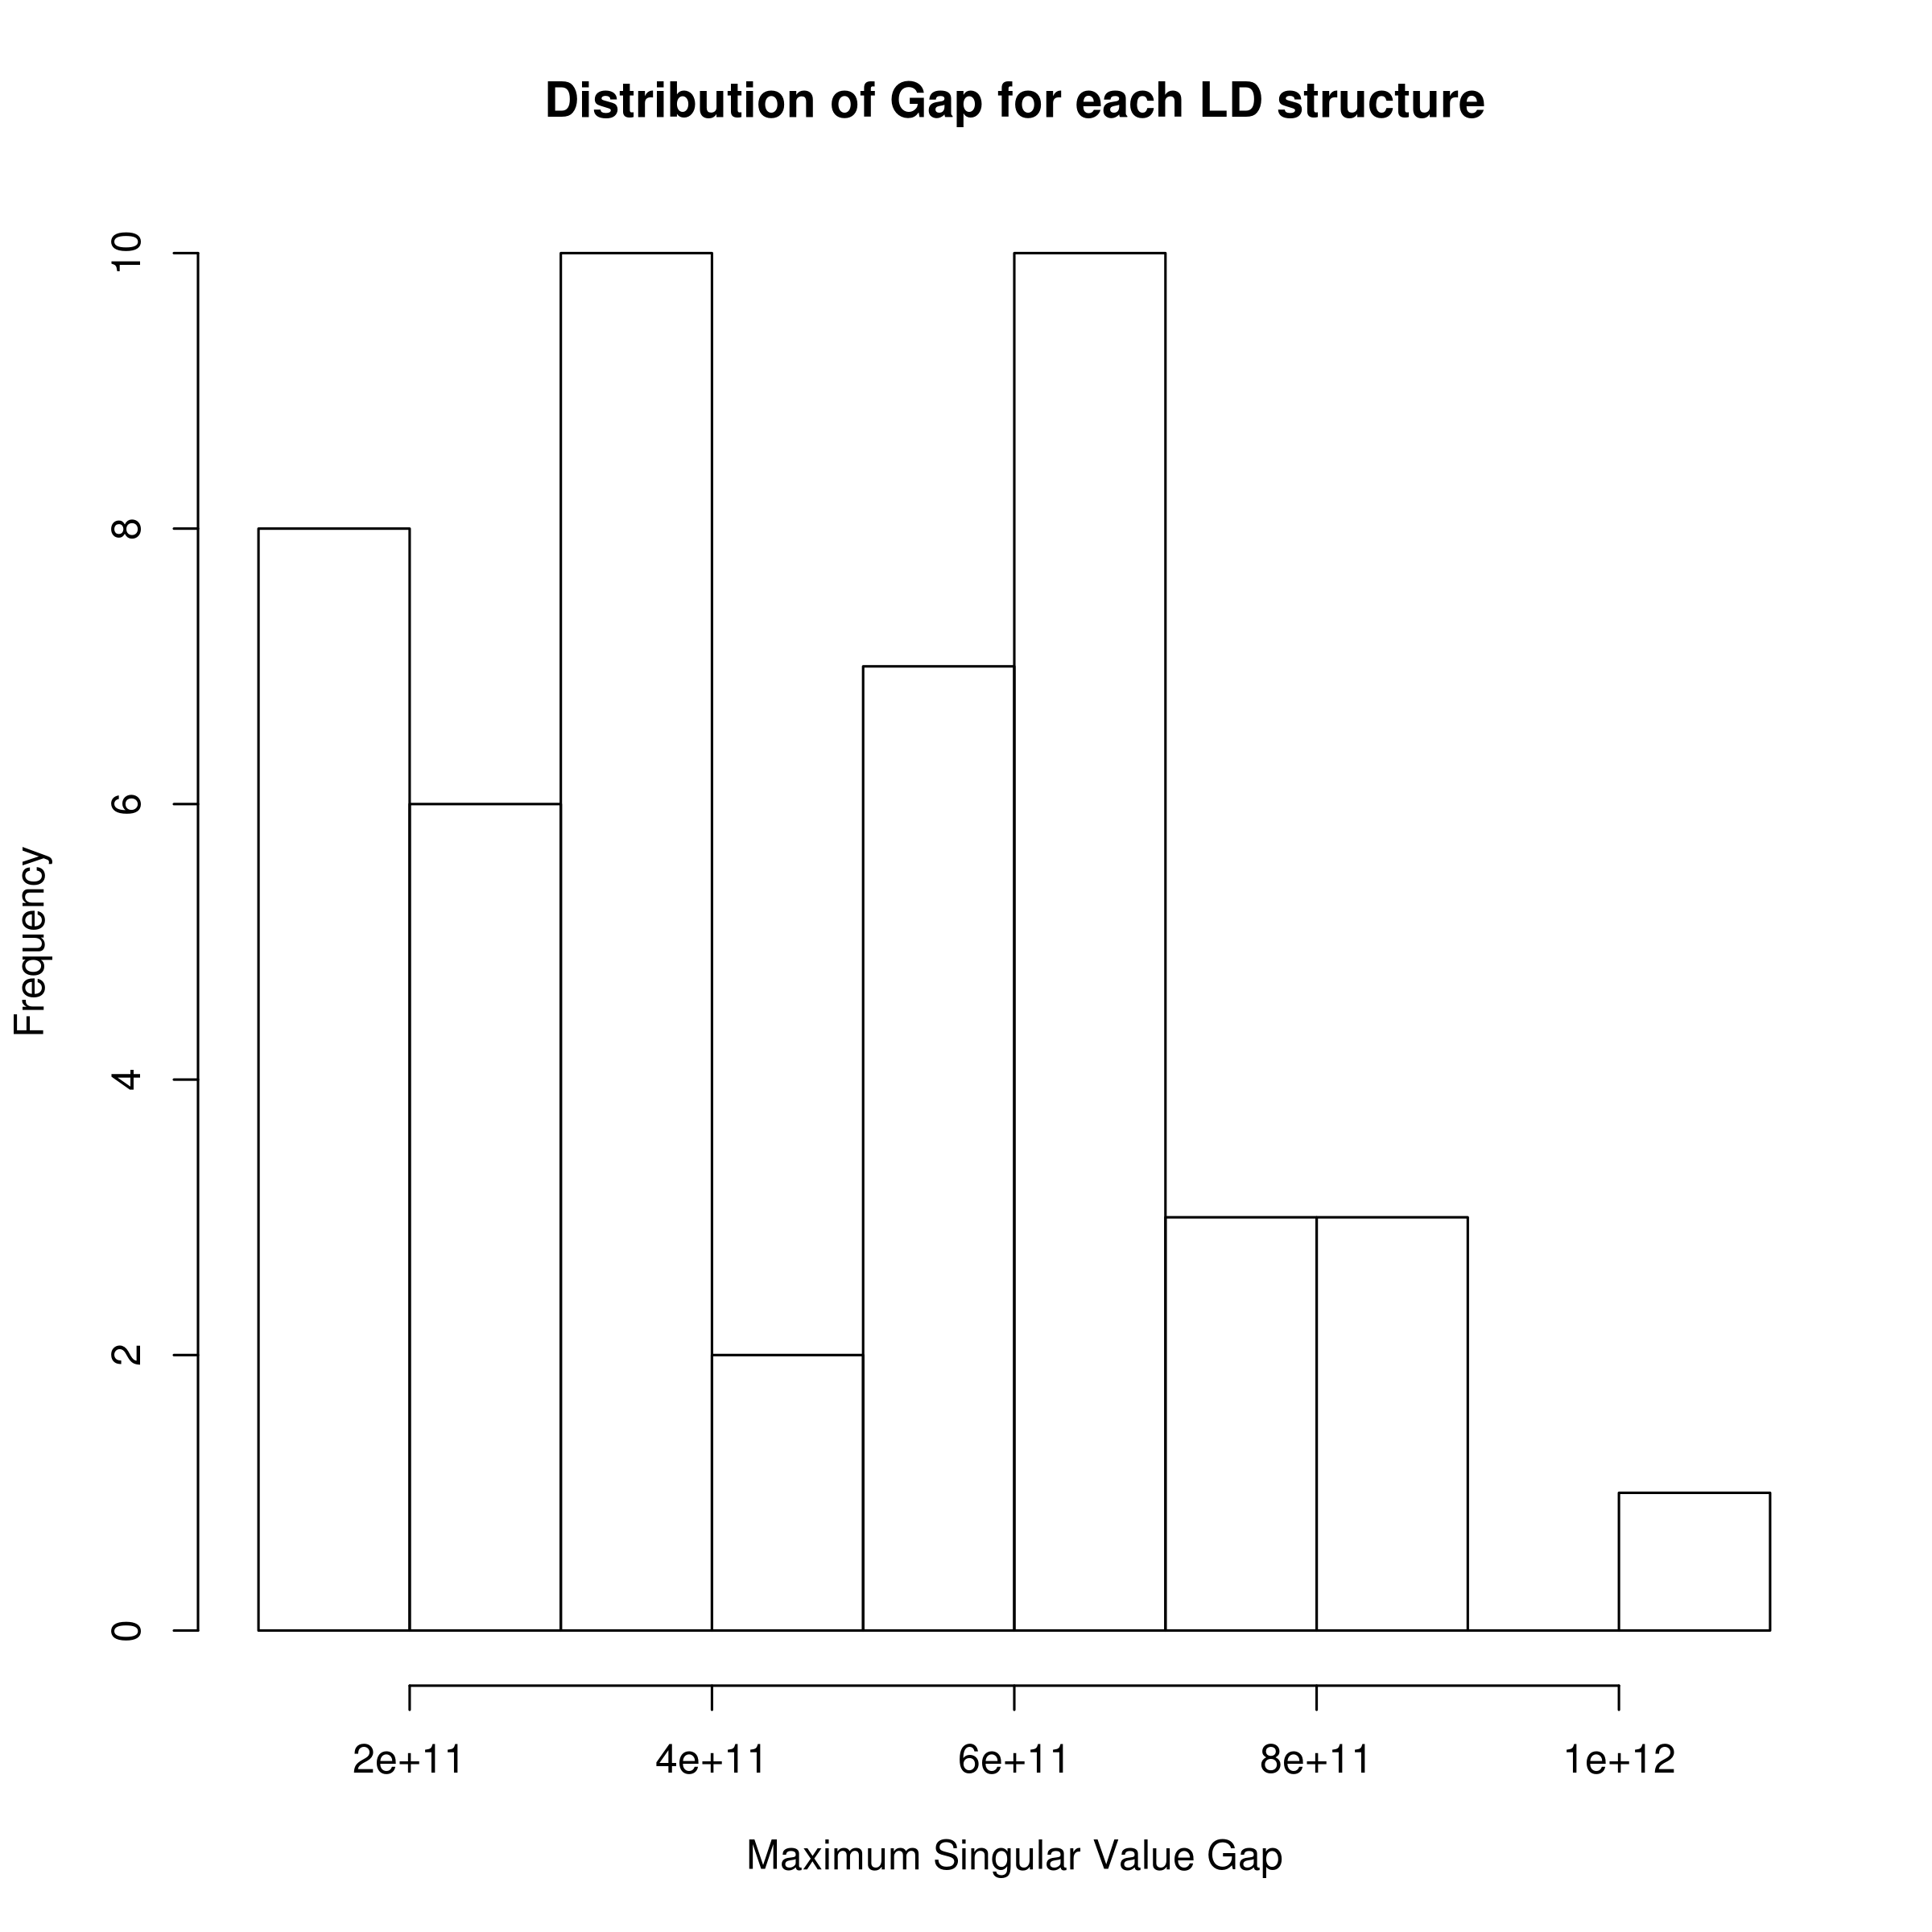
\includegraphics[width=0.5\textwidth]{figure/singular_value_distribution.png}
				\label{fig:singularValueDist}
				\vspace{-20pt}
			\end{figure}
			%\end{wrapfigure}
			
			By employing the \gls{tSVD} as a method for regularization, we were able to solve the ill-posed \cref{eq:shrekEq}, and obtain the estimated heritability.
						
		\subsection{Comparing with \glsentrylong{ldsc}}
			% main difference 
			Conceptually, the fundamental hypothesis of \gls{ldsc} and our algorithm were quite different.
			\gls{ldsc} were based on the ``global'' inflation of test statistic and its relationship to the \gls{LD} pattern.
			\gls{ldsc} hypothesize that the larger the \gls{LD} score, the more likely will the \gls{SNP} be able to ``tag'' the causal \gls{SNP} and the heritability can then be estimated through the regression between the \gls{LD} score and the test statistic.
			
			On the other hand, our algorithm focuses more on the per-\gls{SNP} level.
			Our main idea was that the individual test statistic of each \glspl{SNP} is a combination of its own effect and effect from \glspl{SNP} in \gls{LD} with it. 
			Thus, based on this concept, our algorithm aimed to ``remove'' the inflation of test statistic introduced through the \gls{LD} between \glspl{SNP} and the heritability can be calculated by adding the test statistic of all \glspl{SNP} after ``removing'' the inflation. 
			
			Mathematically, the calculation of \gls{ldsc} and our algorithm were also very different. 
			\gls{ldsc} take the sum of all $R^2$ within a 1cM region as the LD score and regress it against the test statistic to obtain the slope and intercept which represent the heritability and amount of confounding factors respectively. 
			In their model, \gls{ldsc} assume that each \glspl{SNP} will explain the same portion of heritability
			\begin{align}
			 \mathrm{Var}(\beta)&=\frac{h^2}{M}\boldsymbol{I}\\
			 M &= \text{number of SNPs}\notag\\
			 \beta &= \text{vector containing per normalized genotype effect sizes}\notag\\
			 I &= \text{identity matrix}\notag\\
			 h^2 &= \text{heritability}\notag
			\end{align}
			
			As for our algorithm, the whole \gls{LD} matrix were used and inverted to decompose the \gls{LD} from the test statistic. 
			There were no assumption of the amount of heritability explained by each \glspl{SNP}. 
			However, our algorithm does assumed that the null should be 1 and therefore cannot detect the amount of confounding factors. 
			
	\section{Comparing Different LD correction Algorithms}
		\label{sec:ldSim}
		% Might want to remove this section as we no longer use this correction
		Another important consideration in our algorithm is the bias in \gls{LD}.
		In reality, one does not have the population \gls{LD} matrix, instead we have to estimate he \gls{LD} based on various reference panels such as those from the 1000 genome project\citep{Project2012} or the HapMap project\citep{Altshuler2010}.
		These reference panels were a subsamples from the whole population and therefore \gls{LD} estimated from the reference panels usually contains sampling bias.
		Under normal circumstances, because the symmetric nature of sampling error, one would expect there to be little to no bias in the estimated \gls{LD}.
		However, in our algorithm , the $R^2$ is required for the estimation of heritability (\cref{eq:fullShrek}).
		Because we were using the squared \gls{LD}, the sampling error will also be squared, generating a positive bias. 
		
		On average, there were around 500 samples for each super population from the 1000 genome project reference panel.
		Given the relatively small sample size, the sampling bias might be high, therefore lead to systematic bias in the heritability estimation in our algorithm.
		
		To correct for the bias, we would like to apply a \gls{LD} correction algorithm to correct for the bias in the sample \gls{LD}.
		Different authors \citep{Weir1980,Wang2007} have proposed methods for the correction of sample $R^2$ and can be applied for the correction of sample bias in \gls{LD}.
		Therefore we considered the following $R^2$ correction algorithms:
		\begin{align}
		\text{Ezekiel}: \tilde{R^2}&= 1-\frac{n-1}{n-2}(1-\hat{R^2})\label{eq:ezekiel} \\
		\text{Olkin-Pratt}: \tilde{R^2}&=1-\frac{(n-3)(1-\hat{R^2})}{n-2}(1+\frac{2(1-\hat{R^2})}{n})\label{eq:okin} \\
		\text{Pratt}: \tilde{R^2}&=1-\frac{(n-3)(1-\hat{R^2})}{n-2}(1+\frac{2(1-\hat{R^2})}{n-3.3})\label{eq:pratt} \\
		\text{Smith}: \tilde{R^2}&=1-\frac{n}{n-1}(1-\hat{R^2}) \label{eq:smith}\\
		\text{Weir}: \tilde{R^2}&=\hat{R^2}-\frac{1}{2n} \label{eq:weir}
		\end{align}
		where $n$ is the number of samples used to calculate the $R^2$, $\hat{R^2}$ is the sample $R^2$ and $\tilde{R^2}$ is the corrected $R2$.
		
		In order to assess the performance of each individual correction methods, we perform simulations to compare the performance of our algorithm using different \gls{LD} bias correction algorithms.
		Most importantly, we would like to assess the performance of different algorithms not only under one specific \gls{LD} range, but also under the complex \gls{LD} structure observed in real life scenarios.
		First, 5,000 \glspl{SNP} with \gls{maf} $\ge0.1$ were randomly selected from chromosome 22 from the 1000 genome \gls{CEU} haplotypes and were used as an input to HAPGEN2 \citep{Su2011} to simulate 1,000 individuals.
		HAPGEN2 is a simulation tools which simulates new haplotypes as an imperfect mosaic of haplotpyes from a reference panel and the haplotypes that have already been simulated using the \textit{Li and Stephens} (LS) model of \gls{LD} \citep{Li2003}.
		This allow us to simulate genotypes with \gls{LD} structures comparable to those observed in \gls{CEU} population. 
		Of those 5,000 \glspl{SNP}, 100 of them were randomly selected as the causal variant. 
		\citet{Orr1998} suggested that the exponential distribution can be used to approximate the genetic architecture of adaptation. 
		As a result of that, we used the exponential distribution with $\lambda=1$ as an approximation to the effect size distribution:
		\begin{align}
		\theta&=\mathrm{exp}(\lambda=1)\notag\\
		\beta&=\pm\sqrt{\frac{\theta \times h^2}{\sum \theta}}
		\label{eq:randomEffect}
		\end{align}
		with a random direction of effect.
		The simulated effects were then randomly distributed to each causal \glspl{SNP}.
			
		Using the normalized genotype of the causal \glspl{SNP} of each individual ($\boldsymbol{X}$), the vector of effect size ($\boldsymbol{\beta}$) we can simulate a phenotype with target heritability of $h^2$ as
		\begin{align}
		\epsilon_i&\sim N(0,\sqrt{\mathrm{Var}(\boldsymbol{X\beta})\frac{1-h^2}{h^2}} )\notag\\
		\boldsymbol{\epsilon} &= (\epsilon_1,\epsilon_2,...,\epsilon_n)^t\notag\\
		\boldsymbol{y} &= \boldsymbol{X\beta}+\boldsymbol{\epsilon}
		\label{eq:simulationOfPhenotype}
		\end{align}
		To simulate the whole spectrum of heritability, we varies the target $h^2$ from 0 to 0.9 with increment of 0.1.
		
		The test statistics of association between the genotype and phenotype were then calculated using PLINK \citep{Purcell2007}.
		Resulting test statistic were then input to our algorithm to estimate the heritability, using different \gls{LD} correction algorithms.
		An independent 500 samples, a size roughly correpsond to the average sample size of each super population form the 1,000 genome project,  were simulated as a reference panel for the calculation of \gls{LD} matrix.
		This is because in reality, one usually doesn't have assess to the sample genotype and has to rely on an independent reference panel for the calculation of \gls{LD} matrix. 
		Thus this simulation procedure should provide a realistic representation of how the algorithm was commonly used in real life scenario.
		
		The whole process will be repeated 50 times such that a distribution of the estimate can be obtained. 
		In summary, we simulate a large population of samples (e.g. $50\times1,000+500 = 50,500$) where 500 samples were randomly selected as a reference panel. 
		In the subsequent iteration of simulation, 1,000 samples were randomly selected from the population \textit{without replacement} and estimation were performed.
		\begin{enumerate}
			\item Randomly select 5,000 \glspl{SNP} with \gls{maf}$>0.1$ from chromosome 22
			\item Simulate 500 samples using HAPGEN2 and used as a reference panel
			\item Randomly generate 100 effect size with following \cref{eq:randomEffect}
			\item Randomly assign the effect size to 100 \glspl{SNP} with heritability from 0 to 0.9 (increment of 0.1)
			\item Simulate 1,000 samples using HAPGEN2 and calculate their phenotype according to \cref{eq:simulationOfPhenotype} 
			\item Perform heritability estimation using our algorithm with different ways of \gls{LD} correction
			\item Repeat step 5-6 50 times
		\end{enumerate}
		
		\section{Comparison with Other Algorithms}
		After identifying the optimal \gls{LD} correction algorithm, we would like to compare our algorithm to existing methods for the performance in estimating the narrow sense heritability.
		It is important for us to consider most if not all conditions in our simulation. 
		Therefore, we would like to simulate quantitative traits and case control studies with different number of causal \glspl{SNP}; quantitative traits with extreme effect sizes; and last but not least, quantitative traits with extreme phenotype selection.
		
		Currently, the only other algorithm that is capable to estimate the narrow sense heritability using only test statistic is the \gls{ldsc} \citep{Bulik-Sullivan2015}. 
		On the other hand, \gls{gcta} \citep{Yang2011} is commonly used for heritability estimation in \gls{GWAS} data. 
		Therefore, we choose to compare the performance of our algorithm to that of \gls{ldsc} and \gls{gcta}.
		It is important to note that as we are assessing the performance of the algorithms through controlled simulation, there should be little confounding factors. 
		For \gls{ldsc}, the default intercept estimation function allows it to estimate and correct for confounding factors with an increase in \gls{se}. 
		The simulation will therefore be unfair to \gls{ldsc} with intercept estimation, as the \gls{se} is increased yet there are little confounding factors for it to correct.
		Thus, we also simulate \gls{ldsc} with a fixed intercept (-{}-no-intercept) parameters to avoid bias against \gls{ldsc}.	
		
		\subsection{Sample Size}
			One important consideration in our simulation was the number of sample simulated. 
			The sample size was the most important parameter in determining the standard error of the heritability estimation. 
			As sample size increases, study will be more representative of the true population. 
			The increased number of information also means a better estimation of parameters, therefore a smaller \acrfull{se}.
			% awk -F "\t" '{print $2"\t"$9}' full | uniq | sed -e 's/[^0-9[:space:]]//g' | awk '{for(i=2;i<=NF;++i)j+=$i; print $1" "j; j=0}' | sort | uniq  %script for text mining
			Based on information from \gls{GWAS} catalog\citep{Welter2014}, we calculate the sample size distribution using simple text mining and exclude studies with conflicting sample size information in multiple entries. 
			The average sample size for all \gls{GWAS} recorded on the \gls{GWAS} catalog was 7,874, with a median count of 2,506 and a lower quartile at 940 (\cref{fig:gwasCata}). 
			We argue that if the algorithm works for studies with a small sample size (e.g lower quartile sample size), then it should perform even better when the sample size is larger. 
			Thus, we only simulate 1,000 samples in our simulation, which roughly represent the lower quartile sample size range.
				
			\begin{wrapfigure}{R}{8cm}
				\centering
				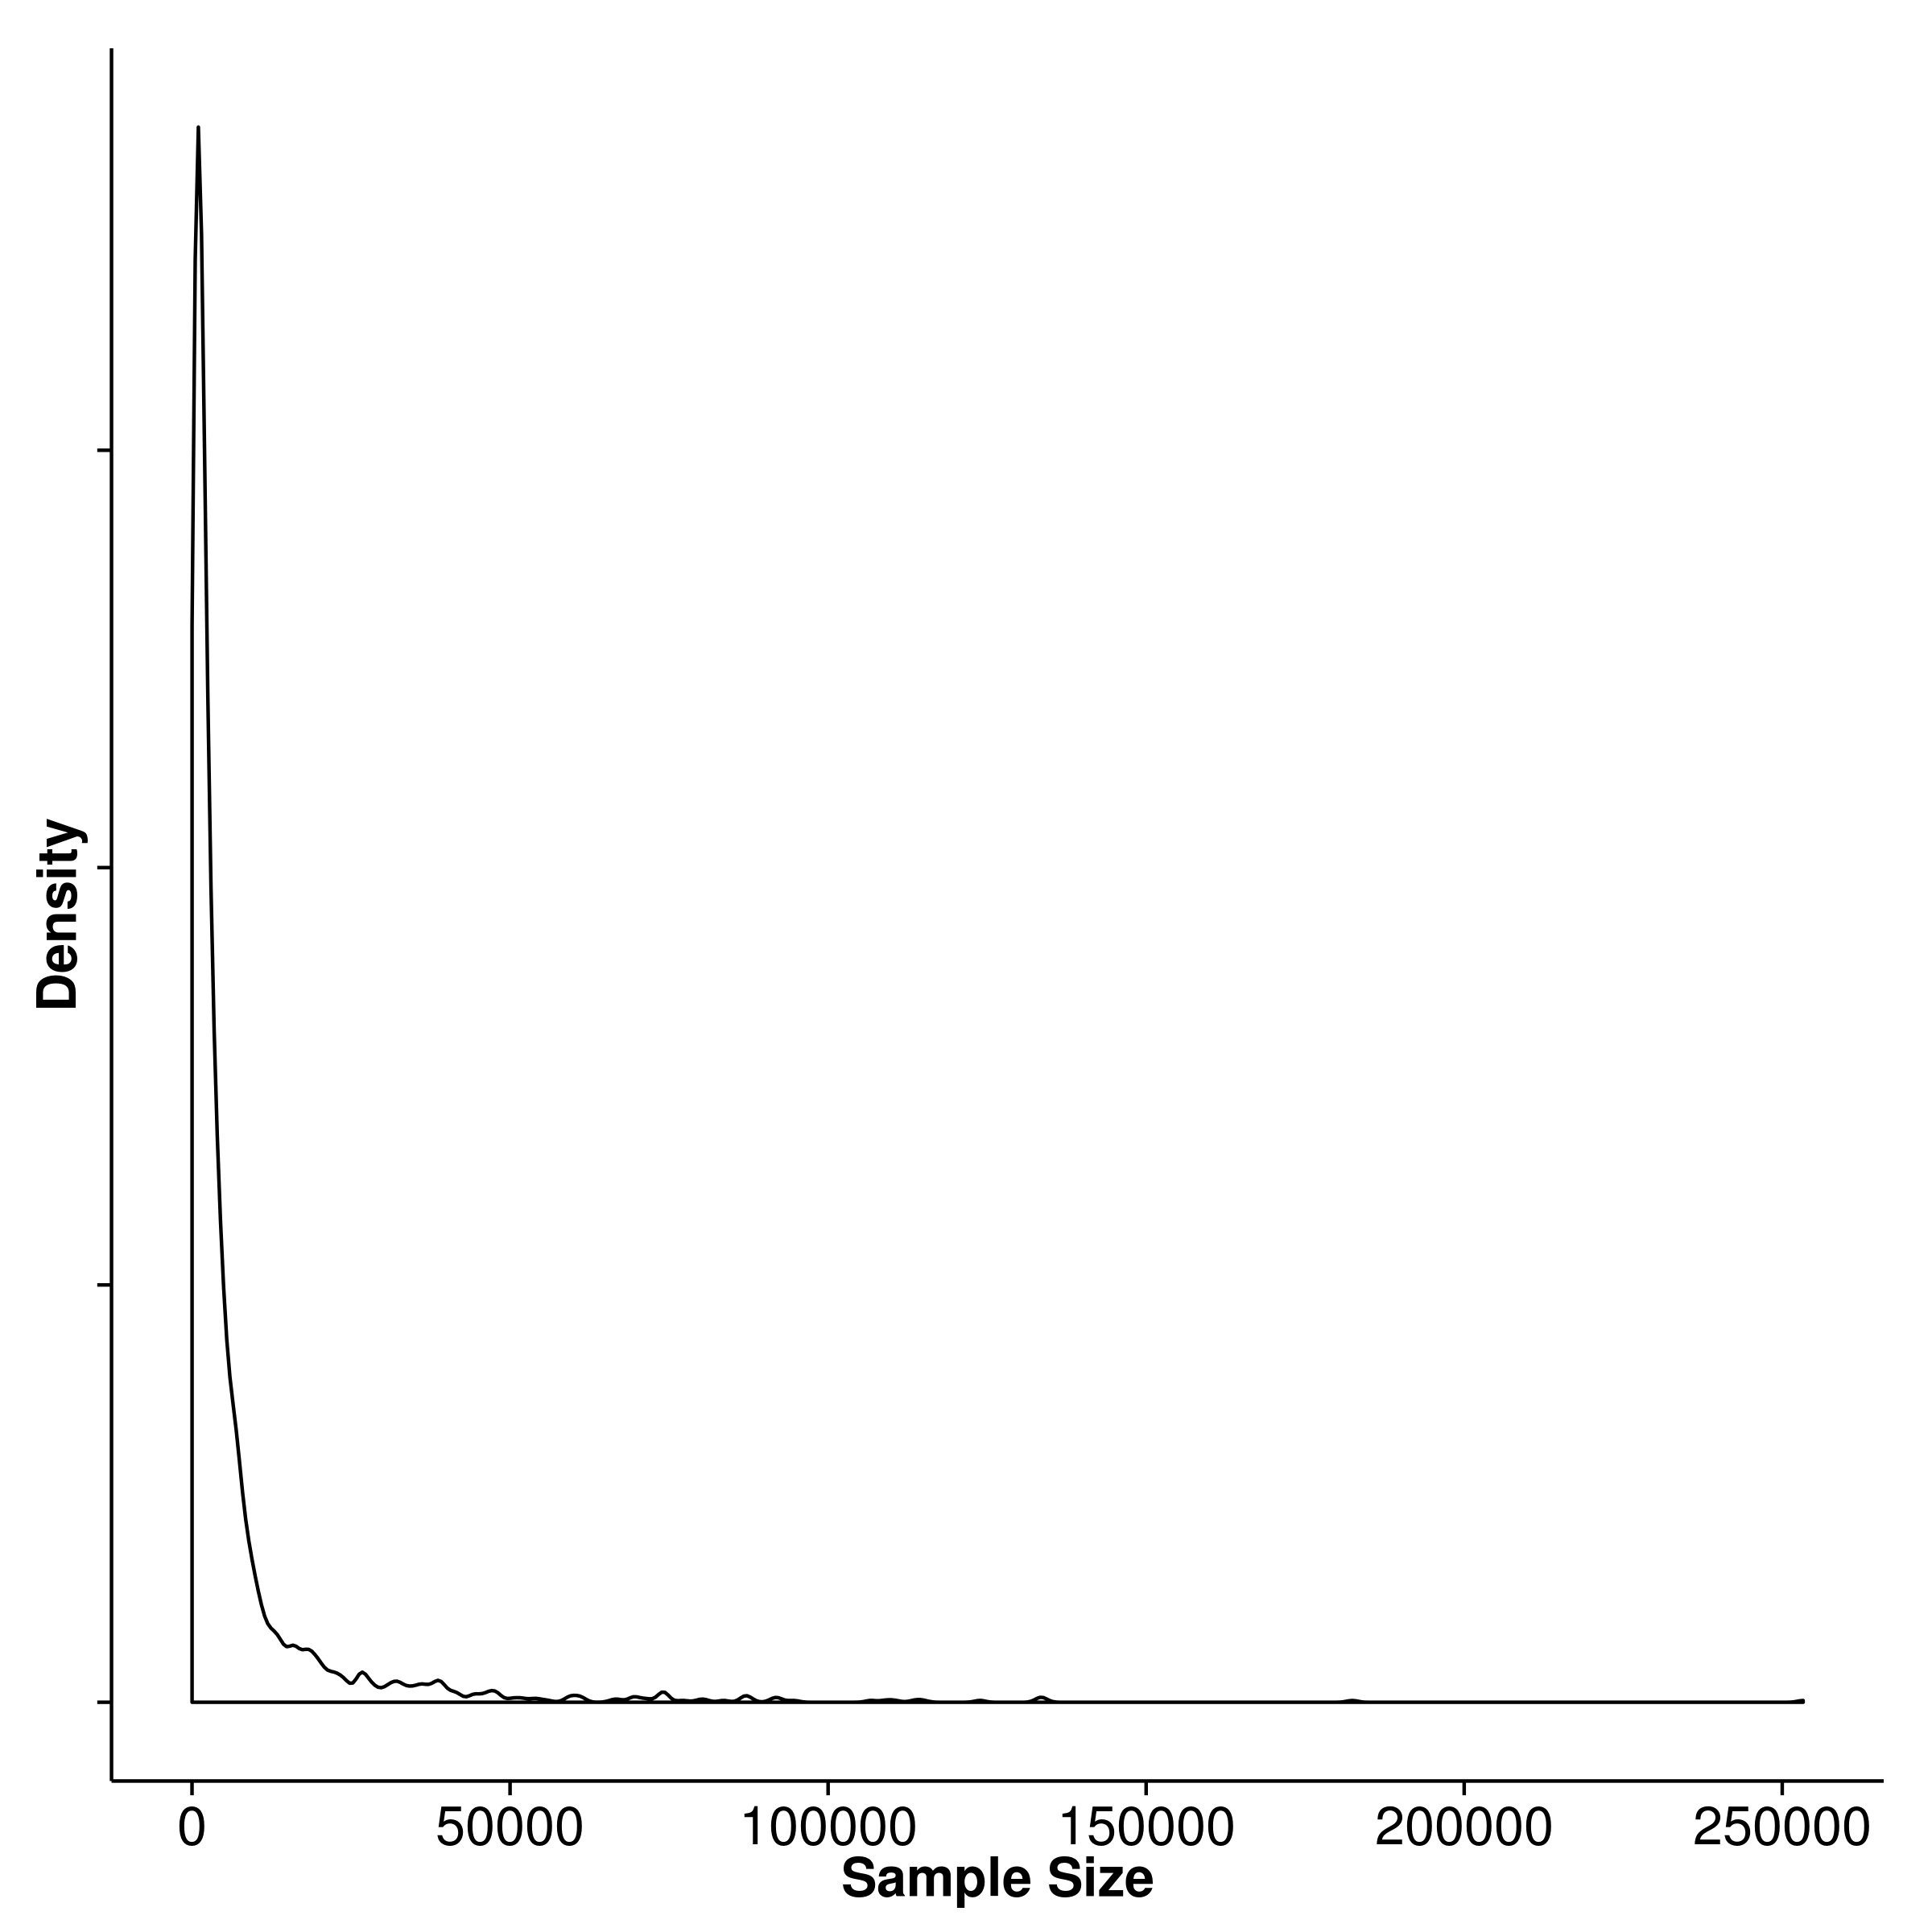
\includegraphics[width=0.5\textwidth]{figure/gwasSampleSize.png}
				\caption[GWAS Sample Size distribution]{
					\gls{GWAS} sample size distribution.
				}
				\label{fig:gwasCata}
			\end{wrapfigure}
		\subsection{Number of SNPs in Simulation}
			Another consideration in the simulation was the number of \glspl{SNP} included.
			In a typical \gls{GWAS} study, there are usually a larger number of \glspl{SNP} when compared to the sample size. 
			For example, in the \gls{pgc} \glng{scz} \gls{GWAS}, more than 9 million \glspl{SNP} were included, with around 700,000 \glspl{SNP} on chromosome 1.
			In reality, the estimation of heritability based on 700,000 \glspl{SNP} can be done quickly.
			However, in our simulation, we will repeat the calculation $50(\text{iteration})\times10(\text{number of heritability})=500$ times for \emph{each} condition tested. 
			The time required to finish all the simulation quickly becomes infeasible given the large amount of \glspl{SNP}.
			To compromise, we simulate a total of 50,000 \glspl{SNP} from chromosome 1 as a balance between run time of simulation and the total \glspl{SNP} simulated.
			With 50,000 \glspl{SNP}, there are roughly 200 \glspl{SNP} within a 1 \gls{mb} region.
		\subsection{Genetic Architecture}
			Of all simulation parameter, the genetic architecture was the most complicated and important parameter. 
			The \gls{LD} pattern, the number of causal \glspl{SNP}, the effect size of the causal \glspl{SNP} and the heritability of the trait were all important factors contribute to the genetic architecture of a trait. 
		
			First and foremost, because the aim of the algorithm was to estimating the heritability of the trait, it is important that the algorithm works for traits from different heritability spectrum.
			We therefore simulate traits with heritability ranging from 0 to 0.9, with increment of 0.1.
		
			Secondly, in real life scenario, the ``causal'' variant might not be readily included on the \gls{GWAS} chip and were only ``tagged'' by \glspl{SNP} included on the \gls{GWAS} chip.
			However, to simplify our simulation, all ``causal'' variants were included in our simulation (e.g. perfectly ``tagged'')
		
			Thirdly, to obtain a realistic \gls{LD} pattern, we simulate the genotypes using the HAPGEN2 programme\citep{Su2011}, using the 1000 genome \gls{CEU} haplotypes as an input.
			In a typical \gls{GWAS} , one usually only have power in detecting ``common variants'', defined as variants with \gls{maf} $\ge 0.05$.
			We therefore only consider scenario with ``common'' variants and only use \glspl{SNP} with \gls{maf} $\ge0.05$ in the \gls{CEU} haplotypes as an input to HAPGEN2 to simulate 1,000 samples.
			
			Finally, we would like to simulate traits with different inheritance model such as oligogenic traits and polygenic traits.
			We therefore varies the number of causal \glspl{SNP} ($k$) with $k\in\{5, 10, 50, 100, 250, 500\}$.
			The effect size were then simulated using \cref{eq:randomEffect} and the phenotype were simulated using \cref{eq:simulationOfPhenotype}.
			
			For \gls{gcta}, the sample genotypes were provided to calculate the genetic relationship matrix and the sample phenotype were used in combination with the genetic relationship matrix to estimate the heritability.
			
			On the other hand, for \gls{ldsc} and our algorithm, an independent 500 samples were simulated as the reference panel for the calculation of \gls{LD} scores and \gls{LD}matrix, mimicking real life scenario where an independent reference panel were used. 
			The genotype association test statistics calculated from PLINK and the \gls{LD} score / \gls{LD} matrix were then used for the estimation of heritability for \gls{ldsc} and our algorithm respectively. 
			
			The whole process will be repeated 50 times such that a distribution of the estimate can be obtained.
			10 independent population were simulated and the whole processed were repeated.
			In summary, the simulation follows the following procedures:
			\begin{enumerate}
				\item Randomly select 50,000 \glspl{SNP} with \gls{maf}$>0.1$ from chromosome 1
				\item Simulate 500 samples using HAPGEN2 and used as a reference panel
				\item Randomly generate $k$ effect size with $k \in \{5,10,50,100,250,500\}$ following \cref{eq:randomEffect}, with heritability ranging from 0 to 0.9 (increment of 0.1)
				\item Randomly assign the effect size to $k$ \glspl{SNP}
				\item Simulate 1,000 samples using HAPGEN2 and calculate their phenotype according to \cref{eq:simulationOfPhenotype}
				\item Perform heritability estimation using our algorithm, \gls{gcta}, \gls{ldsc} with fixed intercept and \gls{ldsc} with intercept estimation.
				\item Repeat step 5-6 50 times
				\item Repeat step 1-7 10 times
			\end{enumerate}
		
		\subsection{Extreme Effect Size}
		On top of the original quantitative trait simulation, another condition we were interested in was the performance of the algorithms when there is a small amount of \glspl{SNP} with a much larger effect size.
		This can be observed in disease such as Hirschsprung's disease.
		The Hirschsprung's disease is a congenital disorder where deleterious mutations on \textit{RET} account for $\approx$50\% of the familial cases yet there is still missing heritability, suggesting that there might be more variants with small effects that have not been identified \citep{Gui2013}.
		
		To simulate extreme effect size, we consider scenarios where $m$ \glspl{SNP} accounts 50\% of all the effect size with $m\in\{1,5,10\}$.
		The effect size was then calculated as
		\begin{align}
		\beta_{eL} &= \pm\sqrt{\frac{0.5h^2}{m}} \notag\\
		\beta_{eS} &= \pm\sqrt{\frac{0.5h^2}{100-m}} \notag\\
		\beta &= \{\beta_{eL}, \beta_{eS}\}
		\label{eq:extremEffect}
		\end{align}
		The effect size were then randomly assigned to 100 causal \glspl{SNP} and phenotype will be calculated as in \cref{eq:simulationOfPhenotype}.
		The simulation procedure then becomes
		\begin{enumerate}
			\item Randomly select 50,000 \glspl{SNP} with \gls{maf}$>0.1$ from chromosome 1
			\item Simulate 500 samples using HAPGEN2 and used as a reference panel
			\item Randomly generate 100 effect size where $m$ has extreme effect, following \cref{eq:extremEffect}, with $m\in\{1,5,10\}$
			\item Randomly assign the effect size to 100 \glspl{SNP}
			\item Simulate 1,000 samples using HAPGEN2 and calculate their phenotype according to \cref{eq:simulationOfPhenotype}
			\item Perform heritability estimation using our algorithm, \gls{ldsc} with fixed intercept, \gls{ldsc} with intercept estimation and \gls{gcta}
			\item Repeat step 5-6 50 times
			\item Repeat step 1-7 10 times
		\end{enumerate}
		
		\subsection{Case Control Studies}
		The simulation of case control studies was similar to the simulation of quantitative trait. 
		However, there were two additional parameters to consider: the population prevalence and the observed prevalence.
		These parameters were required to simulate the samples under a liability model for case control studies.

		Although there were only two additional parameter, it is significantly more challenging for to simulate when compared to the simulation of quantitative traits.
		It is mainly because of the number of samples required to simulate adequate samples under the liability threshold model.
		Take for example, if one like to simulate a trait with population prevalence of $p$ and observed prevalence of $q$ and would like to have $n$ cases in total, one will have to simulate $\min(\frac{n}{p}, \frac{n}{q})$ samples.
		Considering the scenario where the observed prevalence is 50\%, the population prevalence is 1\%, if we want to simulate 1,000 cases, a minimum of 100,000 samples will be required.
		
		Given limited computer resources, it will be infeasible for us to simulate 1,000 cases with 50,000 \glspl{SNP} when the population prevalence is small.
		To simplify the simulation and reduce the burden of computation, we limited the observed prevalence to 50\% and varies the population prevalence $p$ such that $p\in\{0.5, 0.1, 0.05, 0.01\}$.
		Most importantly, we reduce the number of \glspl{SNP} simulated to 5,000 on chromosome 22 instead of 50,000 \glspl{SNP} on chromosome 1. 
		The change from chromosome 1 to chromosome 22 allow us to reduce the number of \glspl{SNP} without changing much of the \gls{SNP} density. 
		We acknowledged that the current simulation was relatively brief, however, it should serves as a prove of concept simulation to study the performance of the algorithms under the case control scenario.
		
		In the case control simulation, we randomly select 5,000 \glspl{SNP} from chromosome 22 with \gls{maf} $\ge0.1$ in the \gls{CEU} haplotypes as an input to HAPGEN2. 
		We then randomly select 100 \glspl{SNP} with effect size simulated based on \cref{eq:randomEffect}.
		In order to simulate a case control samples with 1,000 cases, we then simulate $\frac{1,000}{p}$ samples and calculate their phenotype using \cref{eq:simulationOfPhenotype}.
		The phenotype was then standardized and cases were defined as sample with phenotype passing the liability threshold with respect to $p$.
		An equal amount of samples were then randomly selected from samples with phenotype lower than the liability threshold and defined as controls.
			
		Finally, the case control simulation were performed as:
		\begin{enumerate}
			\item Randomly select 5,000 \glspl{SNP} with \gls{maf}$>0.1$ from chromosome 22
			\item Simulate 500 samples using HAPGEN2 and used as a reference panel
			\item Randomly generate 100 effect size following  \cref{eq:randomEffect}
			\item Randomly assign the effect size to 100 \glspl{SNP}
			\item Simulate $\frac{1,000}{p}$ samples using HAPGEN2 and calculate their phenotype according to \cref{eq:simulationOfPhenotype}
			\item Define case control status using the liability threshold and randomly select same number of case and controls for subsequent simulation
			\item Perform heritability estimation using our algorithm, \gls{ldsc} with fixed intercept, \gls{ldsc} with intercept estimation and \gls{gcta}
			\item Repeat step 5-7 50 times
			\item Repeat step 1-8 10 times
		\end{enumerate}
		
		\subsection{Extreme Phenotype Selection}
		The simulation of extreme phenotype selection was the same as the quantitative trait simulation. 
		The only difference being that instead of using all samples for heritability estimation, we only use the extreme 10\% of samples among the population for the heritability estimation.
		In brief, instead of simulating 1,000 samples, we simulate 5,000 samples following the exact procedure in the quantitative trait simulation with random effect size.
		However, after simulation of the phenotype using \cref{eq:simulationOfPhenotype}, we standardize the phenotype and only select the top 10\% and bottom 10\% samples (500 samples each) from the sample distribution.
		We then perform the same simulation procedure as in the quantitative trait simulation with random effect size.
		
		It was noted that the extreme phenotype selection were not supported by the \gls{ldsc} and \gls{gcta}.
		To allow comparison in such scenario, we apply the extreme phenotype adjustment from \citet{Sham2014} to the estimation obtained from \gls{ldsc} and \gls{gcta}.
	
	\section{Simulation with Real Data}
	\section{Application to Real Data}
	
	
	\section{Result}
		The heritabilibty estimation were implemented in \gls{shrek} and is available on \url{https://github.com/choishingwan/shrek}.  
		\subsection{LD Correction}
		\begin{figure}[t]
			\centering
			\subfloat[Mean Estimation]{
				\scalebox{.4}{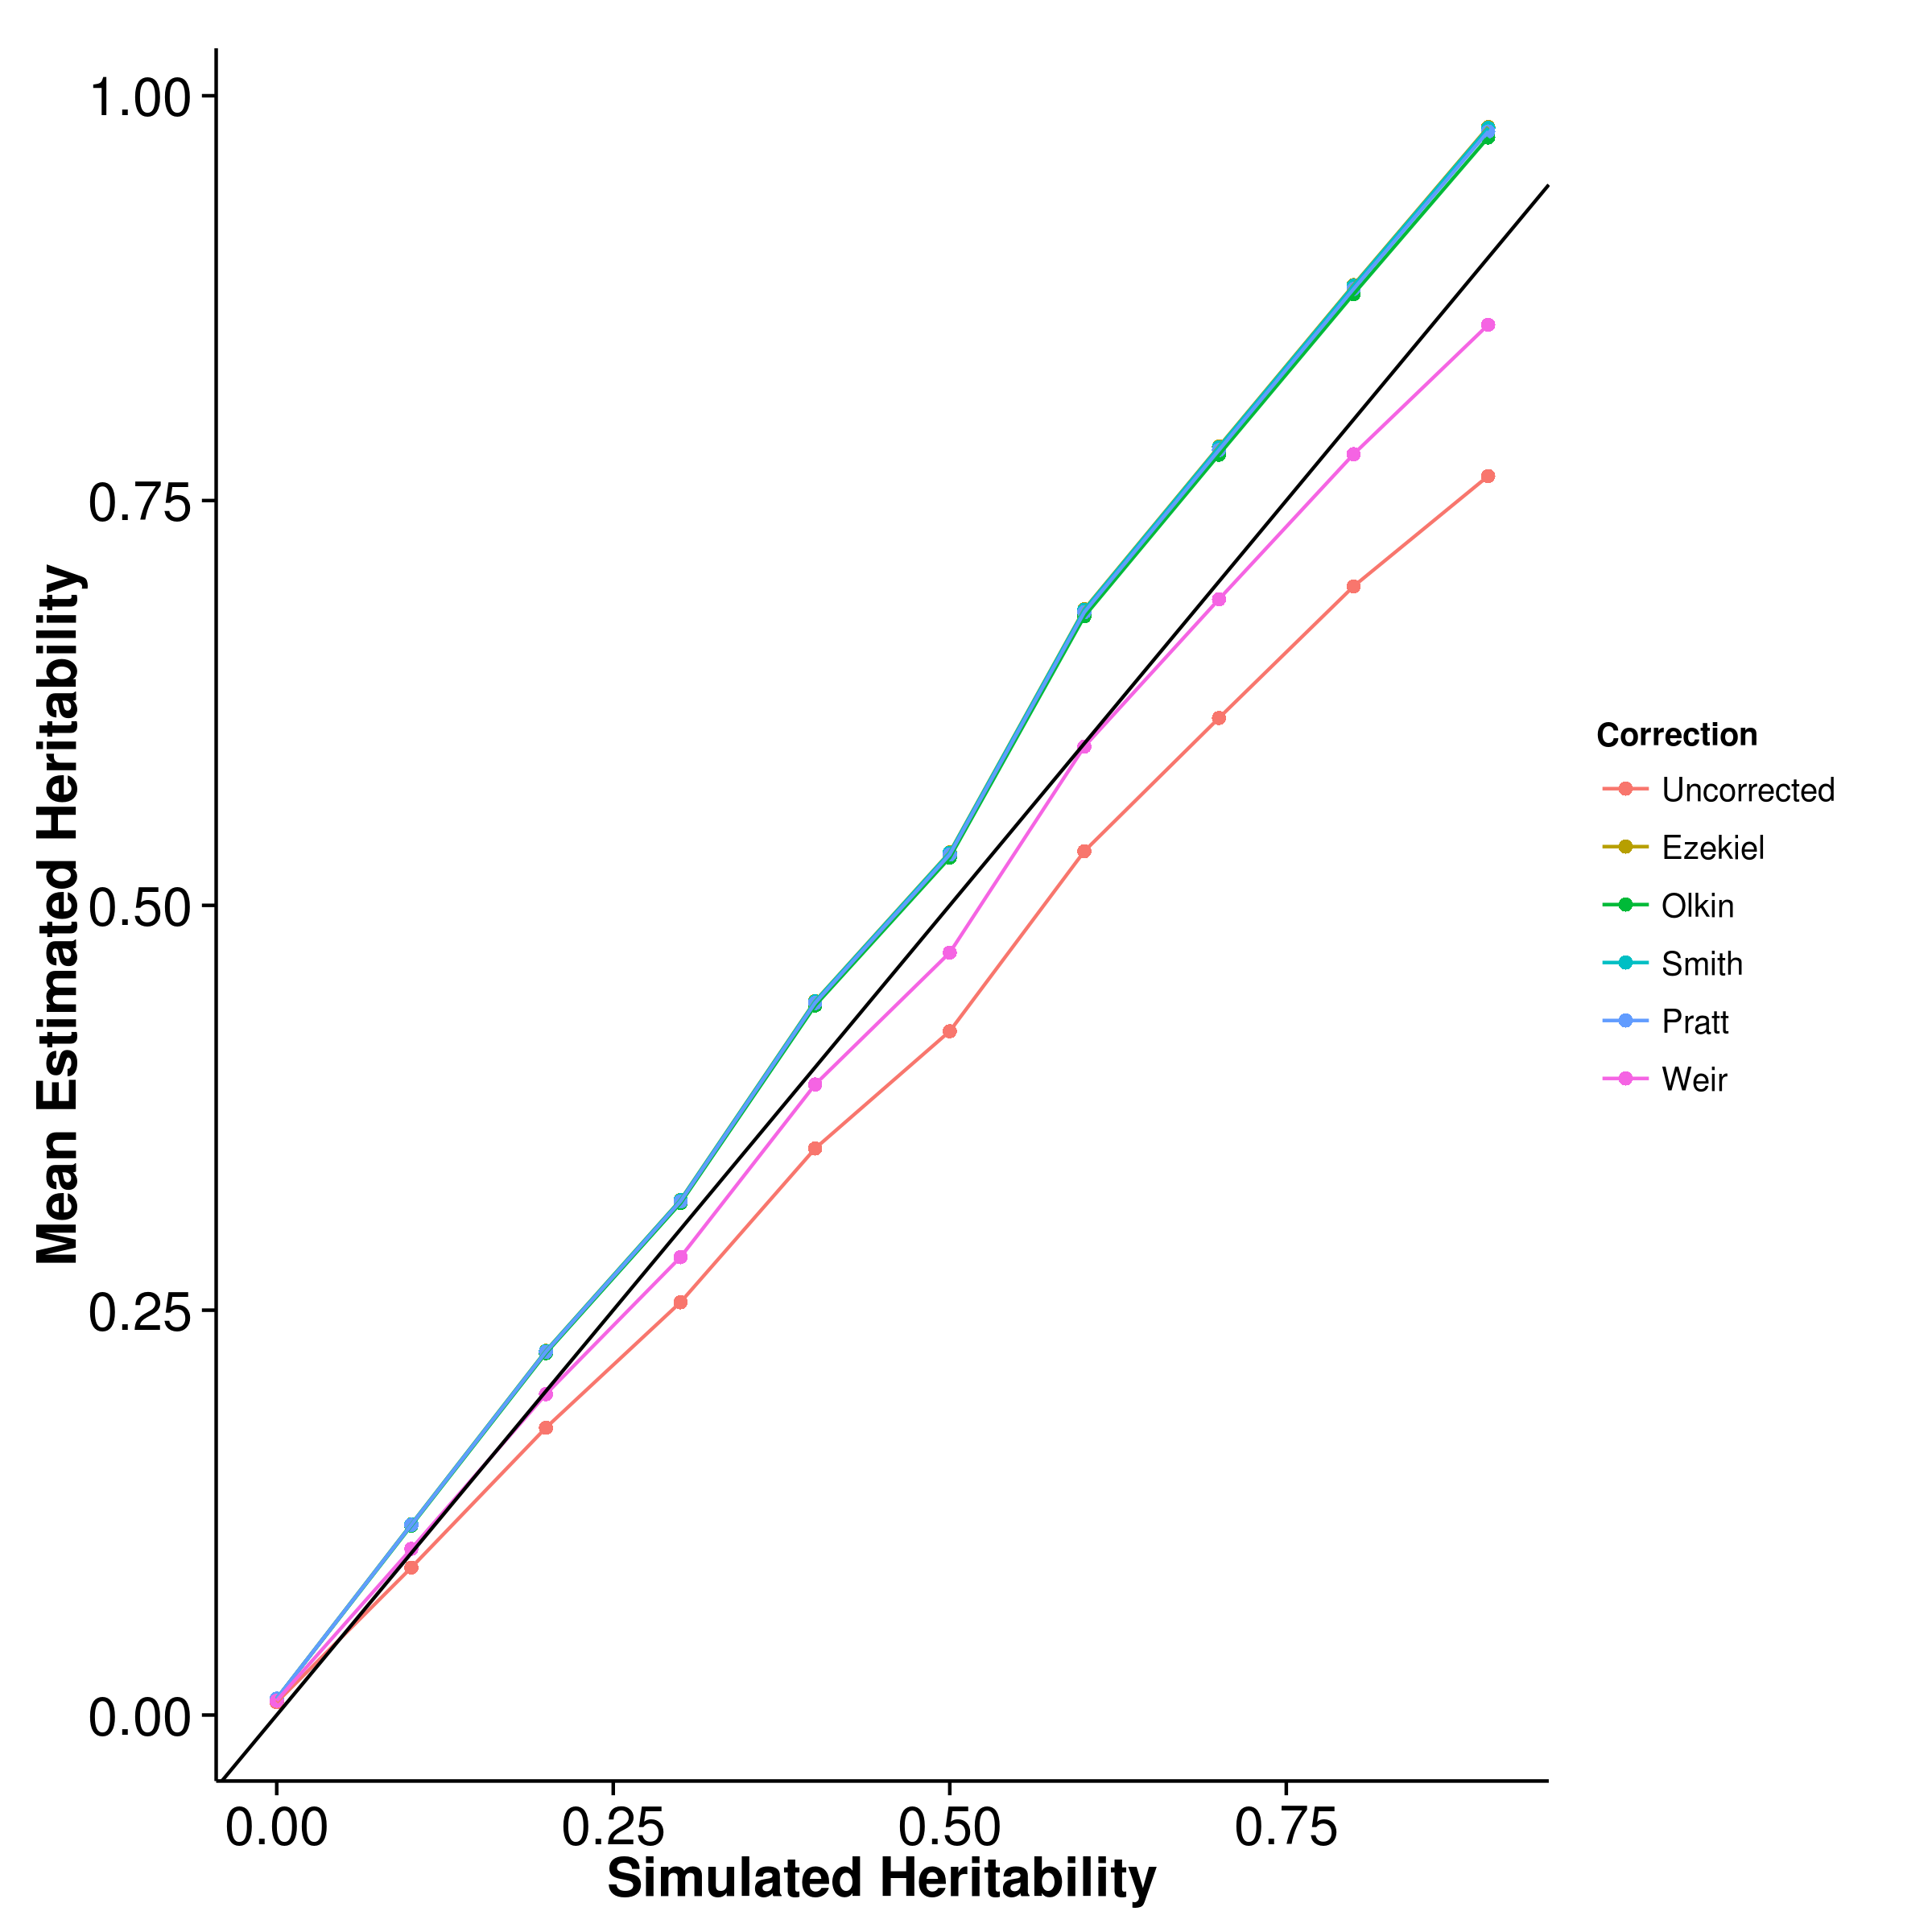
\includegraphics{figure/quantitative/ld_correct/ldCom_mean.png}}
				\label{fig:meanLDCor}
			}
			\subfloat[Empirical Variance]{
				\scalebox{.4}{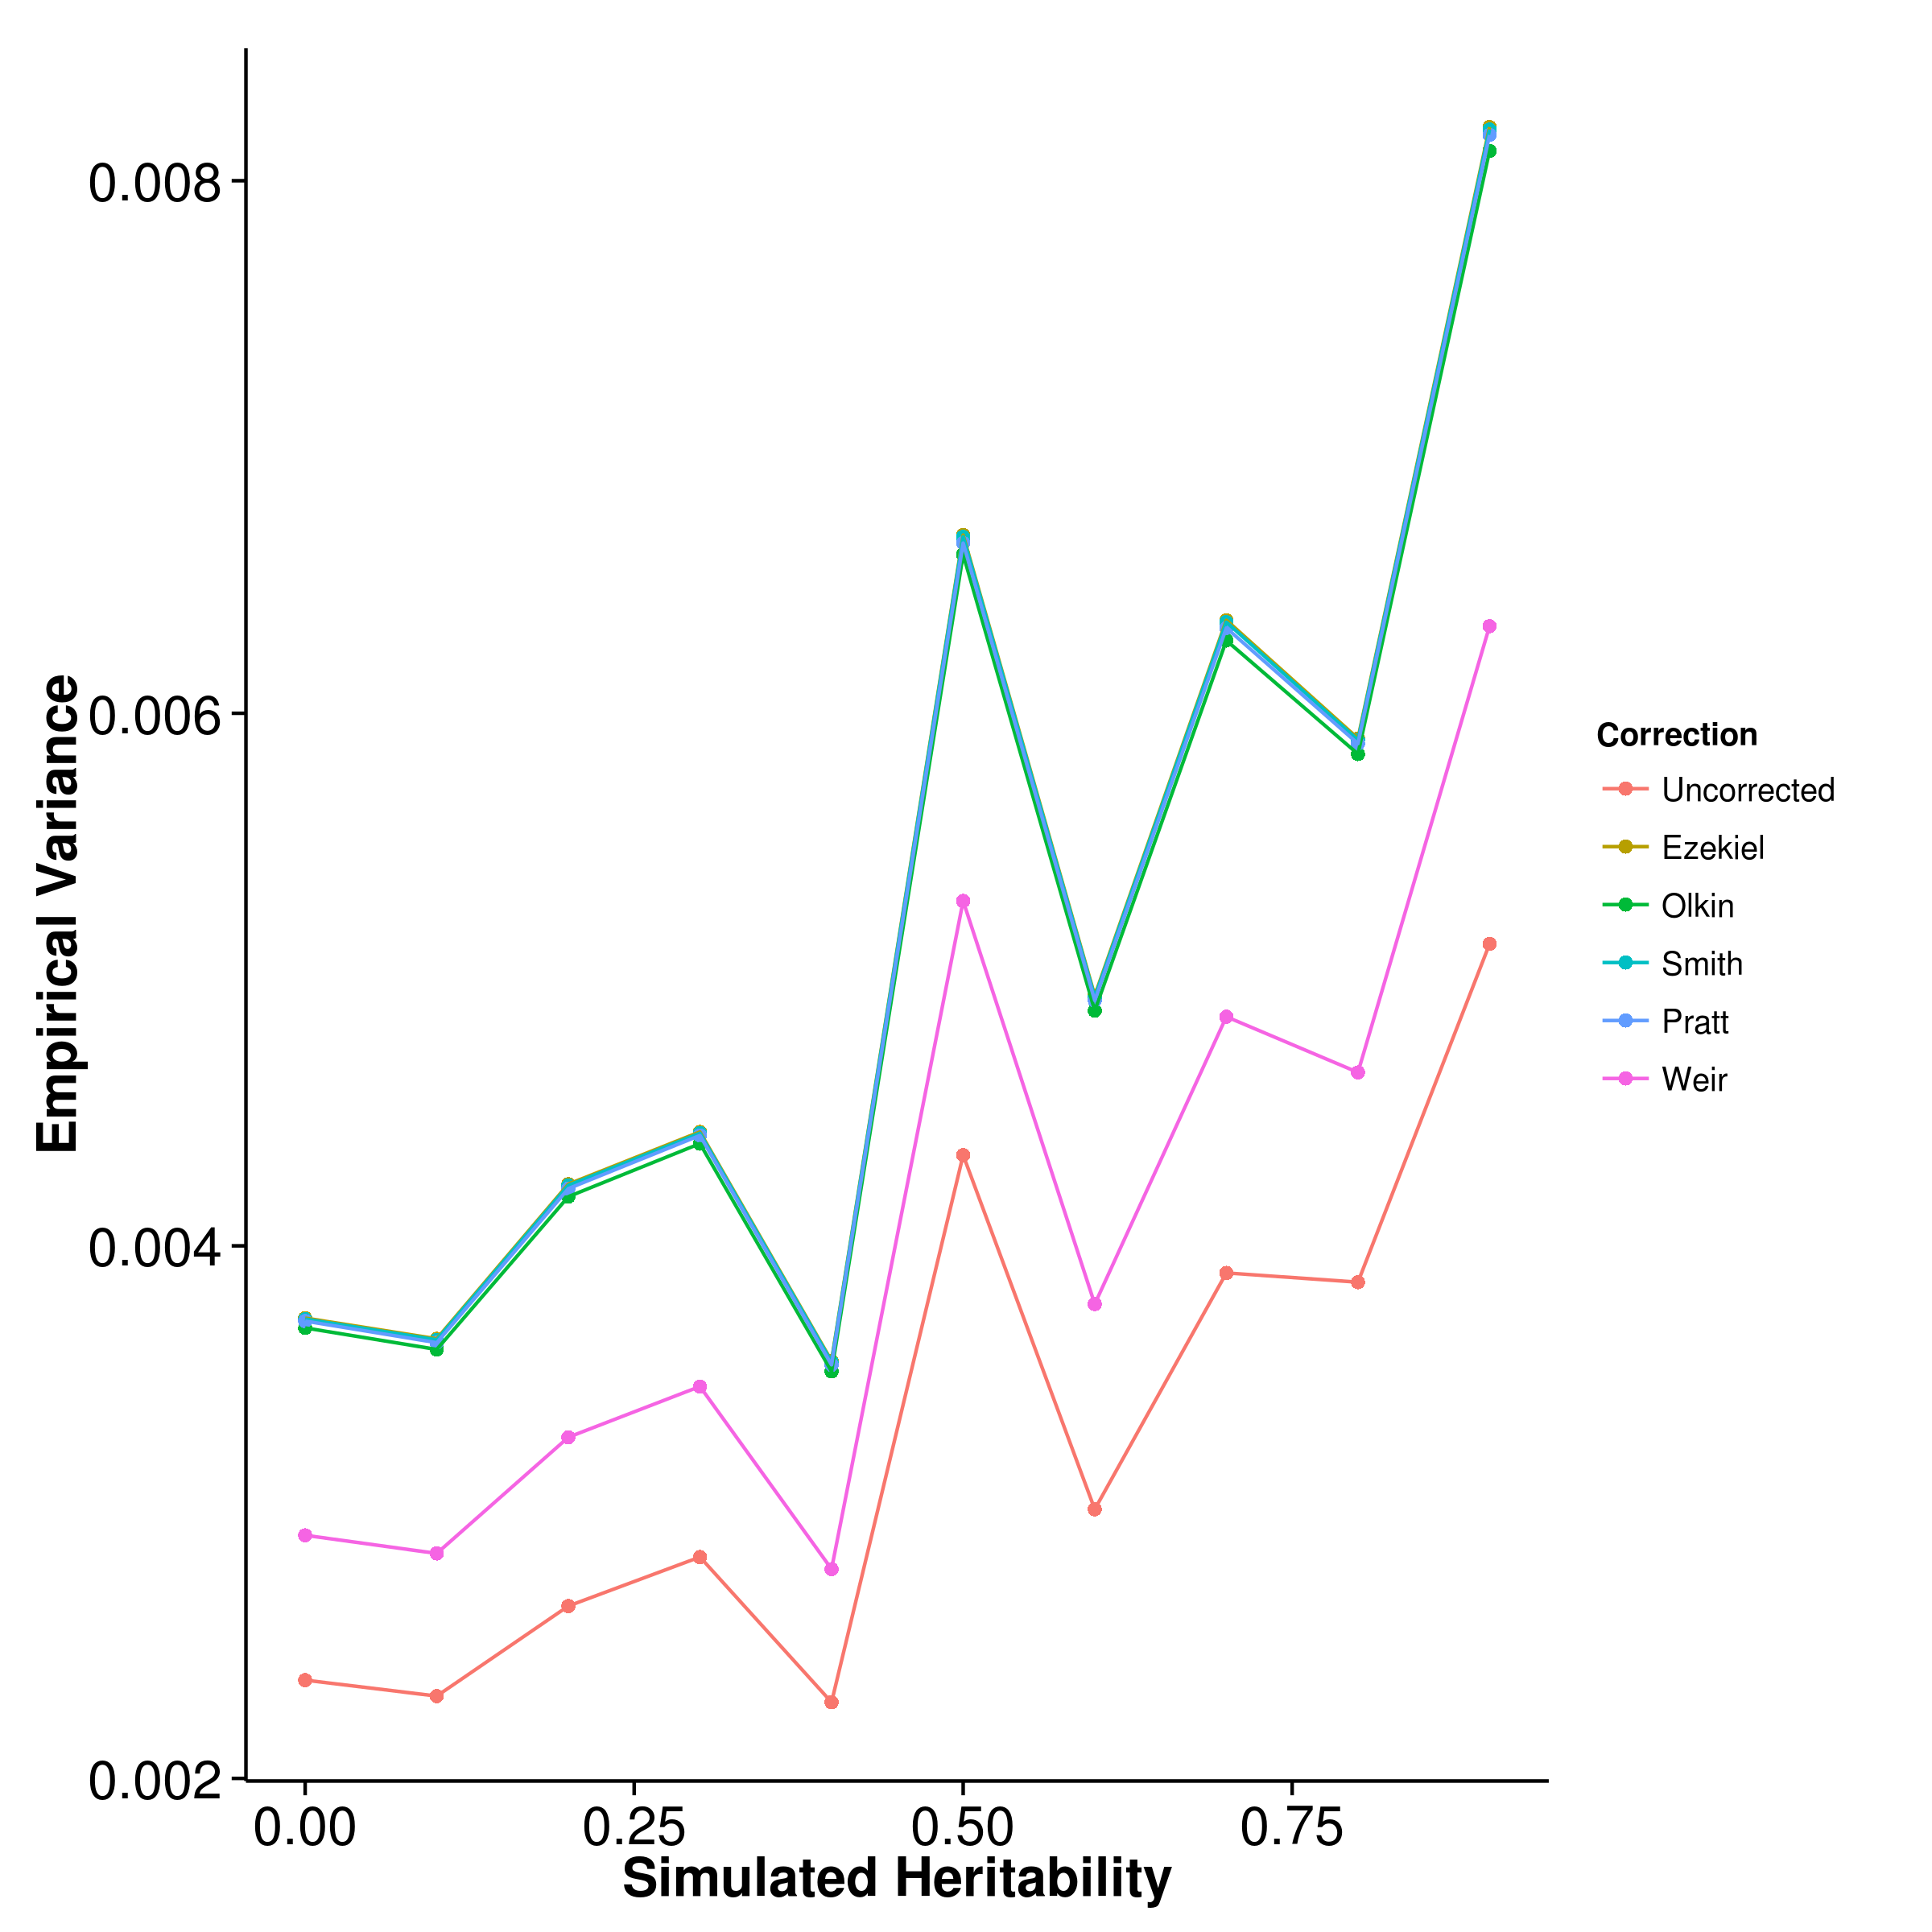
\includegraphics{figure/quantitative/ld_correct/ldCom_var.png}}
				\label{fig:varLDCor}
			}
			\caption[Effect of LD correction to Heritability Estimation]
			{Effect of LD correction to Heritability Estimation.
				We compared the performance of our algorithm when different $R^2$ bias correction algorithm was used.
				When no bias correction was carried out, a downward bias was observed. 
				After the application of the bias correction algorithms, the mean estimations of all except in the case of Weir \cref{eq:weir} algorithms leads to an overestimation of heritability.
				On the other hand, the corrections all lead to increase in variance of the estimation.
			} 
			\label{fig:ldCorCom}
		\end{figure}
		First, we would like to assess the effect of \gls{LD} correction on the heritability estimation and the impact of different bias correction algorithms. 
		By performing the simulation using HAPGEN2, we were able to simulate sample with \gls{LD} structure comparable to the \gls{LD} of the 1000 genome \gls{CEU} samples.
		
		First, we would like to compare the performance of \gls{shrek} when different bias correction algorithms were applied (\cref{fig:meanLDCor}).
		From the graph, it was observed that when no bias correction was applied, the mean estimation were in general downwardly biased.
		This was consistent with our expectation of a general upward bias in sample $R^2$ which will downwardly penalize the resulting heritability estimation.
		On the other hand, the bias correction algorithms all worked as expected where they increases the mean estimation of heritability.
		By removing the upward bias in the sample $R^2$, the heritability estimation should increase.
		However for most algorithms except for Weir's formula (\cref{eq:weir}) an over adjustment were observed, leading to a general upward bias in the estimation.
		Taking into account of the variance of estimation (\cref{fig:varLDCor}), Weir's formula were the most suitable for \gls{shrek} where not only it reduces the bias in the final heritability estimation, it does not introduce too much additional variance into the estimation.
		As a result of that, we selected the Weir's formula as our default \gls{LD} correction algorithm.
		
		\subsection{Comparing with Other Algorithms}
		Having selected the optimal \gls{LD} correction algorithm, we then compared the performance of \gls{shrek} with existing algorithms to understand the relative of these algorithms under different conditions.
		First, we examined the performance of the algorithms under the quantitative trait scenario where we varies the trait heritability and the number of causal \glspl{SNP}.
		\subsubsection{Quantitative Trait Simulation}
			\begin{figure}
			\centering
			\subfloat[SHREK]{
				\scalebox{.4}{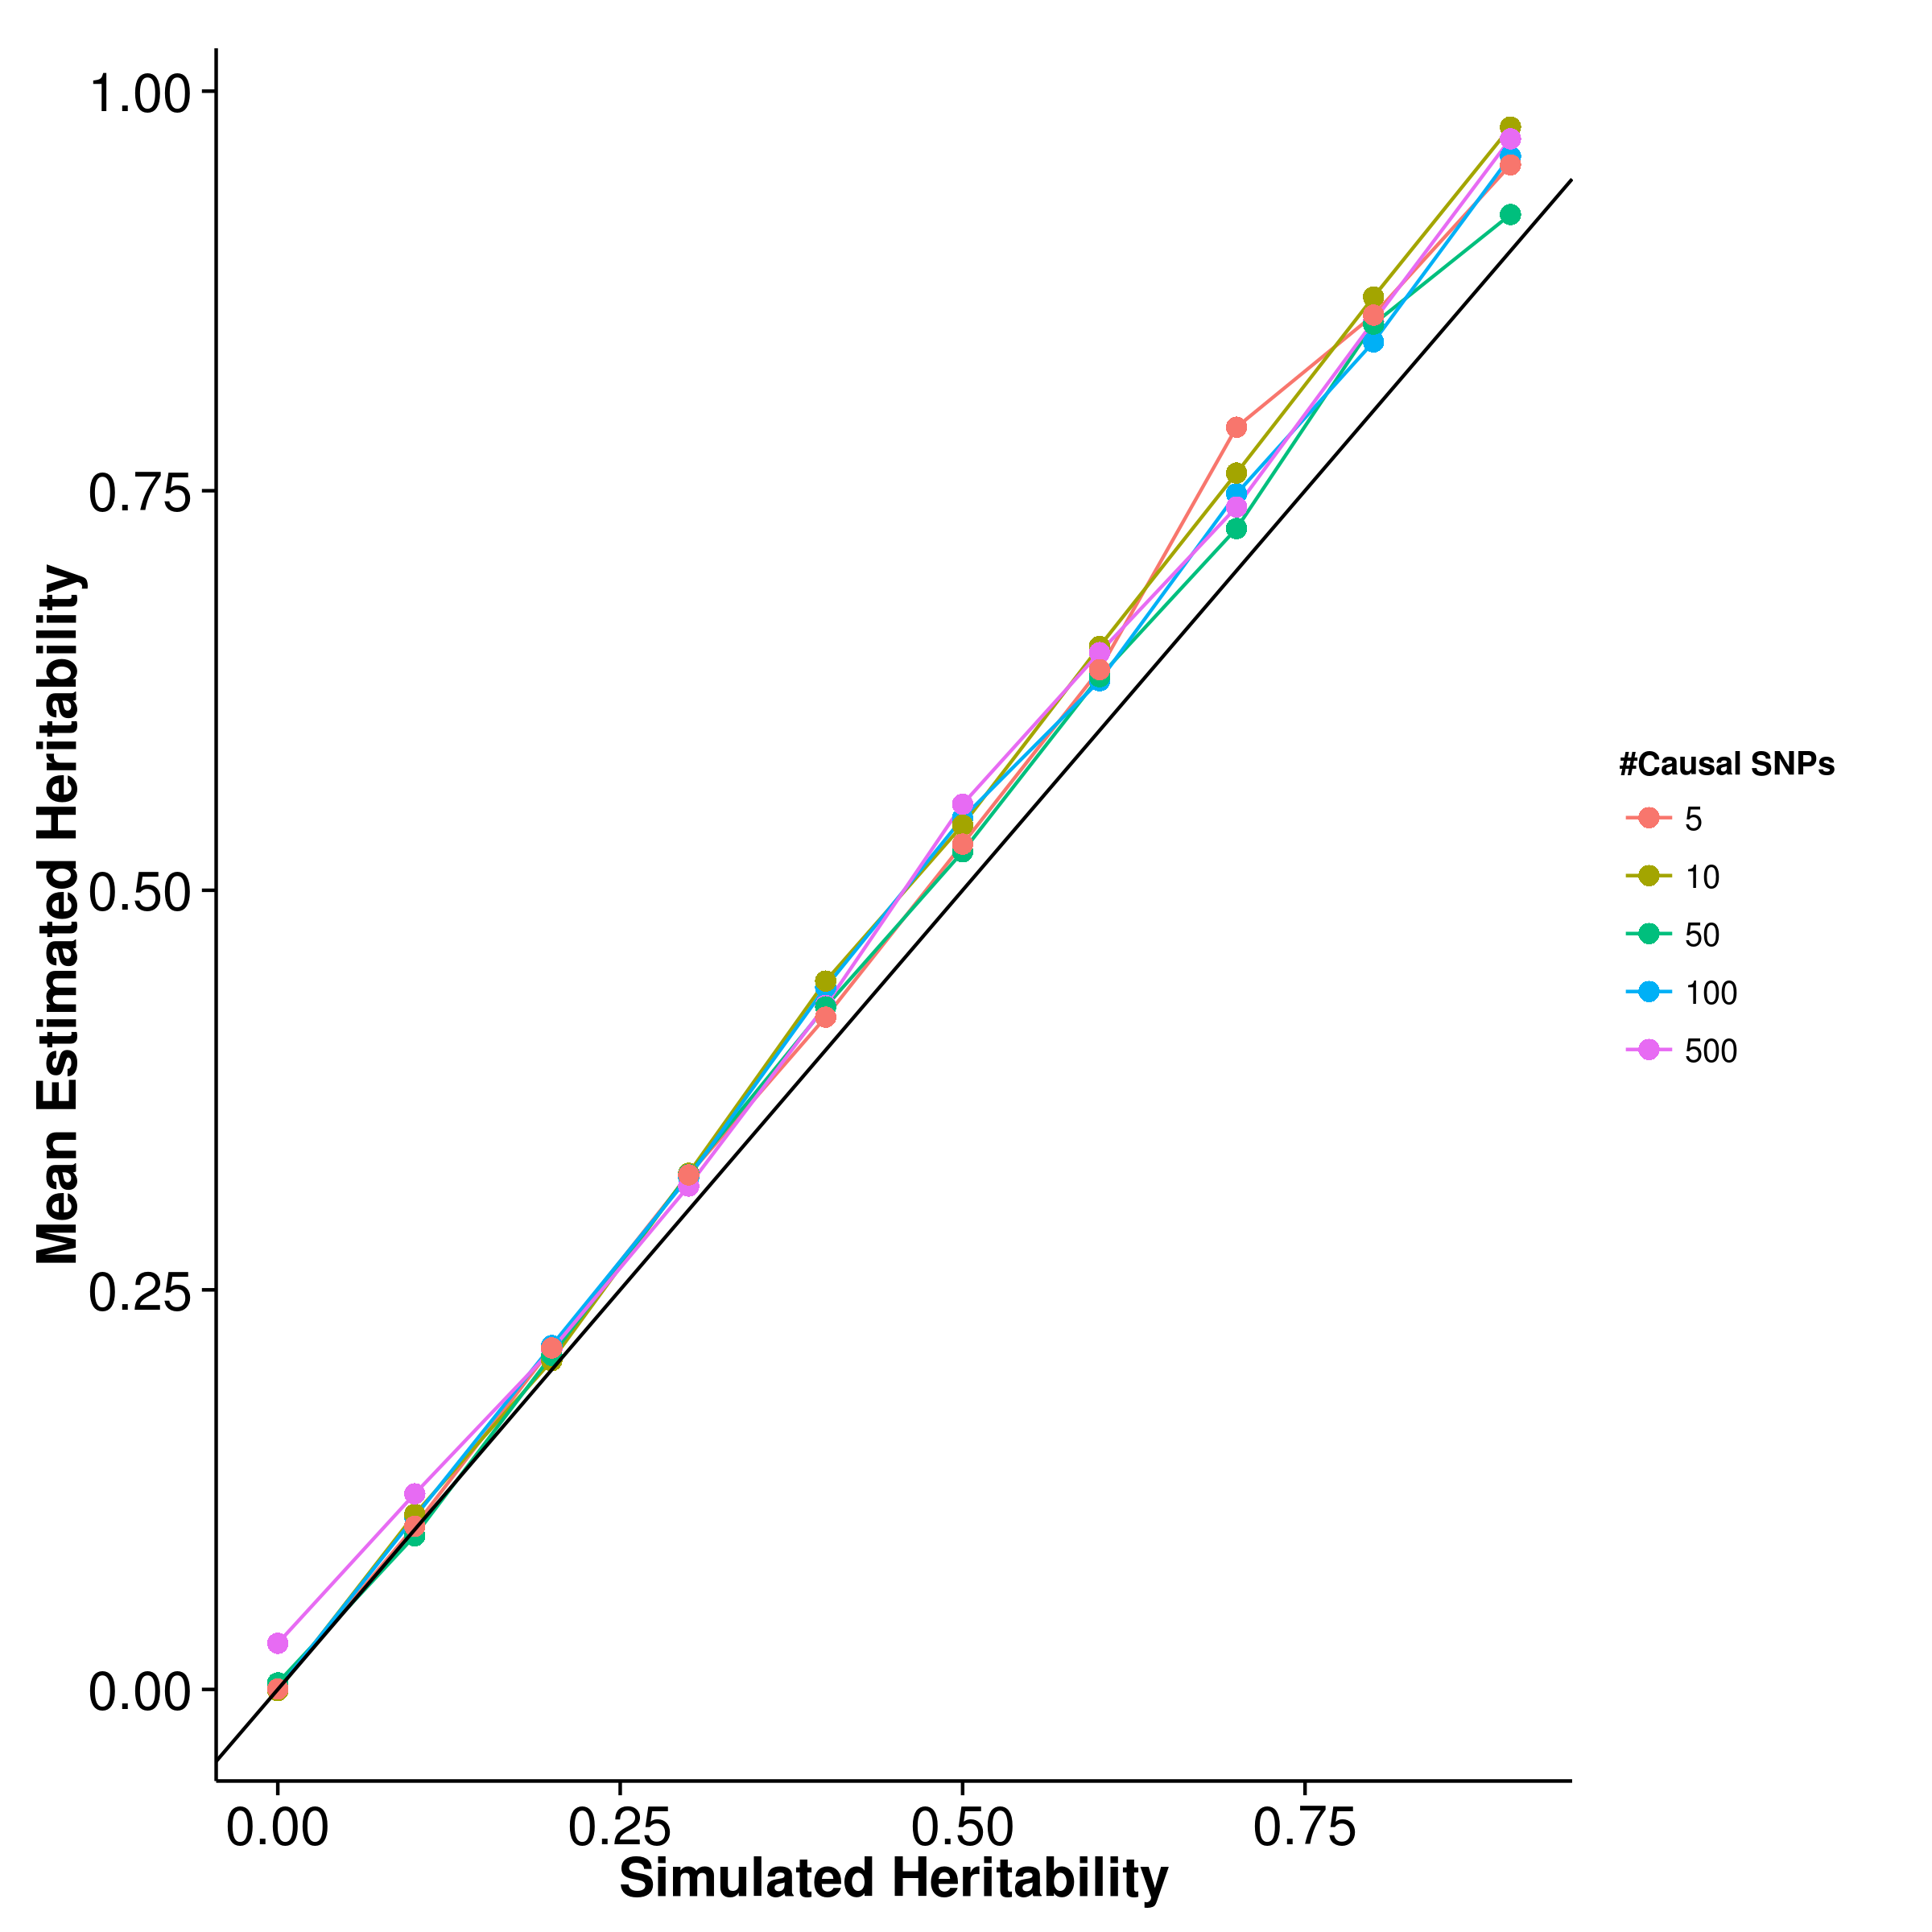
\includegraphics{figure/he_summary/random/shrek_Qt_Rand_mean.png}}
				\label{fig:shrekQtRandMean}
			}
			\subfloat[GCTA]{
				\scalebox{.4}{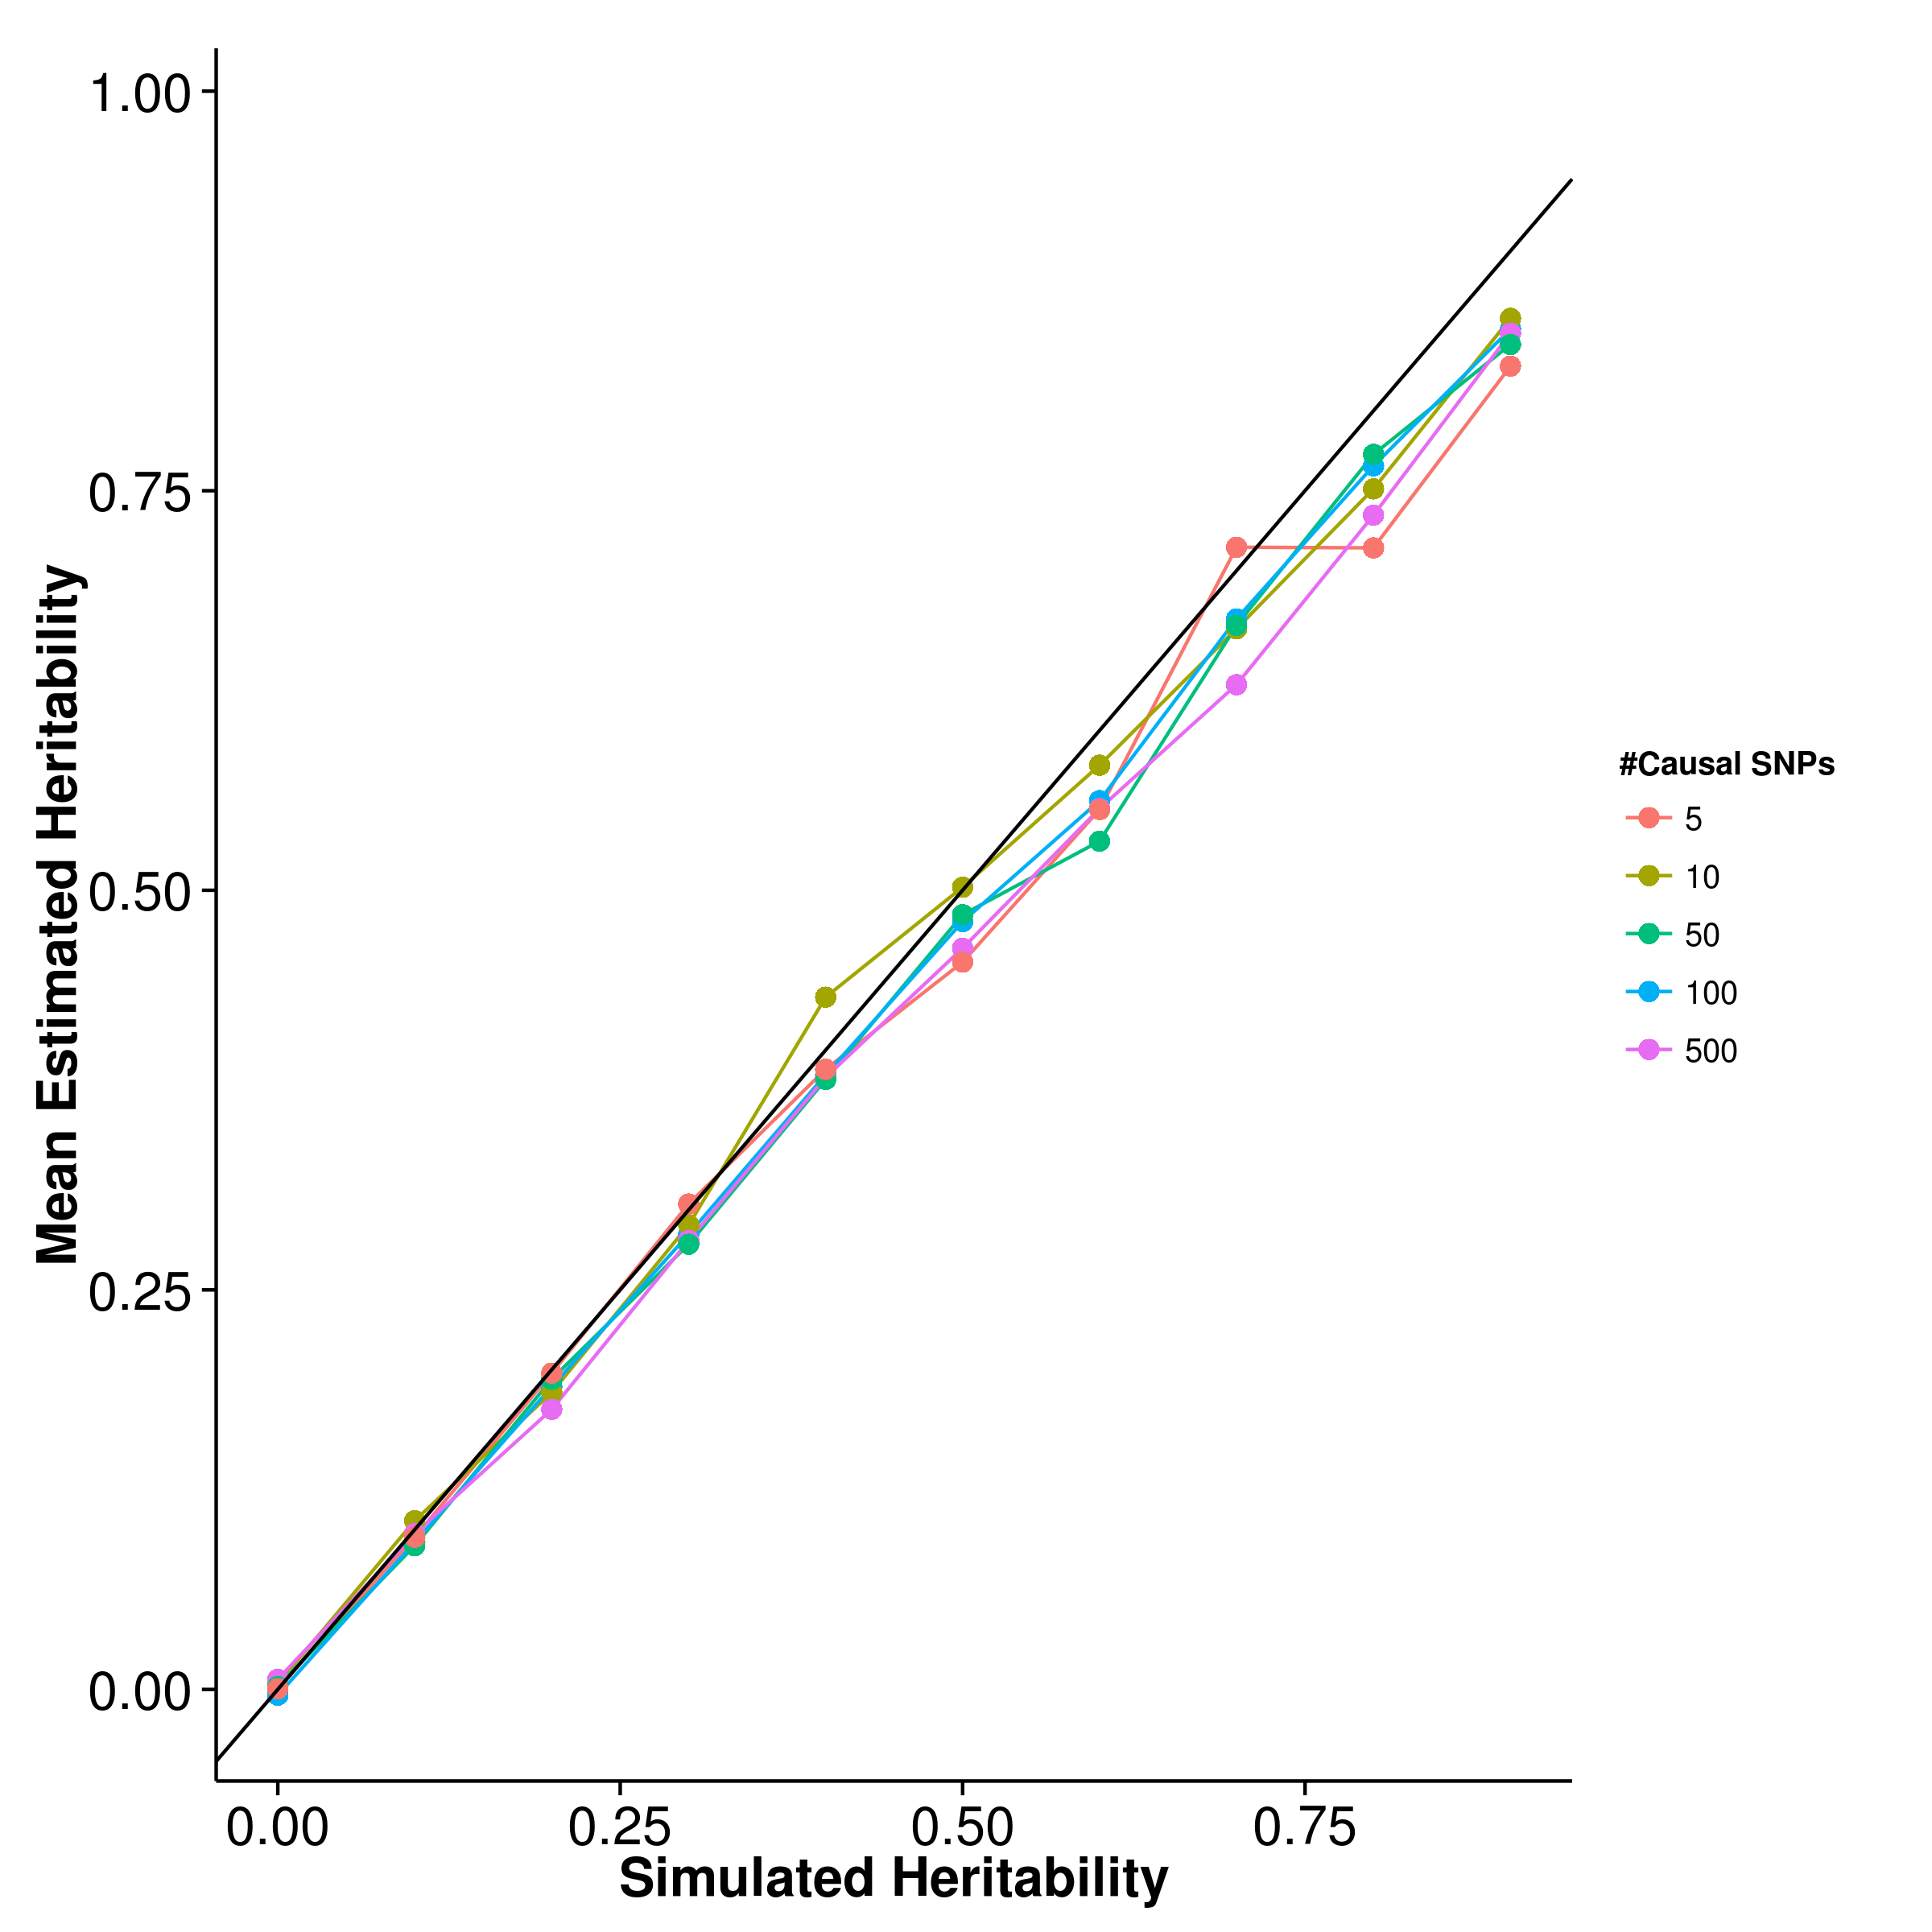
\includegraphics{figure/he_summary/random/gcta_Qt_Rand_mean.png}}
				\label{fig:gctaQtRandMean}
			}\\
			\subfloat[LDSC with fix intercept]{
				\scalebox{.4}{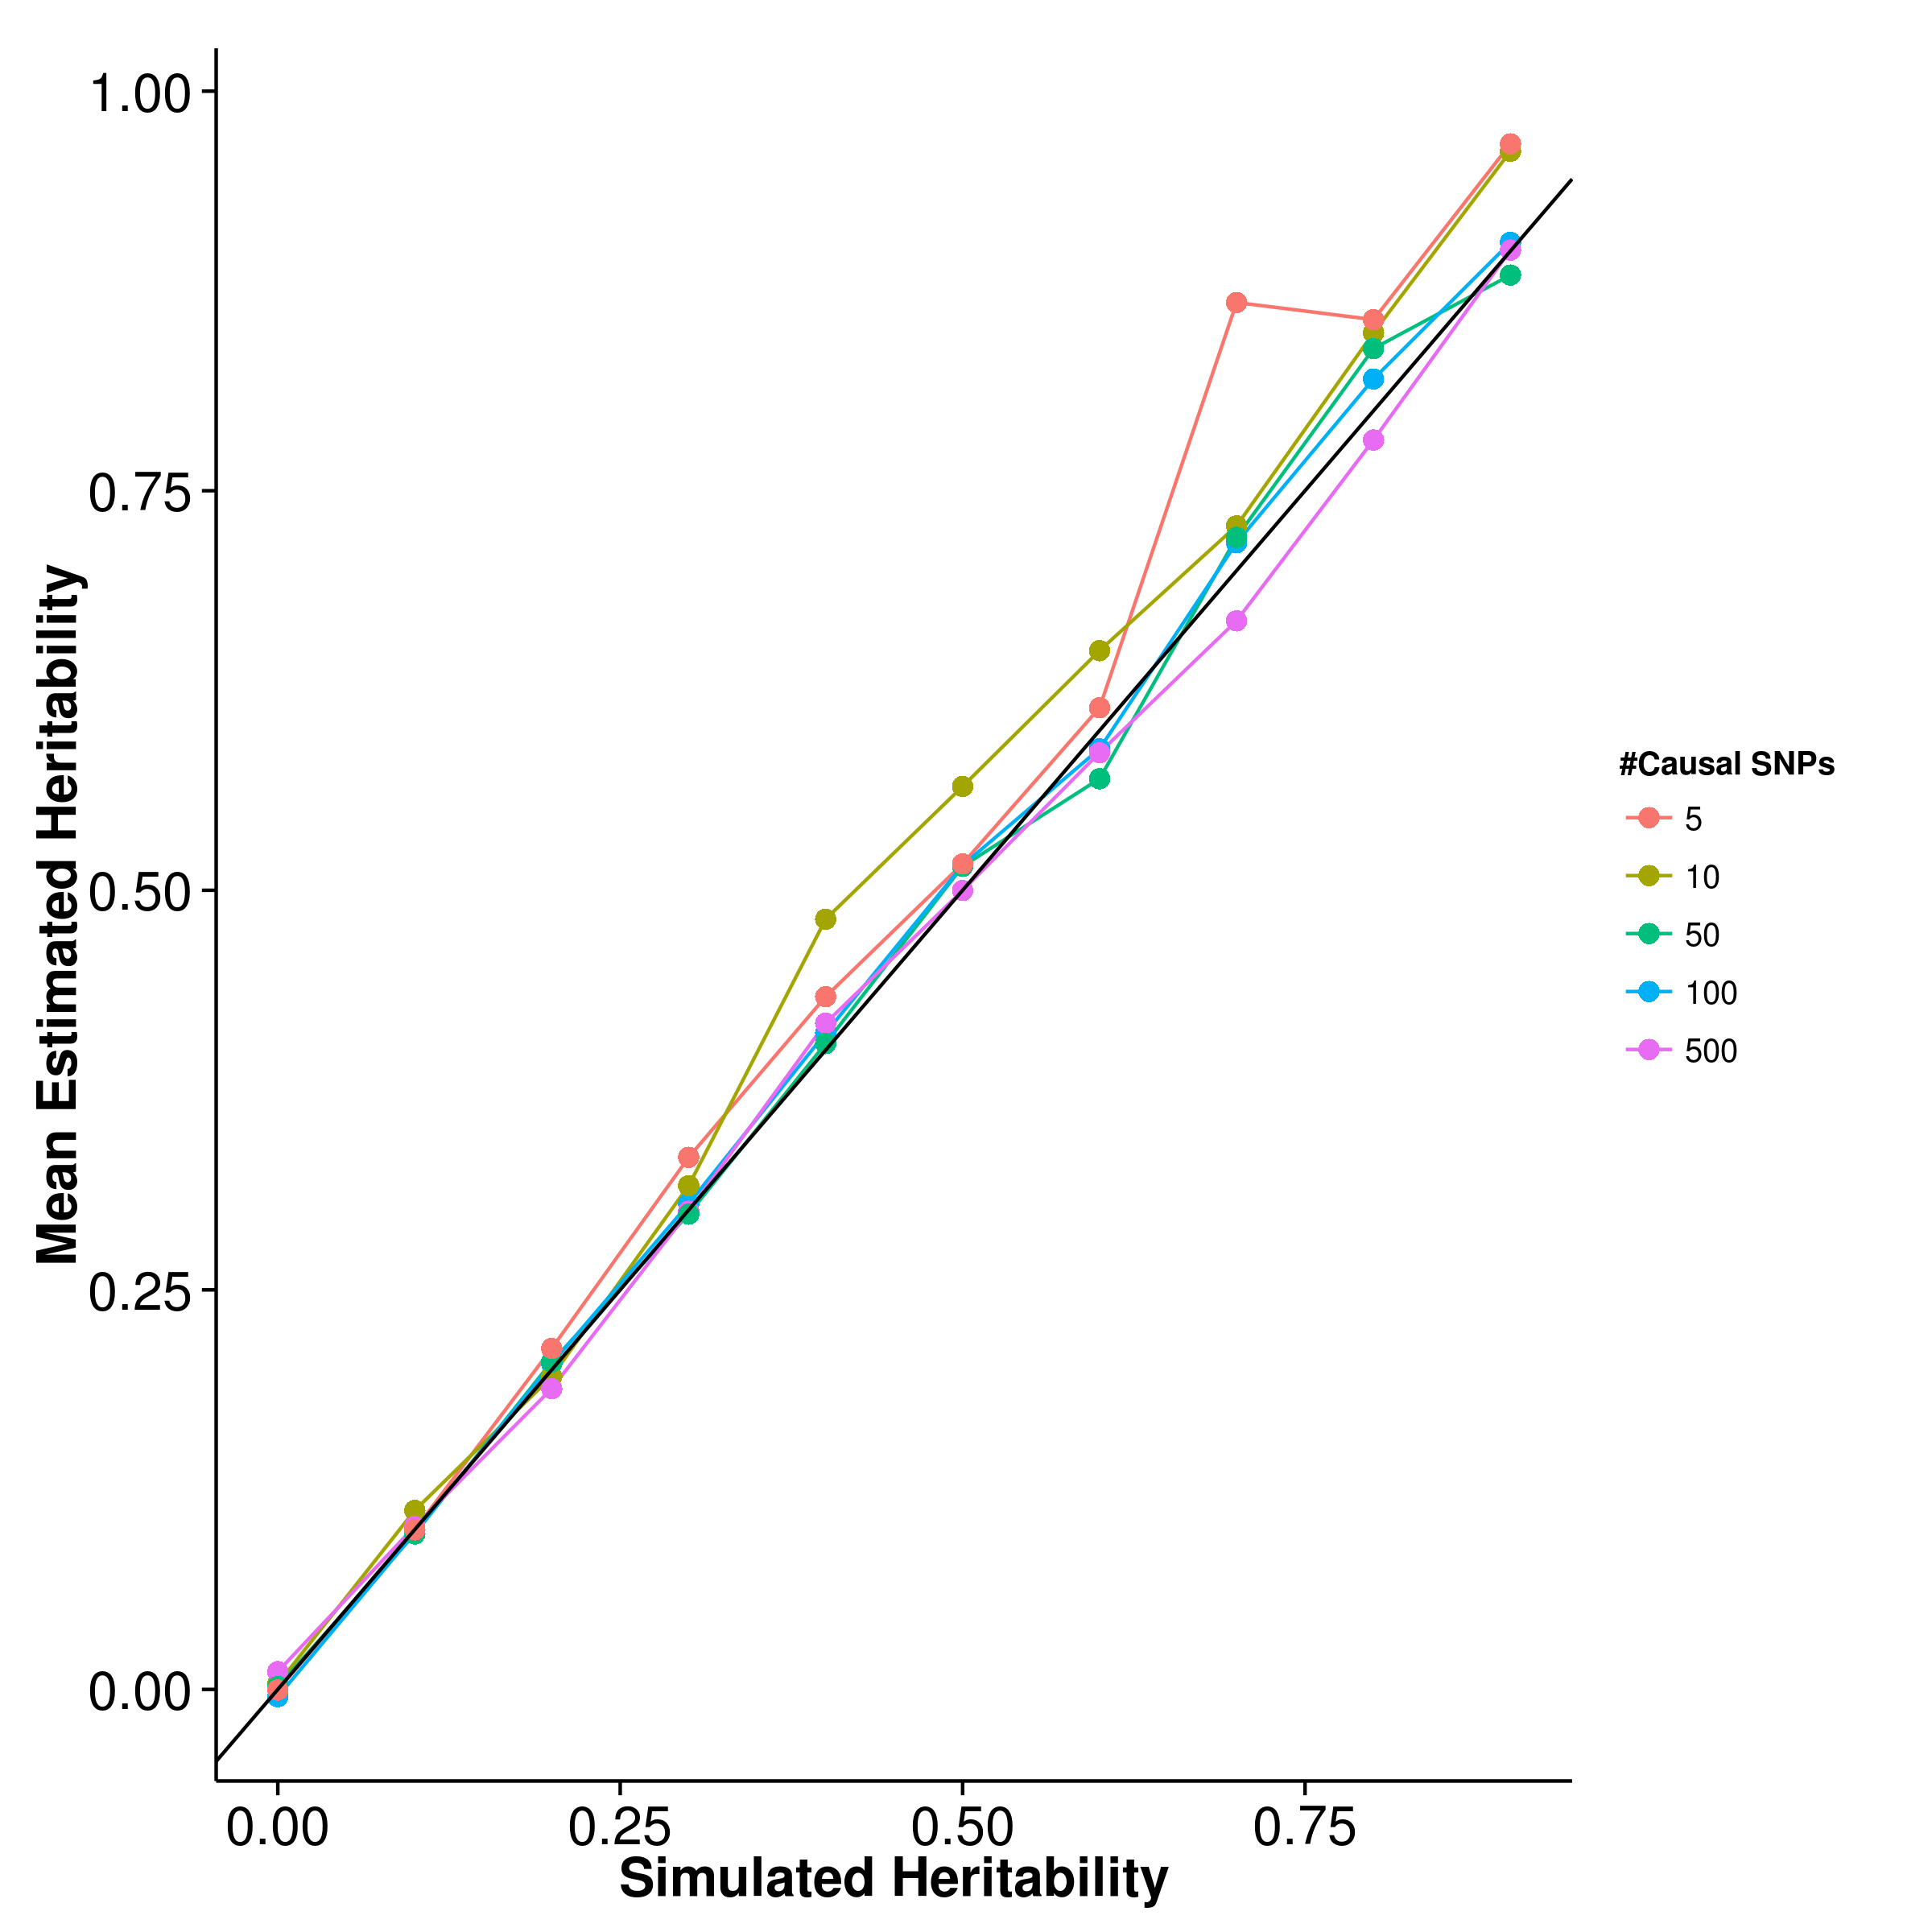
\includegraphics{figure/he_summary/random/ldsc_Qt_Rand_mean.png}}
				\label{fig:ldscQtRandMean}
			}
			\subfloat[LDSC with intercept estimation]{
				
				\scalebox{.4}{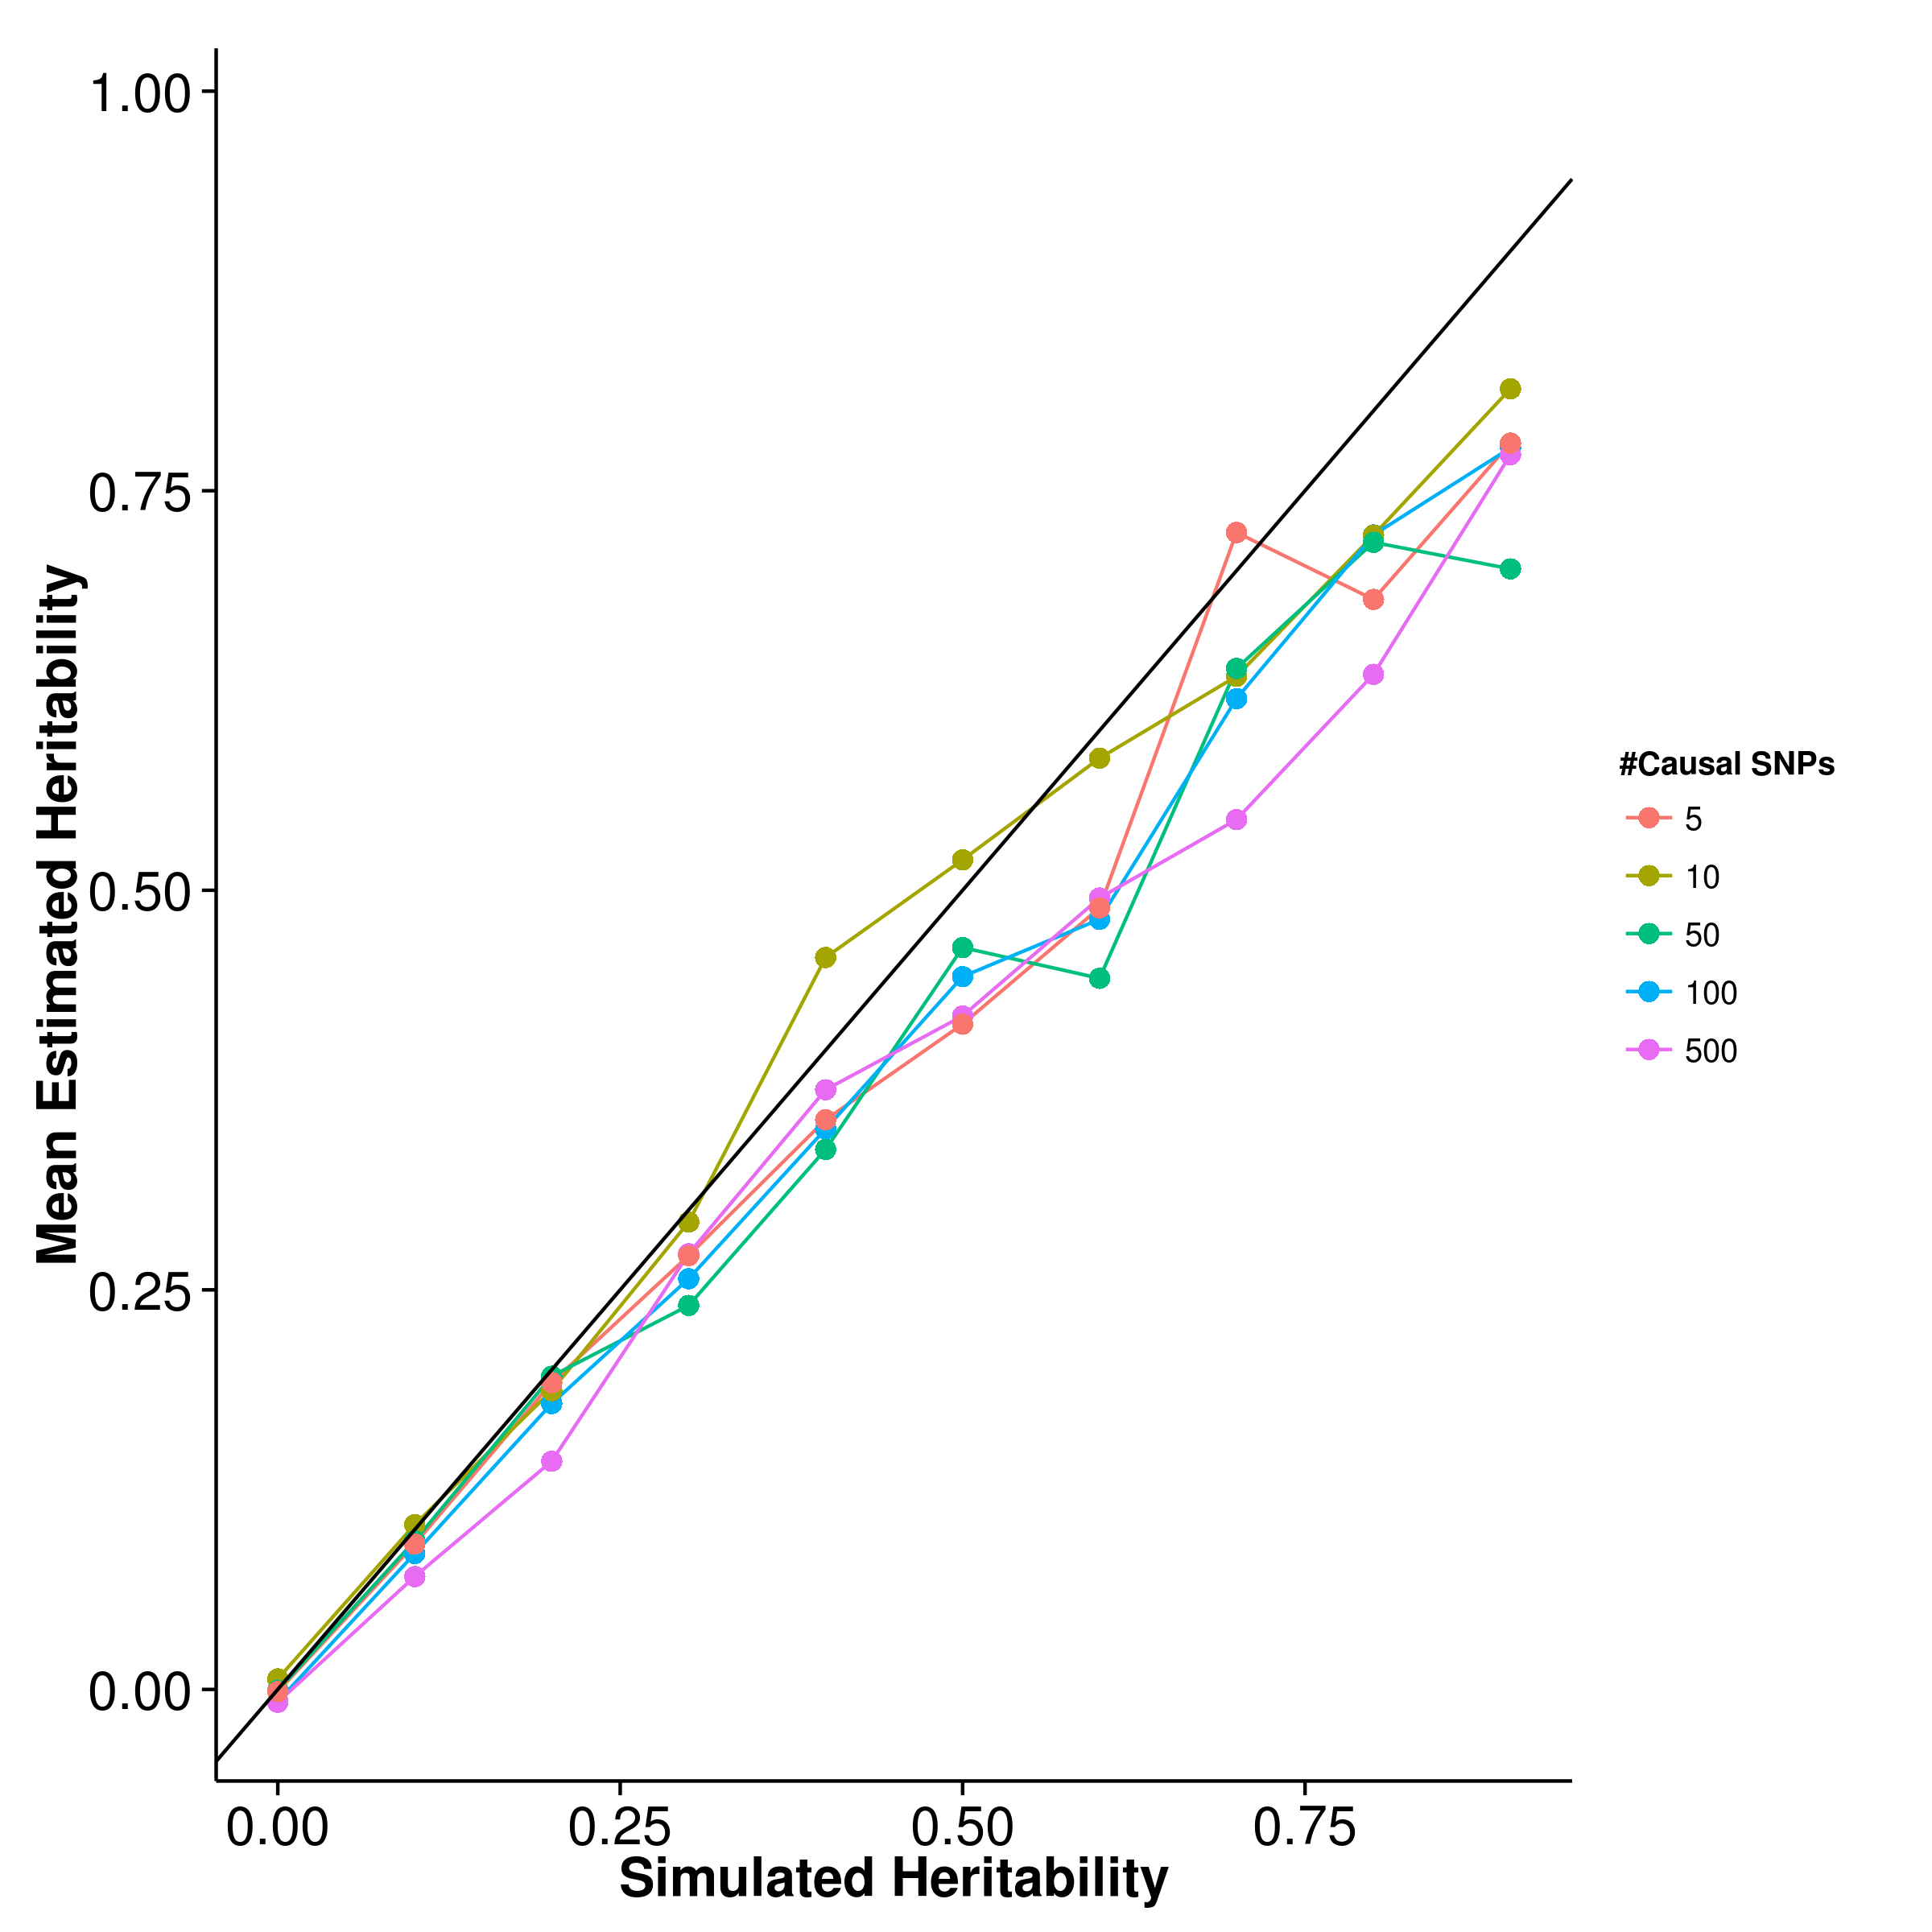
\includegraphics{figure/he_summary/random/ldscIn_Qt_Rand_mean.png}}
				\label{fig:ldscInQtRandMean}
			}
			\caption[Mean of Quantitative Trait Simulation Results]
			{Mean of results from quantitative trait simulation with random effect size simulation.
				Estimations form \gls{shrek} were slightly biased upwards whereas \gls{gcta} and \gls{ldsc} with intercept estimations both biased downwards.
				On the other hand, \gls{ldsc} with fixed intercept provides least biased estimates under polygenic conditions. 
				However, when the number of causal \glspl{SNP} is small (e.g. 5 or 10), an upward bias was observed.} 
			\label{fig:QtRandMean}
		\end{figure}
		
		\begin{figure}
			\centering
			\subfloat[SHREK]{
				\scalebox{.4}{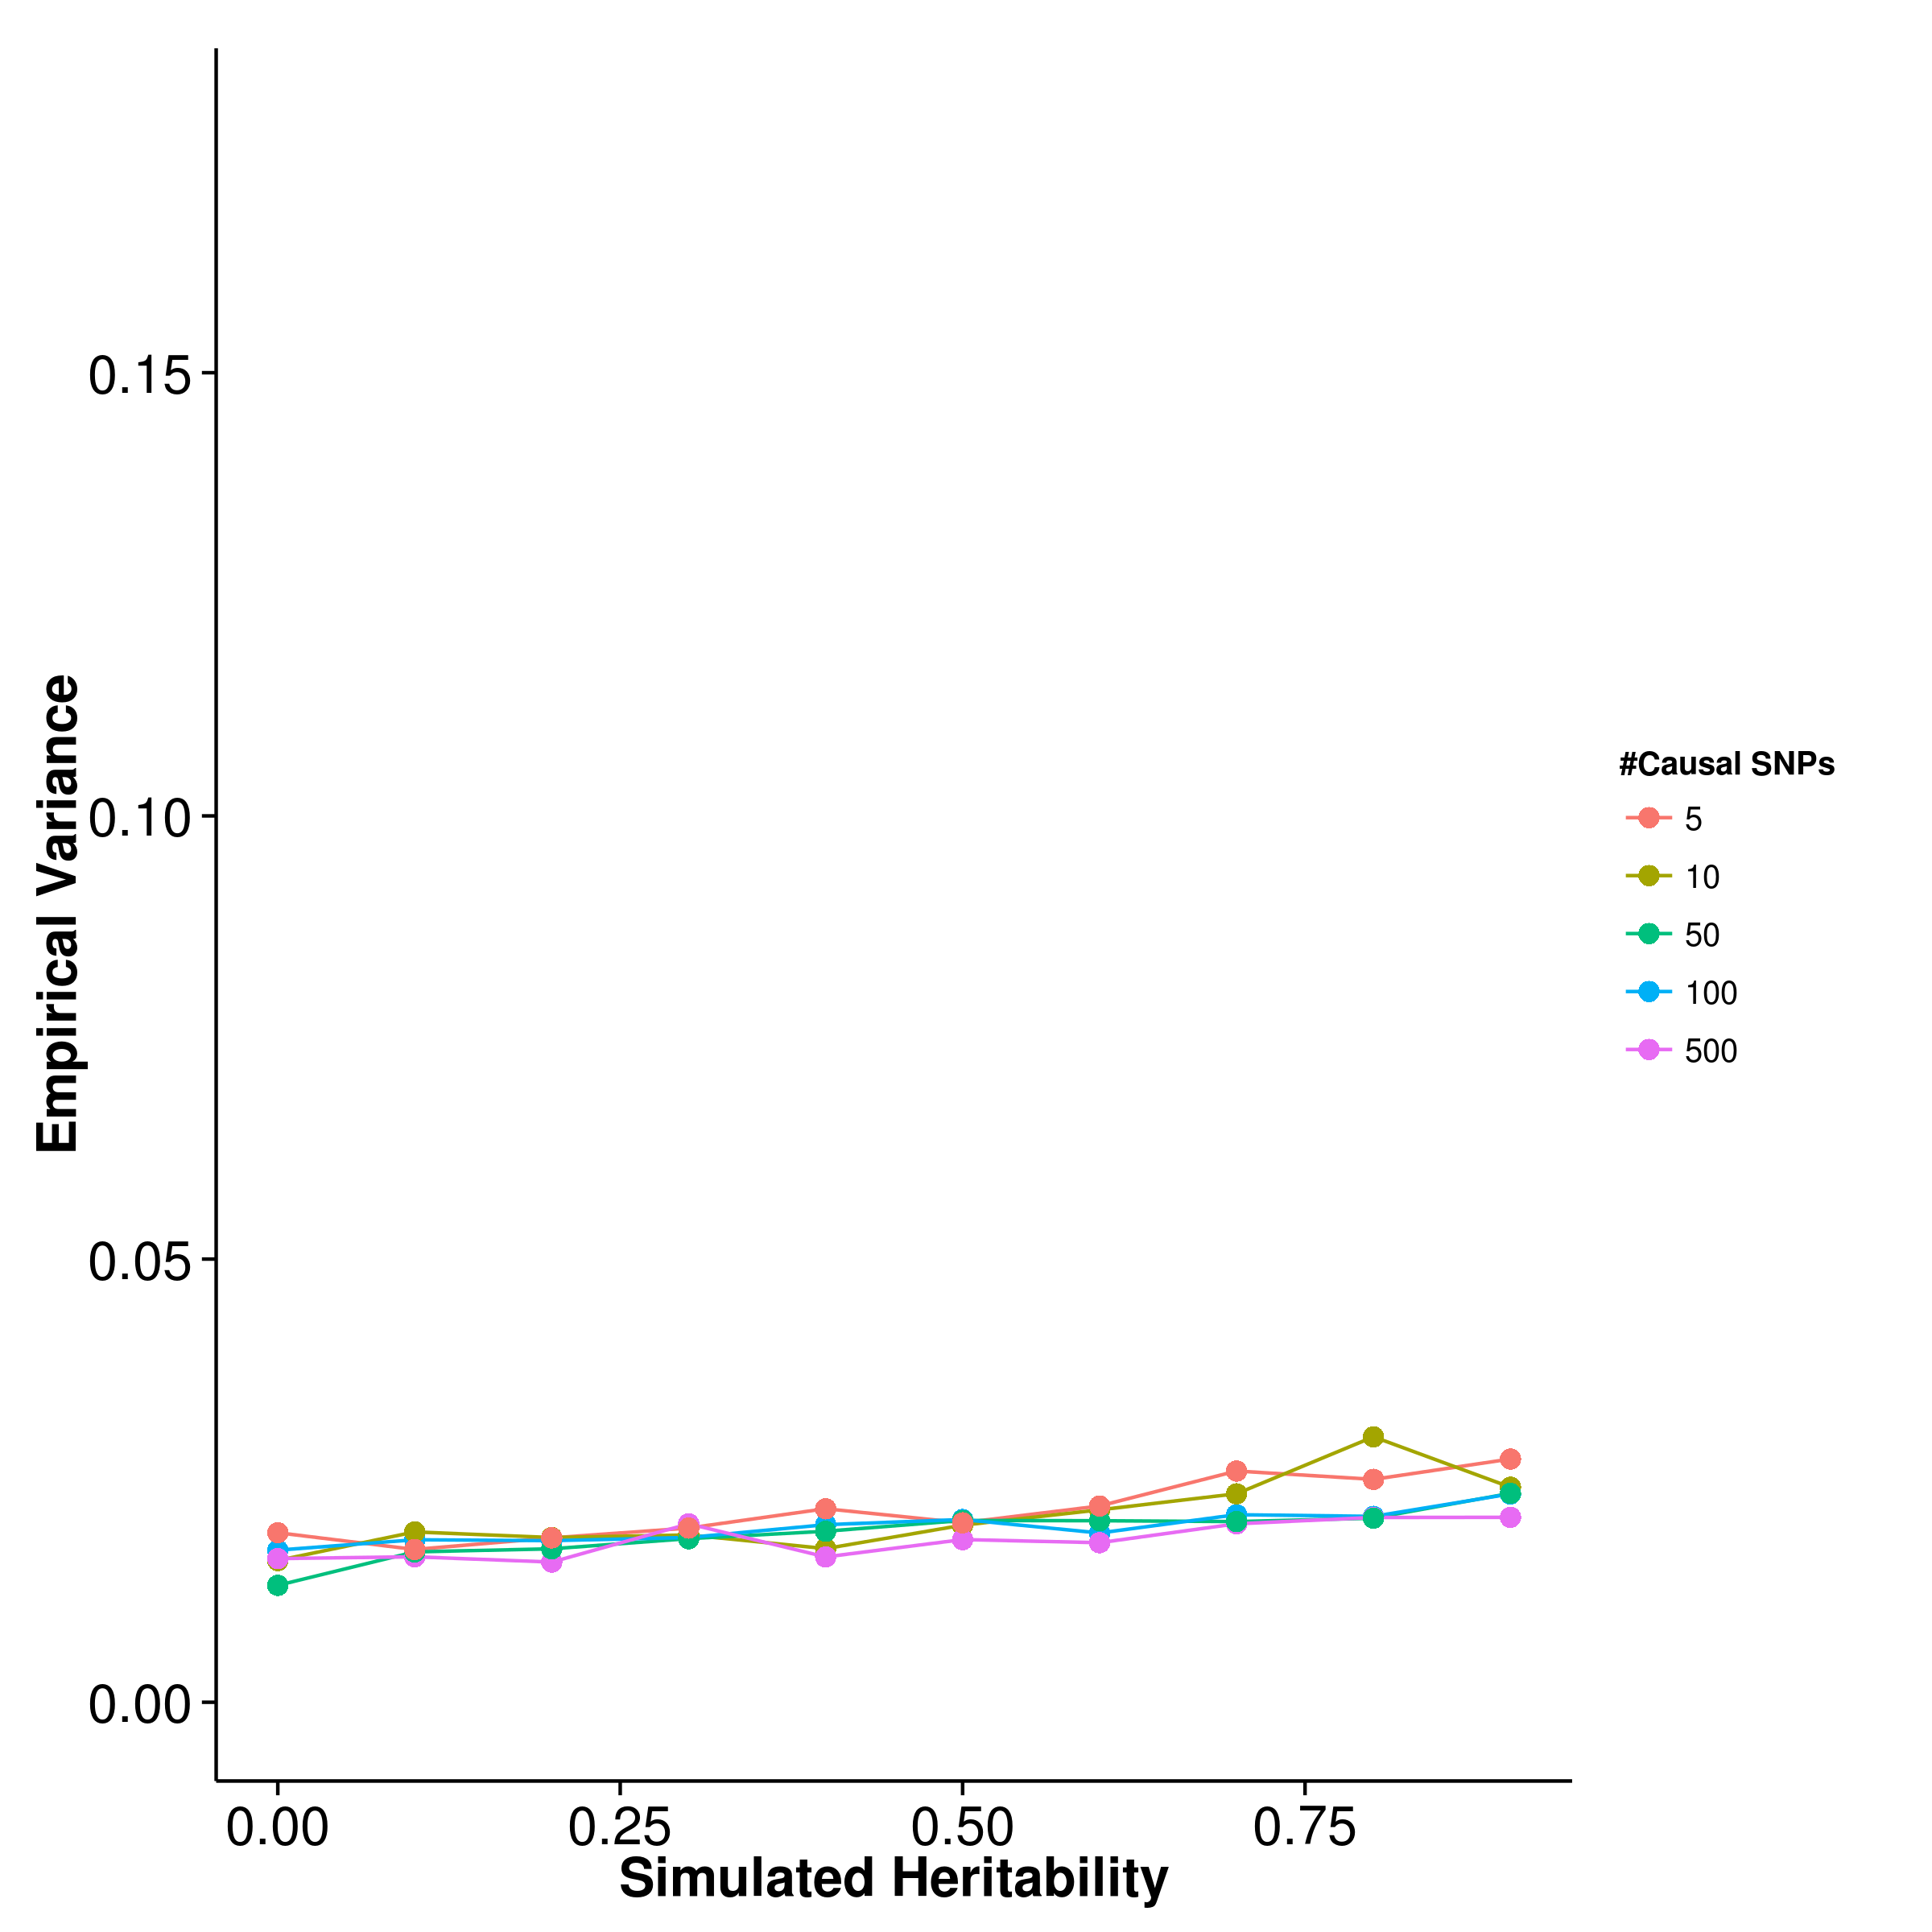
\includegraphics{figure/he_summary/random/shrek_Qt_Rand_sd.png}}
				\label{fig:shrekQtRandVar}
			}
			\subfloat[GCTA]{
				\scalebox{.4}{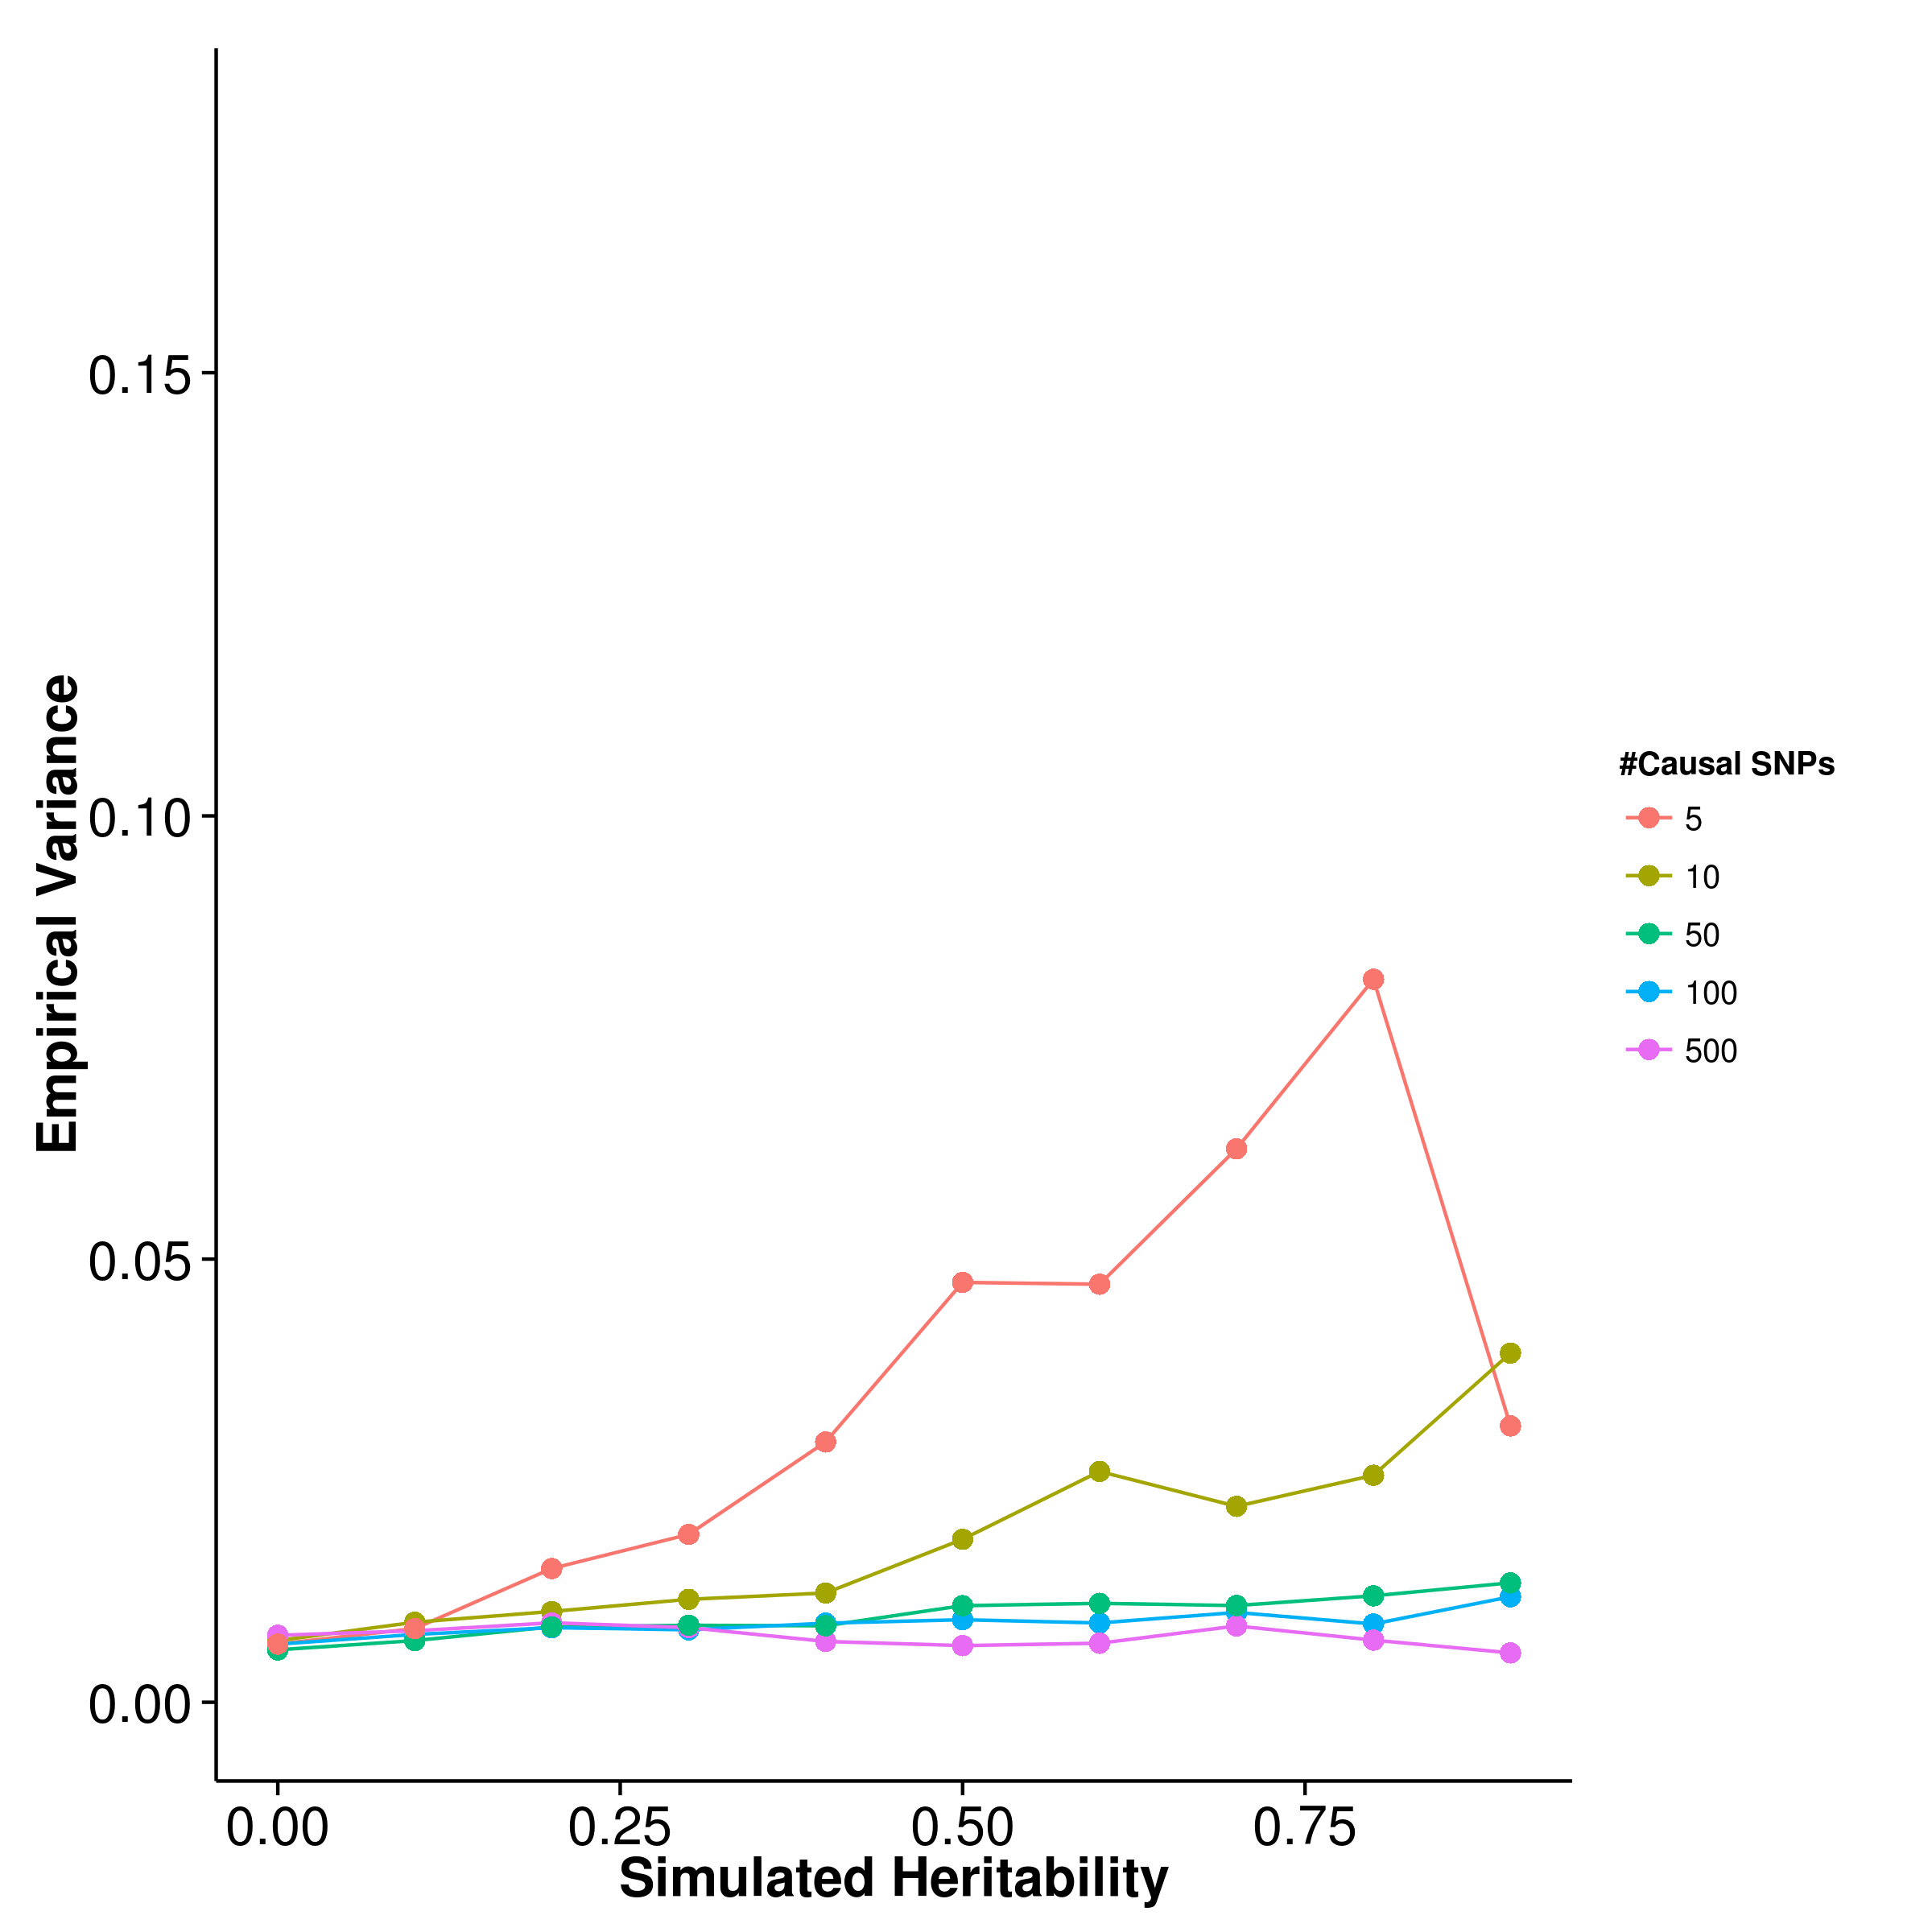
\includegraphics{figure/he_summary/random/gcta_Qt_Rand_sd.png}}
				\label{fig:gctaQtRandVar}
			}\\
			\subfloat[LDSC with fix intercept]{
				\scalebox{.4}{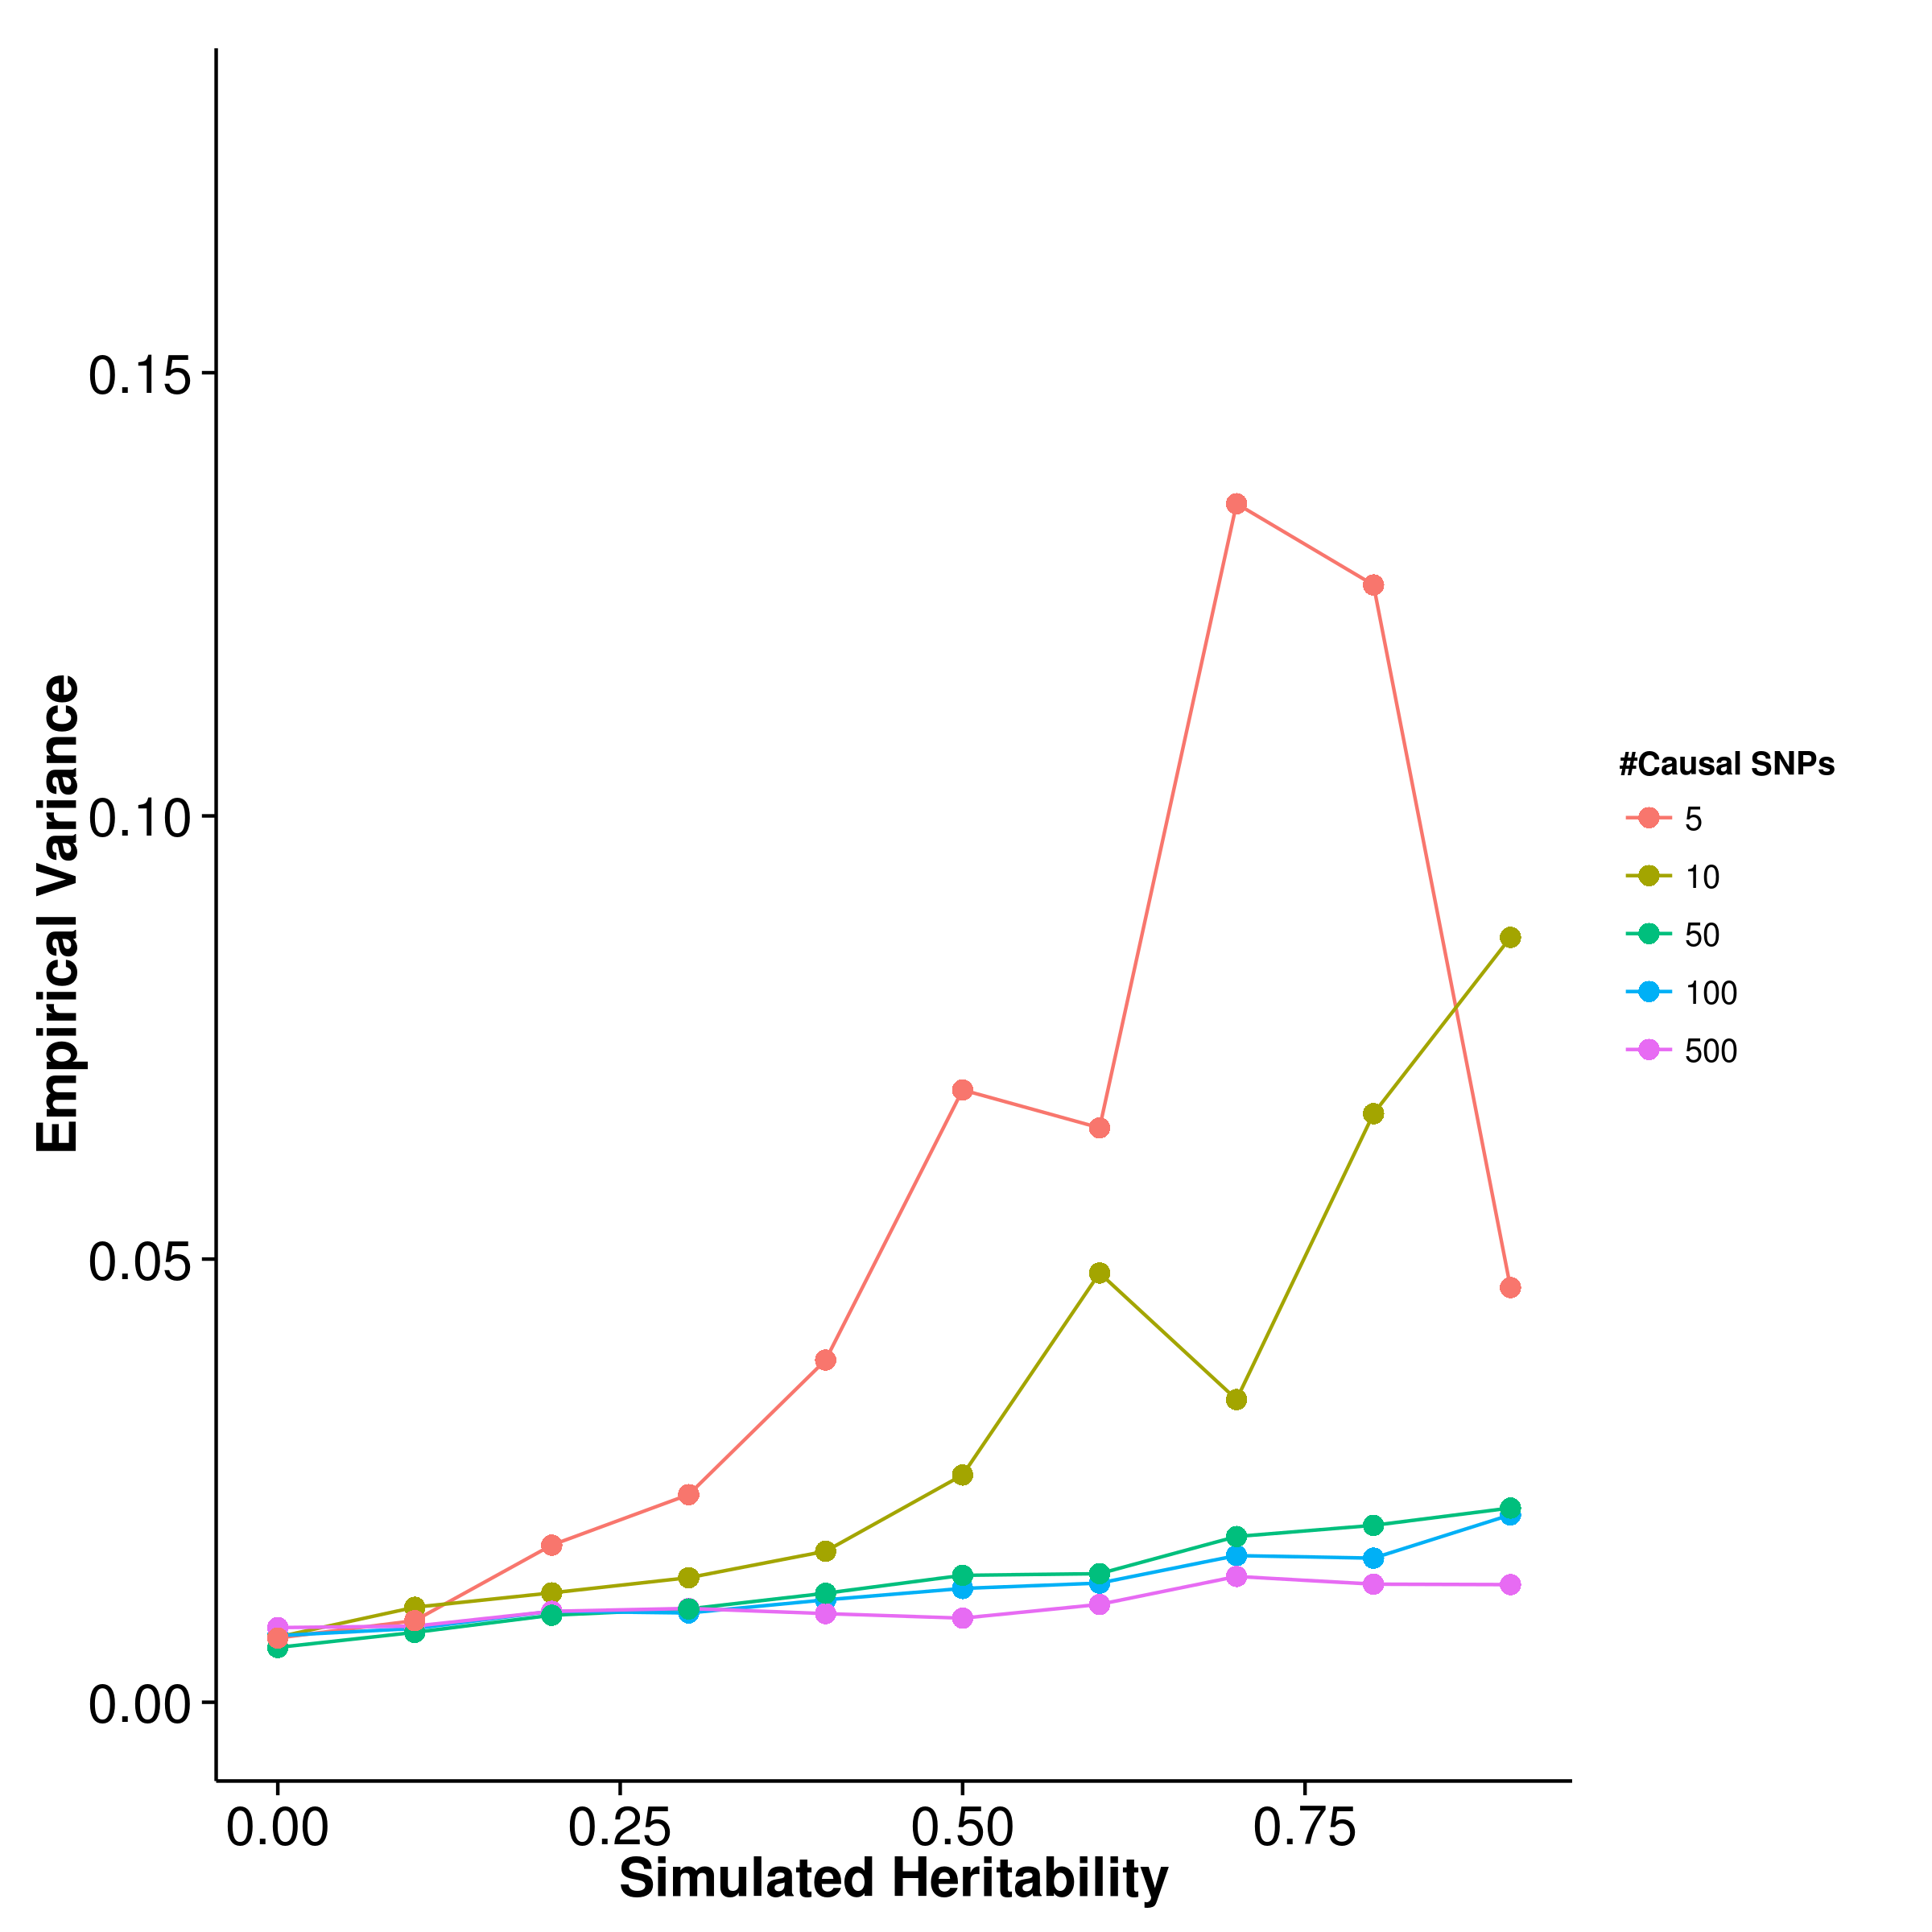
\includegraphics{figure/he_summary/random/ldsc_Qt_Rand_sd.png}}
				\label{fig:ldscQtRandVar}
			}
			\subfloat[LDSC with intercept estimation]{
				
				\scalebox{.4}{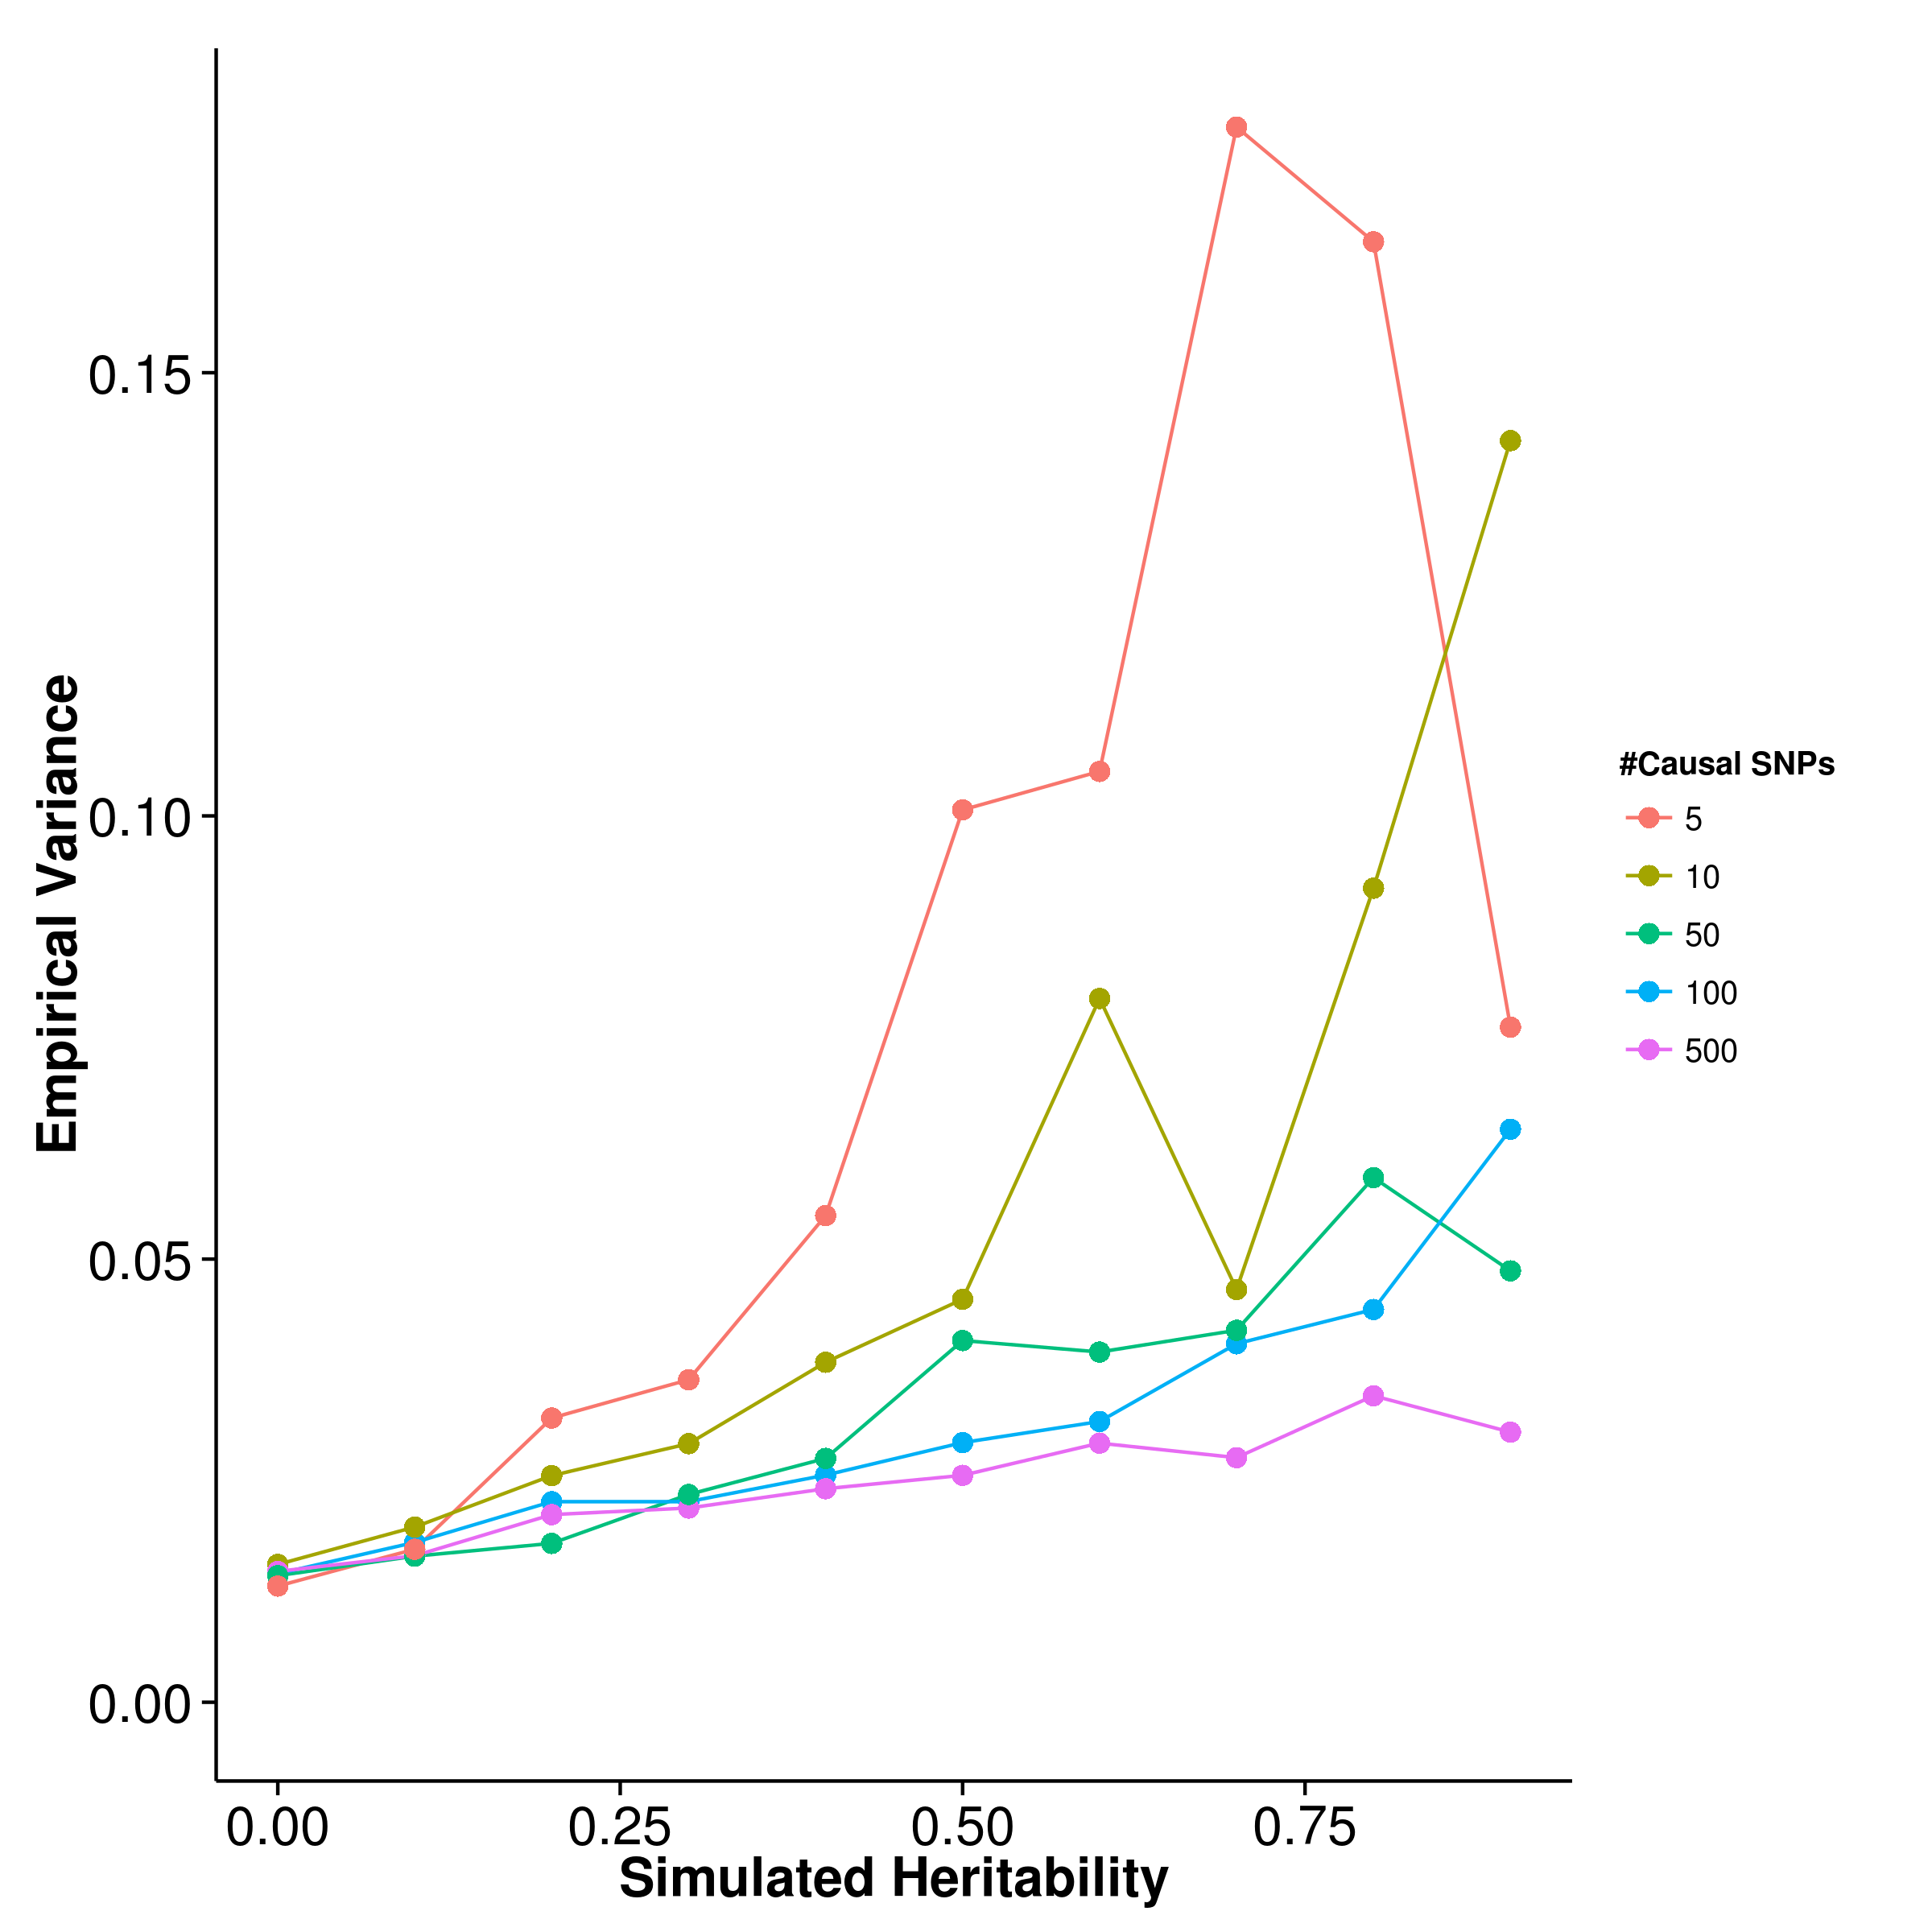
\includegraphics{figure/he_summary/random/ldscIn_Qt_Rand_sd.png}}
				\label{fig:ldscInQtRandVar}
			}
			\caption[Variance of Quantitative Trait Simulation Results]
			{Variance of results from quantitative trait simulation with random effect size simulation.
				Under the polygenic conditions, \gls{gcta} has the smallest variance, follow by \gls{ldsc}. 
				However, it was observed when the number of causal \glspl{SNP} decreases, the variance of the estimation increases for all algorithm, with variance of the \gls{shrek} estimate being the least affected.
				In fact, under oligogenic conditions, \gls{shrek} has a lower empirical variance when compared to \gls{ldsc}.
			} 
			\label{fig:QtRandVar}
		\end{figure}
		
		\begin{figure}
			\centering
			\subfloat[SHREK]{
				\scalebox{.4}{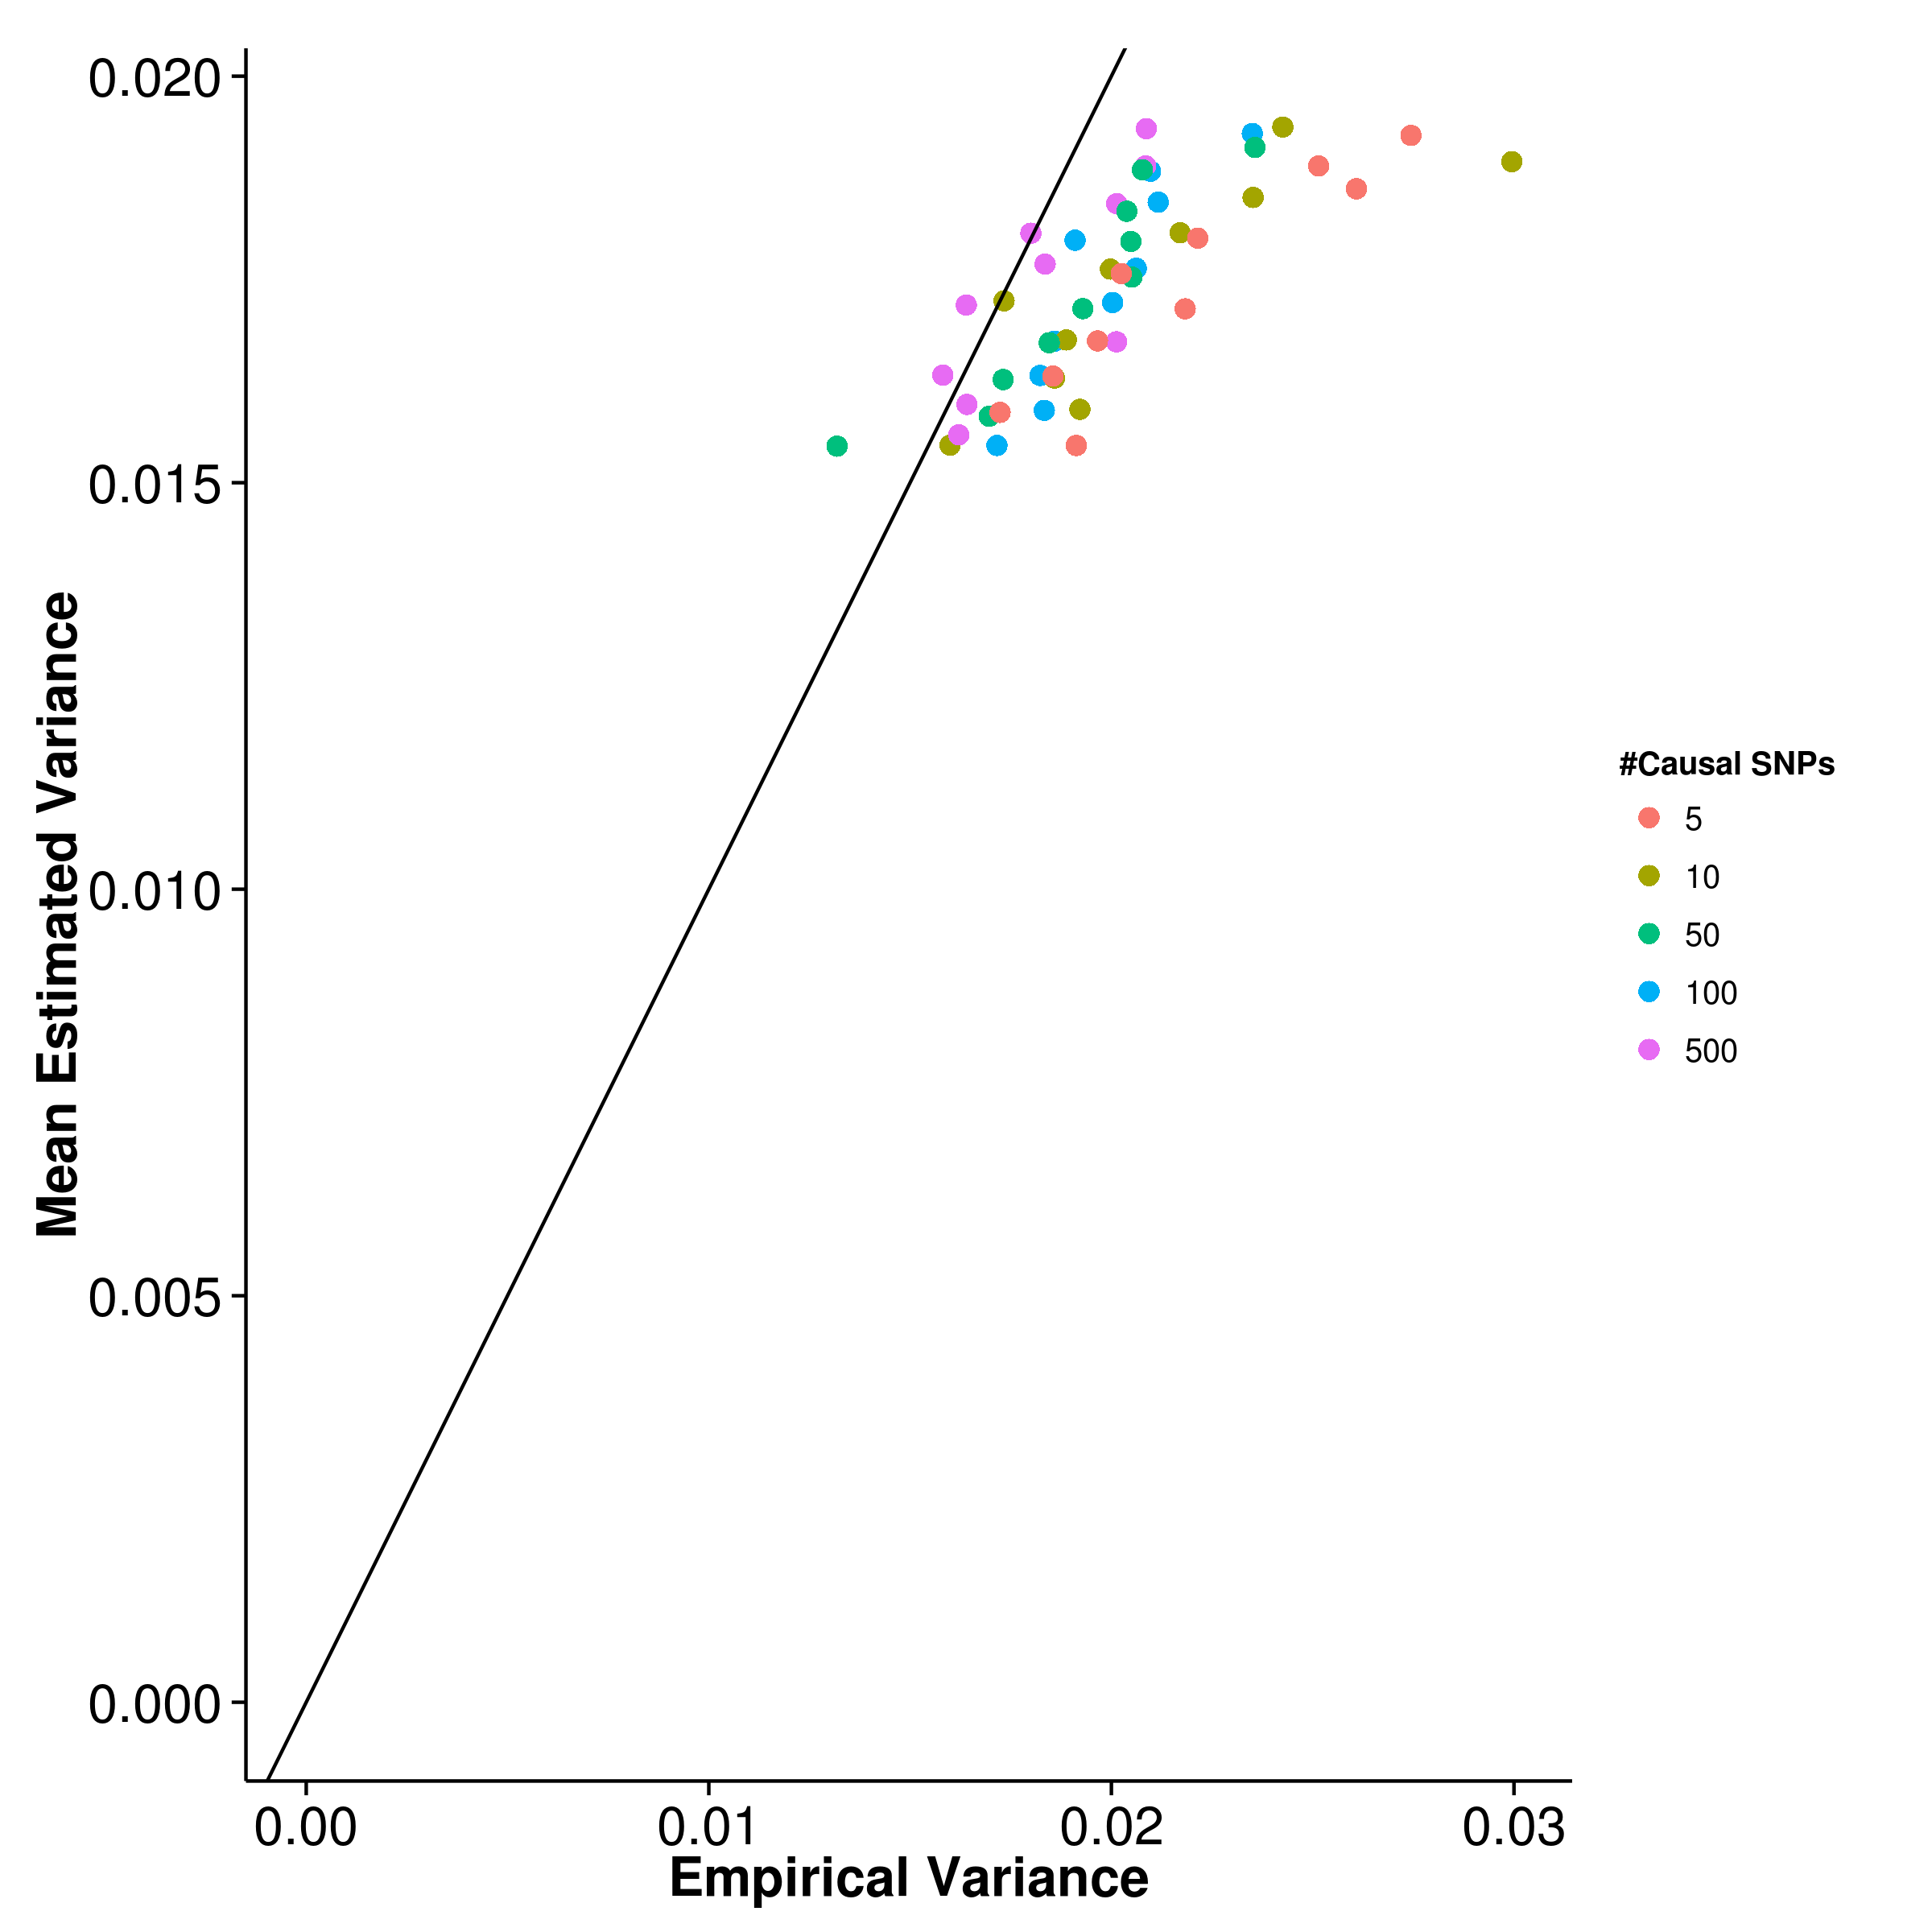
\includegraphics{figure/he_summary/random/shrek_Qt_Rand_sdCom.png}}
				\label{fig:shrekQtRandVarCom}
			}
			\subfloat[GCTA]{
				\scalebox{.4}{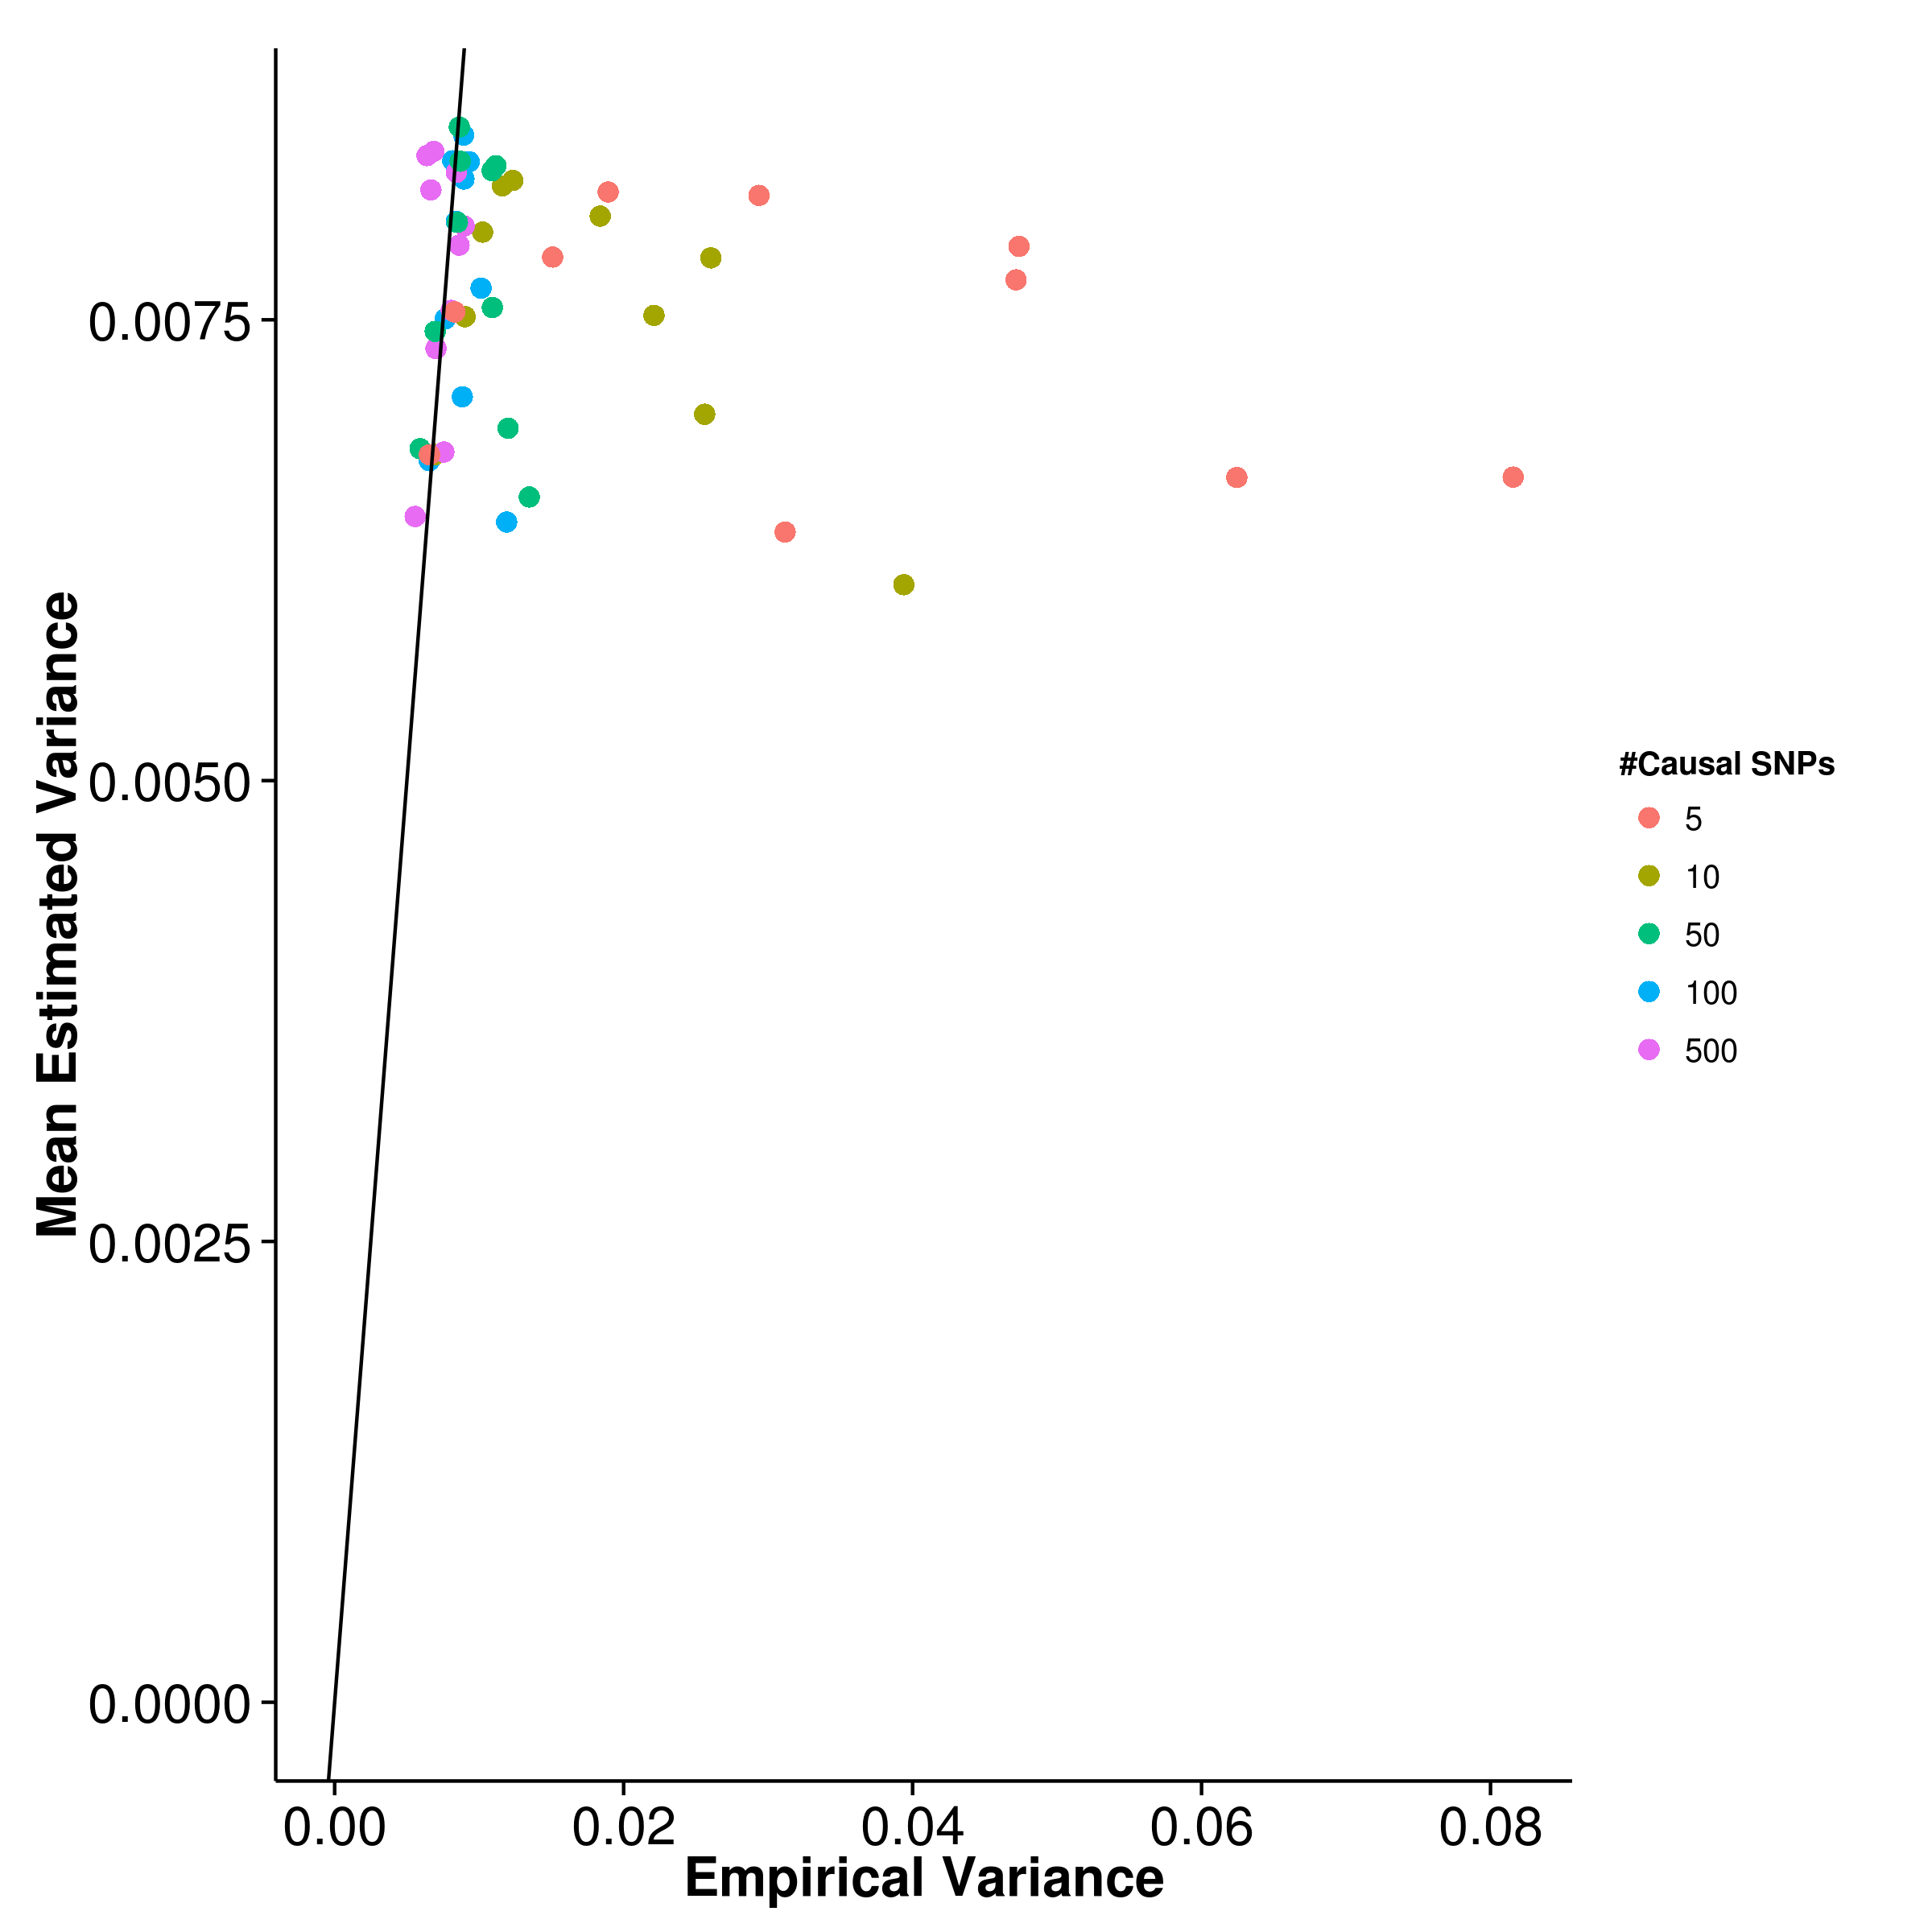
\includegraphics{figure/he_summary/random/gcta_Qt_Rand_sdCom.png}}
				\label{fig:gctaQtRandVarCom}
			}\\
			\subfloat[LDSC with fix intercept]{
				\scalebox{.4}{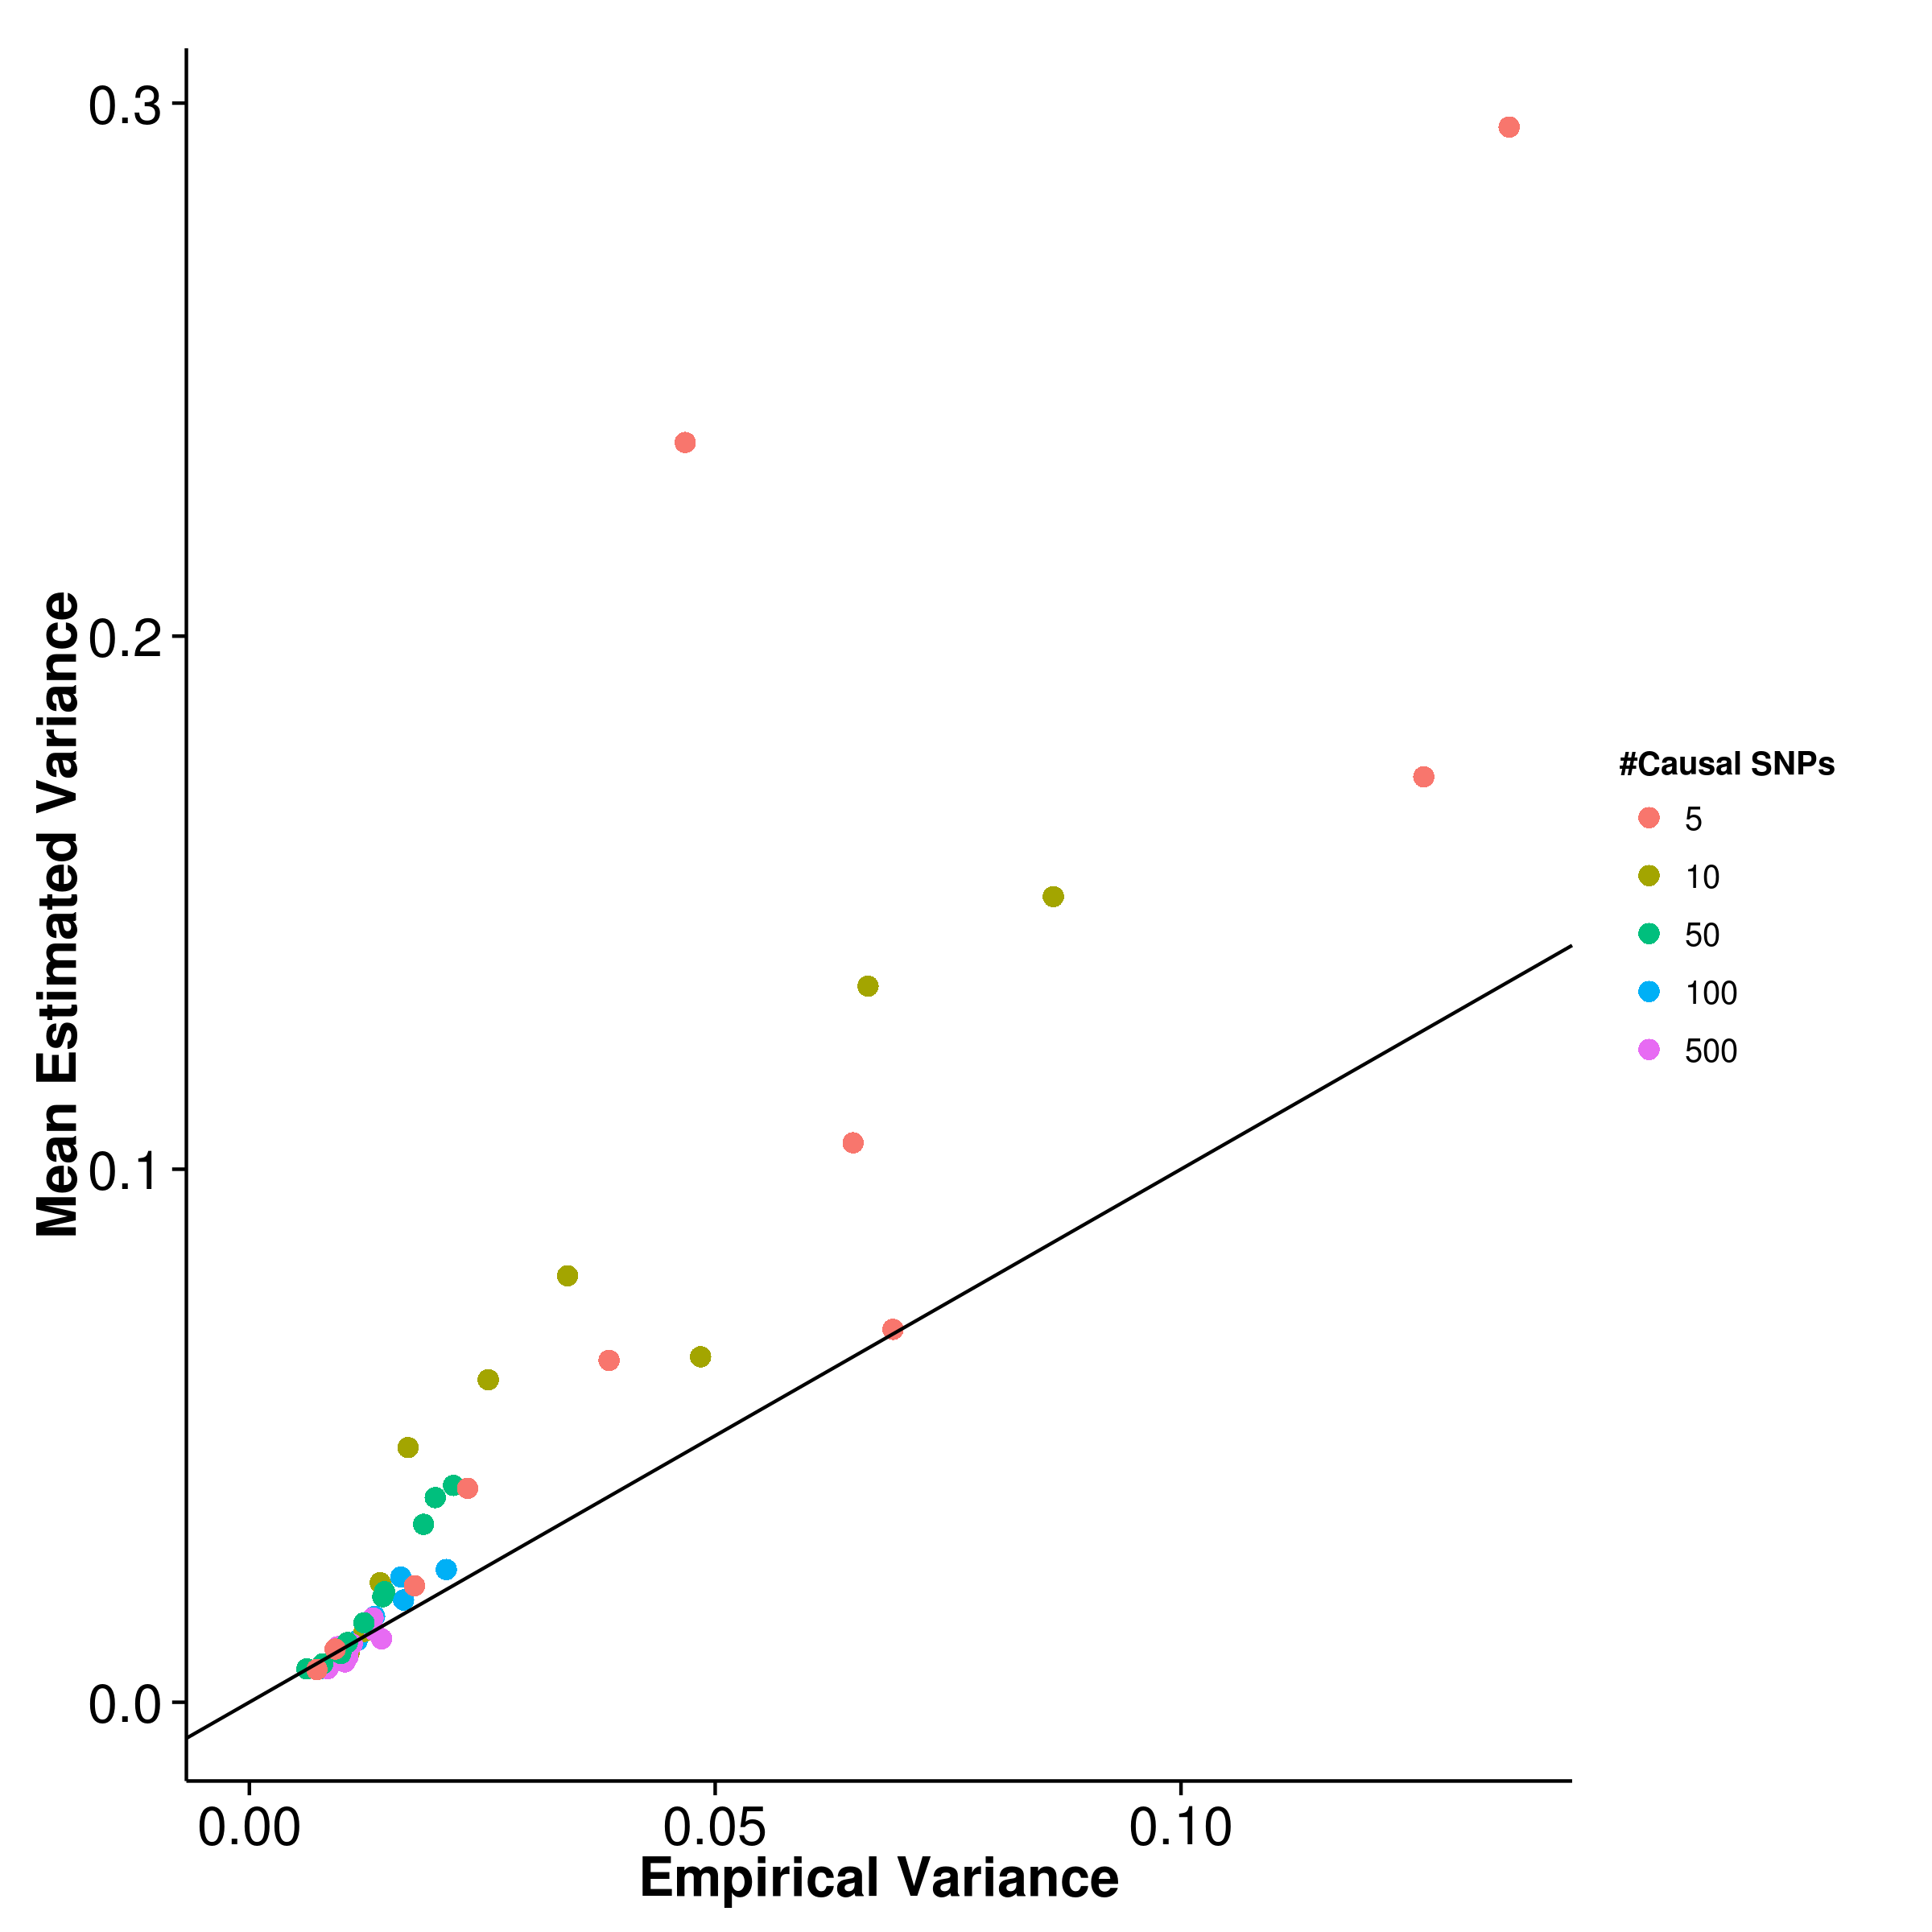
\includegraphics{figure/he_summary/random/ldsc_Qt_Rand_sdCom.png}}
				\label{fig:ldscQtRandVarCom}
			}
			\subfloat[LDSC with intercept estimation]{
				
				\scalebox{.4}{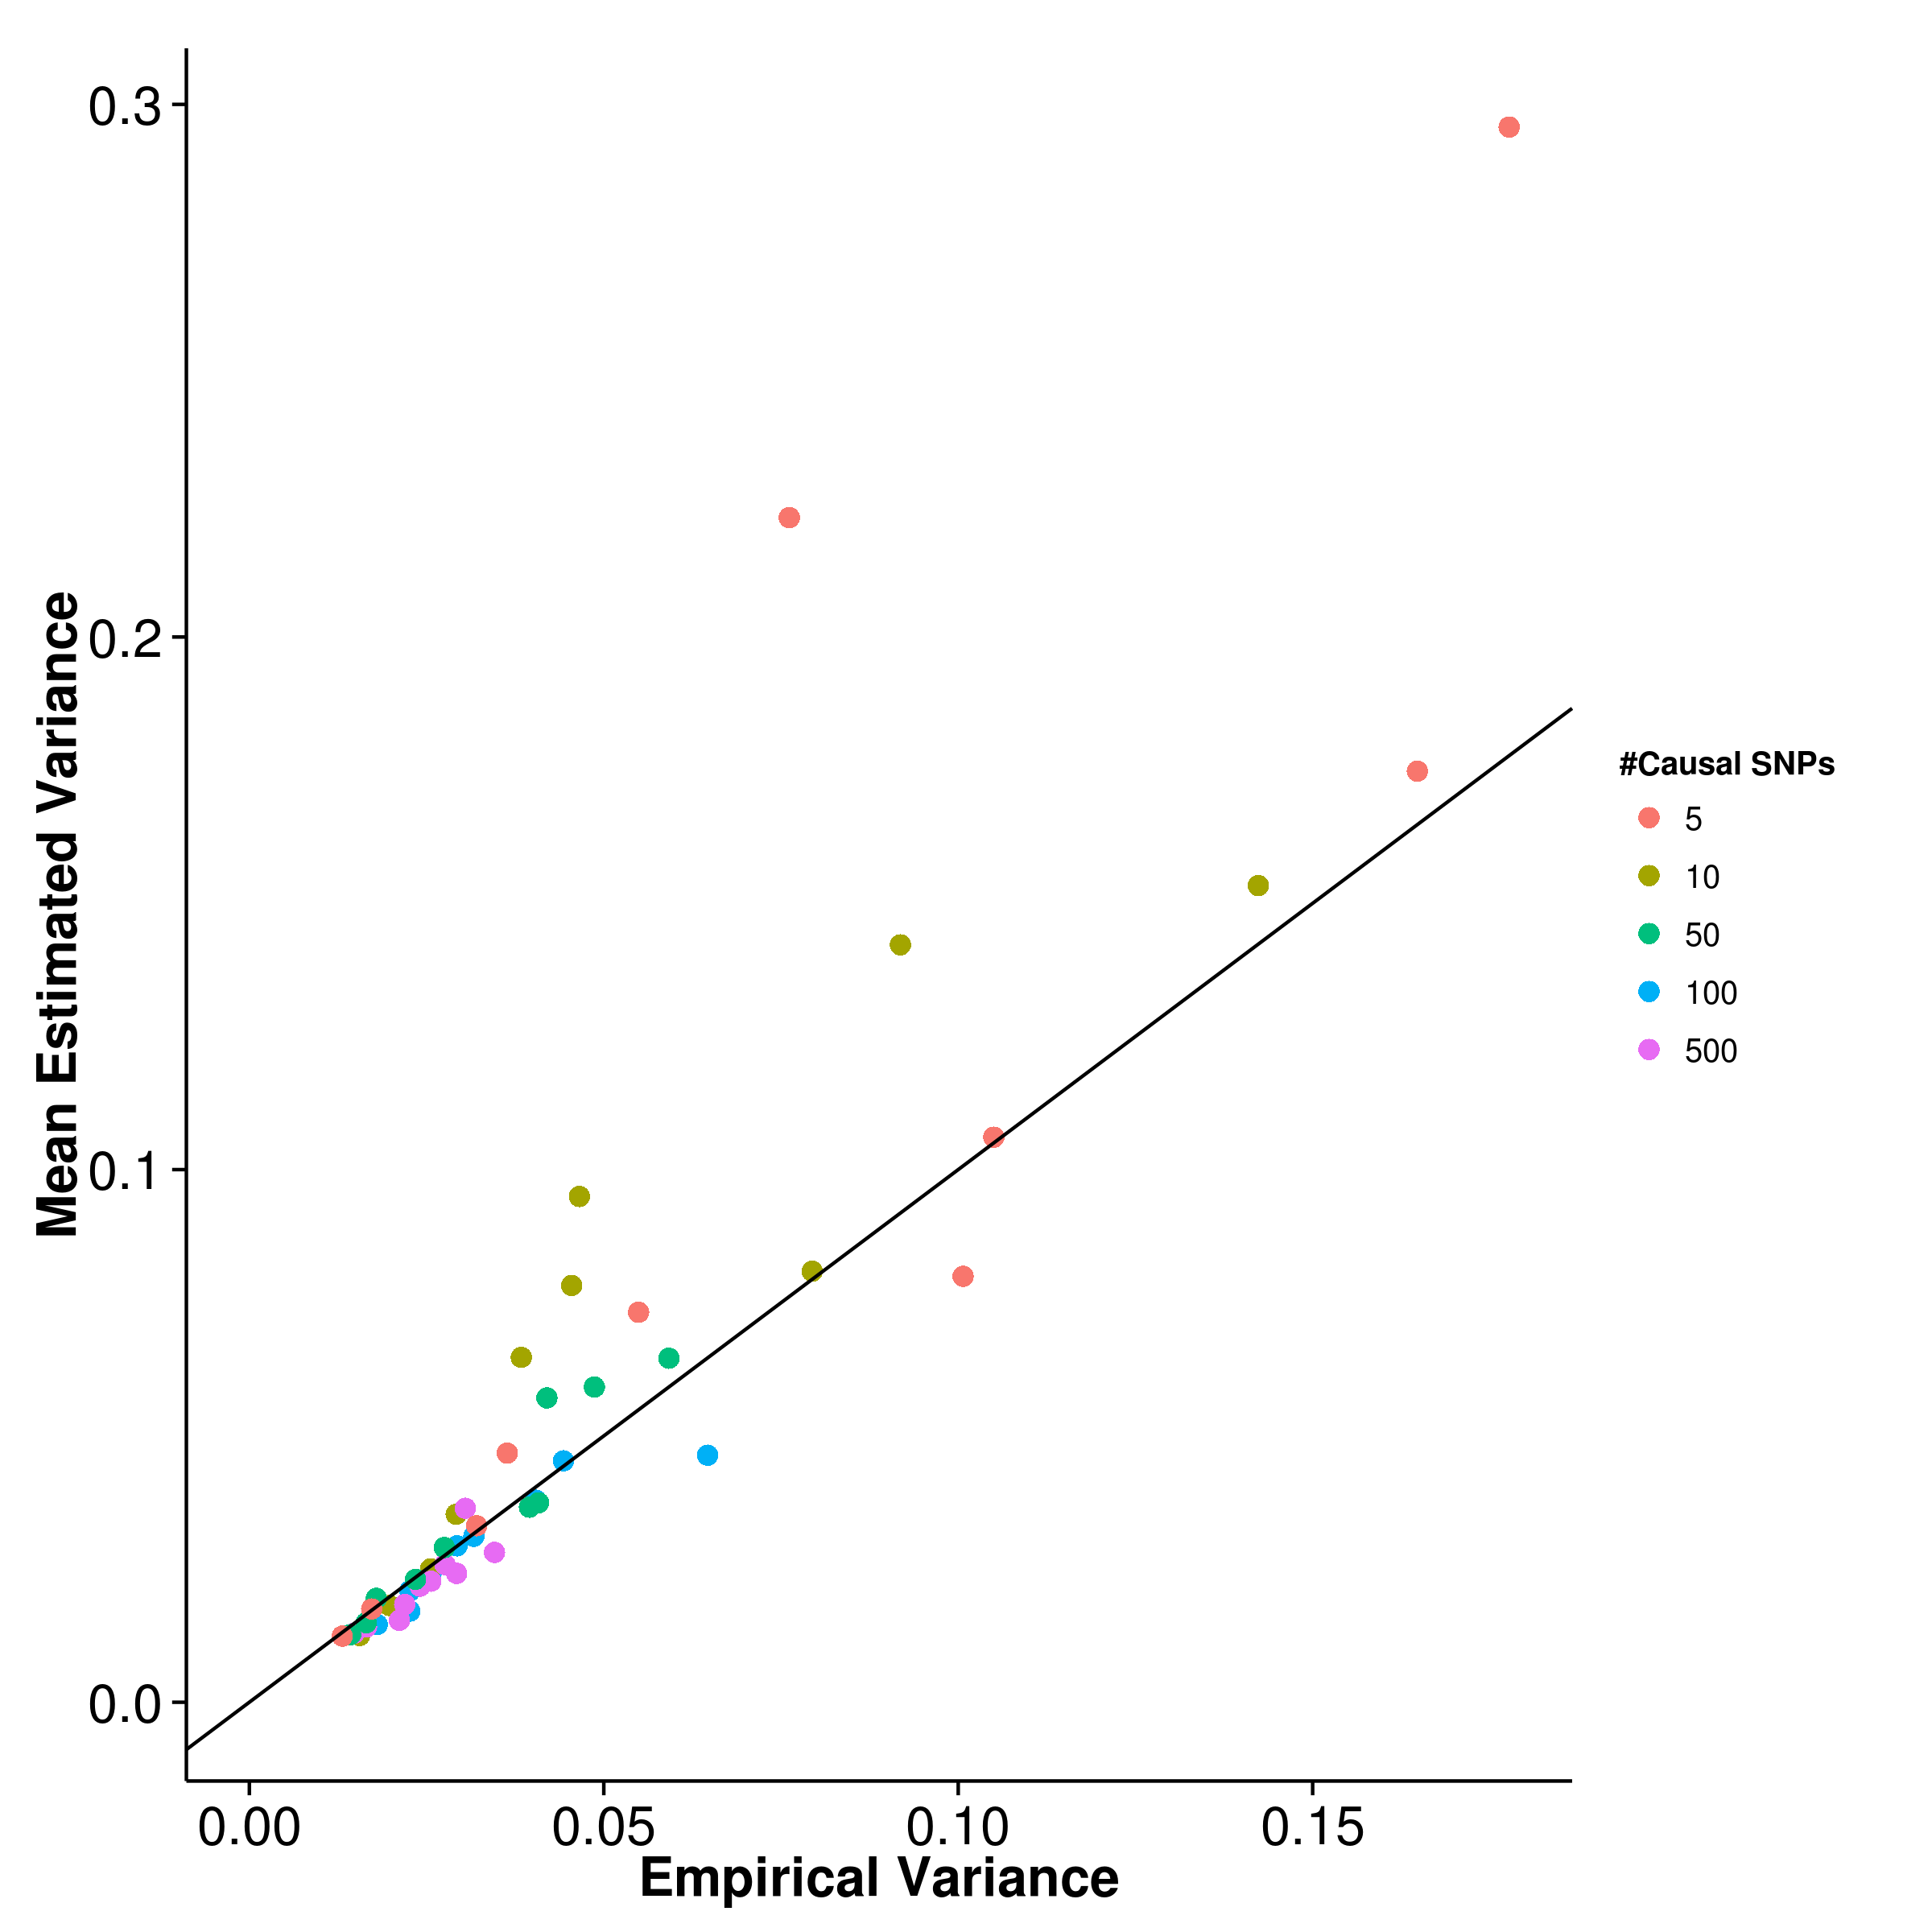
\includegraphics{figure/he_summary/random/ldscIn_Qt_Rand_sdCom.png}}
				\label{fig:ldscInQtRandVarCom}
			}
			\caption[Estimation of Variance in Quantitative Trait Simulation]
			{Estimated variance of results from quantitative trait simulation with random effect size simulation when compared to the empirical variance.
			\gls{gcta} has the best estimate of its empirical variance under the polygenic conditions whereas \gls{shrek} tends to under-estimate its empirical variance.
			On the other hand, \gls{ldsc} to over-estimate the variance especially when the number of causal \glspl{SNP} is small.
				} 
			\label{fig:QtRandVarCom}
		\end{figure}
		In the simulation of quantitative trait scenario, the effect size were randomly drawn from the exponential distribution with $\lambda=1$ and traits with different number of causal \glspl{SNP} and different narrow sense heritability were simulated.
		The main aim of this simulation was to assess the effect of number of causal \glspl{SNP} and trait heritability on the power of estimation of different algorithms.
		
		First, the mean heritability estimation were compared to the simulated heritability in order to identify the bias in estimation for each algorithms.
		From the graph (\cref{fig:QtRandMean}), it was observed that the mean estimations of \gls{shrek} were very close to the simulated heritability (\cref{fig:shrekQtRandMean}), with a slight downward bias. 
		Moreover, the bias was insensitive to the change in number of causal \glspl{SNP} suggesting that \gls{shrek} might be relatively robust to trait complexity.
		Similarly, estimations form \gls{gcta} were also accurate and were only moderately biased upward (\cref{fig:gctaQtRandMean}). 
		On the other hand, the bias observed in the estimations from \gls{ldsc} were relatively large when compared to \gls{shrek} and \gls{gcta}.
		No matter if the intercept was estimated or fixed, estimations from \gls{ldsc} were upwardly biased and increases as the trait heritability increases (\cref{fig:ldscQtRandMean,fig:ldscInQtRandMean}).
		The only exception was when there were only 5 causal \glspl{SNP} in which a large downward bias was detected when the intercept estimations function was used. 
		
		Furthermore, while comparing the empirical variance of the estimates (\cref{fig:QtRandVar}), variance of estimations from \gls{ldsc} were sensitive to the number of causal \glspl{SNP} where as the number of causal \glspl{SNP} decreases (\cref{fig:ldscQtRandVar,fig:ldscInQtRandVar}), the variance increases, similar to what was reported by \citet{Bulik-Sullivan2015}.
		The variance were also higher when intercept estimation was performed. 
		On the other hand, although the variance of \gls{shrek} was relatively higher when compared to \gls{ldsc} when the intercept was fixed, the variation of its estimations was insensitive to the number of causal \glspl{SNP}, when the number of causal \glspl{SNP} was small, the variance of estimation from \gls{shrek} can be even be lower than \gls{ldsc} (\cref{fig:shrekQtRandVar}).
		Finally, of all the algorithms, the estimations from \gls{gcta} has the lowest variation when compared to other algorithm (\cref{fig:gctaQtRandVar}), except when it was the case of 5 causal \glspl{SNP} where it has a slightly higher variance when compared to \gls{shrek} when the simulated heritability was high (e.g. $\ge 0.8$).
		
		%TODO Variance Variance Graph need to redrawn such that at least all the abline were 45'
		Another important factor to consider was the estimation of the \gls{se}. 
		Of all the algorithms, \gls{gcta} (\cref{fig:gctaQtRandVarCom}) has the best estimate, follow by \gls{shrek} (\cref{fig:shrekQtRandVarCom}).
		However, it was noted that \gls{shrek} tends to under-estimate the variance ($\sim0.9$ fold) and its estimates were slightly affected by the number of causal \glspl{SNP}.
		On the other hand, \gls{ldsc} cannot accurately estimate its variance especially when the number of causal \glspl{SNP} were small. 
		When intercept estimations was performed (\cref{fig:ldscInQtRandVarCom}), the estimation of variance was relatively better ($\sim1.25$ fold) when compared to the case where fixed intercept was used ($\sim1.65$ fold) instead (\cref{fig:ldscQtRandVarCom}). 
		
		Overall, by taking into consideration of both the bias and variance of the estimates, \gls{gcta} has the best performance, follow by \gls{shrek}. 
		The \gls{ldsc} with fixed intercept performs better than \gls{ldsc} with intercept estimation except in the case of variance estimation. 
		An interesting property of \gls{shrek} is that it is insensitive to number of causal \gls{SNP} of the trait, making it idea for the estimation of narrow sense heritability when one is uncertain of the genetic architecture of the trait and when the sample genotypes are unavailable.
		\begin{table}
			\centering
			\begin{tabular}{rrrrr}
				\toprule
				Number of Causal SNPs&	SHREK&	LDSC&	LDSC-In&	GCTA \\
				\midrule
				5	&	0.177	&	0.565	&	0.584	&	0.230\\
				10	&	0.159	&	0.251	&	0.470	&	0.151\\
				50	&	0.153	&	0.179	&	0.378	&	0.0796\\
				100	&	0.157	&	0.166	&	0.305	&	0.0794\\
				250	&	0.152	&	0.144	&	0.266	&	0.0674\\
				500	&	0.143	&	0.134	&	0.247	&	0.0646\\
				\bottomrule
			\end{tabular}
			\caption[Mean Squared Error of Quantitative Trait Simulation with Random Effect Size]{
				\gls{mse} of quantitative trait simulation with random effect size.
				Of all the algorithms, \gls{gcta} has the lowest \gls{mse} except when there is only 5 causal \glspl{SNP} and the performance of \gls{shrek} and \gls{ldsc} with fix intercept converges as number of causal \glspl{SNP} increases. 
				\gls{ldsc} with fix intercept even surpassed \gls{shrek}'s performance when the number of causal \glspl{SNP} was as high as 500.}
			\label{tab:mseQtRandom}
		\end{table}
		% Extreme with 100 causal
		
		\subsection{Quantitative Trait Simulation with Extreme Effect Size}
		
		\begin{figure}
			\centering
			\subfloat[SHREK]{
				\scalebox{.4}{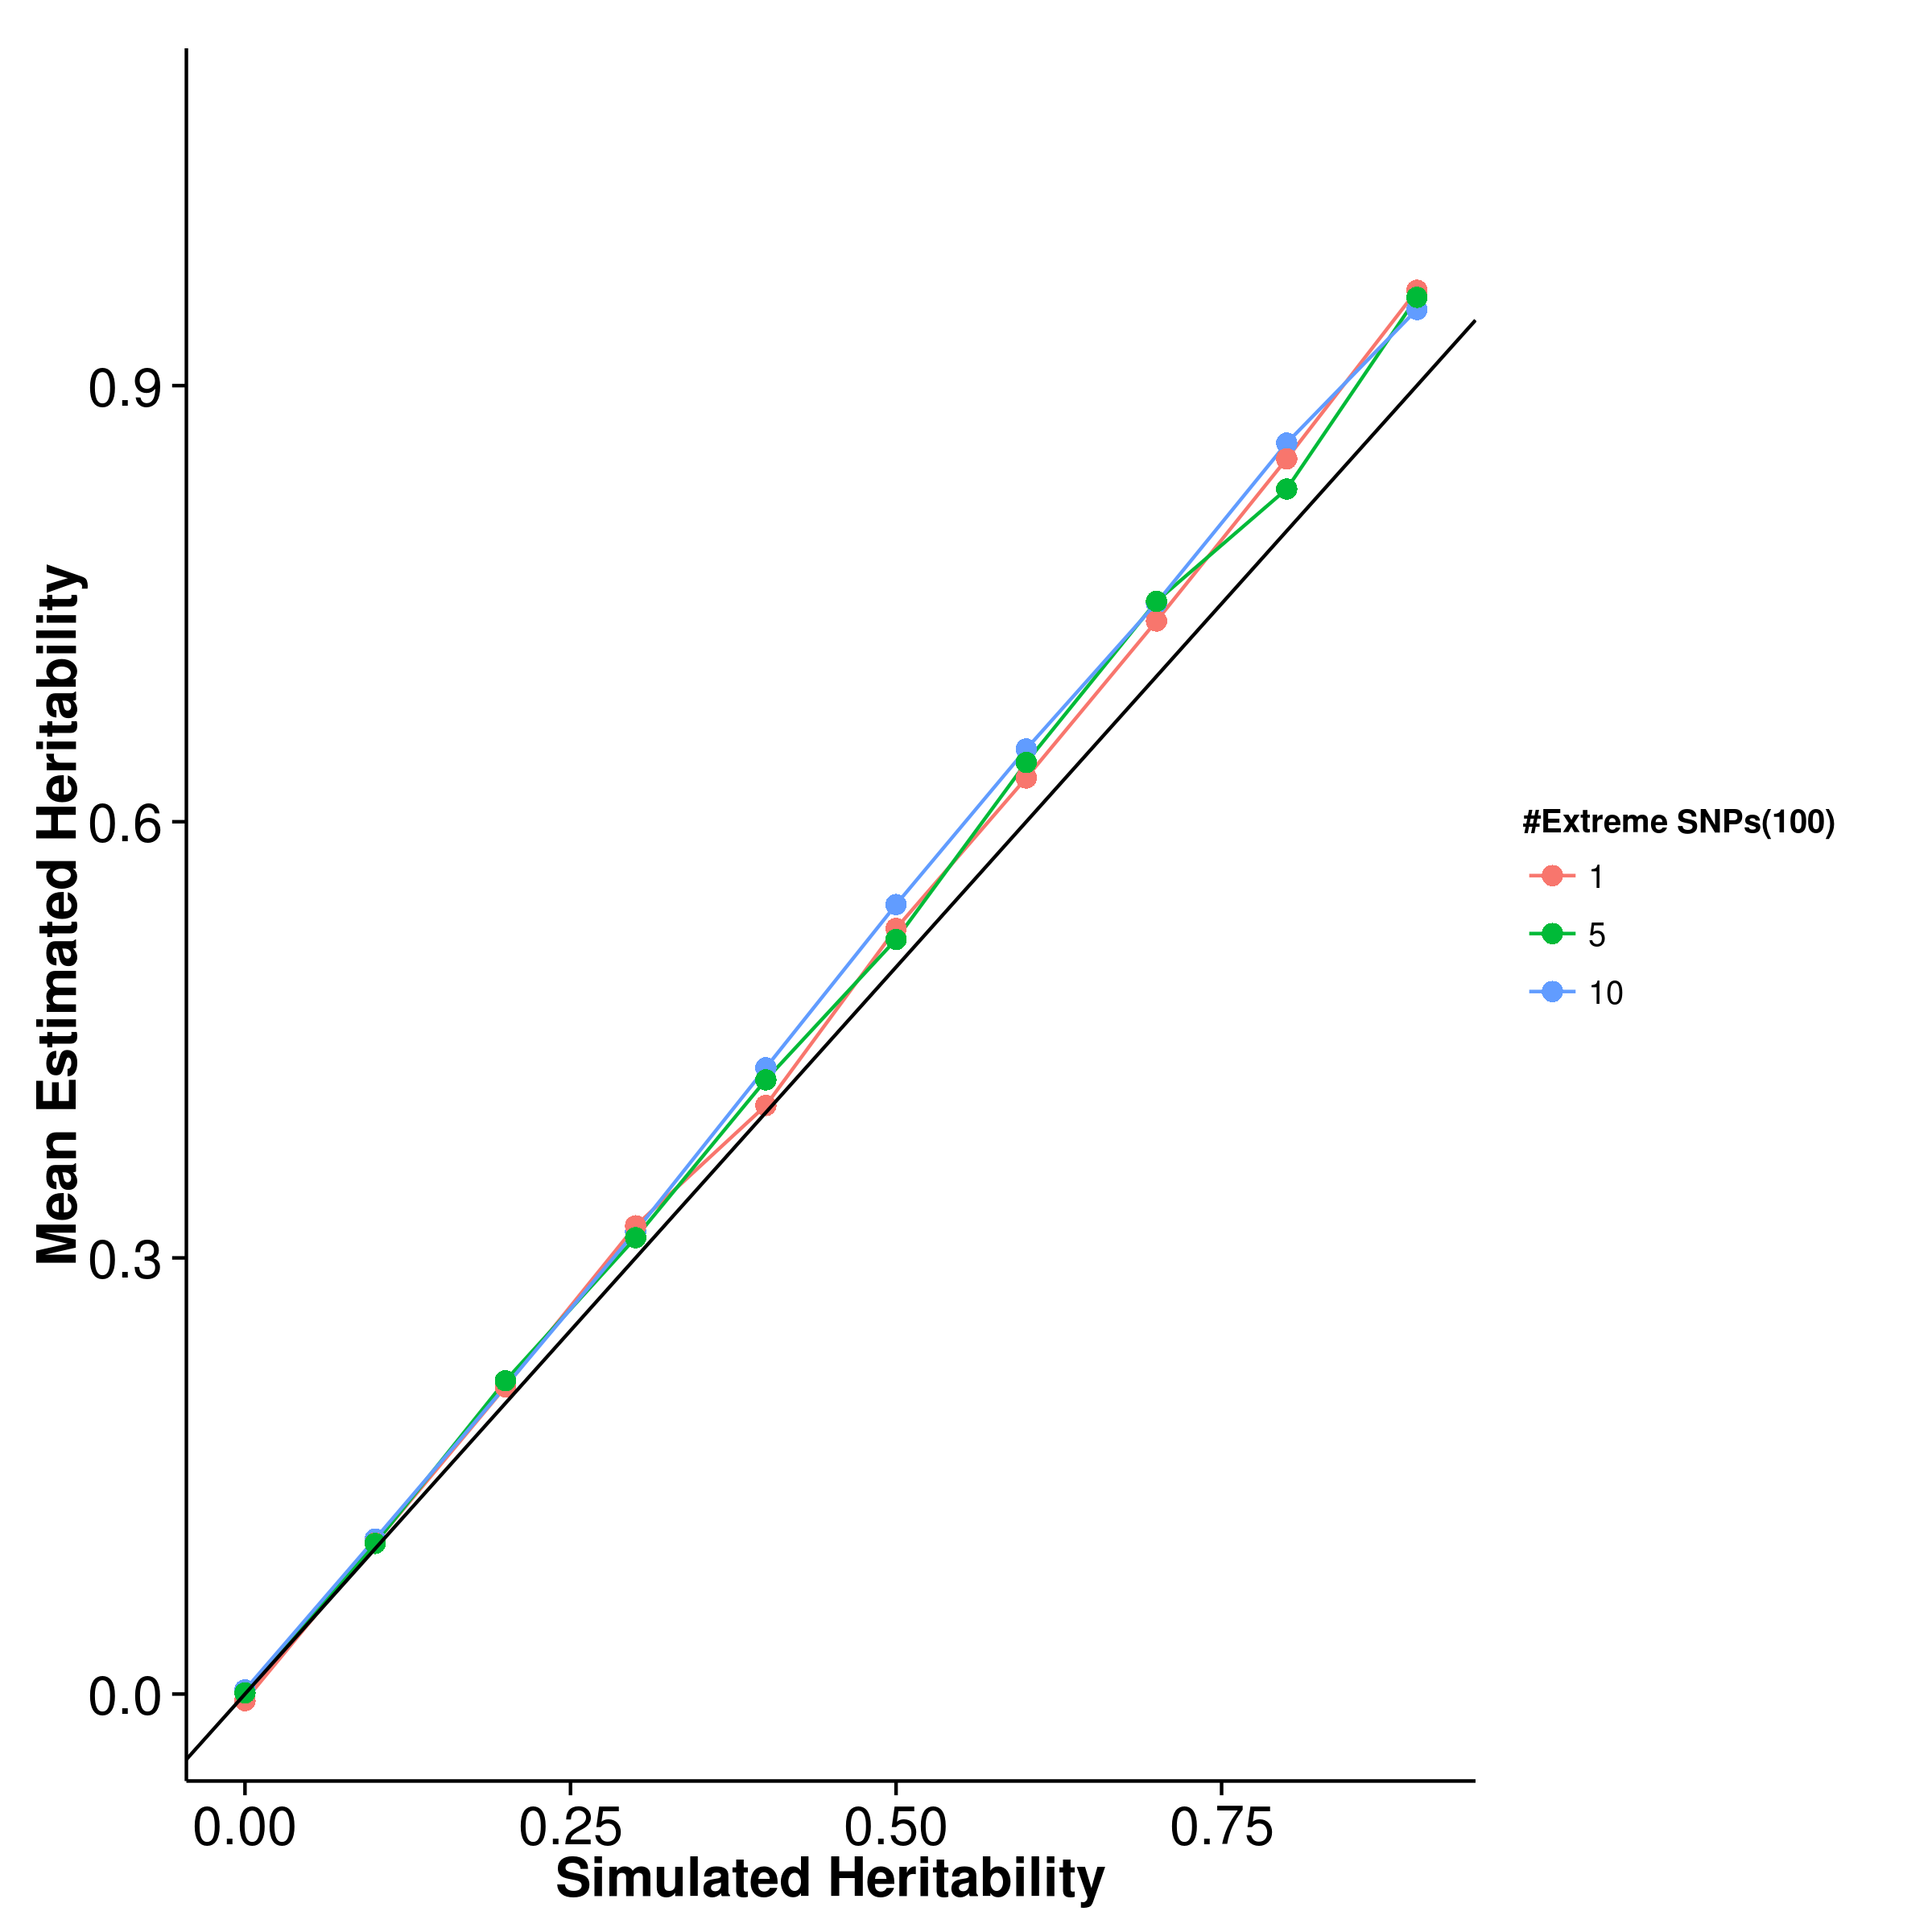
\includegraphics{figure/he_summary/extreme_100c/shrek_QtE_Rand_mean.png}}
				\label{fig:shrekQtEx100cMean}
			}
			\subfloat[GCTA]{
				\scalebox{.4}{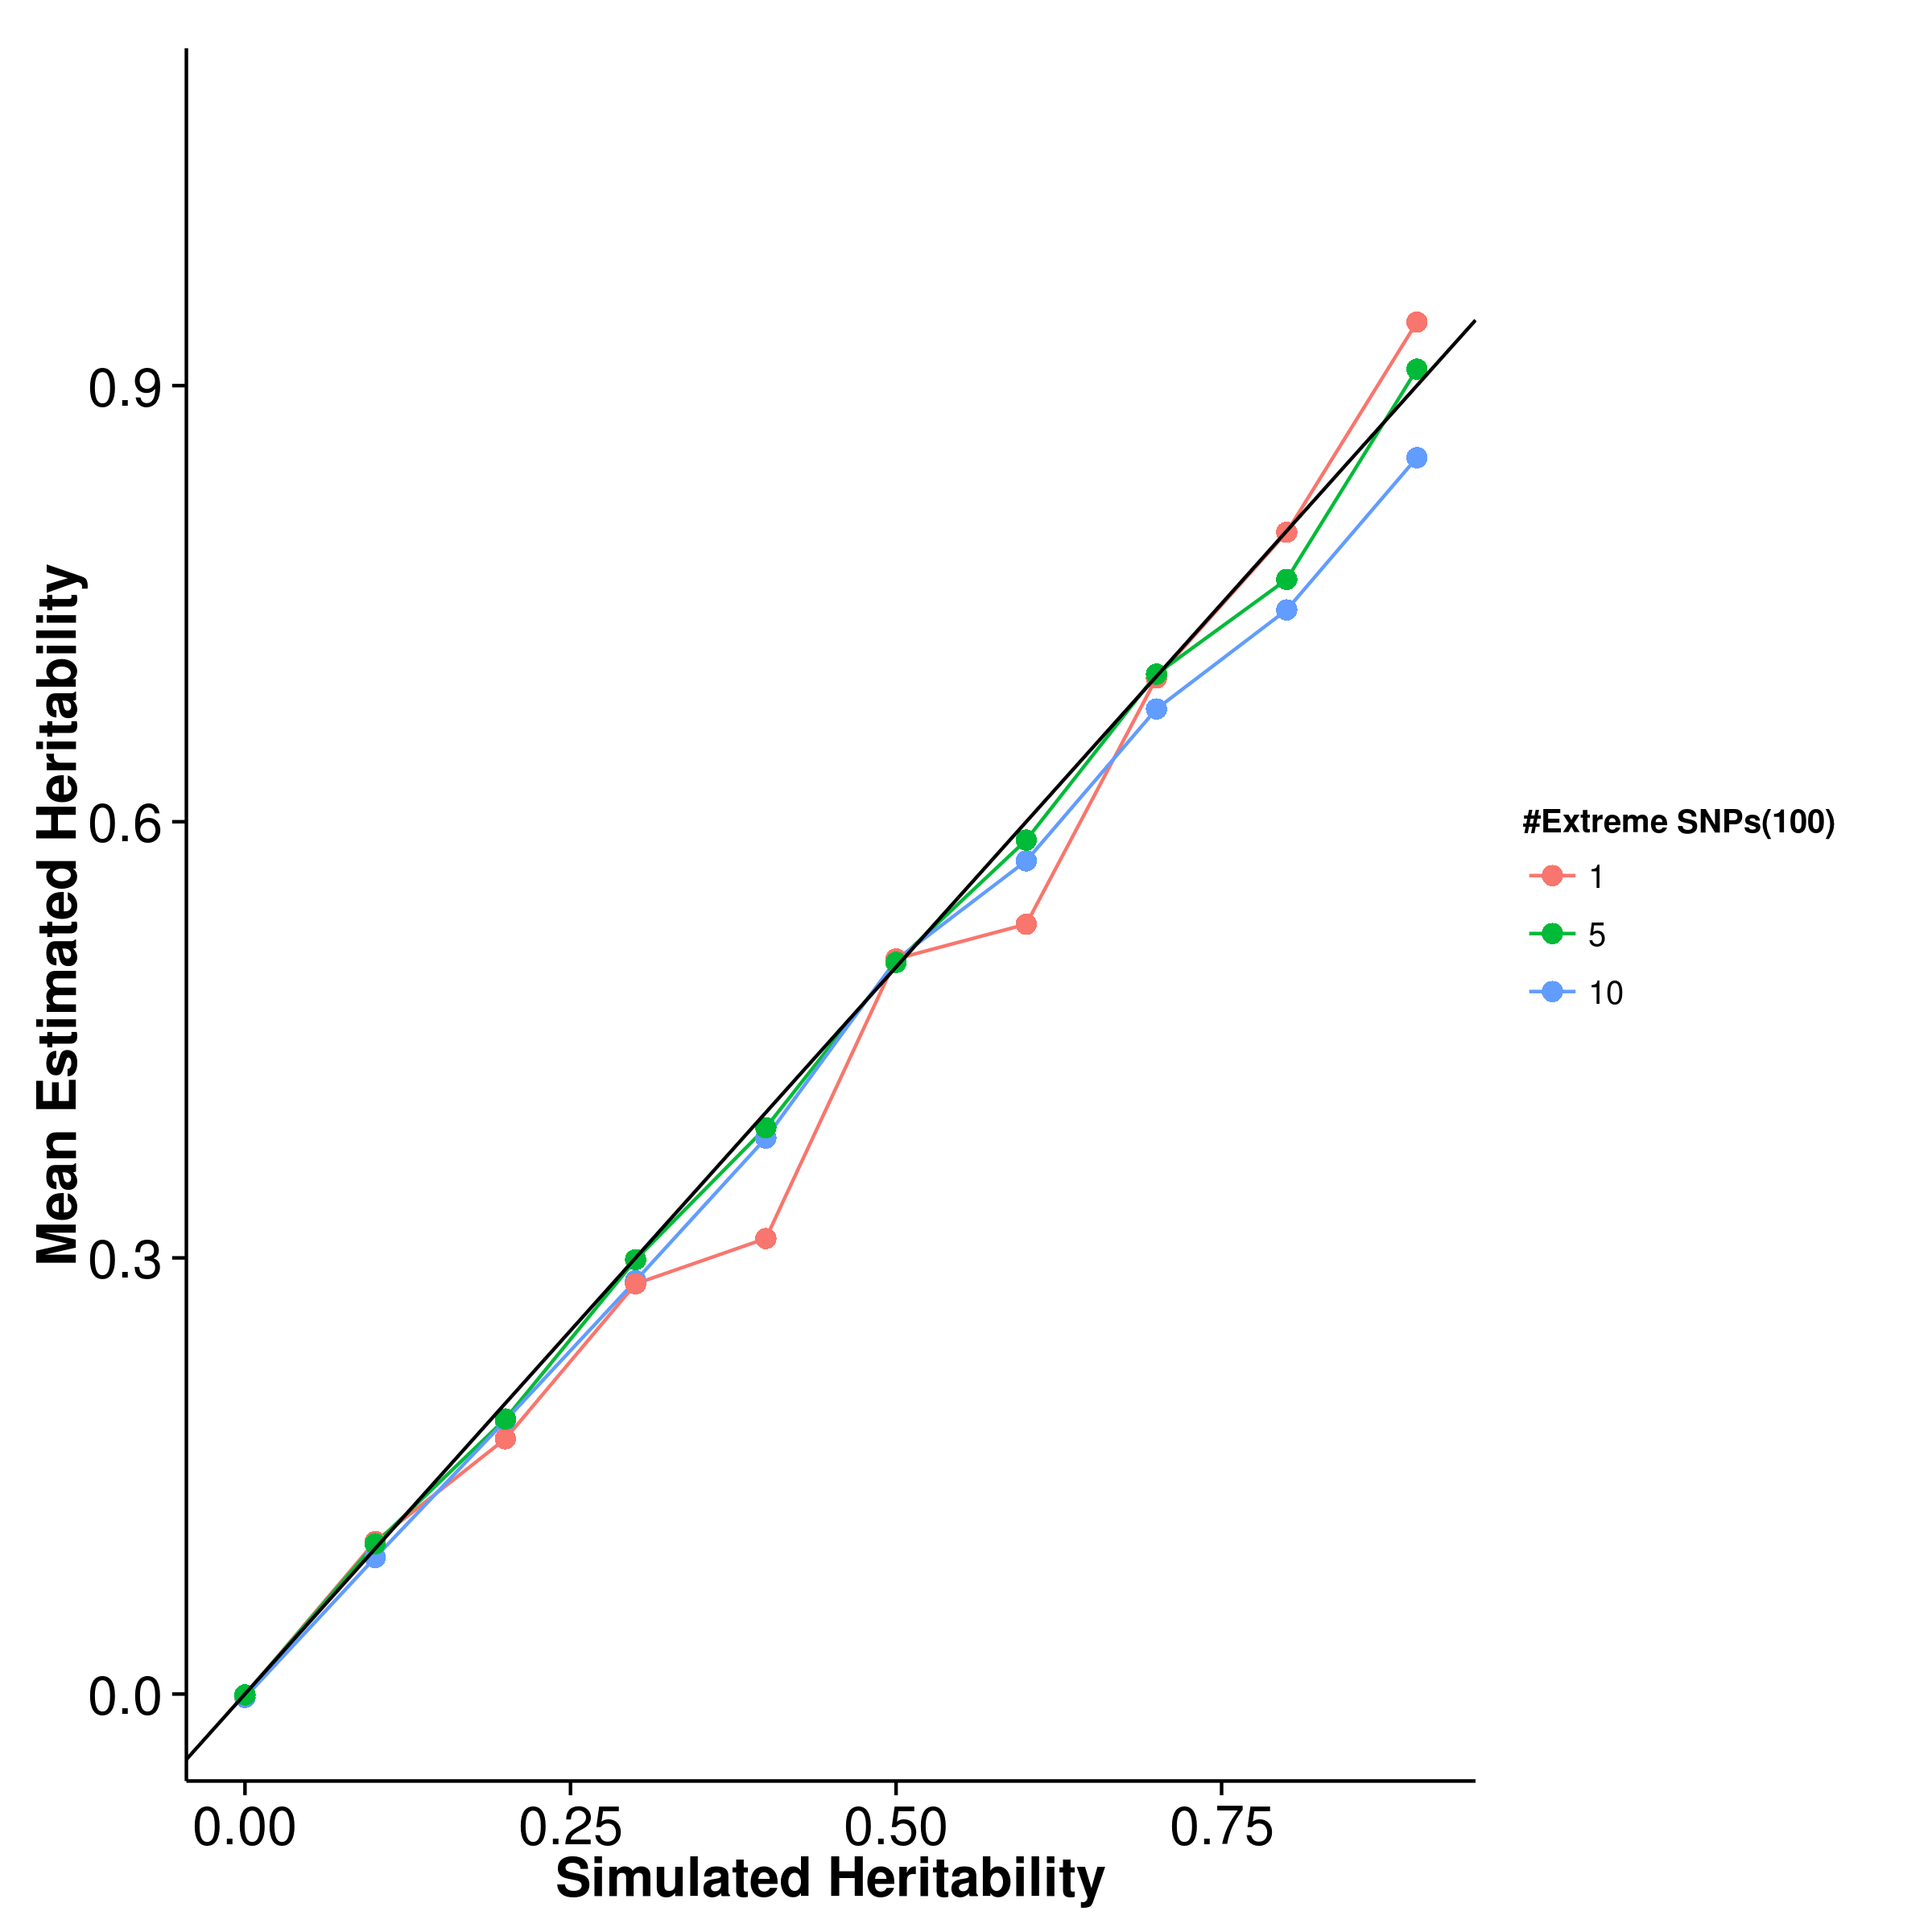
\includegraphics{figure/he_summary/extreme_100c/gcta_QtE_Rand_mean.png}}
				\label{fig:gctaQtEx100cMean}
			}\\
			\subfloat[LDSC with fix intercept]{
				\scalebox{.4}{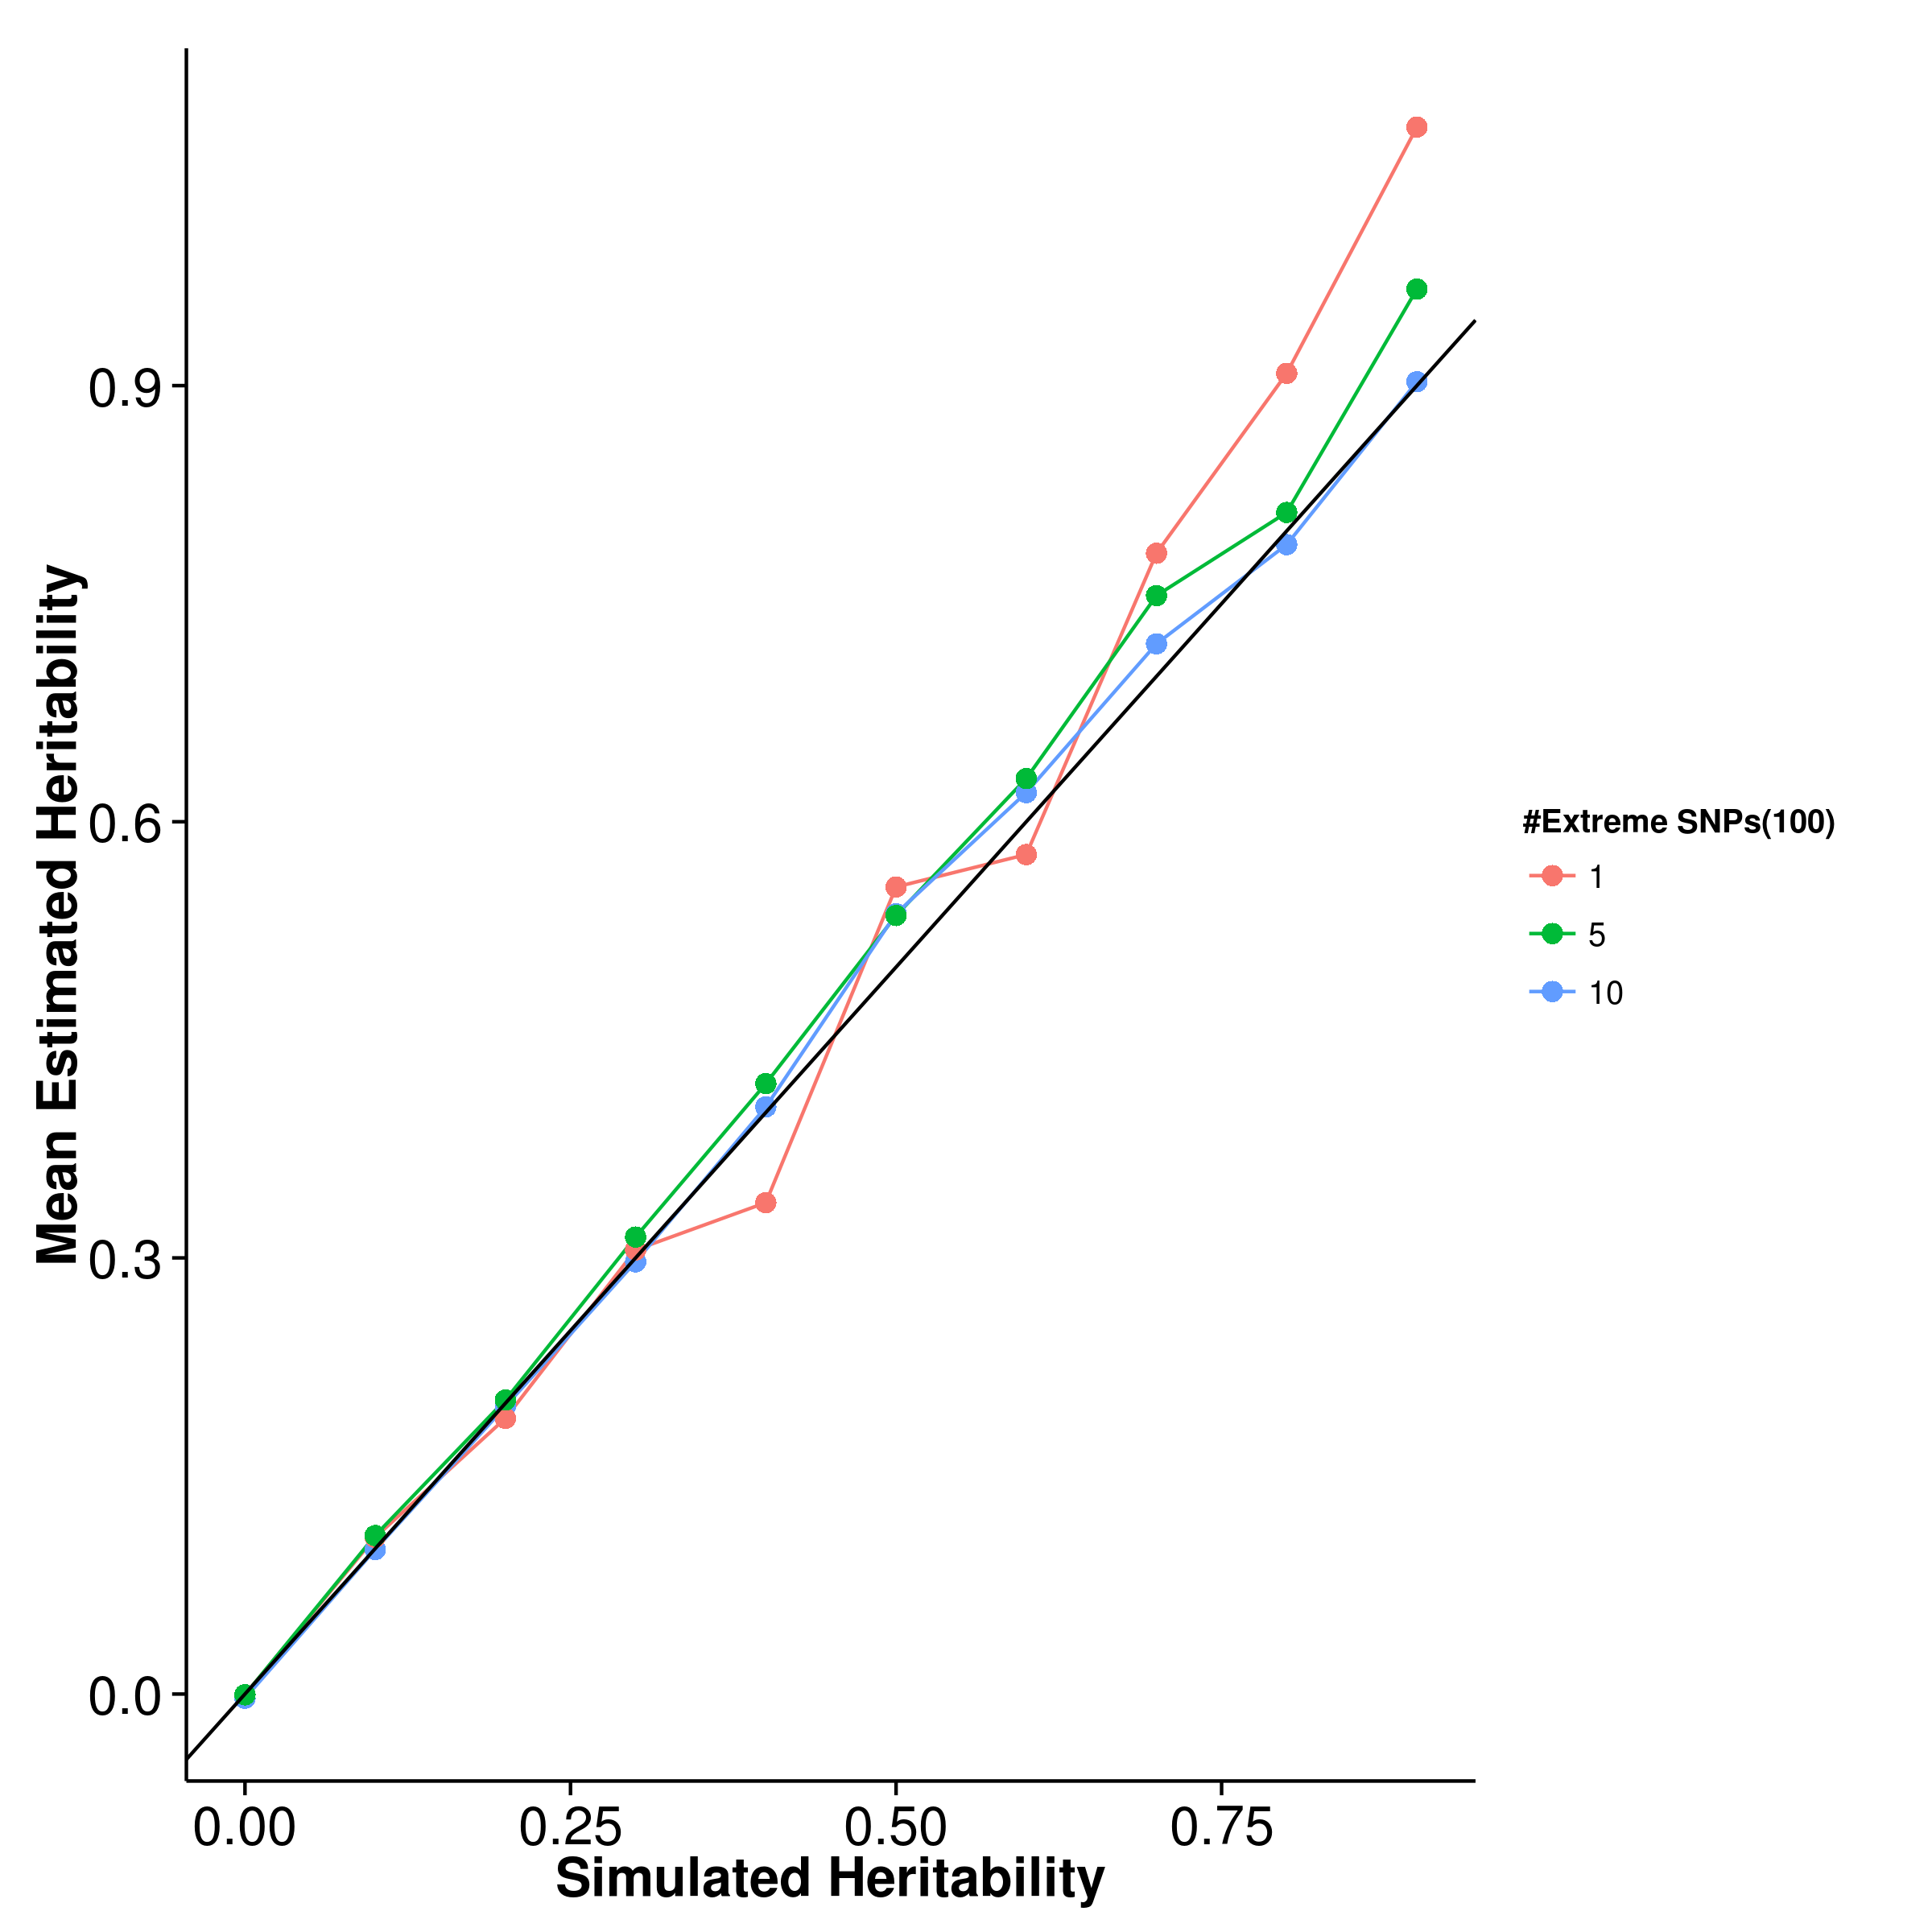
\includegraphics{figure/he_summary/extreme_100c/ldsc_QtE_Rand_mean.png}}
				\label{fig:ldscQtEx100cMean}
			}
			\subfloat[LDSC with intercept estimation]{
				
				\scalebox{.4}{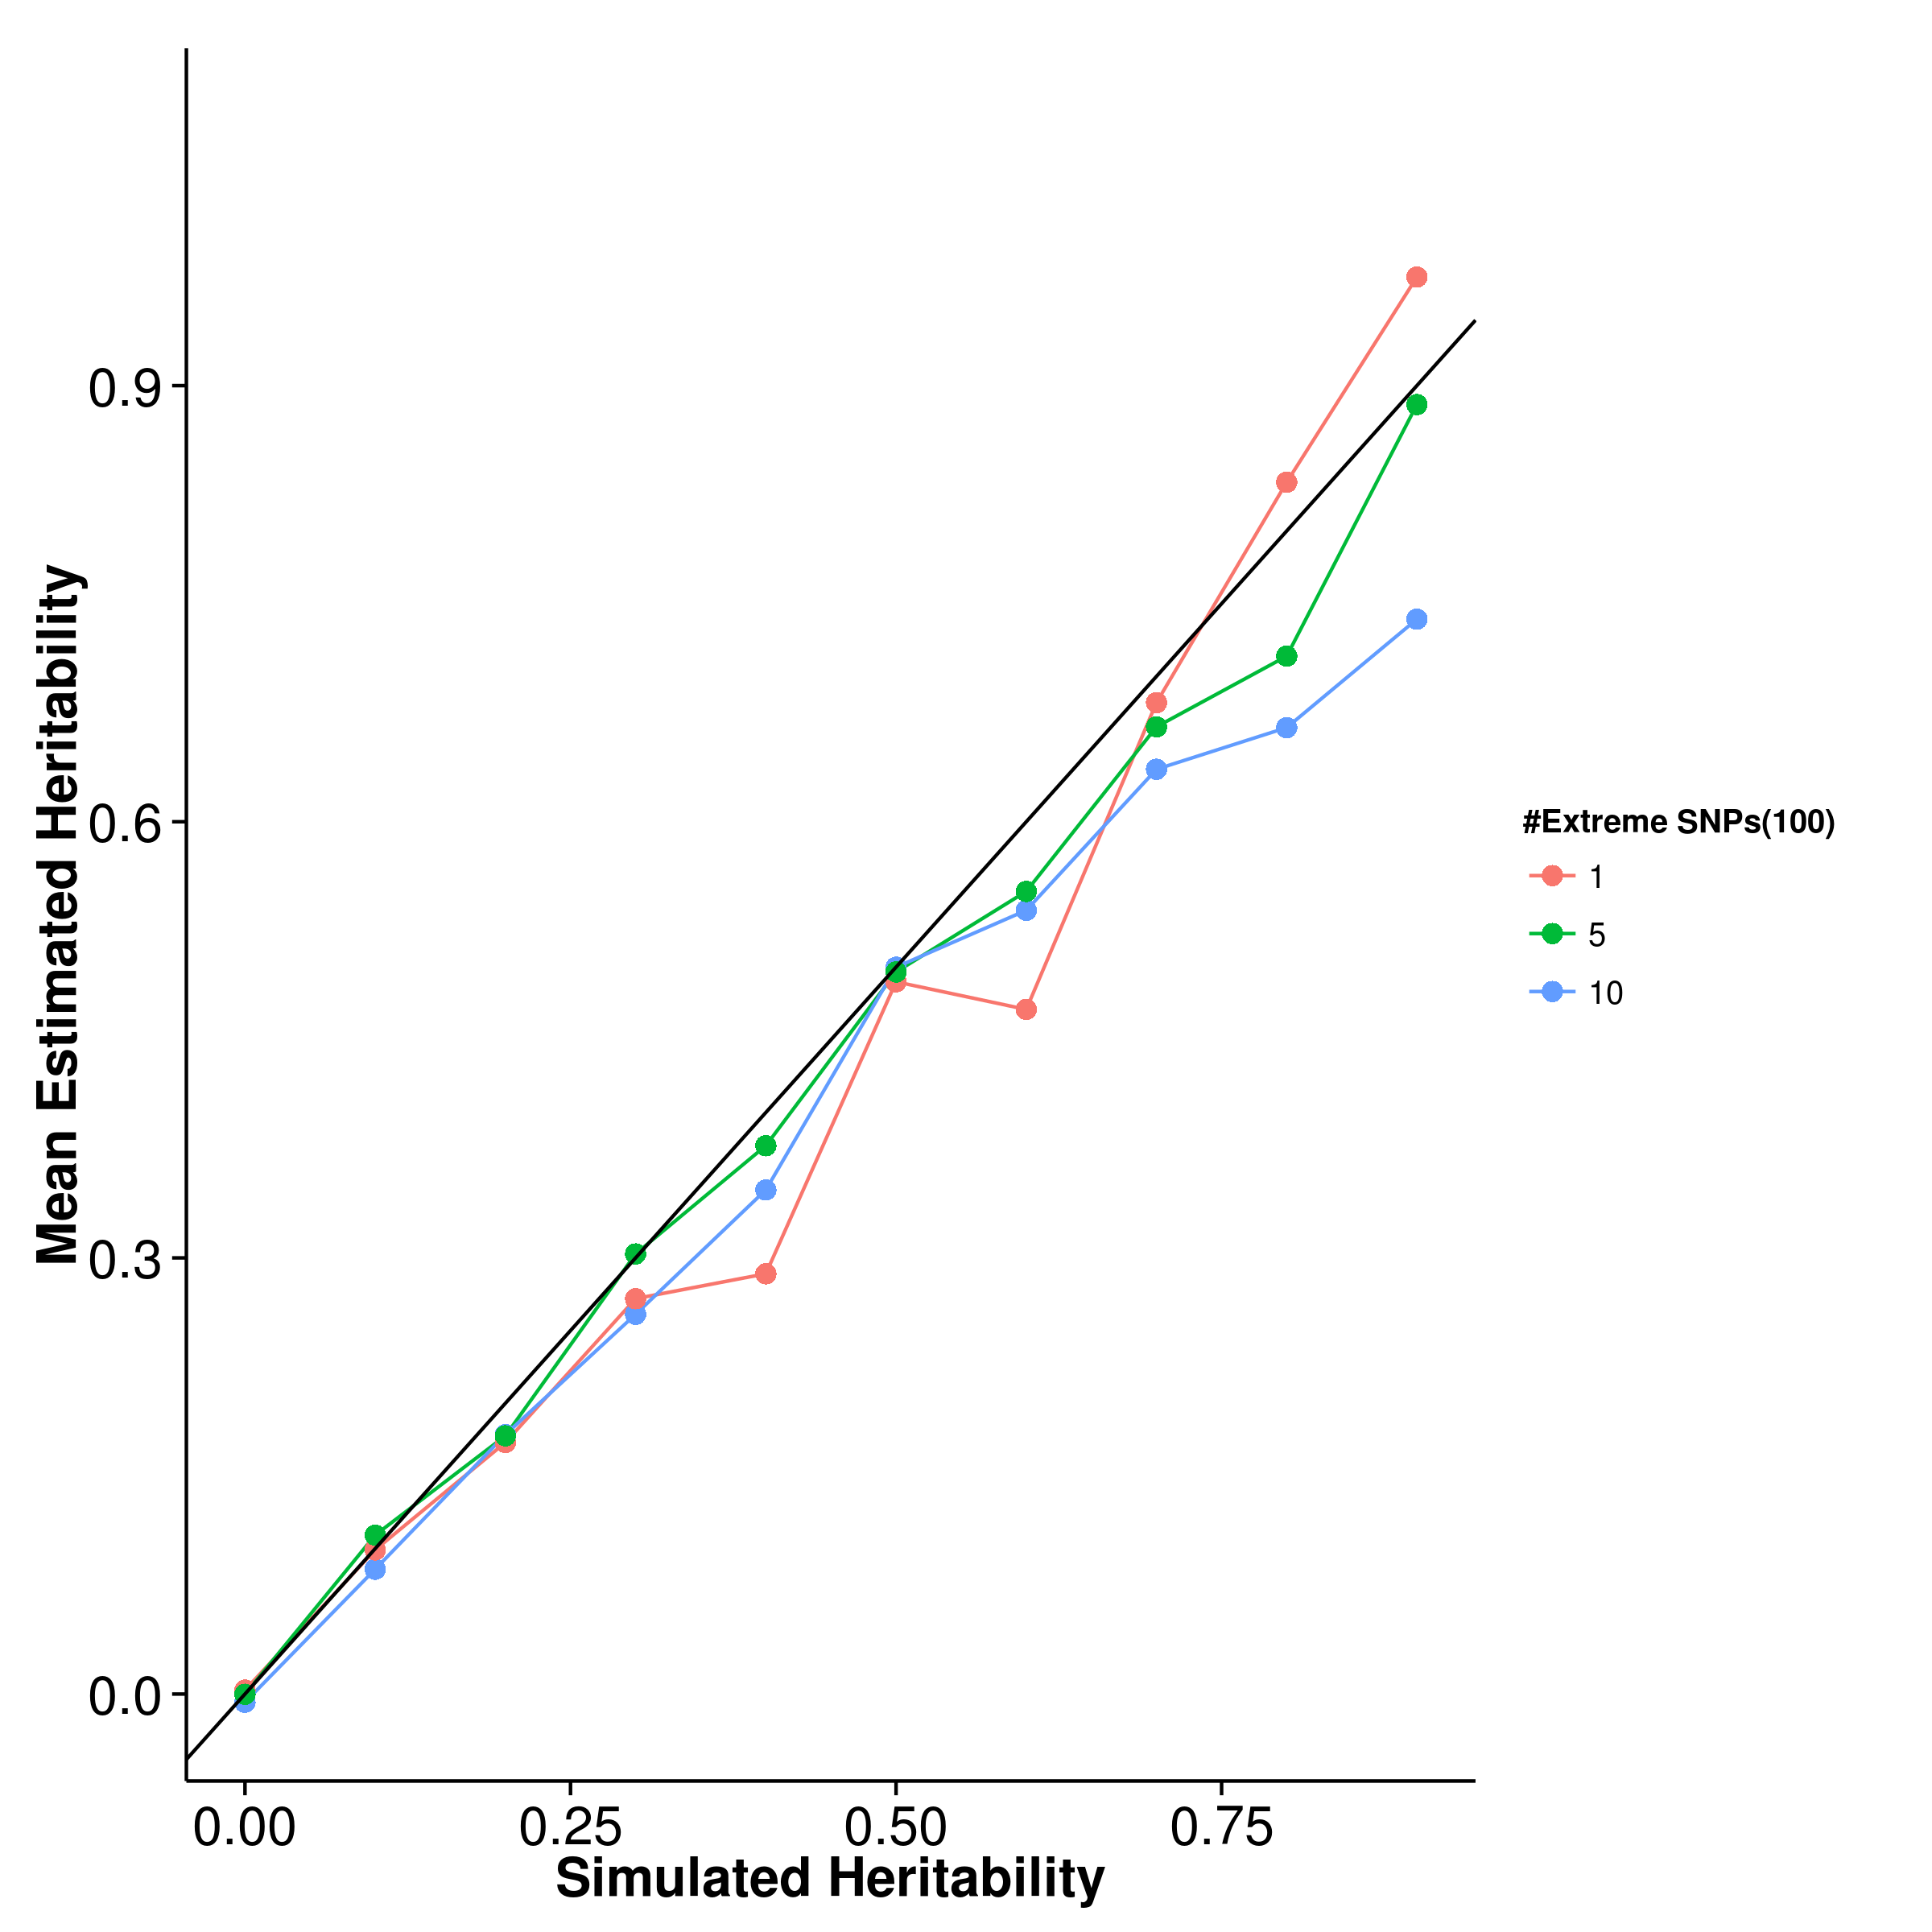
\includegraphics{figure/he_summary/extreme_100c/ldscIn_QtE_Rand_mean.png}}
				\label{fig:ldscInQtEx100cMean}
			}
			\caption[Mean of Extreme Effect Size Simulation Result]
			{Mean of results from quantitative trait simulation with extreme effect size simulation.
				It was observed that the mean estimation of heritability of \gls{shrek} is not affected by the number of \gls{SNP}(s) with large effect but with slight upward bias.
				On the other hand, the mean estimation of \gls{ldsc} and \gls{gcta} seems to fluctuate with respect to the simulated heritability.
				} 
			\label{fig:QtEx100cMean}
		\end{figure}
		
		\begin{figure}
			\centering
			\subfloat[SHREK]{
				\scalebox{.4}{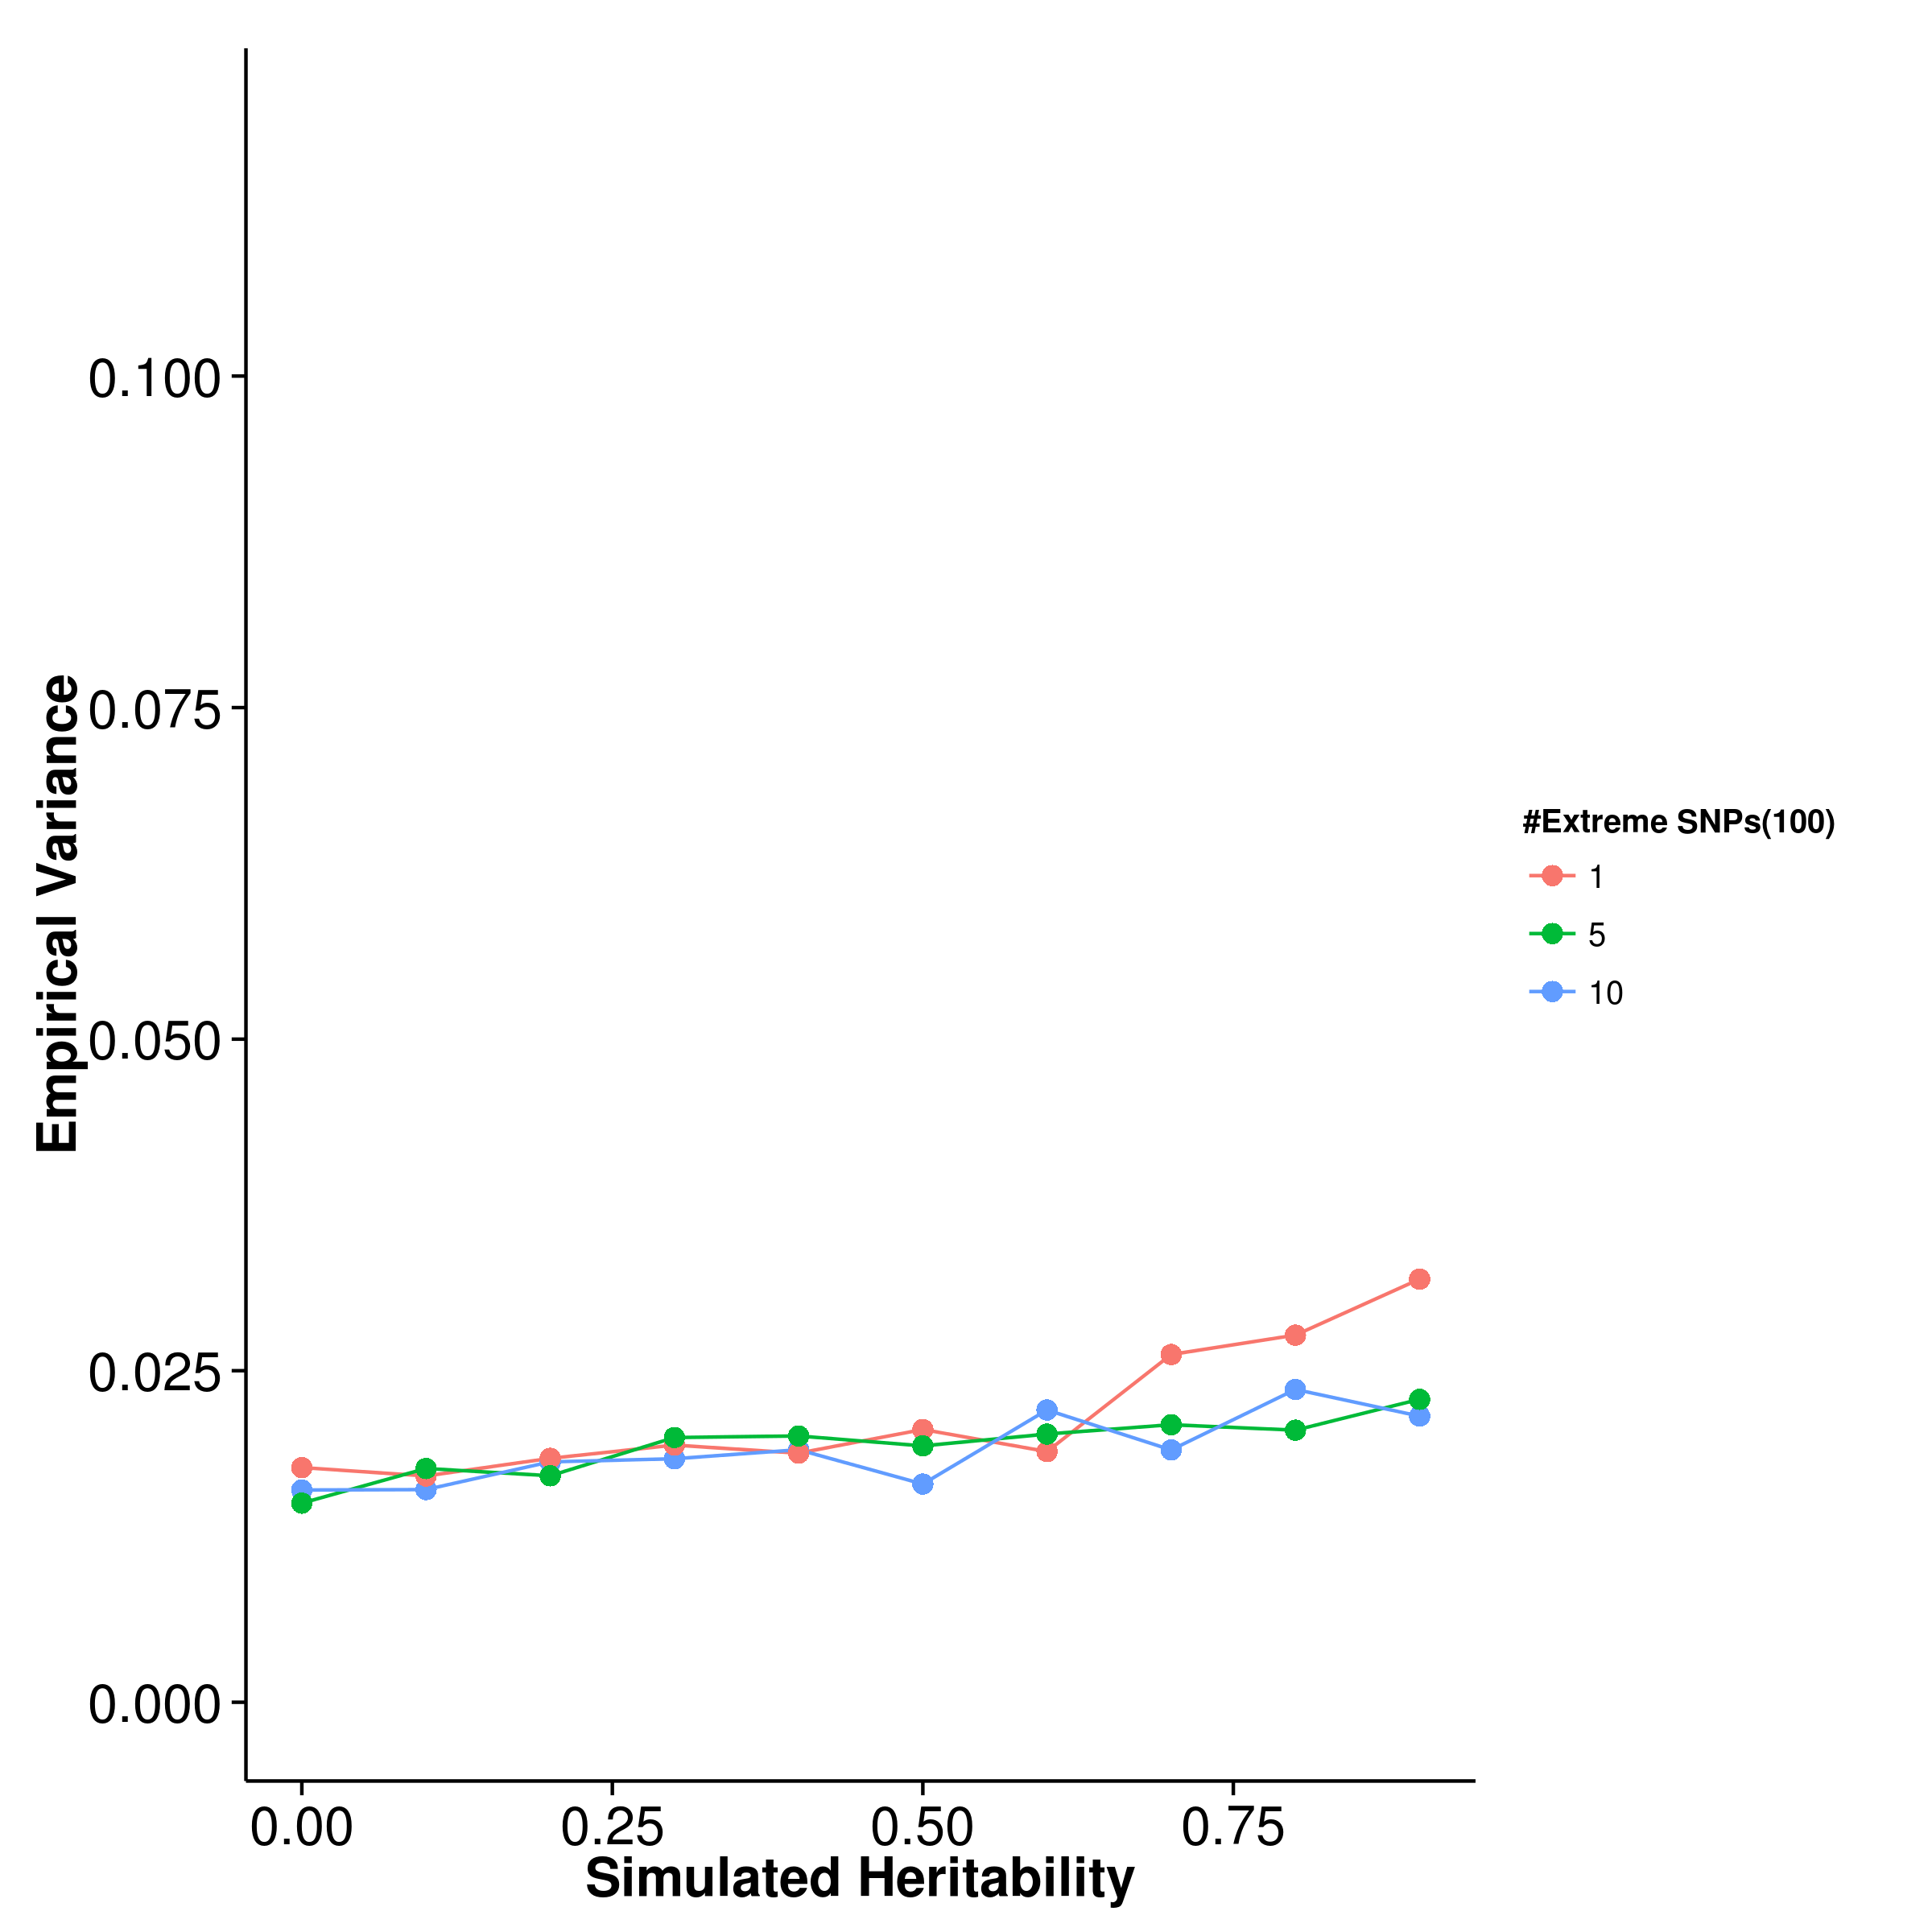
\includegraphics{figure/he_summary/extreme_100c/shrek_QtE_Rand_sd.png}}
				\label{fig:shrekQtEx100cVar}
			}
			\subfloat[GCTA]{
				\scalebox{.4}{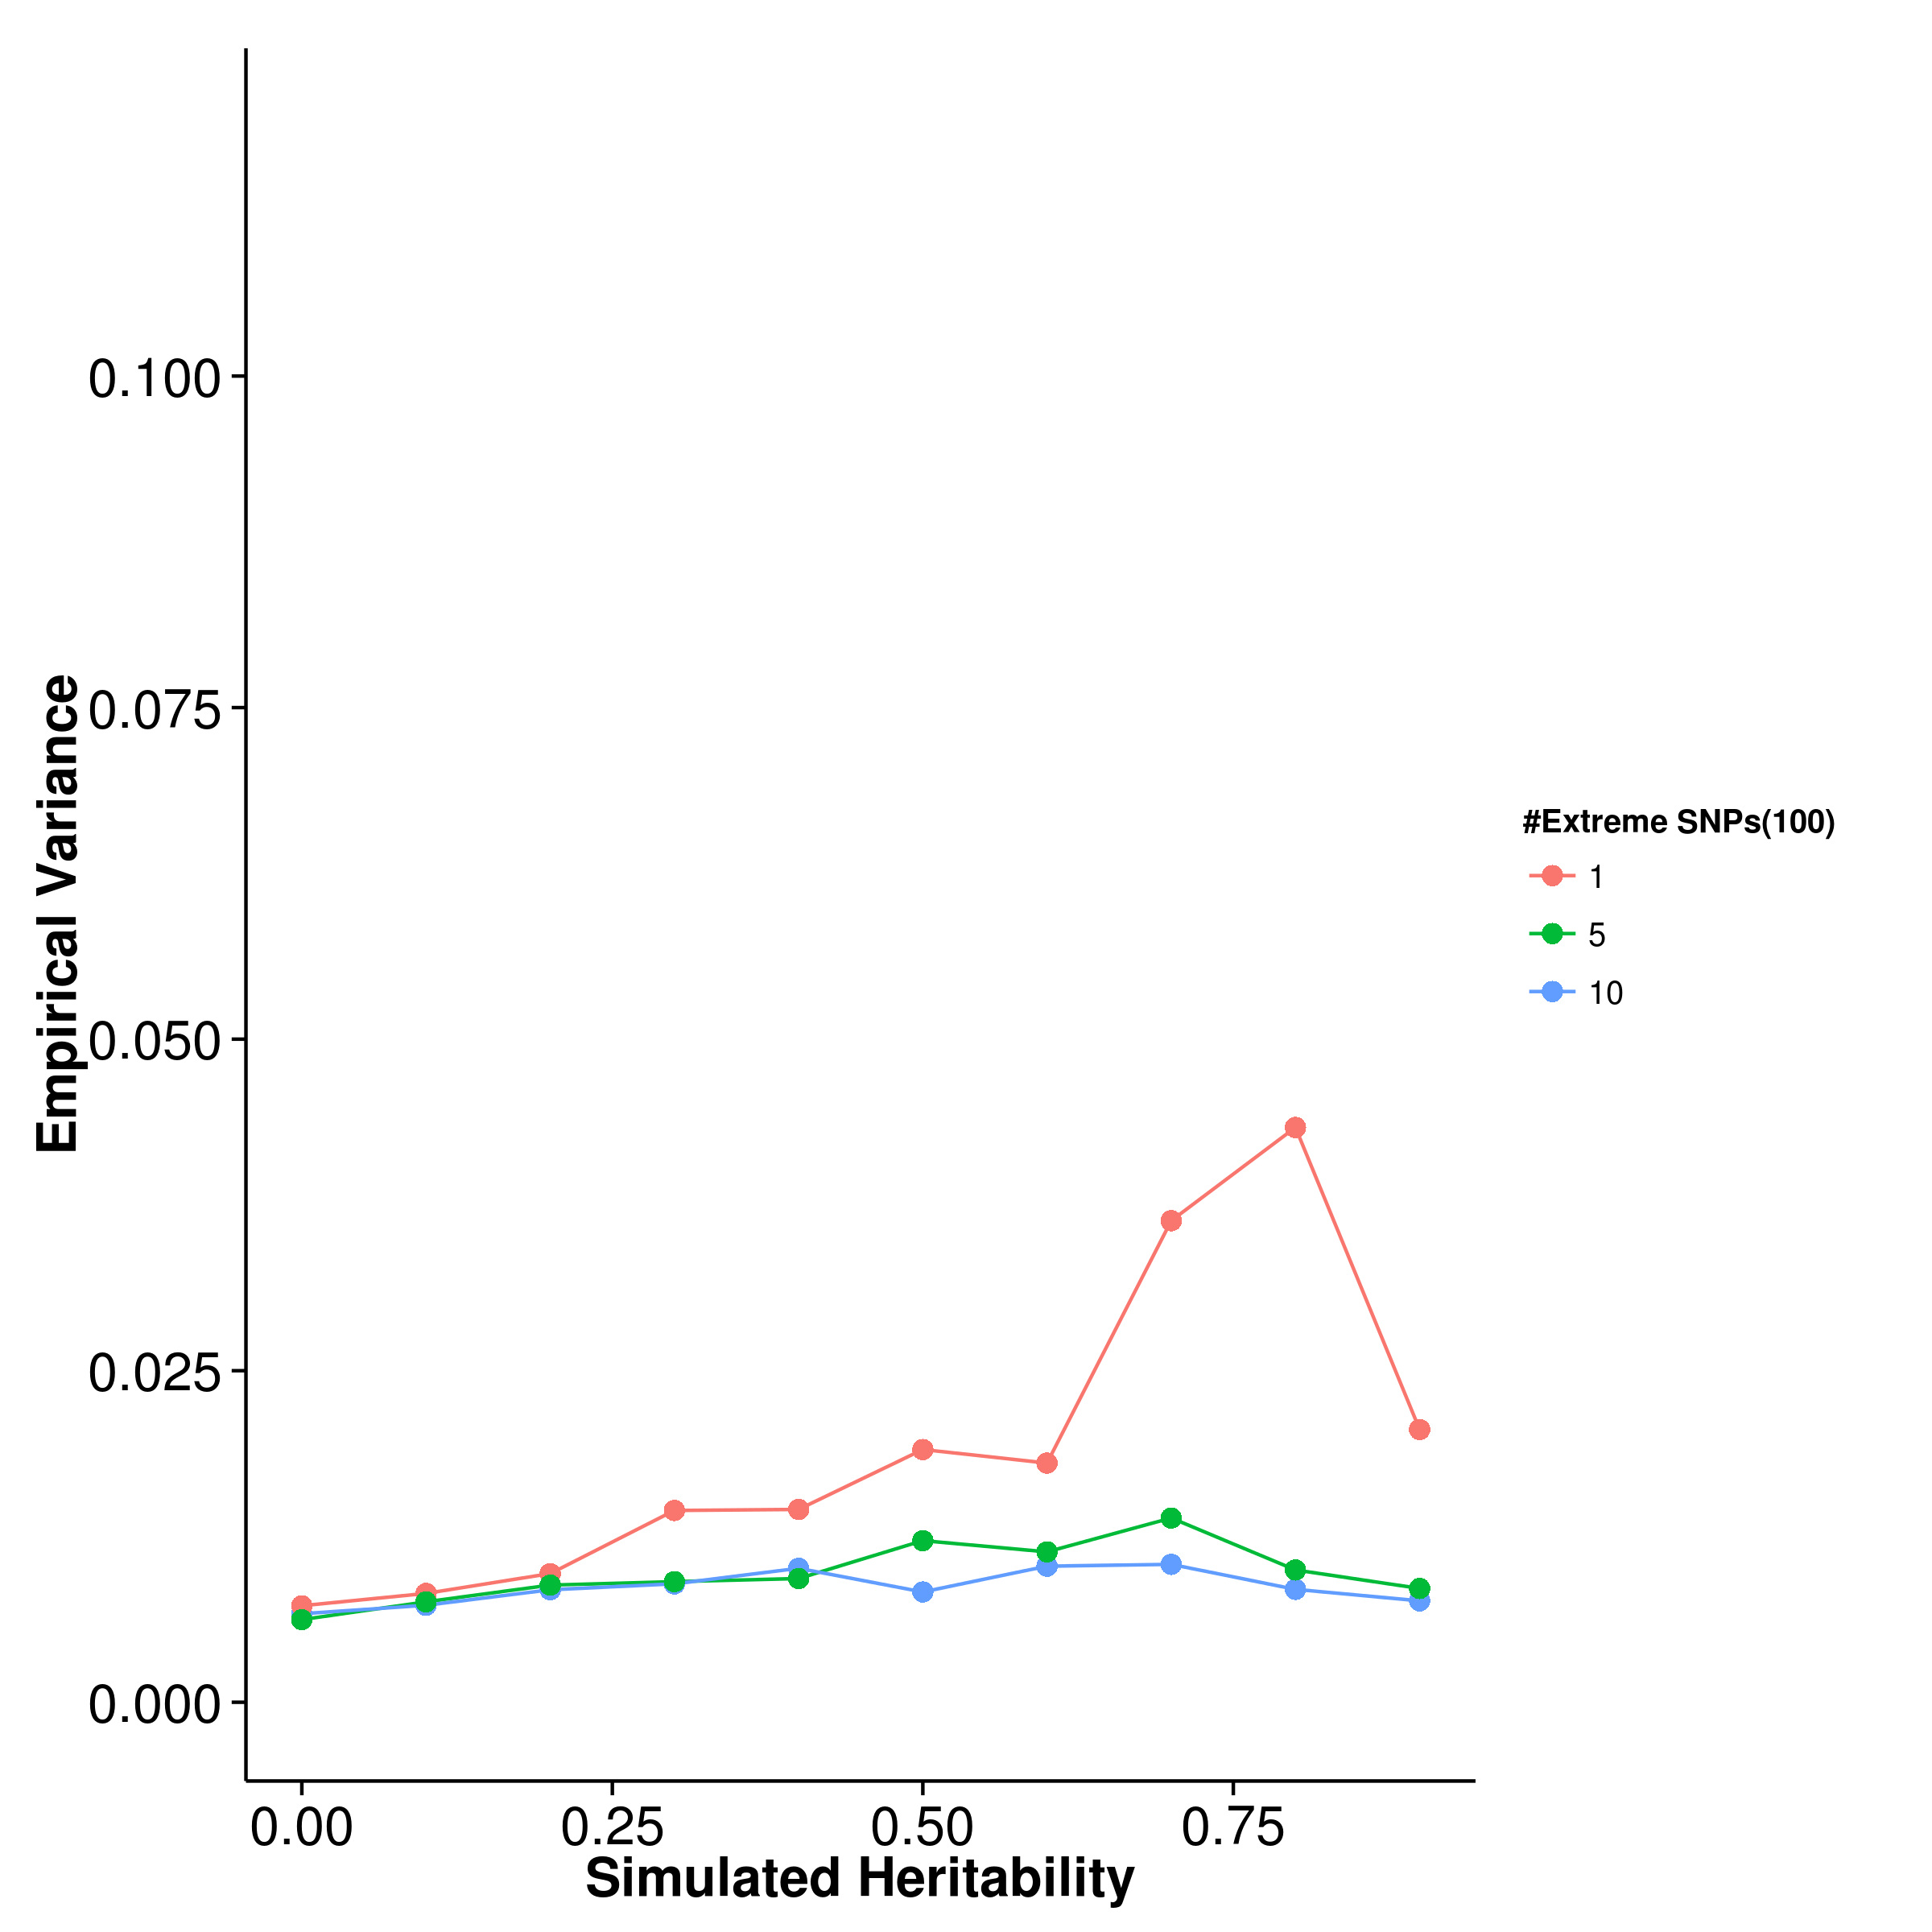
\includegraphics{figure/he_summary/extreme_100c/gcta_QtE_Rand_sd.png}}
				\label{fig:gctaQtEx100cVar}
			}\\
			\subfloat[LDSC with fix intercept]{
				\scalebox{.4}{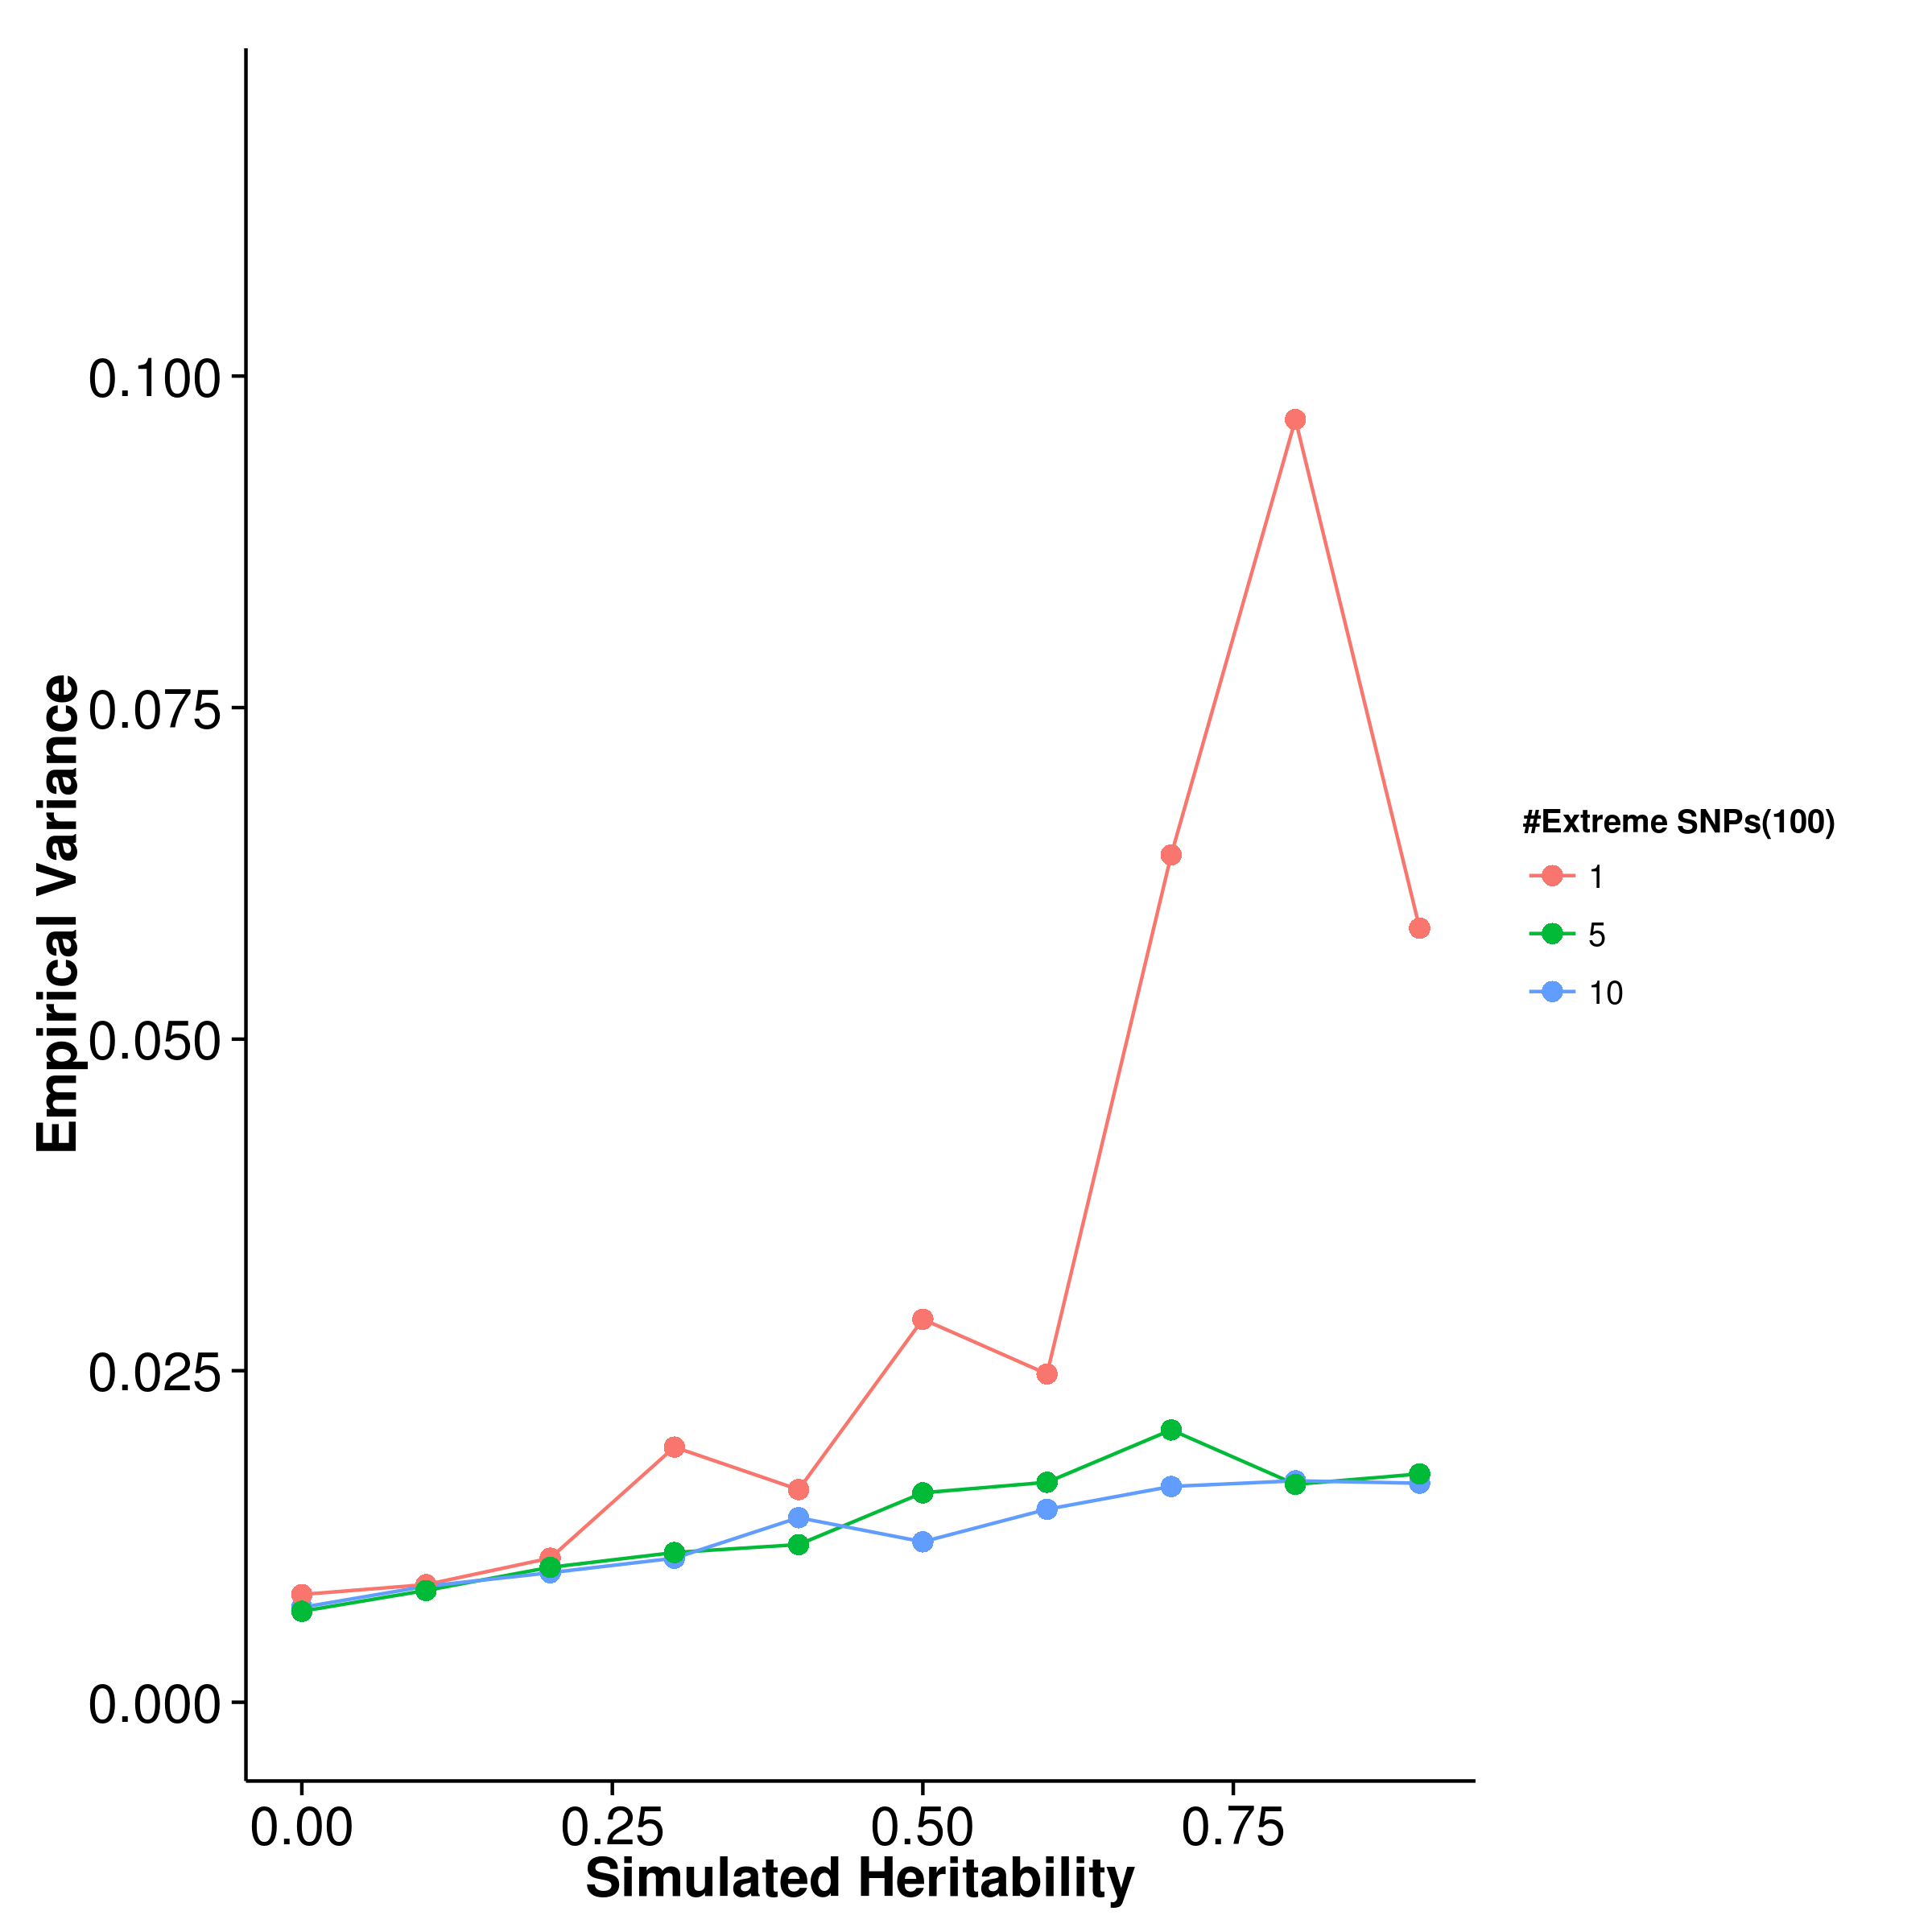
\includegraphics{figure/he_summary/extreme_100c/ldsc_QtE_Rand_sd.png}}
				\label{fig:ldscQtEx100cVar}
			}
			\subfloat[LDSC with intercept estimation]{
				
				\scalebox{.4}{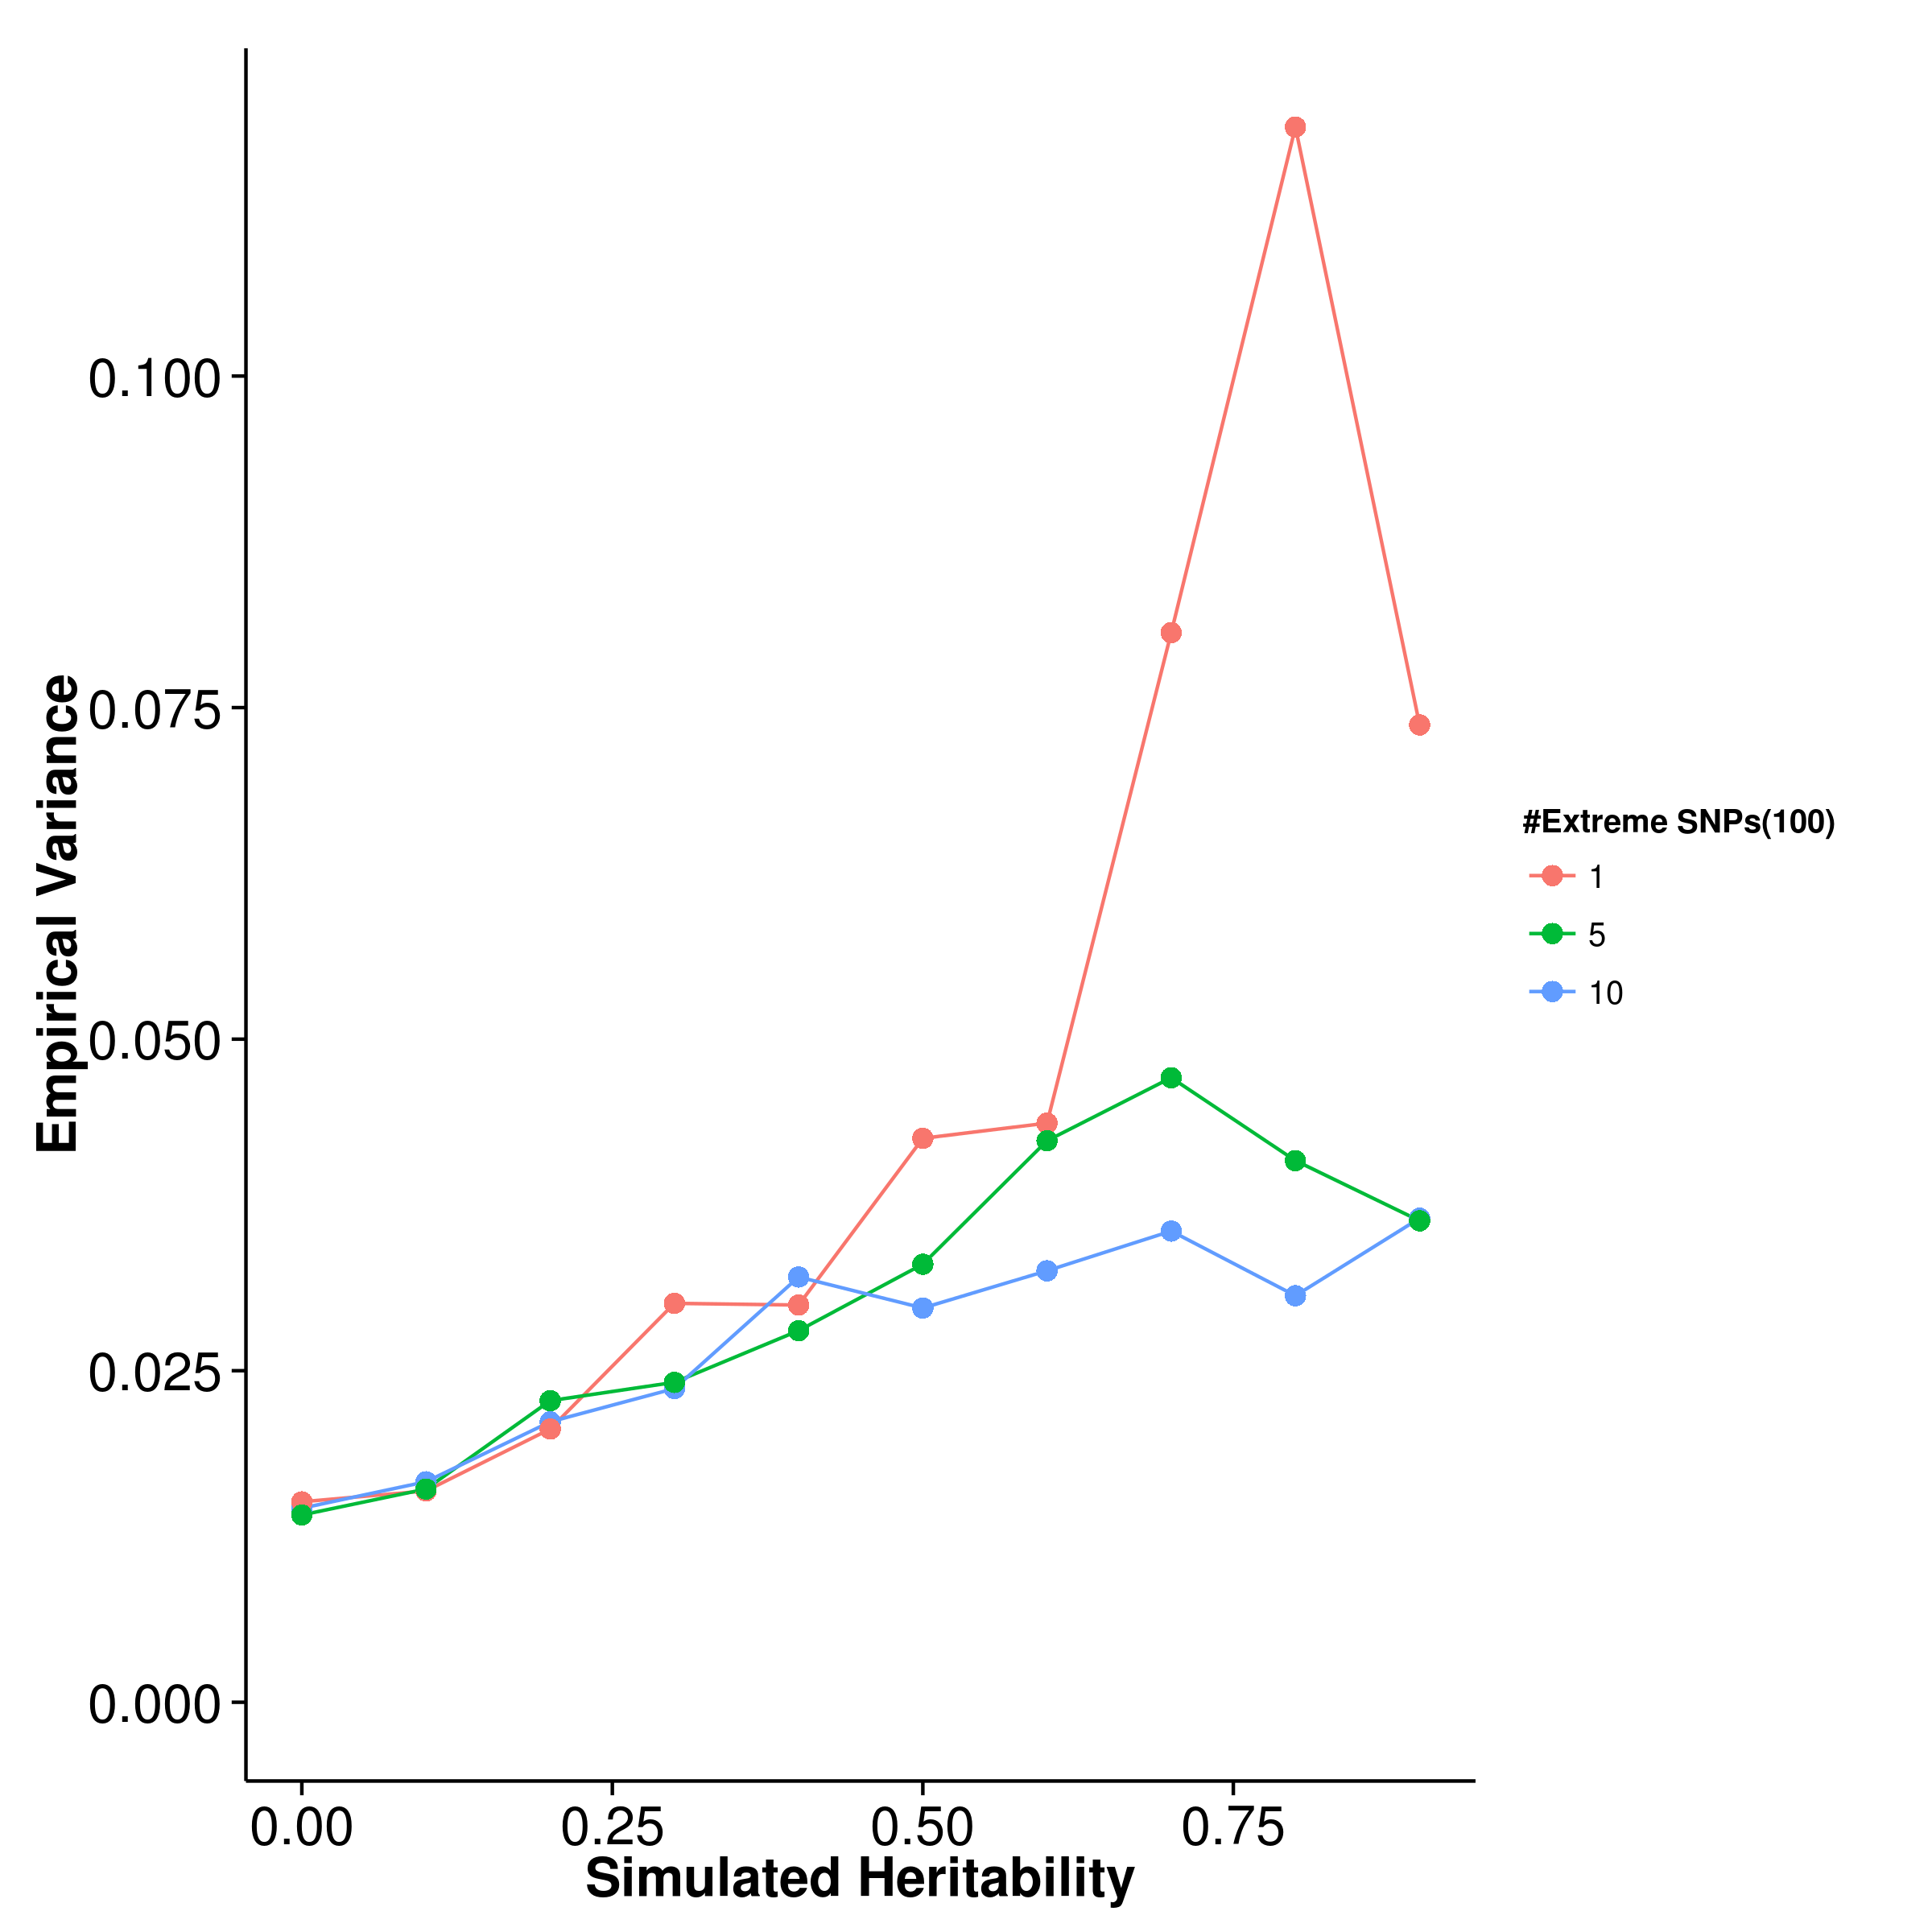
\includegraphics{figure/he_summary/extreme_100c/ldscIn_QtE_Rand_sd.png}}
				\label{fig:ldscInQtEx100cVar}
			}
			\caption[Variance of Extreme Effect Size Simulation Result]
			{Variance of results from quantitative trait simulation with extreme effect size simulation.
				100 causal \glspl{SNP} were simulated.
				When only 1 \gls{SNP} with extreme effect was simulated, the empirical variance of \gls{gcta} and \gls{ldsc} increases and a large fluctuation was observed.
				Whereas the empirical variance of \gls{shrek} only increase slightly when the simulated heritability is large and with only 1 \gls{SNP} with extreme effect.
				Suggesting that it is more robust to the change in number of extreme \gls{SNP}(s).
			} 
			\label{fig:QtEx100cVar}
		\end{figure}
		
		\begin{figure}
			\centering
			\subfloat[SHREK]{
				\scalebox{.4}{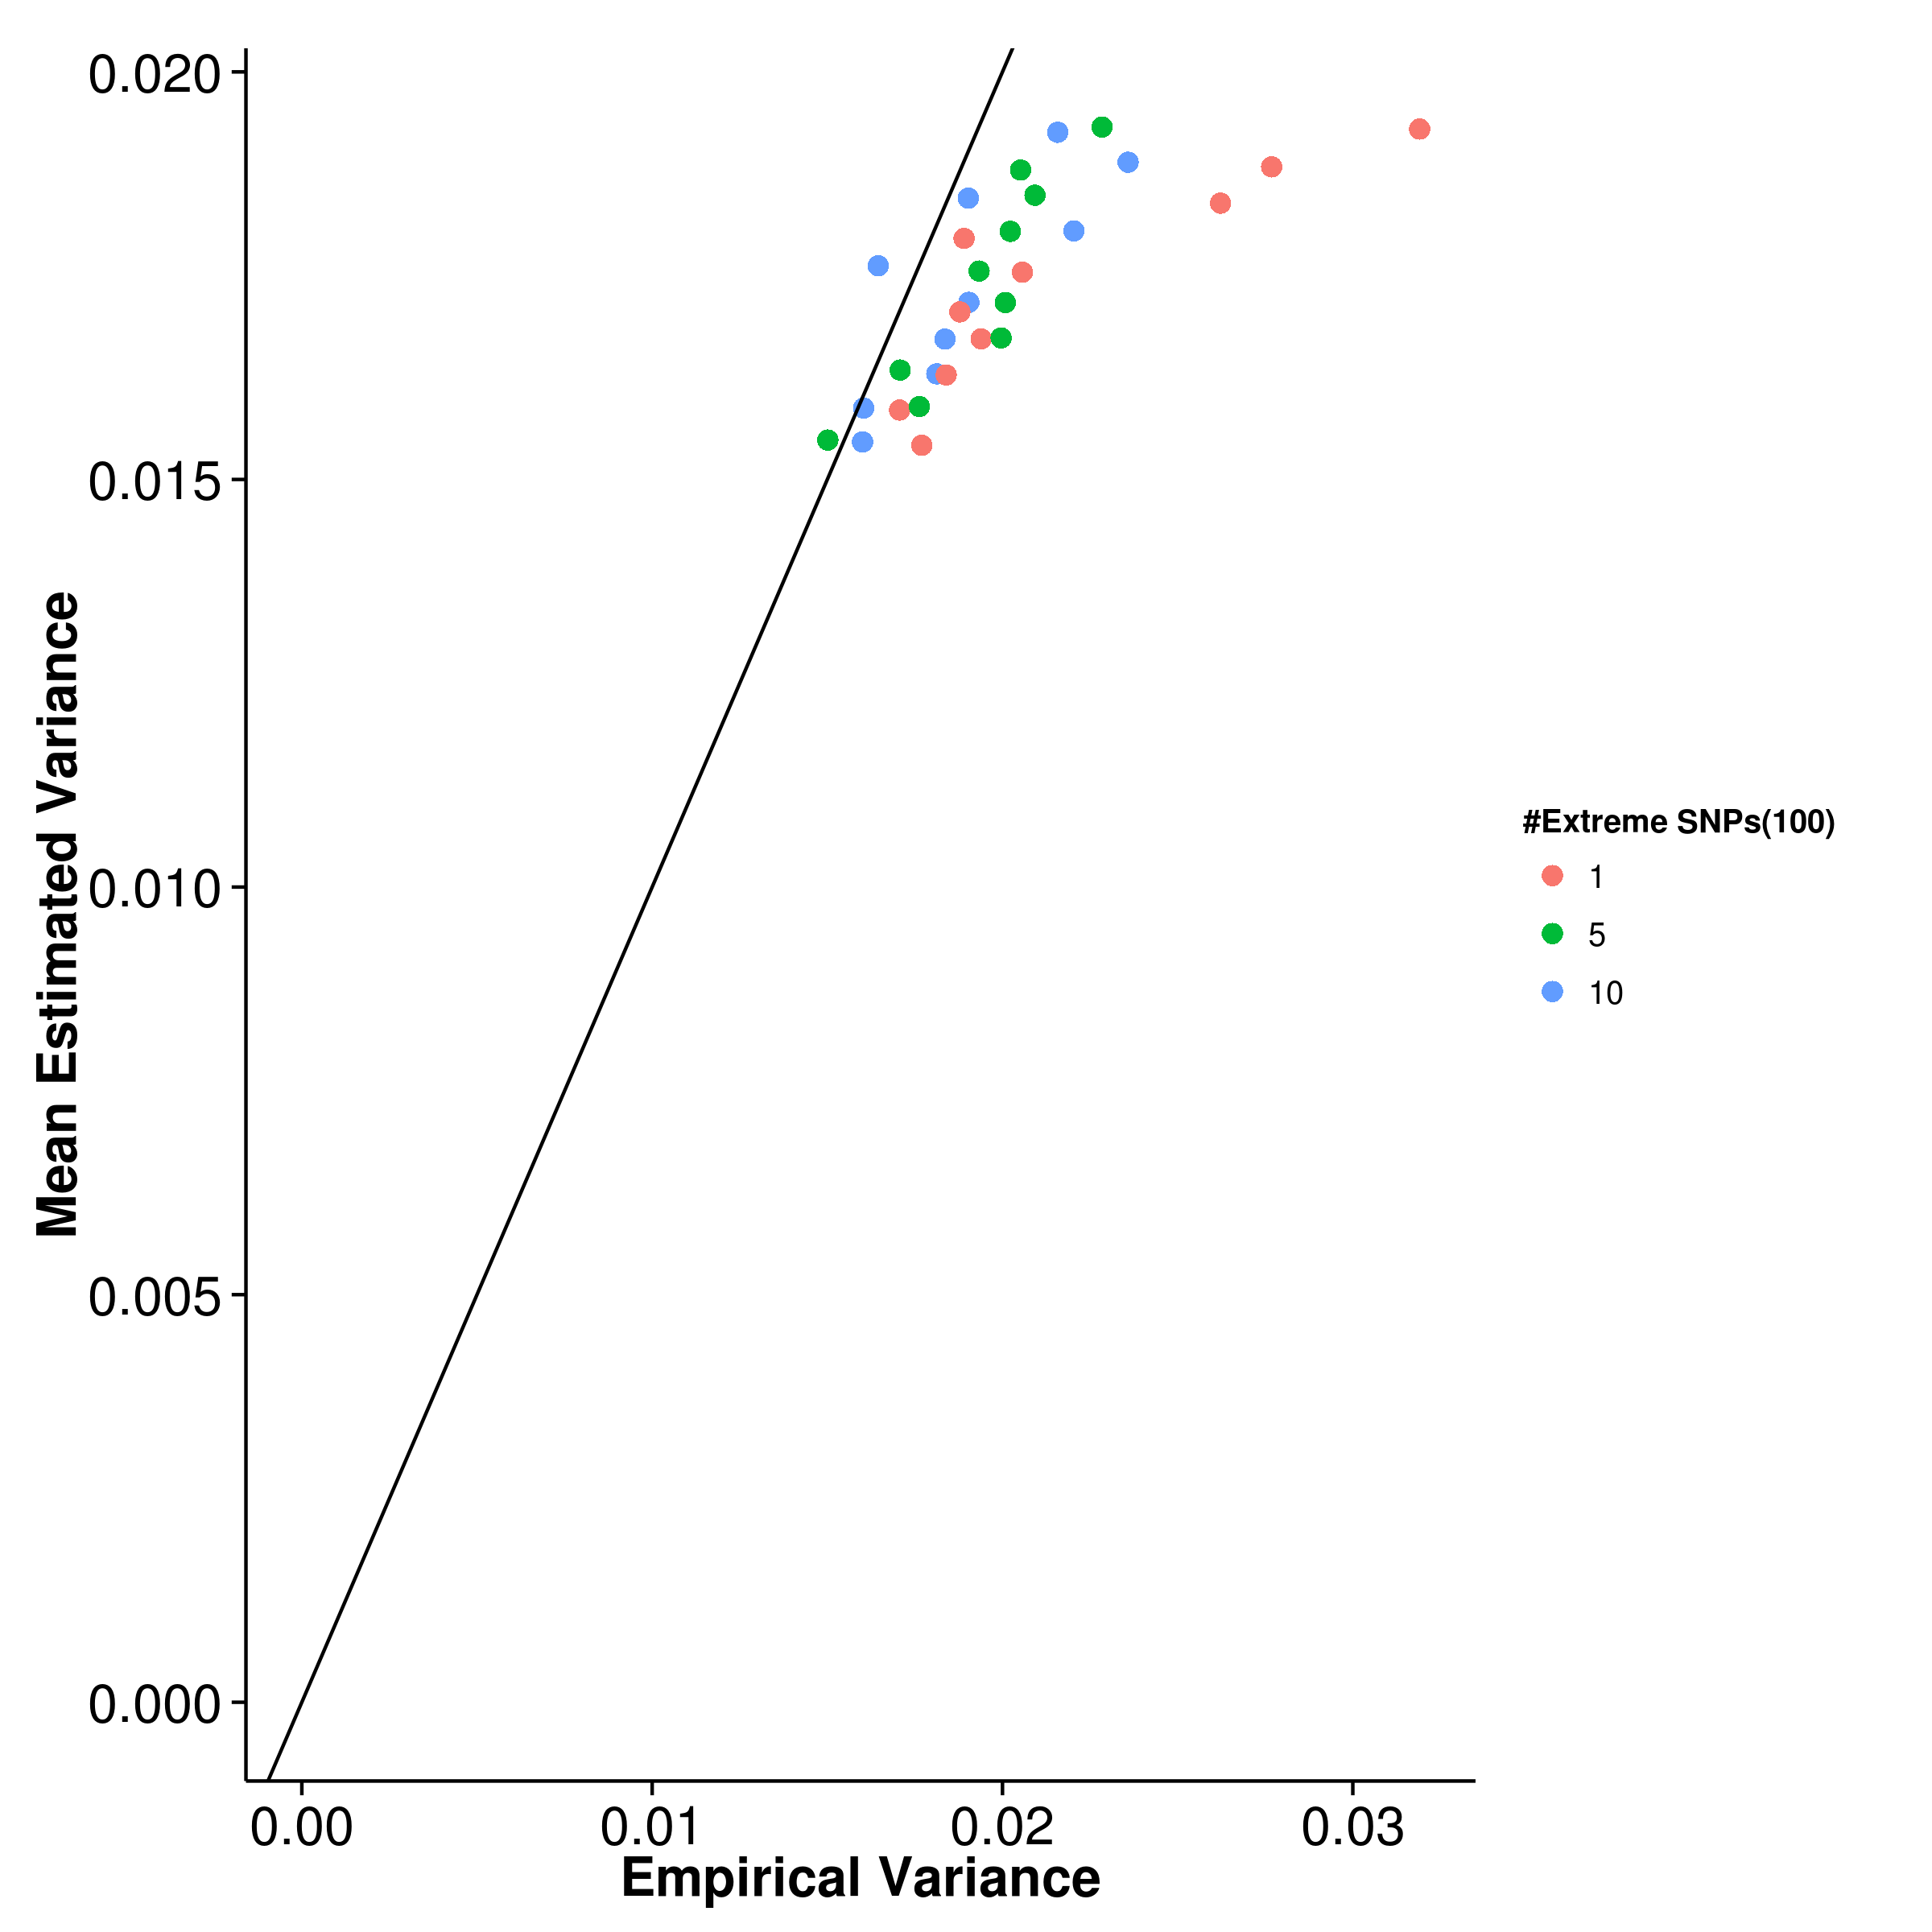
\includegraphics{figure/he_summary/extreme_100c/shrek_QtE_Rand_sdCom.png}}
				\label{fig:shrekQtEx100cVarCom}
			}
			\subfloat[GCTA]{
				\scalebox{.4}{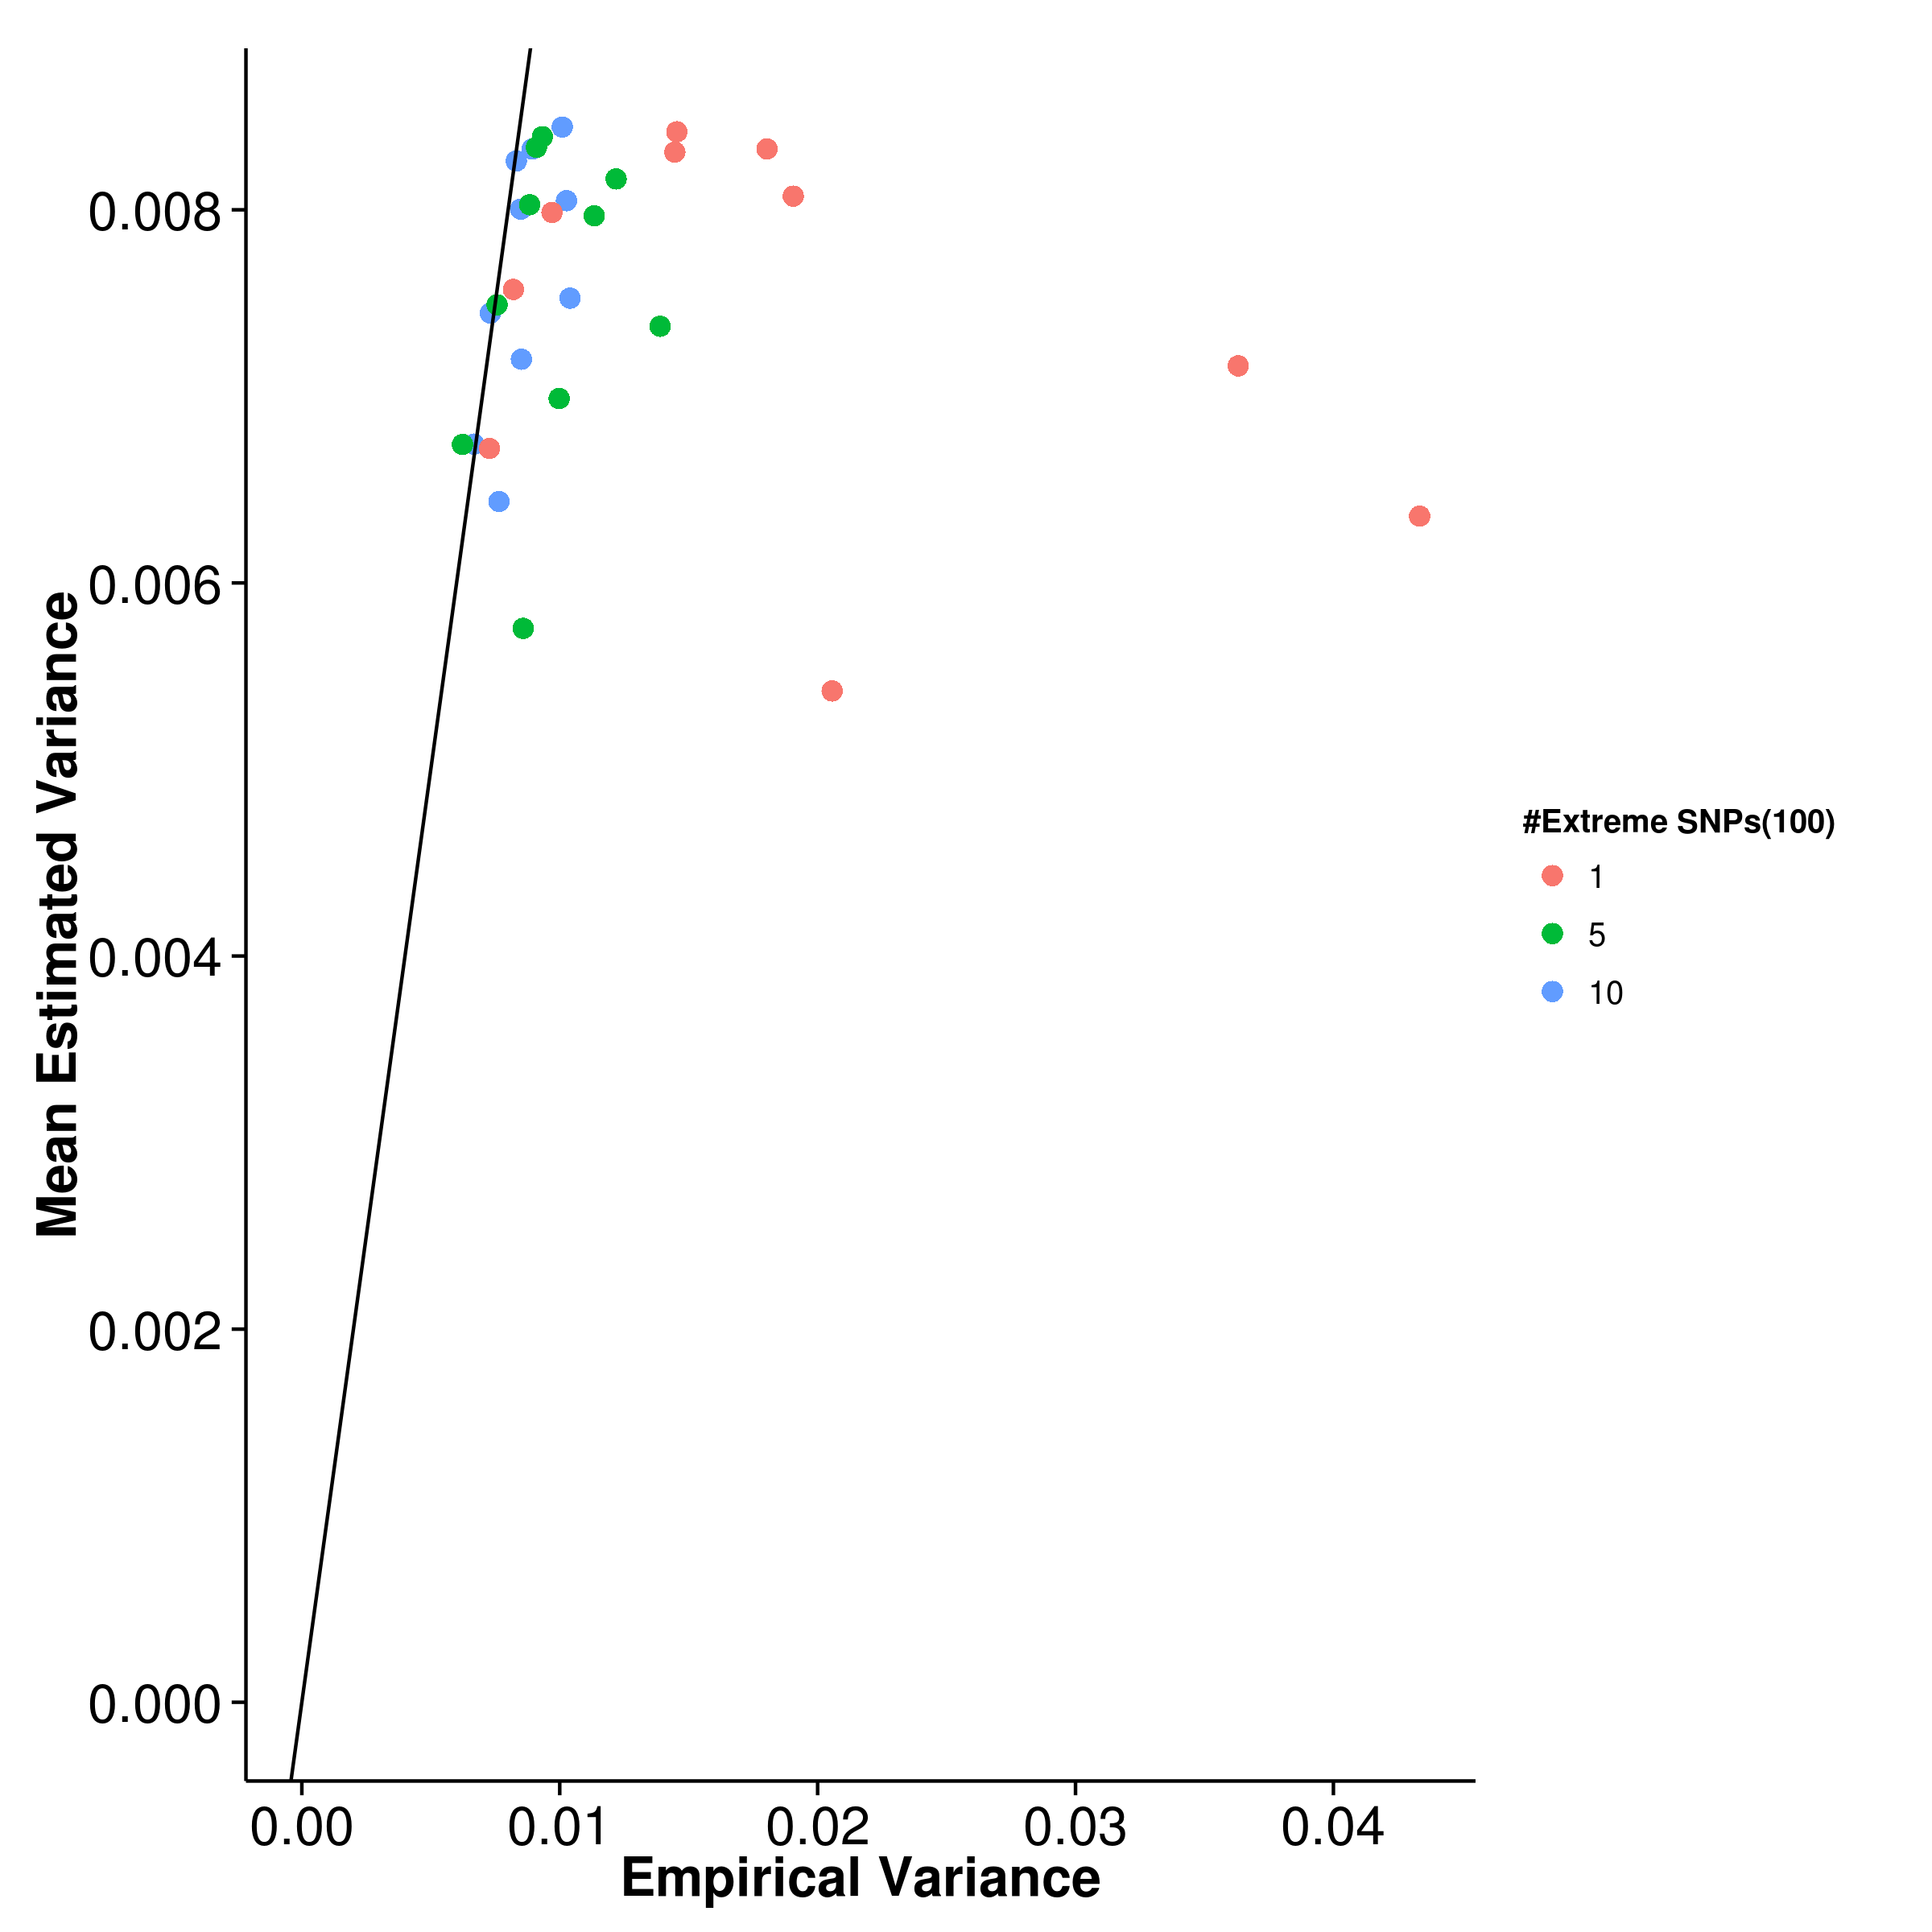
\includegraphics{figure/he_summary/extreme_100c/gcta_QtE_Rand_sdCom.png}}
				\label{fig:gctaQtEx100cVarCom}
			}\\
			\subfloat[LDSC with fix intercept]{
				\scalebox{.4}{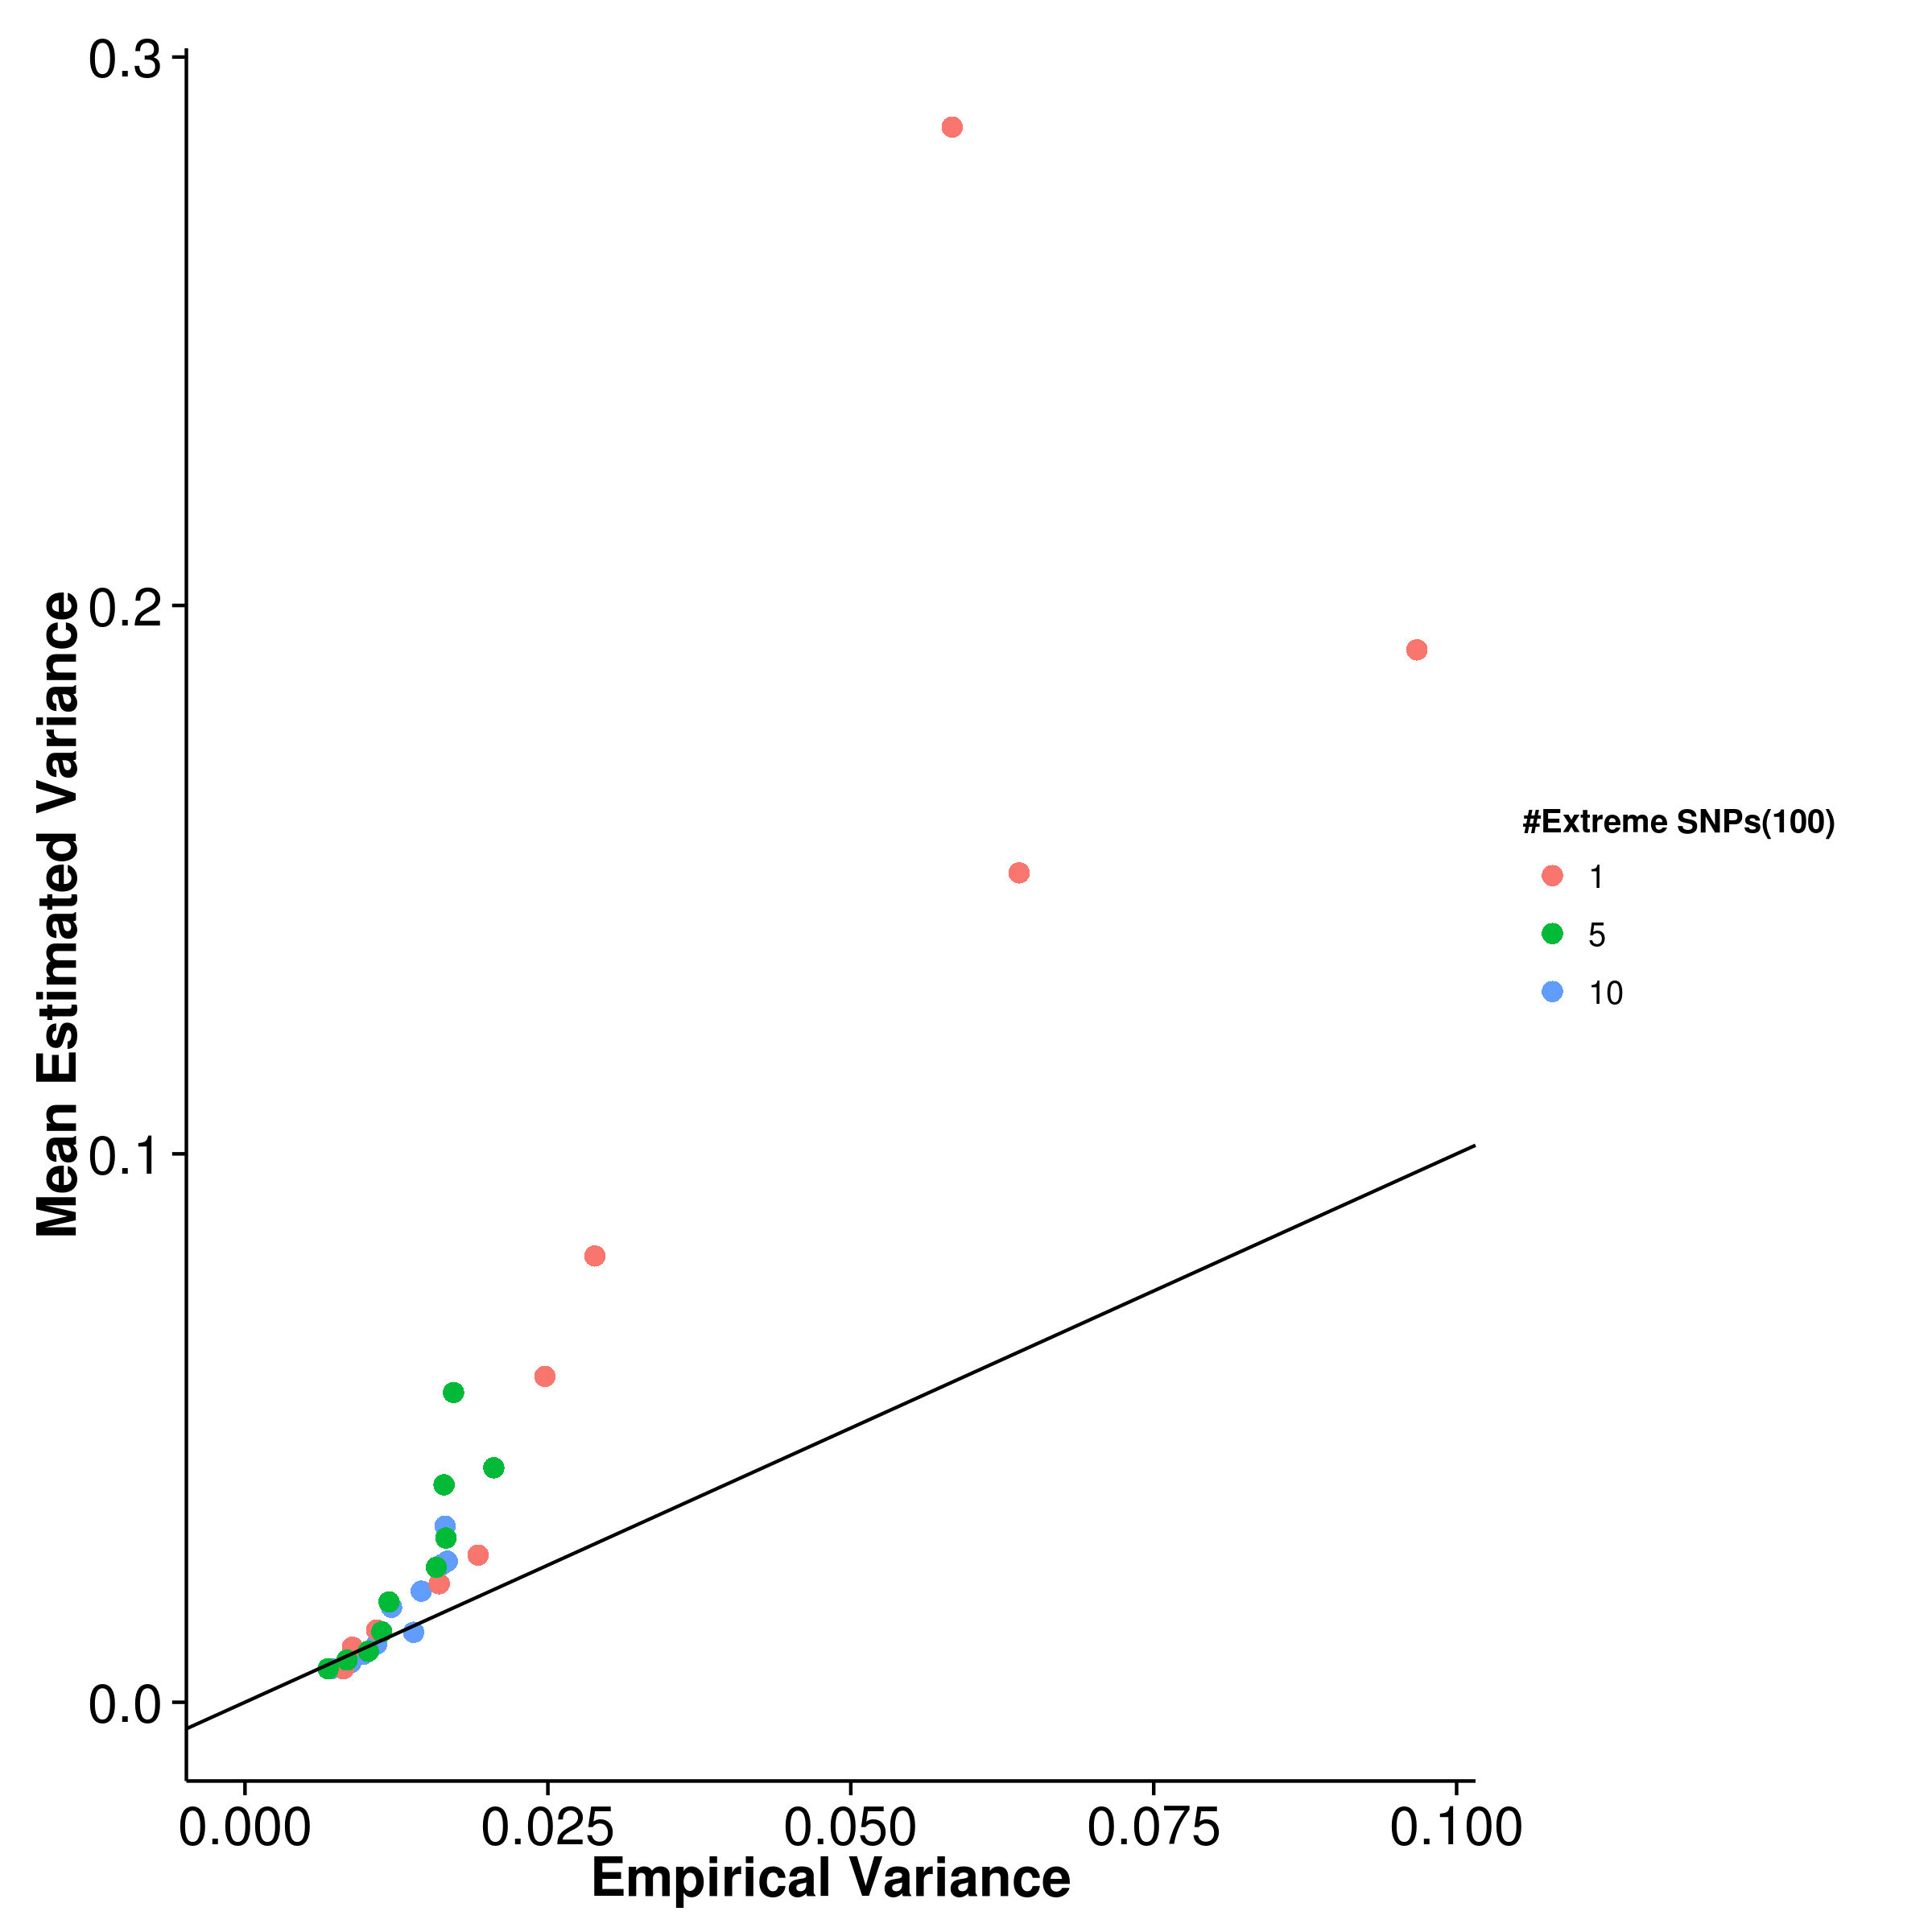
\includegraphics{figure/he_summary/extreme_100c/ldsc_QtE_Rand_sdCom.png}}
				\label{fig:ldscQtEx100cVarCom}
			}
			\subfloat[LDSC with intercept estimation]{
				
				\scalebox{.4}{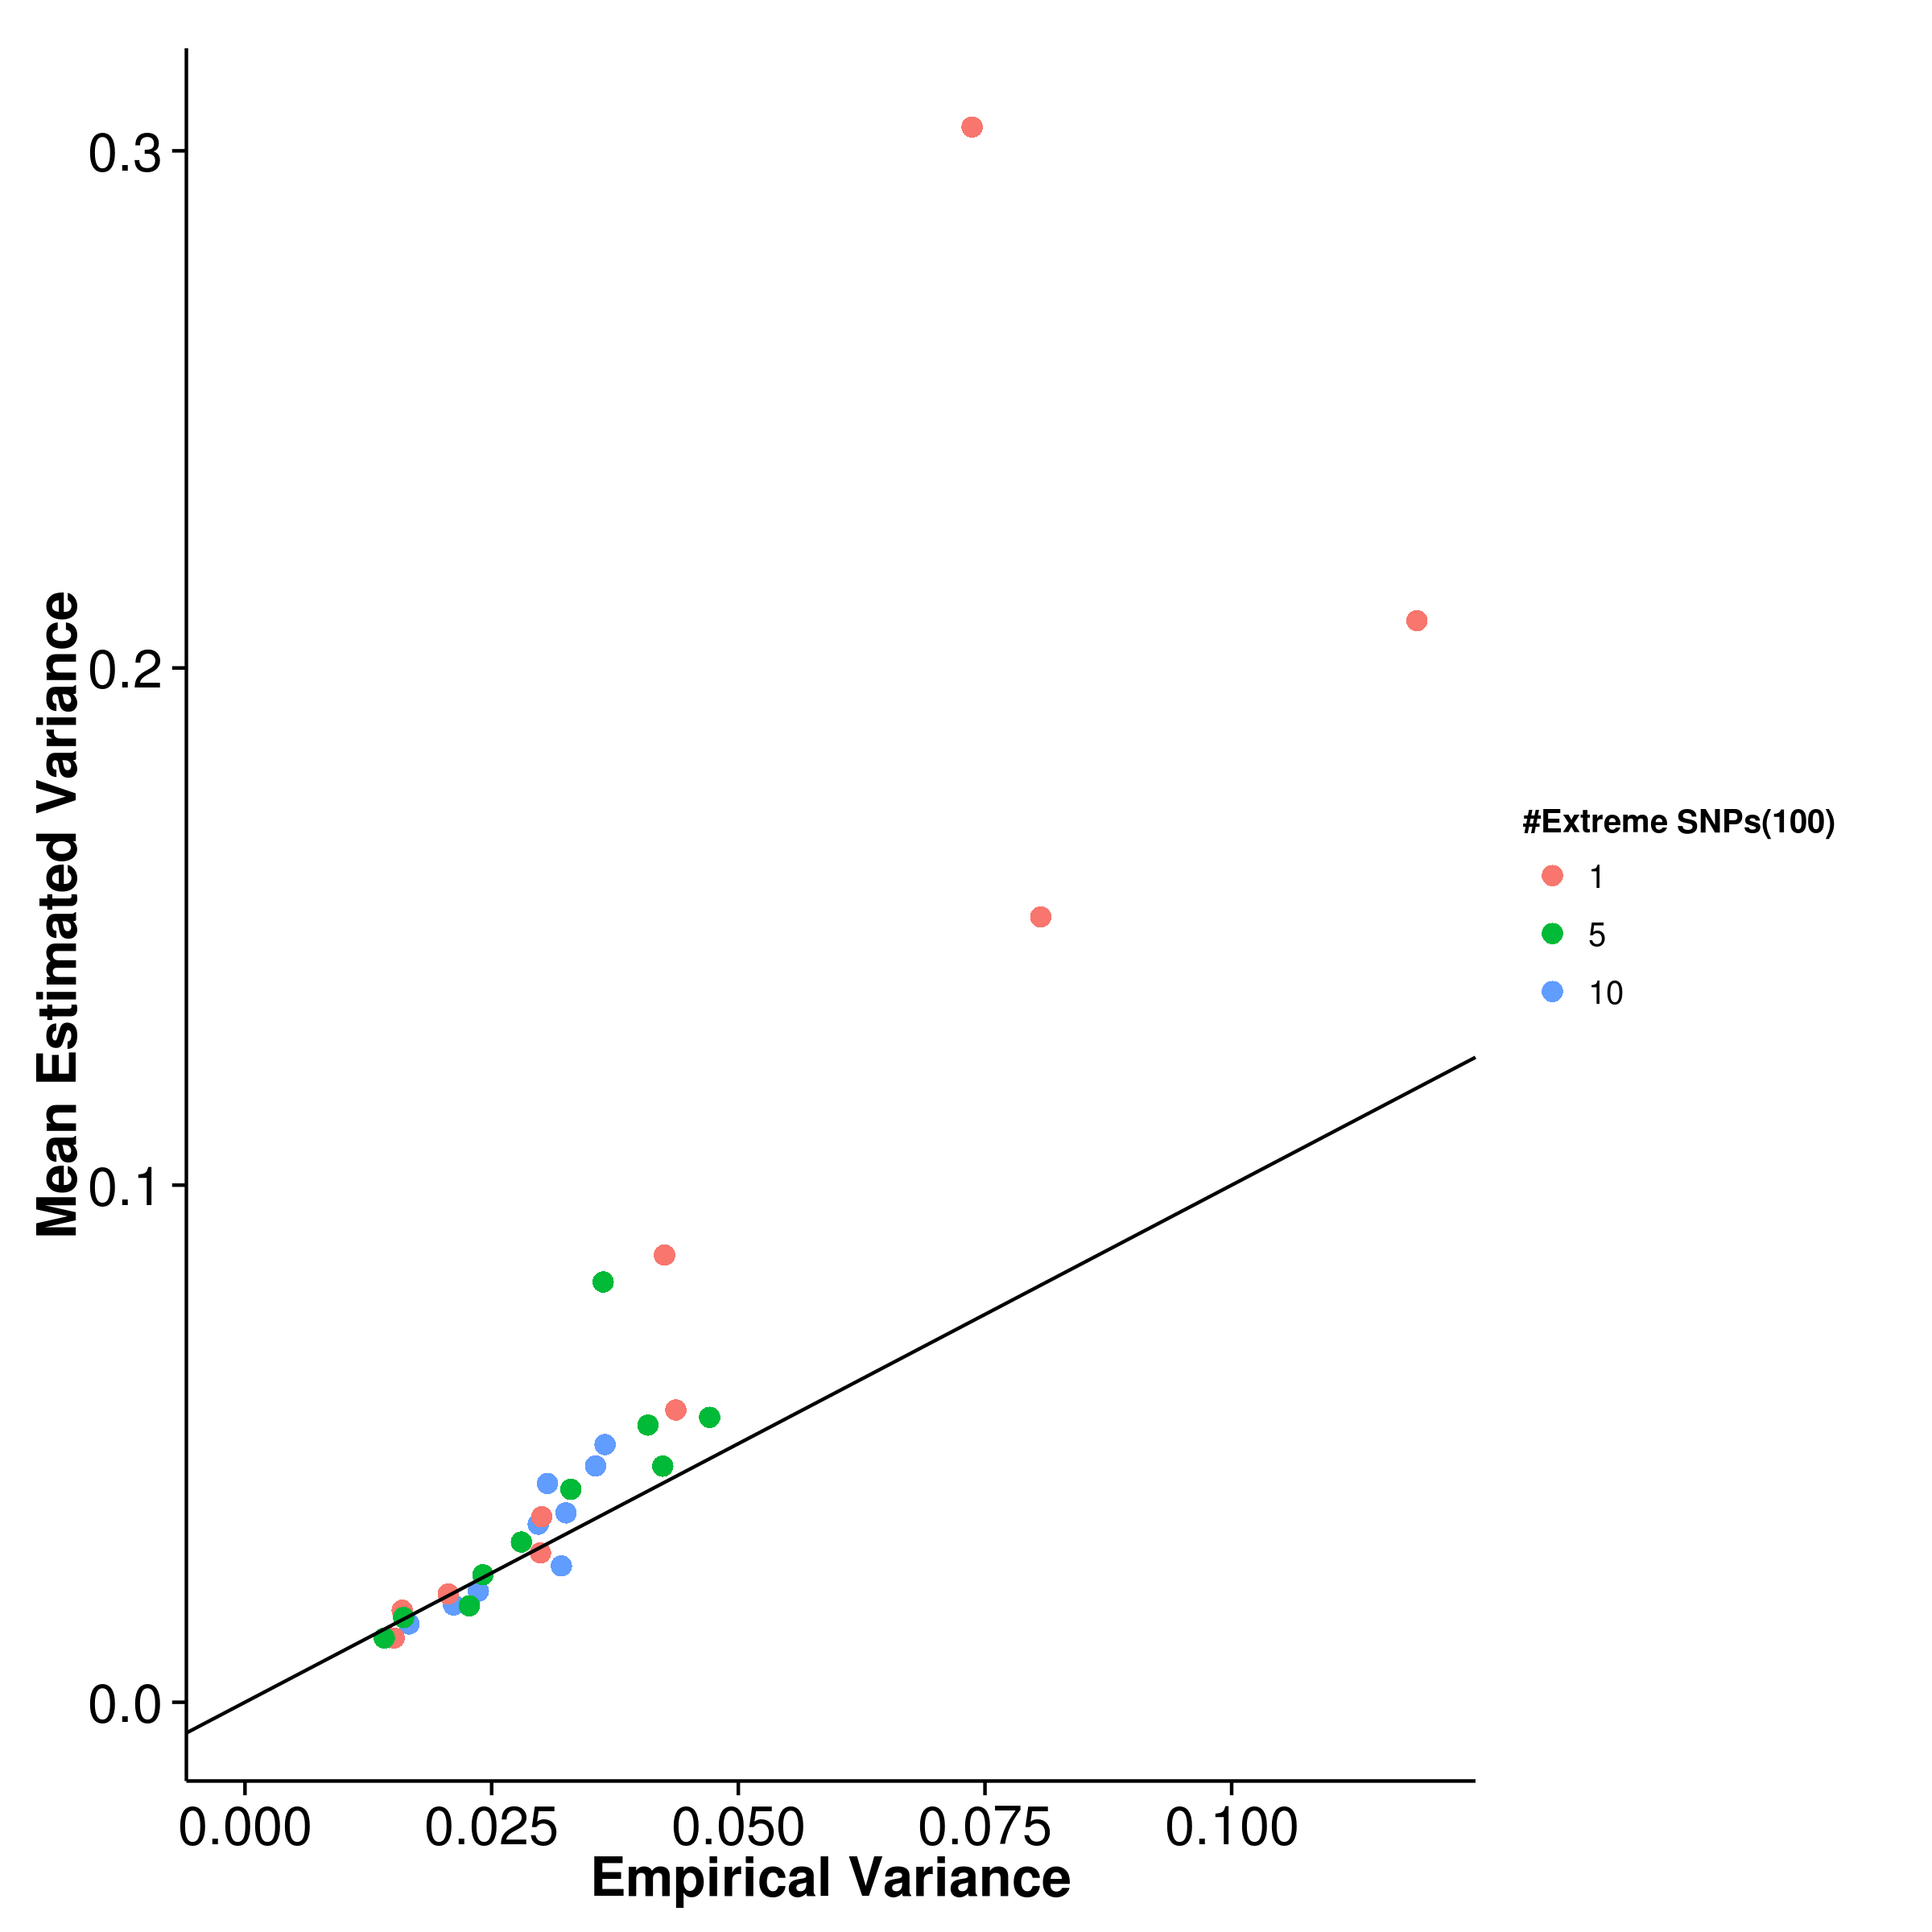
\includegraphics{figure/he_summary/extreme_100c/ldscIn_QtE_Rand_sdCom.png}}
				\label{fig:ldscInQtEx100cVarCom}
			}
			\caption[Estimation of Variance in Extreme Effect Size Simulation]
			{Estimated variance of results from quantitative trait simulation with extreme effect size simulation when compared to the empirical variance.
				100 causal \glspl{SNP} were simulated.
				\gls{shrek} and \gls{gcta} generally under-estimate the variance with the magnitude of bias being the highest when there is only 1 \gls{SNP} with extreme effect.
				On the other hand, \gls{ldsc} tends to over-estimate the variance and it can overestimate the variance by more than 3 folds when there is only 1 \gls{SNP} with extreme effect.
			} 
			\label{fig:QtEx100cVarCom}
		\end{figure}
		Similarly, we were interested in the performance of the algorithms when a small number of \glspl{SNP} account for majority of the effect. 
		In this simulation, we simulated 100 causal \glspl{SNP} of which 1, 5 or 10 of those \glspl{SNP} account for majority of the effects.
		
		When assessing the mean estimation of heritability (\cref{fig:QtEx100cMean}), the performance of the algorithms were similar to that in the quantitative trait simulation.
		The only exception was when 1 \gls{SNP} account for majority of effects during which the bias of estimation fluctuates in most algorithms except \gls{shrek} (\cref{fig:shrekQtEx100cMean}). 
		Similarly, the variance of the estimation (\cref{fig:QtEx100cVar}) from \gls{gcta} and \gls{ldsc} increases when only 1 \gls{SNP} account for majority of effect.
		It was most obvious in the case of \gls{ldsc} where the variance increased drastically as the heritability is high (\cref{fig:ldscQtEx100cVar}).
		However, \gls{shrek} does not seems to be affected and were robust to the number of \glspl{SNP} with extreme effect. 
		
		The estimated variance of \gls{ldsc} were also affected by the number of \glspl{SNP} with extreme effect where a smaller number of extreme effect \glspl{SNP} the higher the estimated variance. 
		A similar bias was also observed in \gls{shrek} and \gls{gcta} where the estimated variance differ more form the empirical variance when the number of \glspl{SNP} with extreme effect is smaller. 
		
		To conclude, the performance of \gls{gcta} is superior to other algorithm except when there is 1 \gls{SNP} with extreme effect where \gls{shrek} performs better (\cref{tab:mseEx100c}).
		Again, the performance of \gls{shrek} was insensitive to the number of \glspl{SNP} with extreme effect.
		Performance of \gls{ldsc} gets better as the number of \glspl{SNP} with extreme effect increases and performance with fixed intercept is better than when the intercept estimation function was used. 
		 
		\begin{table}
			\centering
			\begin{tabular}{rrrrr}
				\toprule
				Number of Causal SNPs&	SHREK&	LDSC&	LDSC-In&	GCTA \\
				\midrule
				1	&	0.168	&	0.329	&	0.485	&	0.171\\
				5	&	0.158	&	0.208	&	0.340	&	0.0942\\
				10	&	0.155	&	0.179	&	0.334	&	0.0800\\
				\bottomrule
			\end{tabular}
			\caption[Mean Squared Error of Quantitative Trait Simulation with Extreme Effect Size]{
				\gls{mse} of quantitative trait simulation with extreme effect size.
				Of all the algorithms, \gls{gcta} has the lowest \gls{mse} except when there is only 1 \gls{SNP} with extreme effect.
				The performance of \gls{shrek} is in general better than \gls{ldsc} and the performance of \gls{shrek} and \gls{ldsc} with fixed intercept converges as the number of \glspl{SNP} with extreme effect increases.}
			\label{tab:mseEx100c}
		\end{table}
		
		% CC Rand Effect
		\subsection{Case Control Simulation}
			\begin{figure}
			\centering
			\subfloat[SHREK]{
				\scalebox{.4}{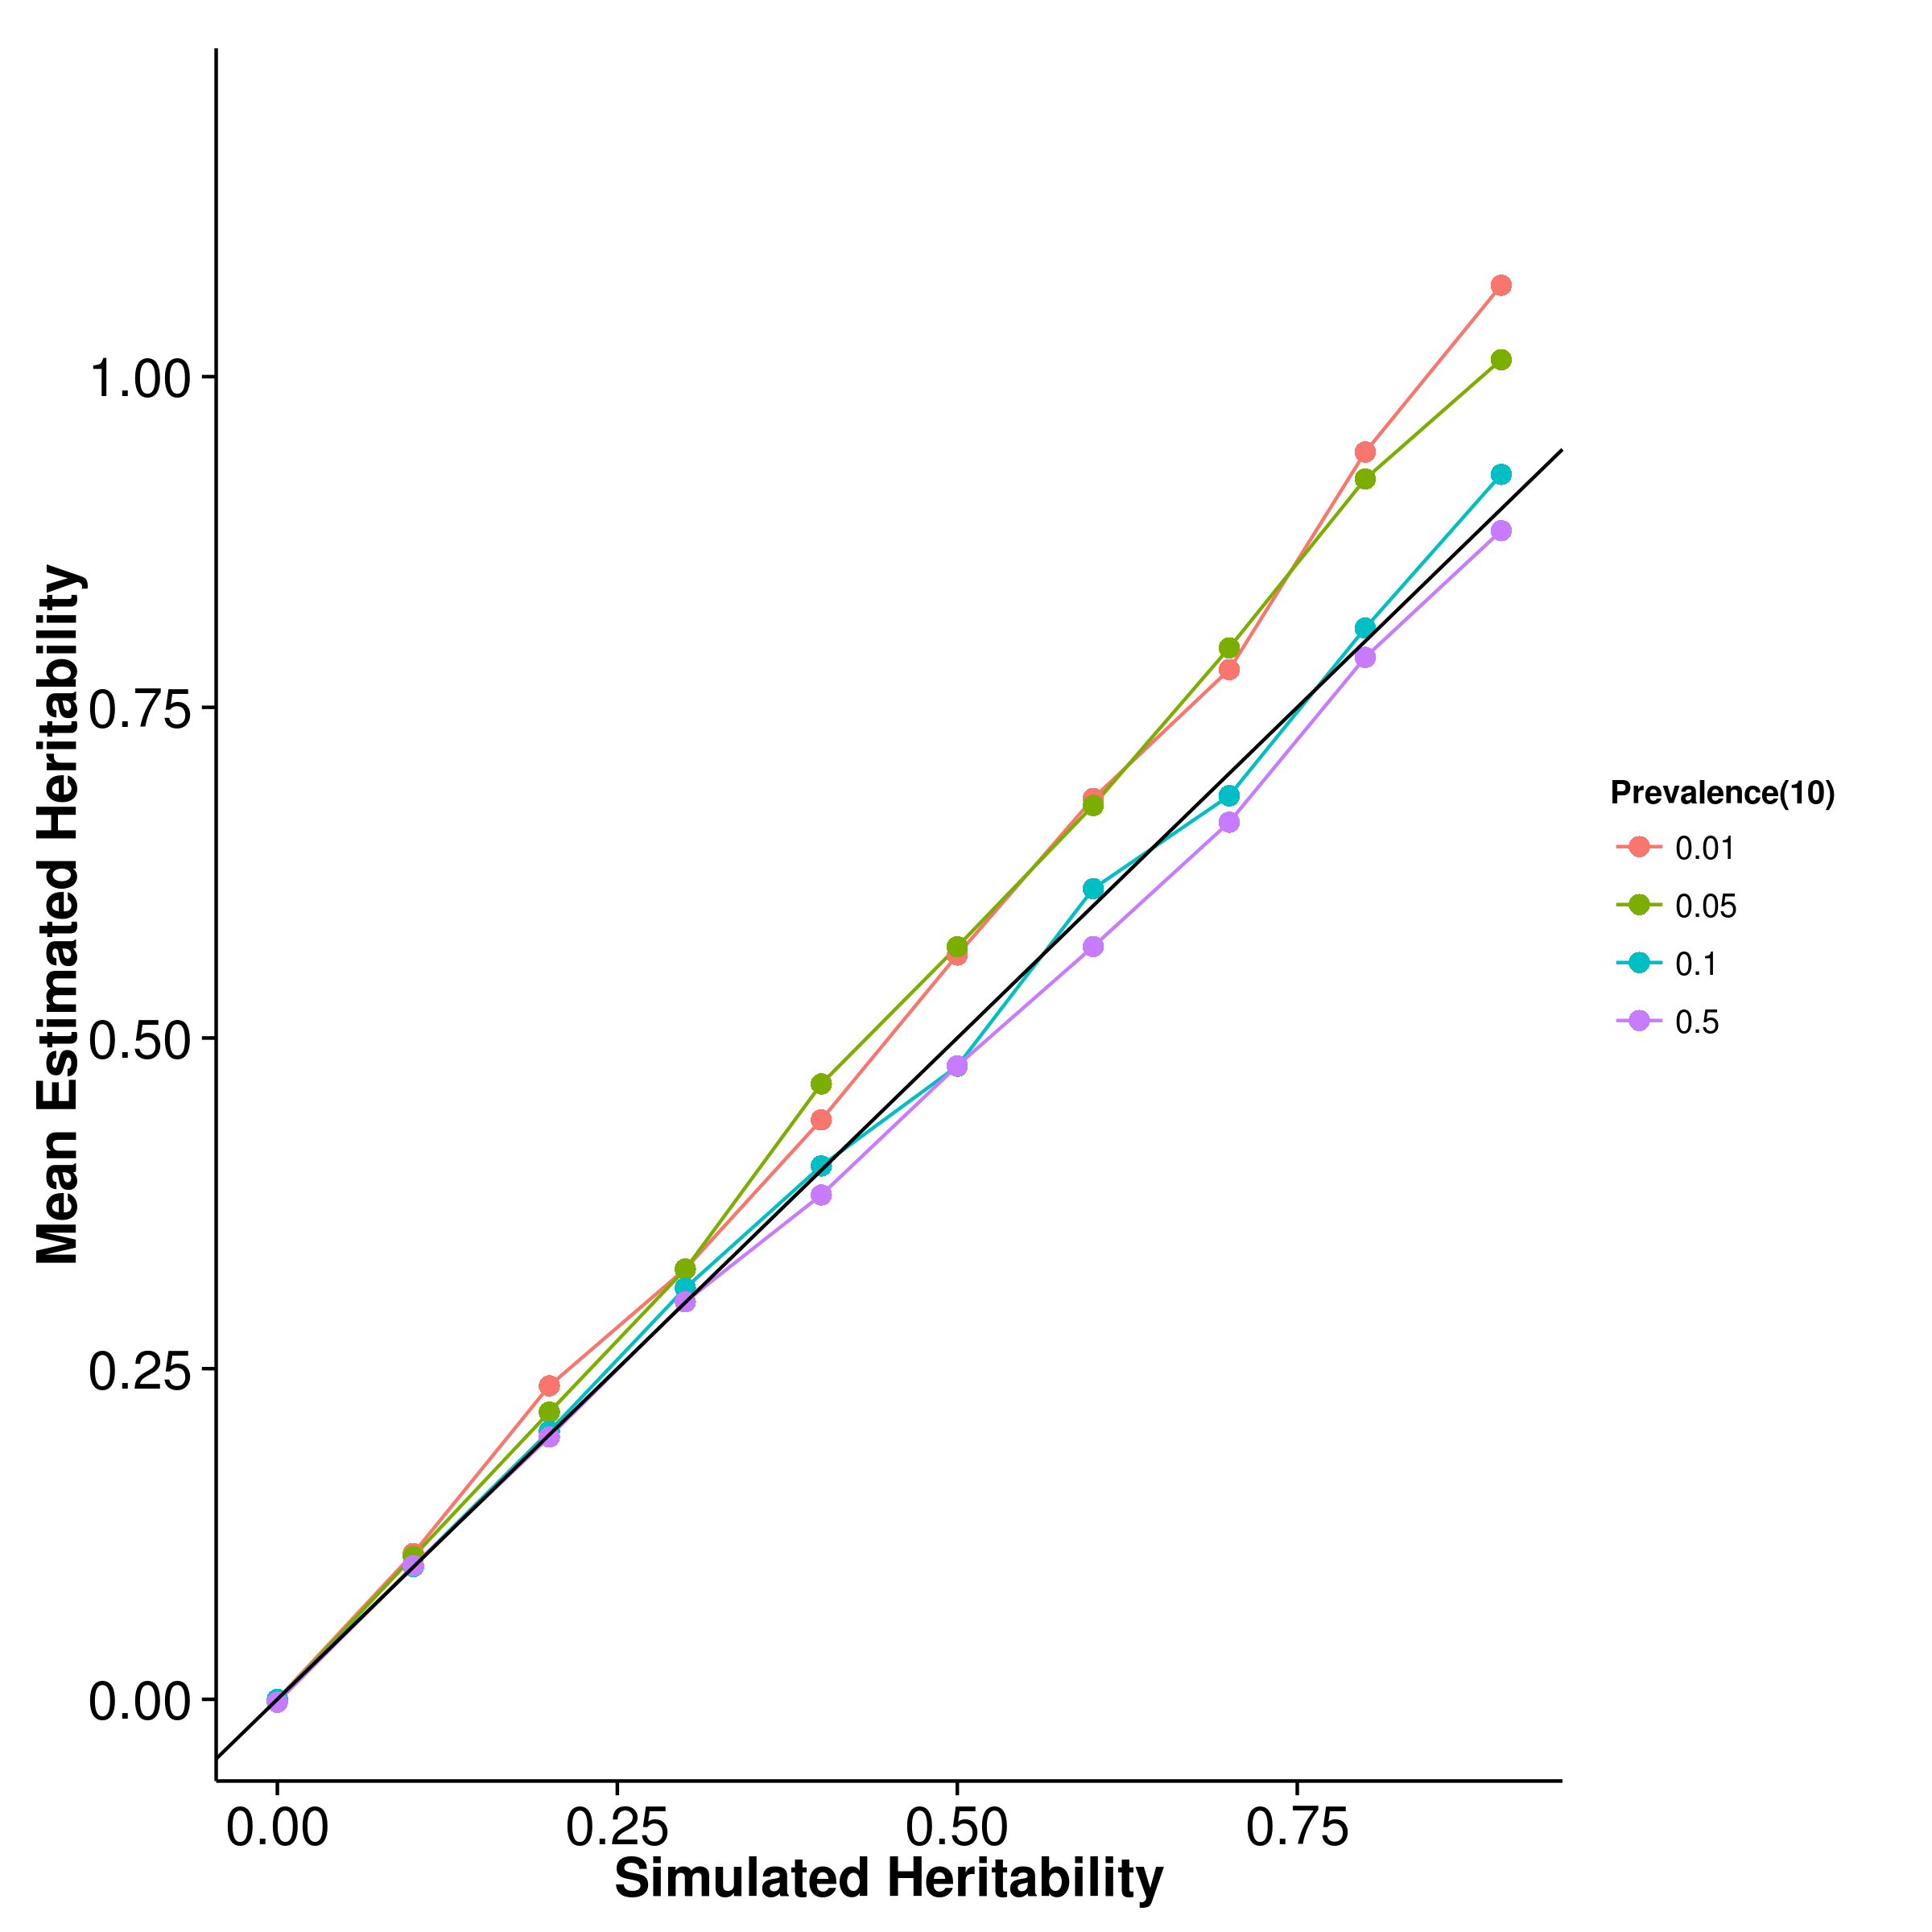
\includegraphics{figure/he_summary/cc_10c/shrek_CC_Rand_mean.png}}
				\label{fig:shrekCC10RandMean}
			}
			\subfloat[GCTA]{
				\scalebox{.4}{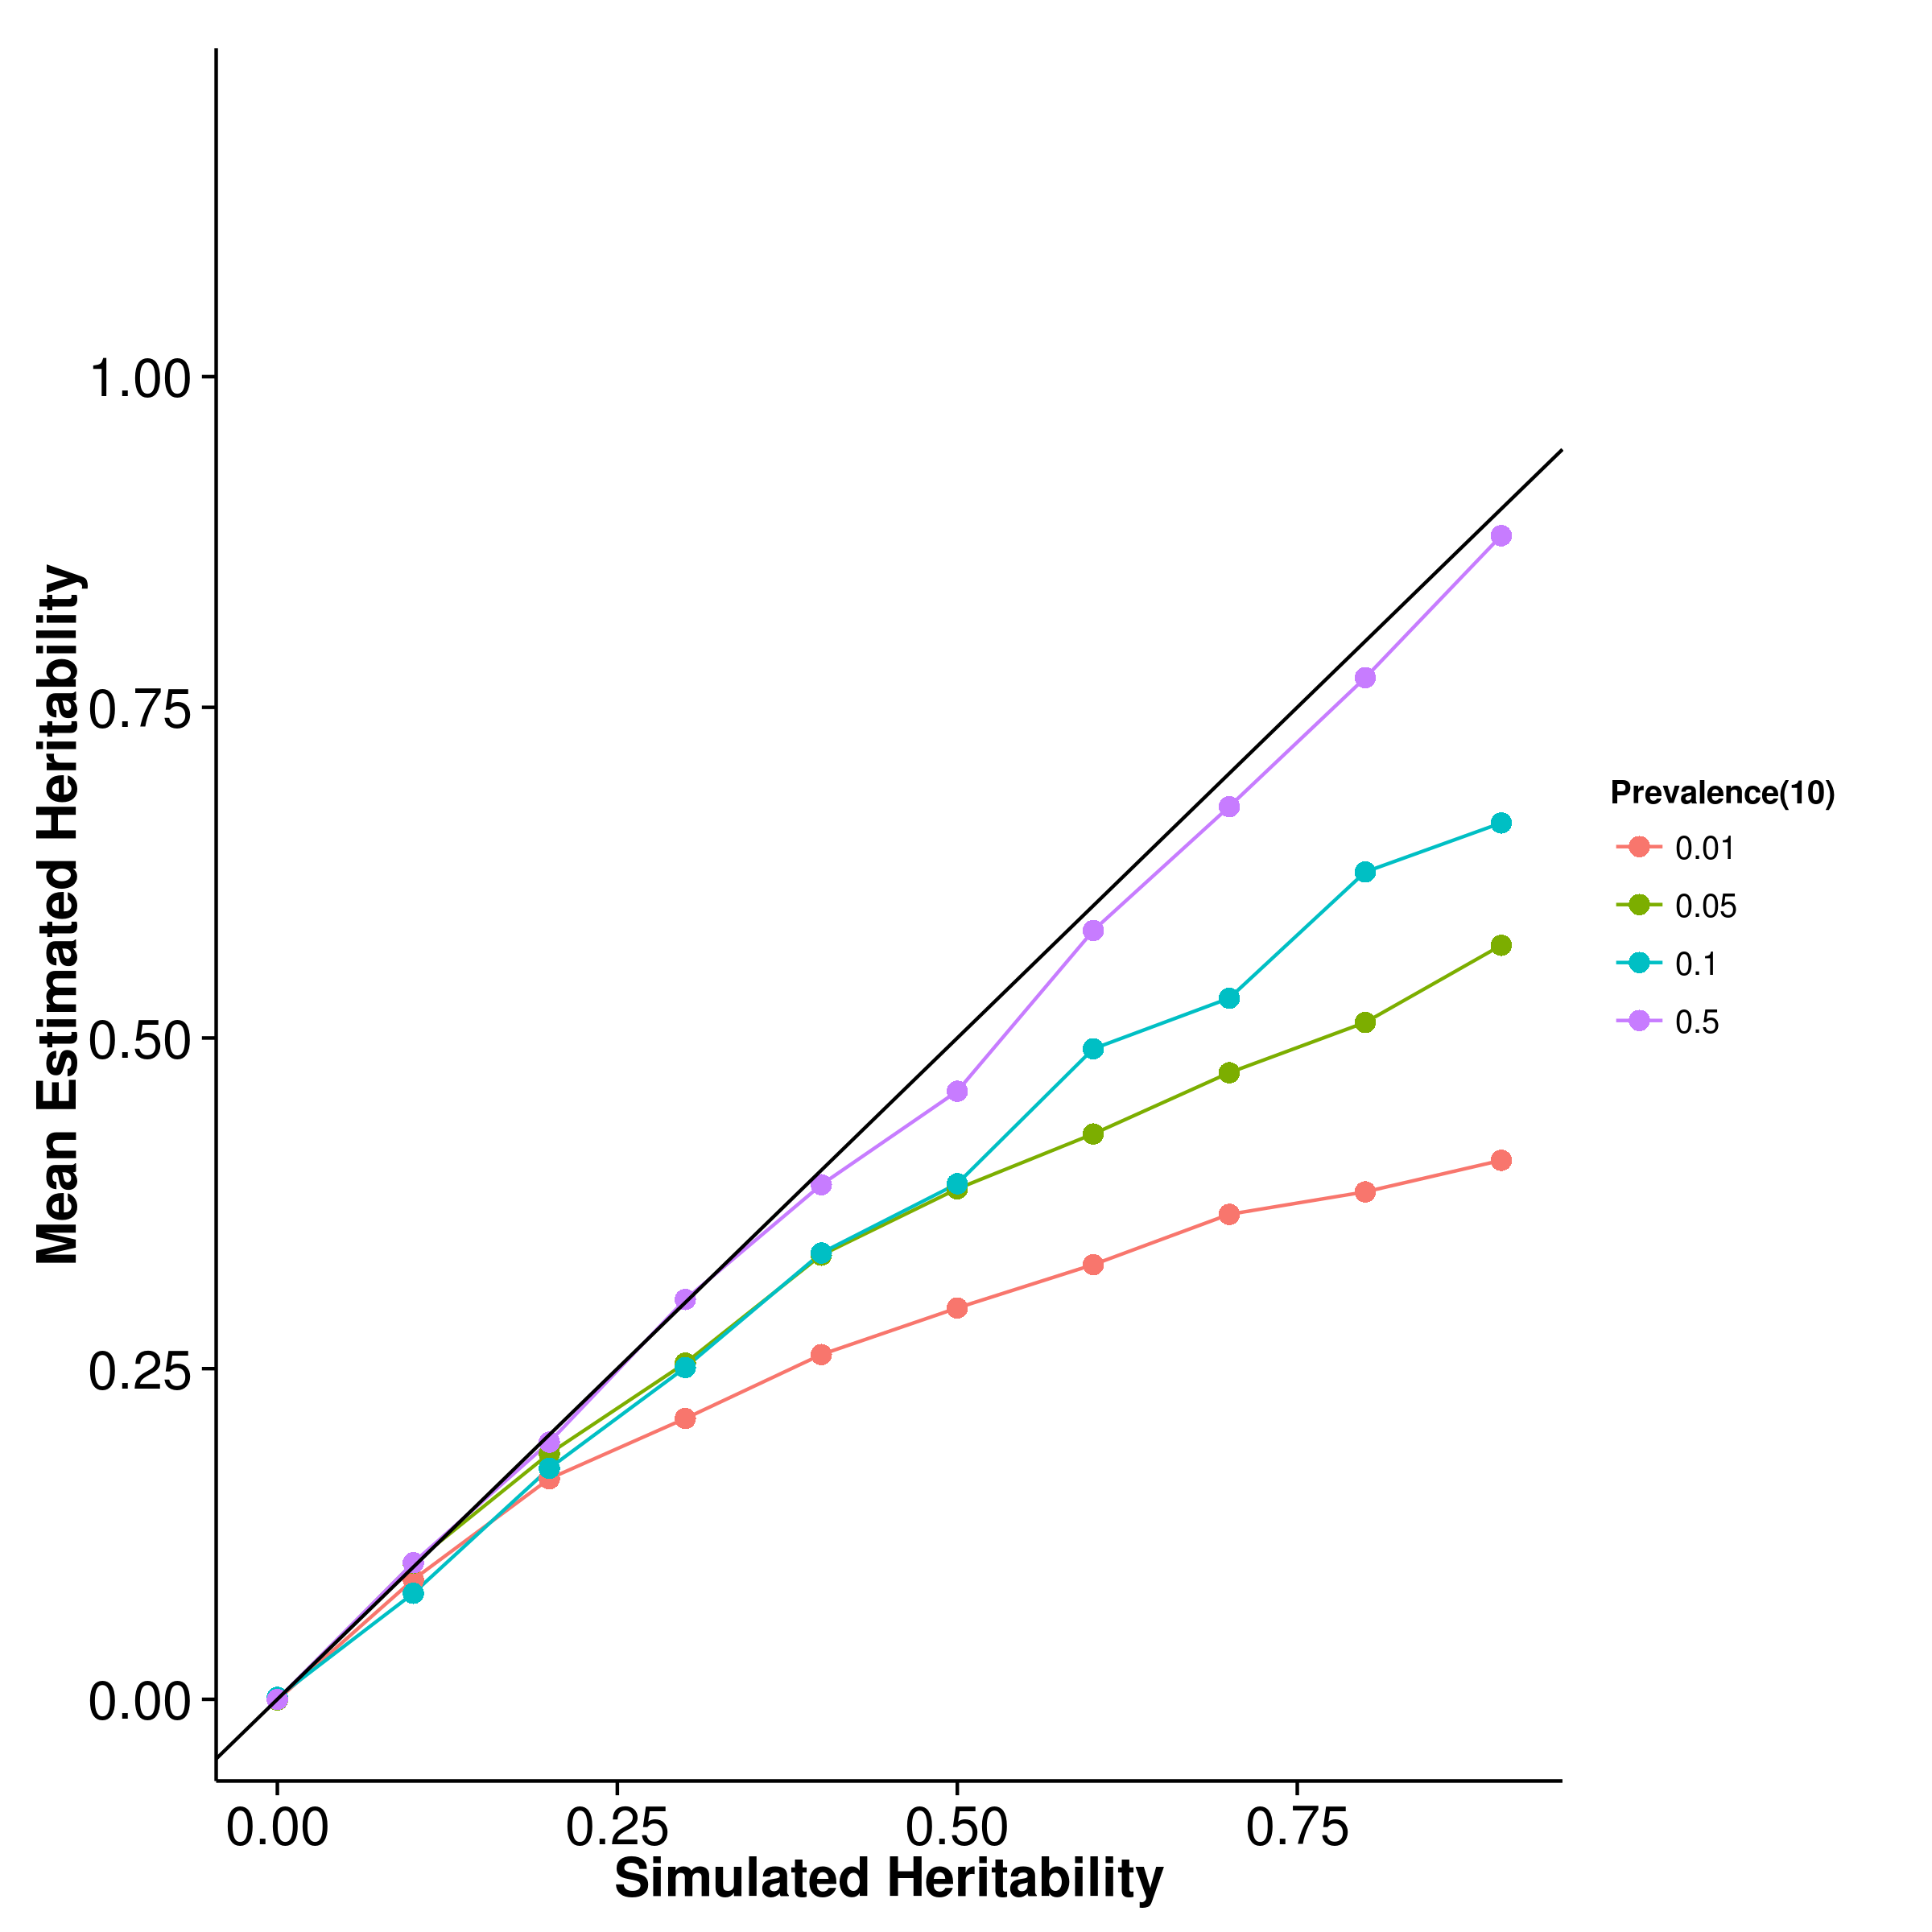
\includegraphics{figure/he_summary/cc_10c/gcta_CC_Rand_mean.png}}
				\label{fig:gctaCC10RandMean}
			}\\
			\subfloat[LDSC with fix intercept]{
				\scalebox{.4}{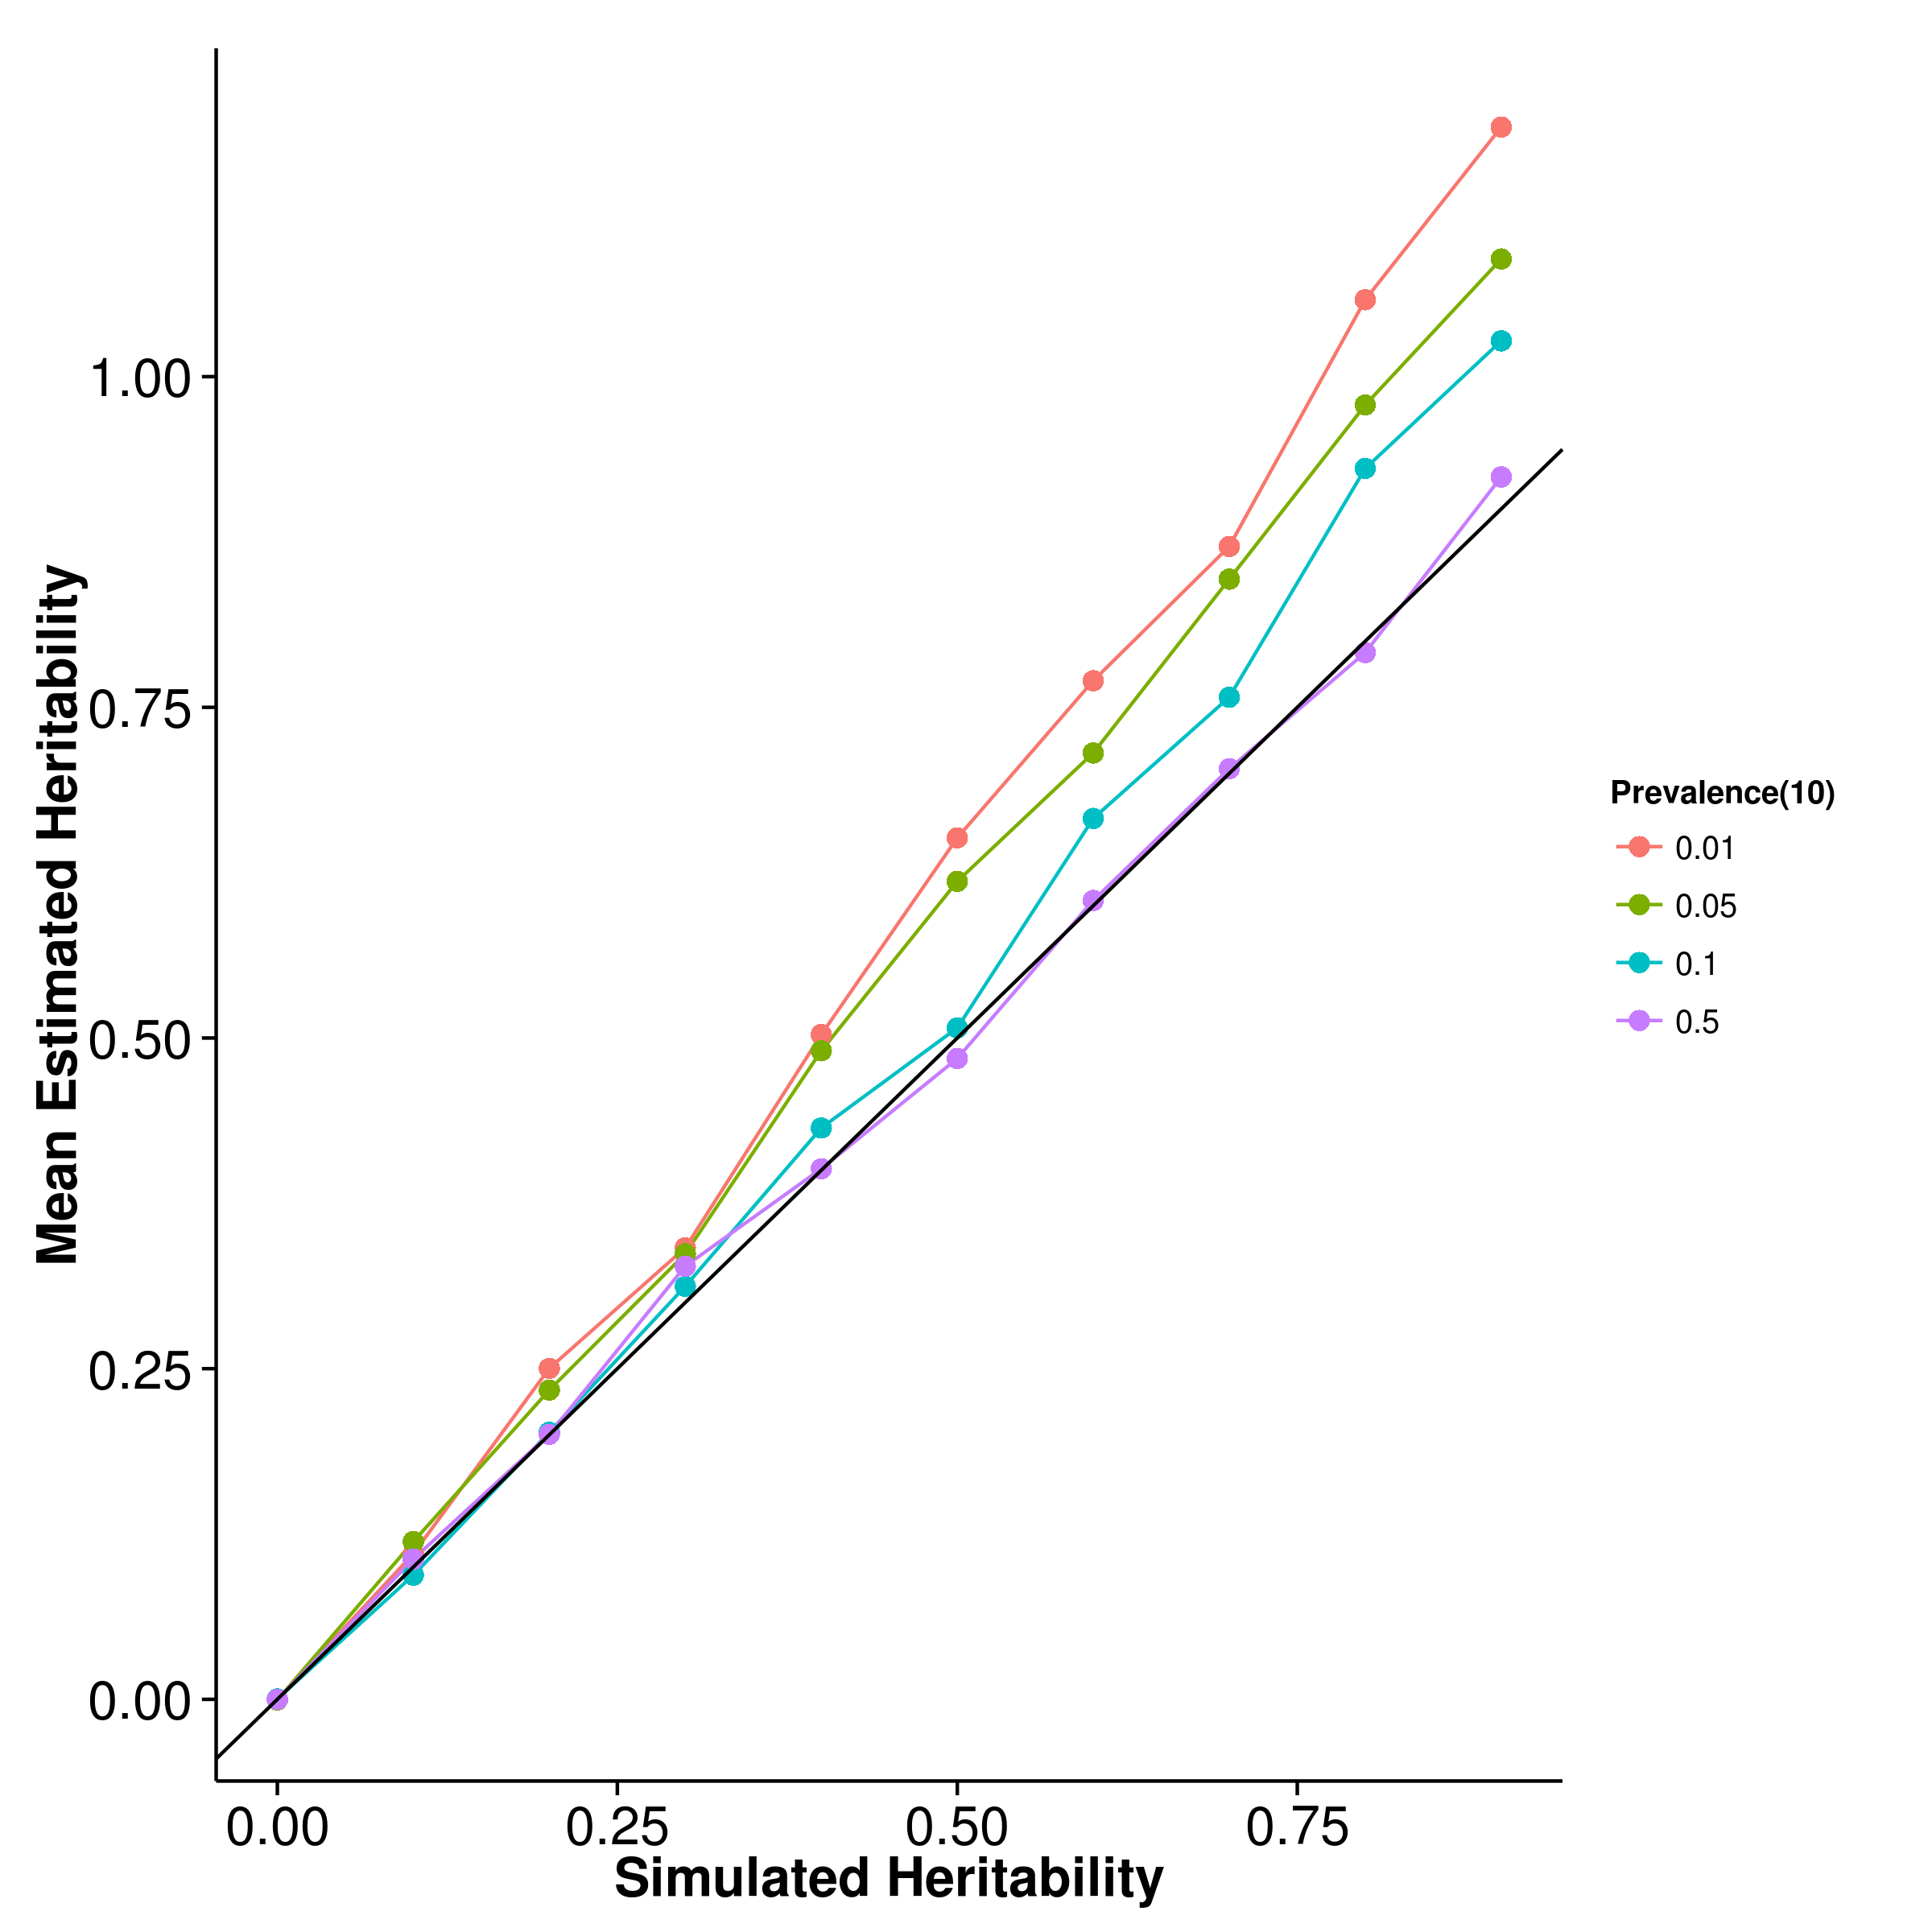
\includegraphics{figure/he_summary/cc_10c/ldsc_CC_Rand_mean.png}}
				\label{fig:ldscCC10RandMean}
			}
			\subfloat[LDSC with intercept estimation]{
				
				\scalebox{.4}{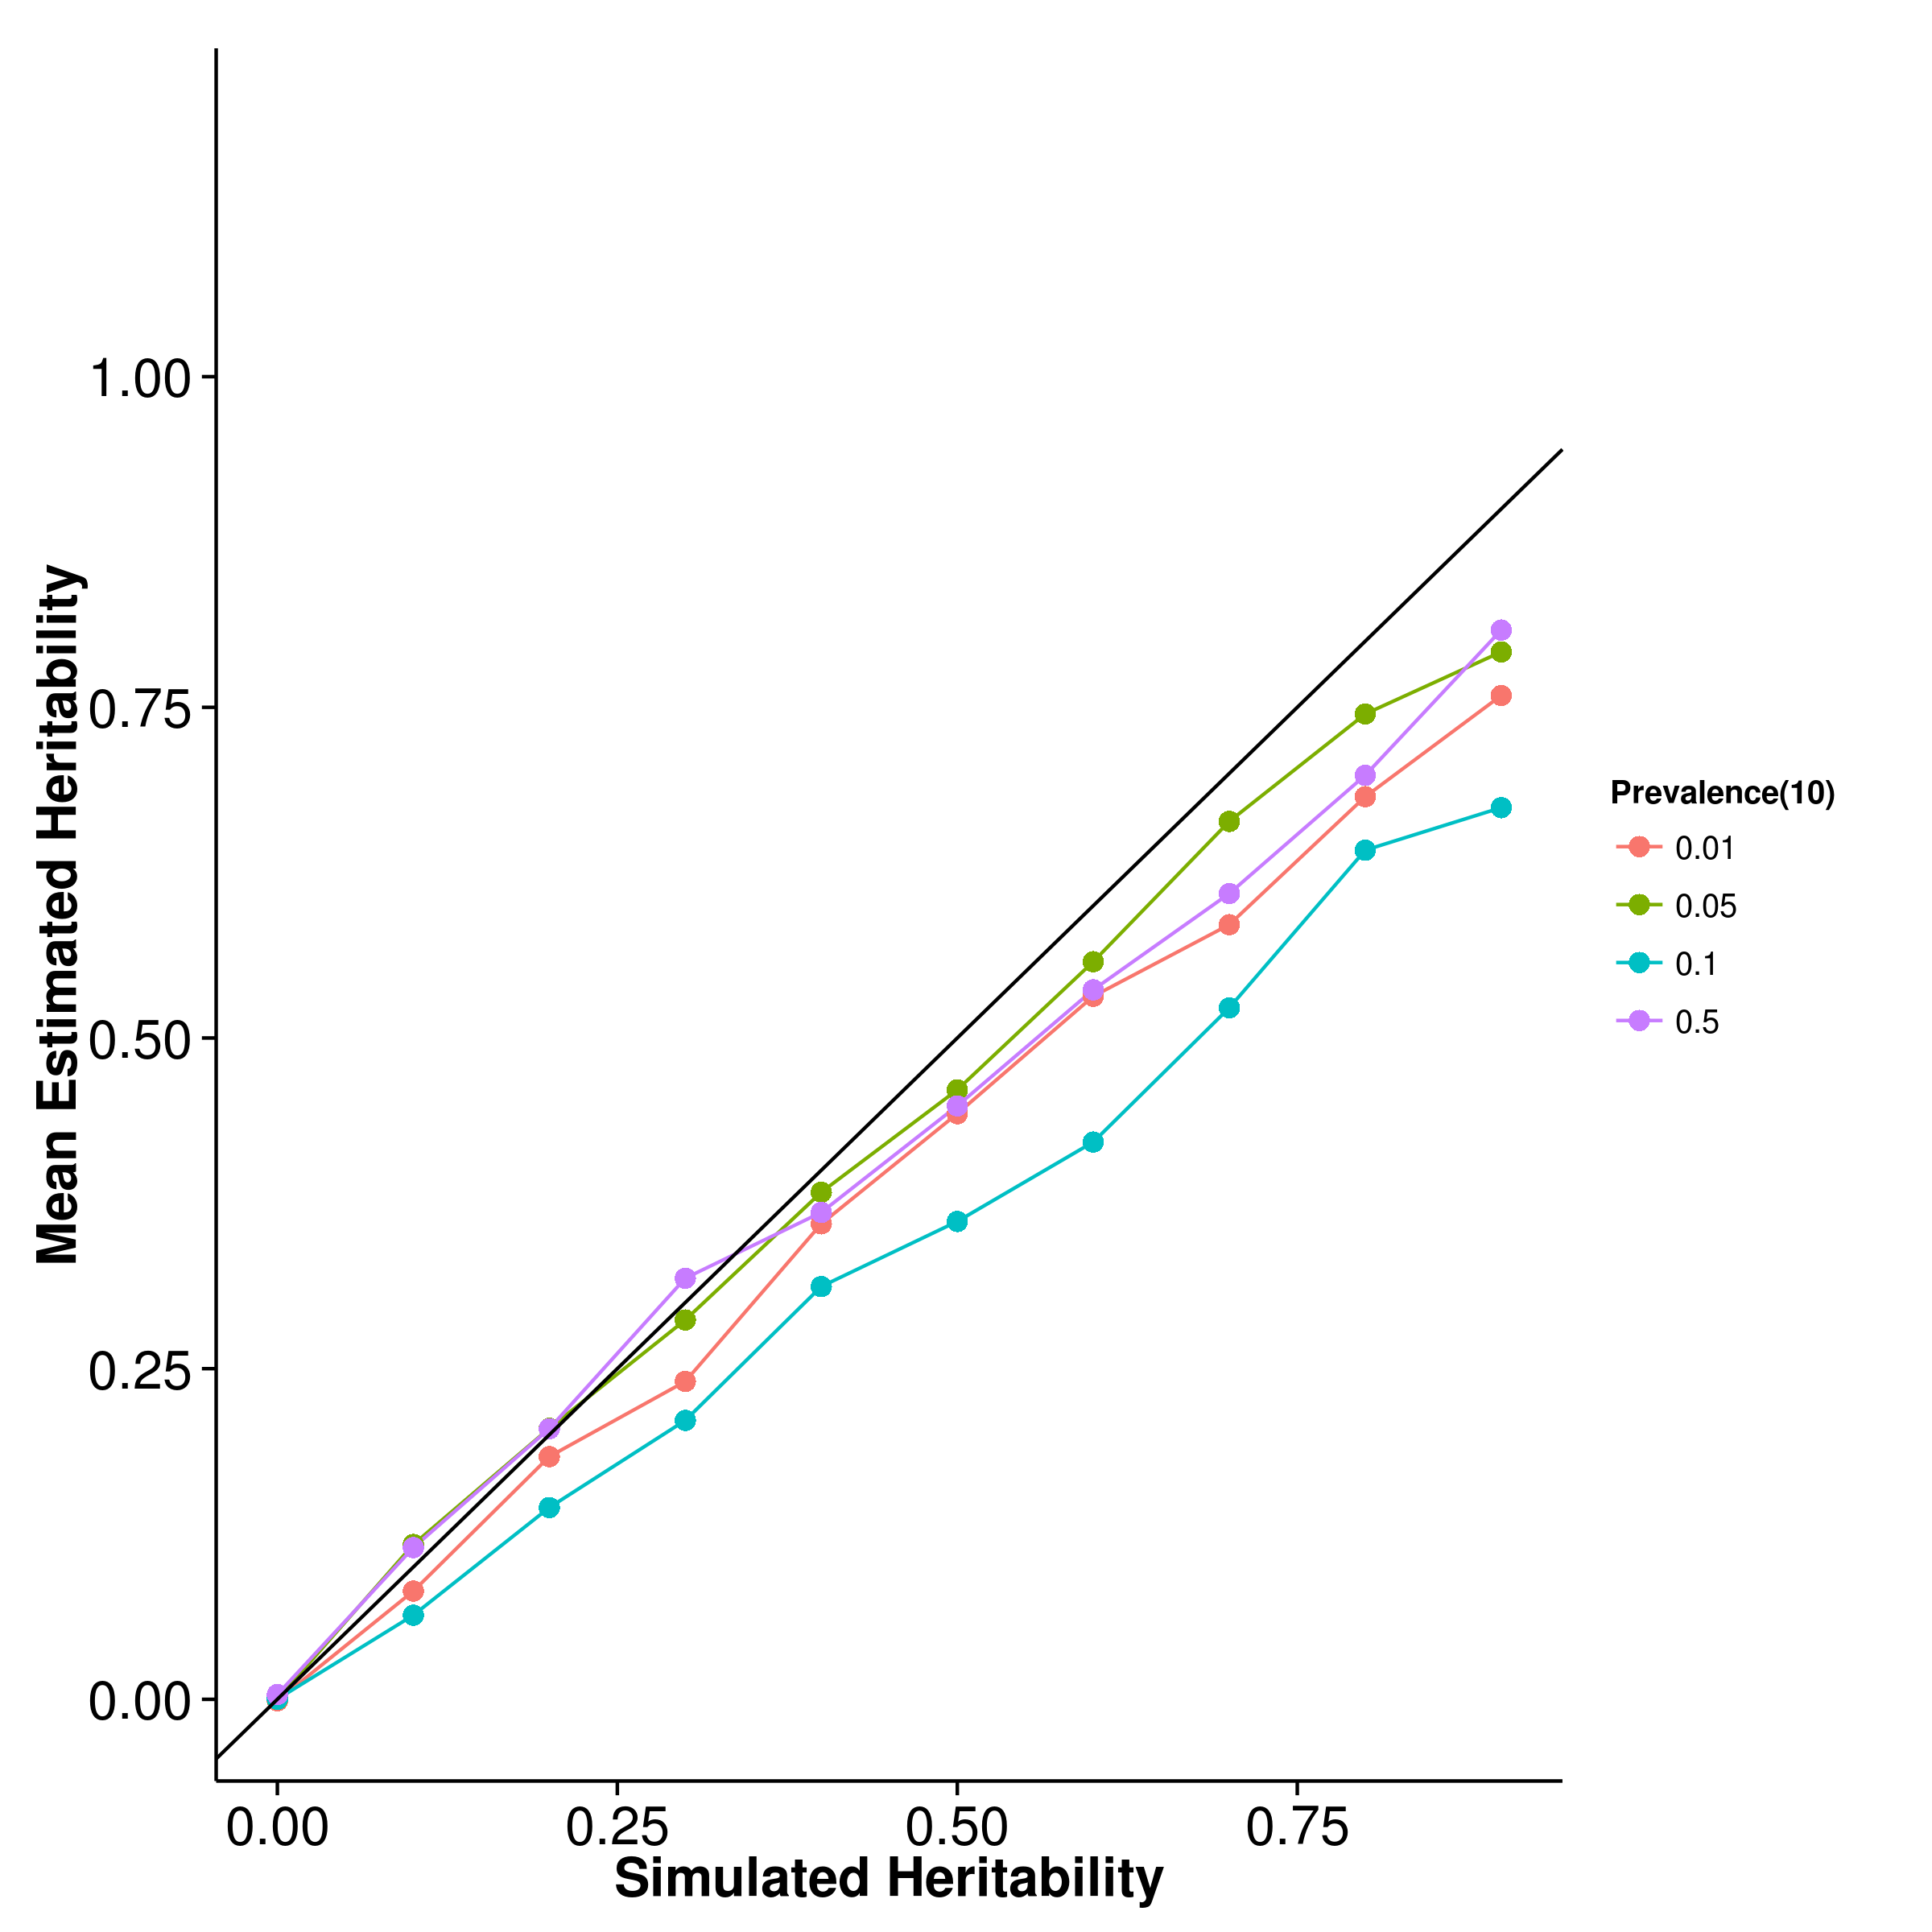
\includegraphics{figure/he_summary/cc_10c/ldscIn_CC_Rand_mean.png}}
				\label{fig:ldscInCC10RandMean}
			}
			\caption[Mean of Case Control Simulation Results (10 Causal)]
			{Mean of results from case control simulation with random effect size simulation with 10 causal \glspl{SNP}.
				The performance of \gls{gcta} was as suggested by \citet{Golan2014} where there was an underestimation as prevalence decreases.
				On the other hand, the upward bias of both \gls{ldsc} with fixed intercept and \gls{shrek} increases as the prevalence decreases whereas \gls{ldsc} with intercept estimation seems relatively robust to the change in prevalence.
				} 
			\label{fig:CC10RandMean}
		\end{figure}
		
		\begin{figure}
			\centering
			\subfloat[SHREK]{
				\scalebox{.4}{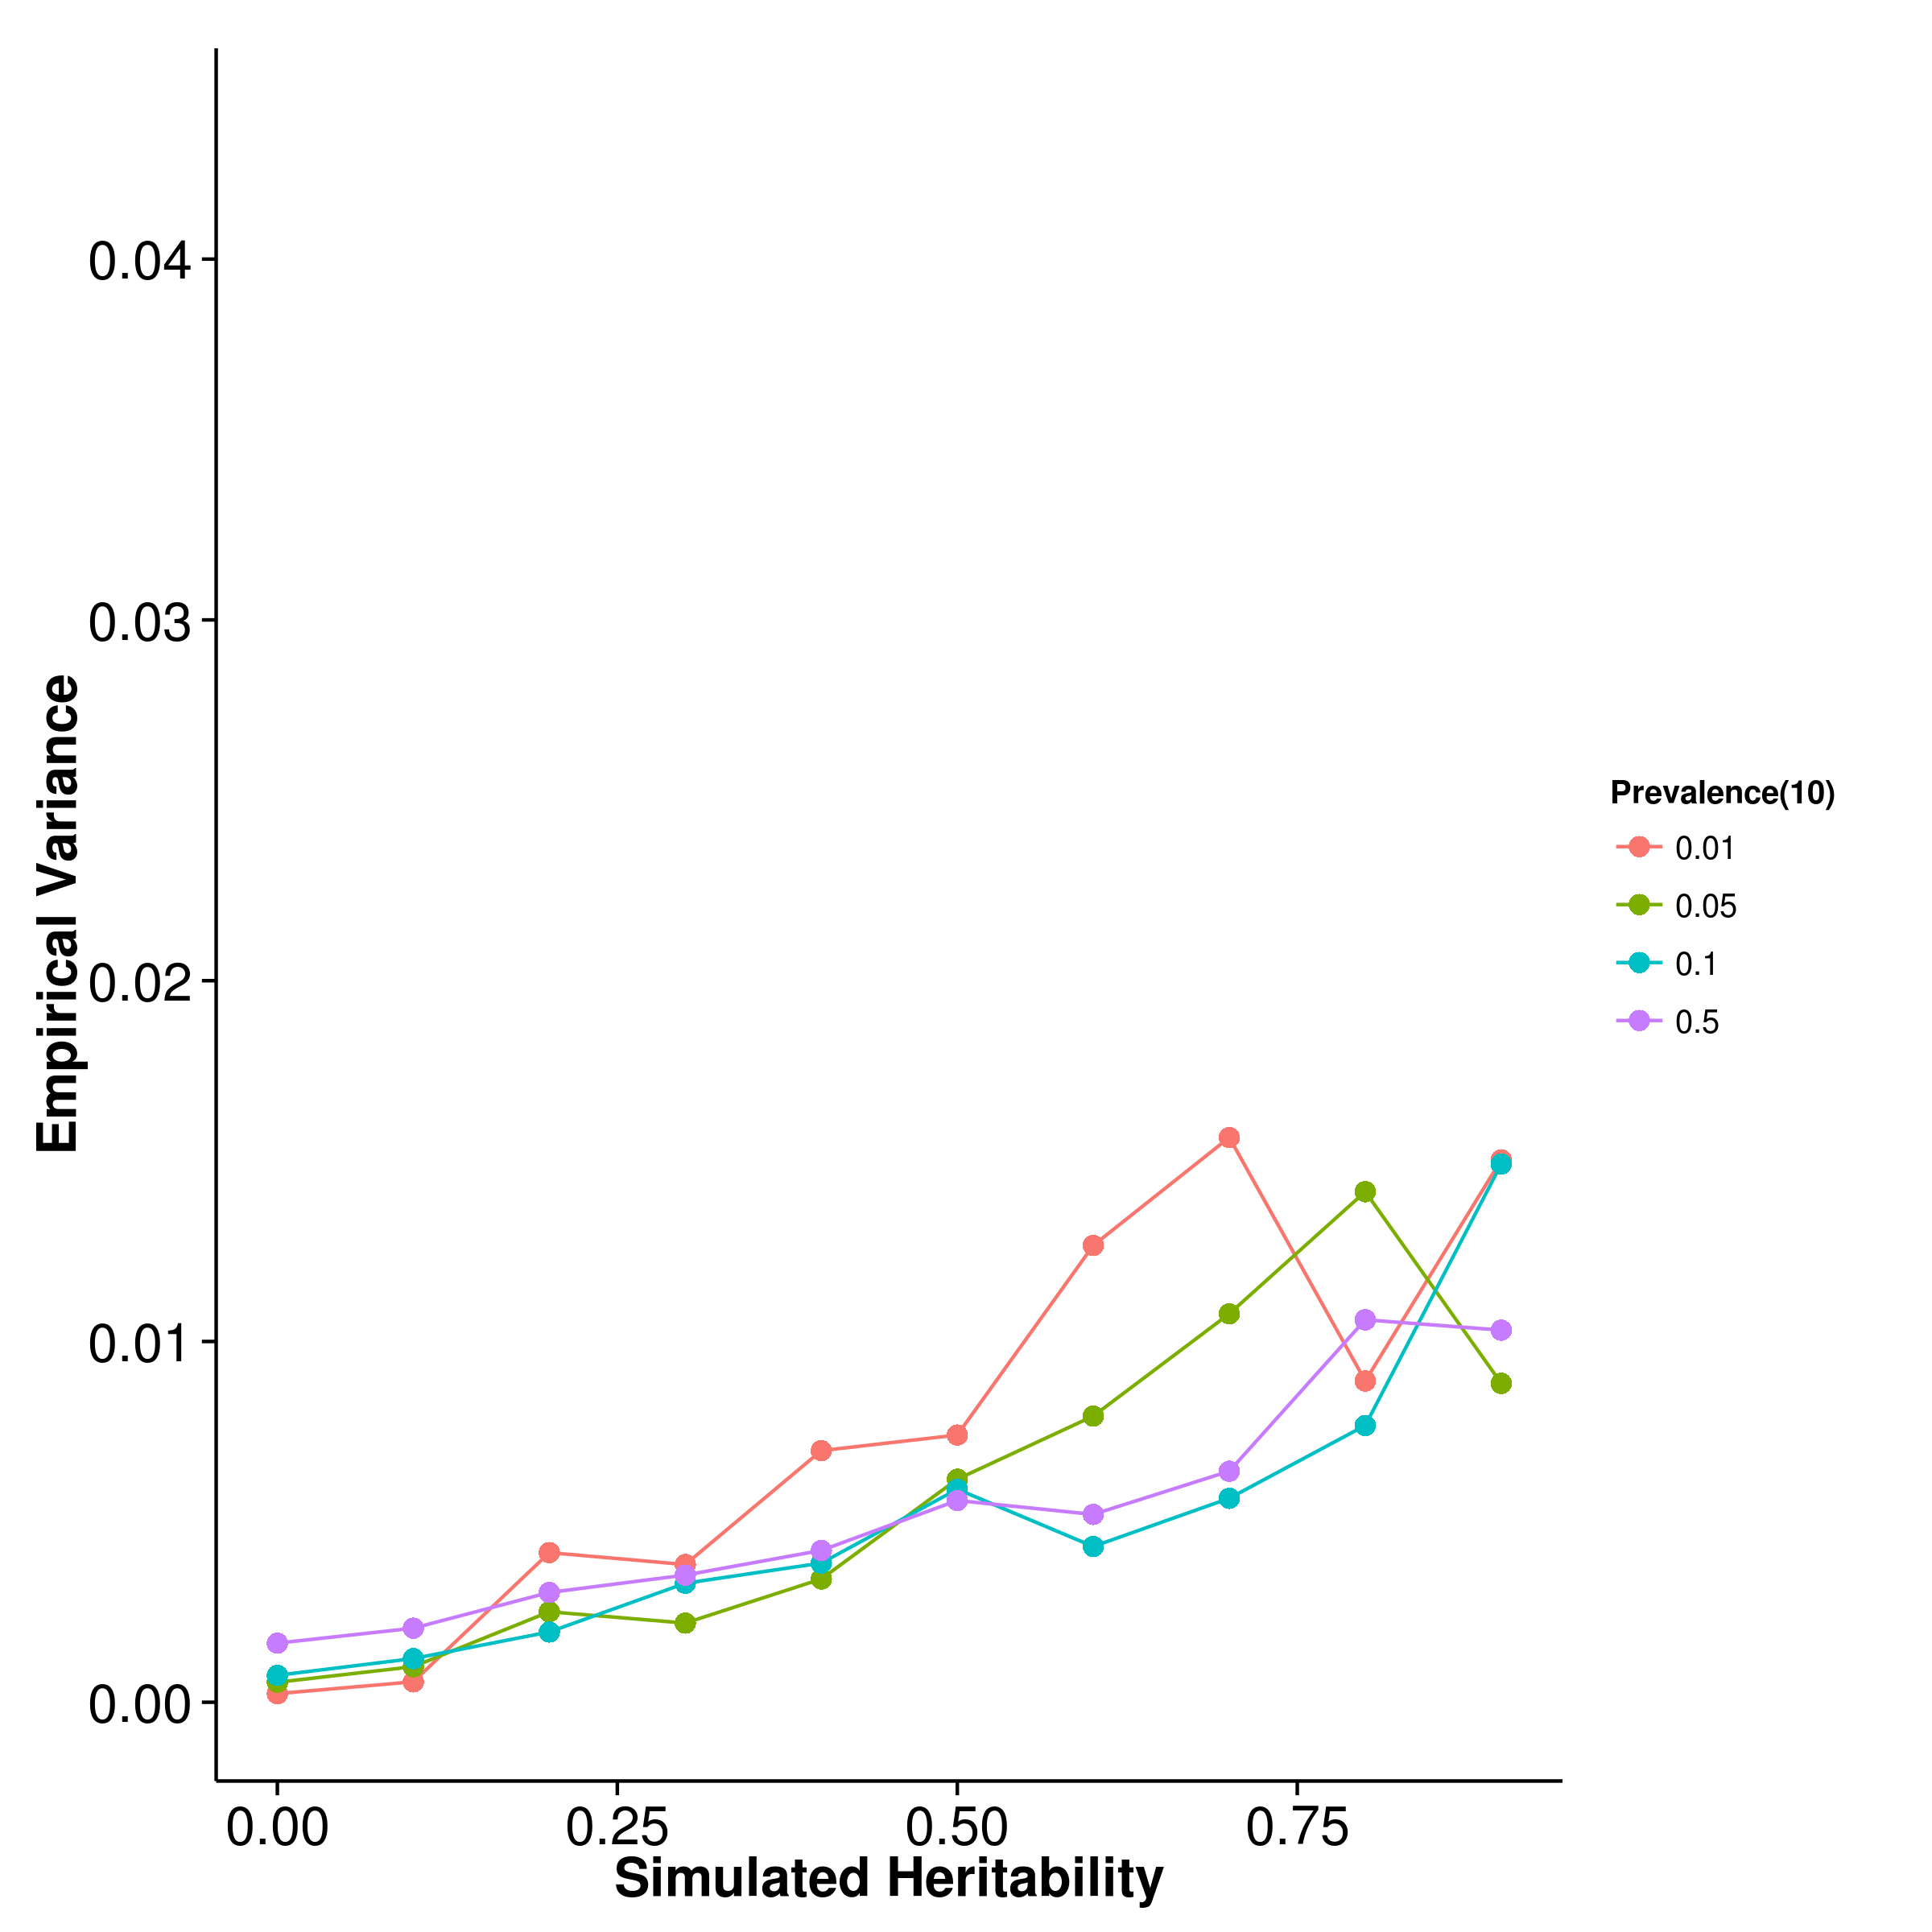
\includegraphics{figure/he_summary/cc_10c/shrek_CC_Rand_sd.png}}
				\label{fig:shrekCC10RandVar}
			}
			\subfloat[GCTA]{
				\scalebox{.4}{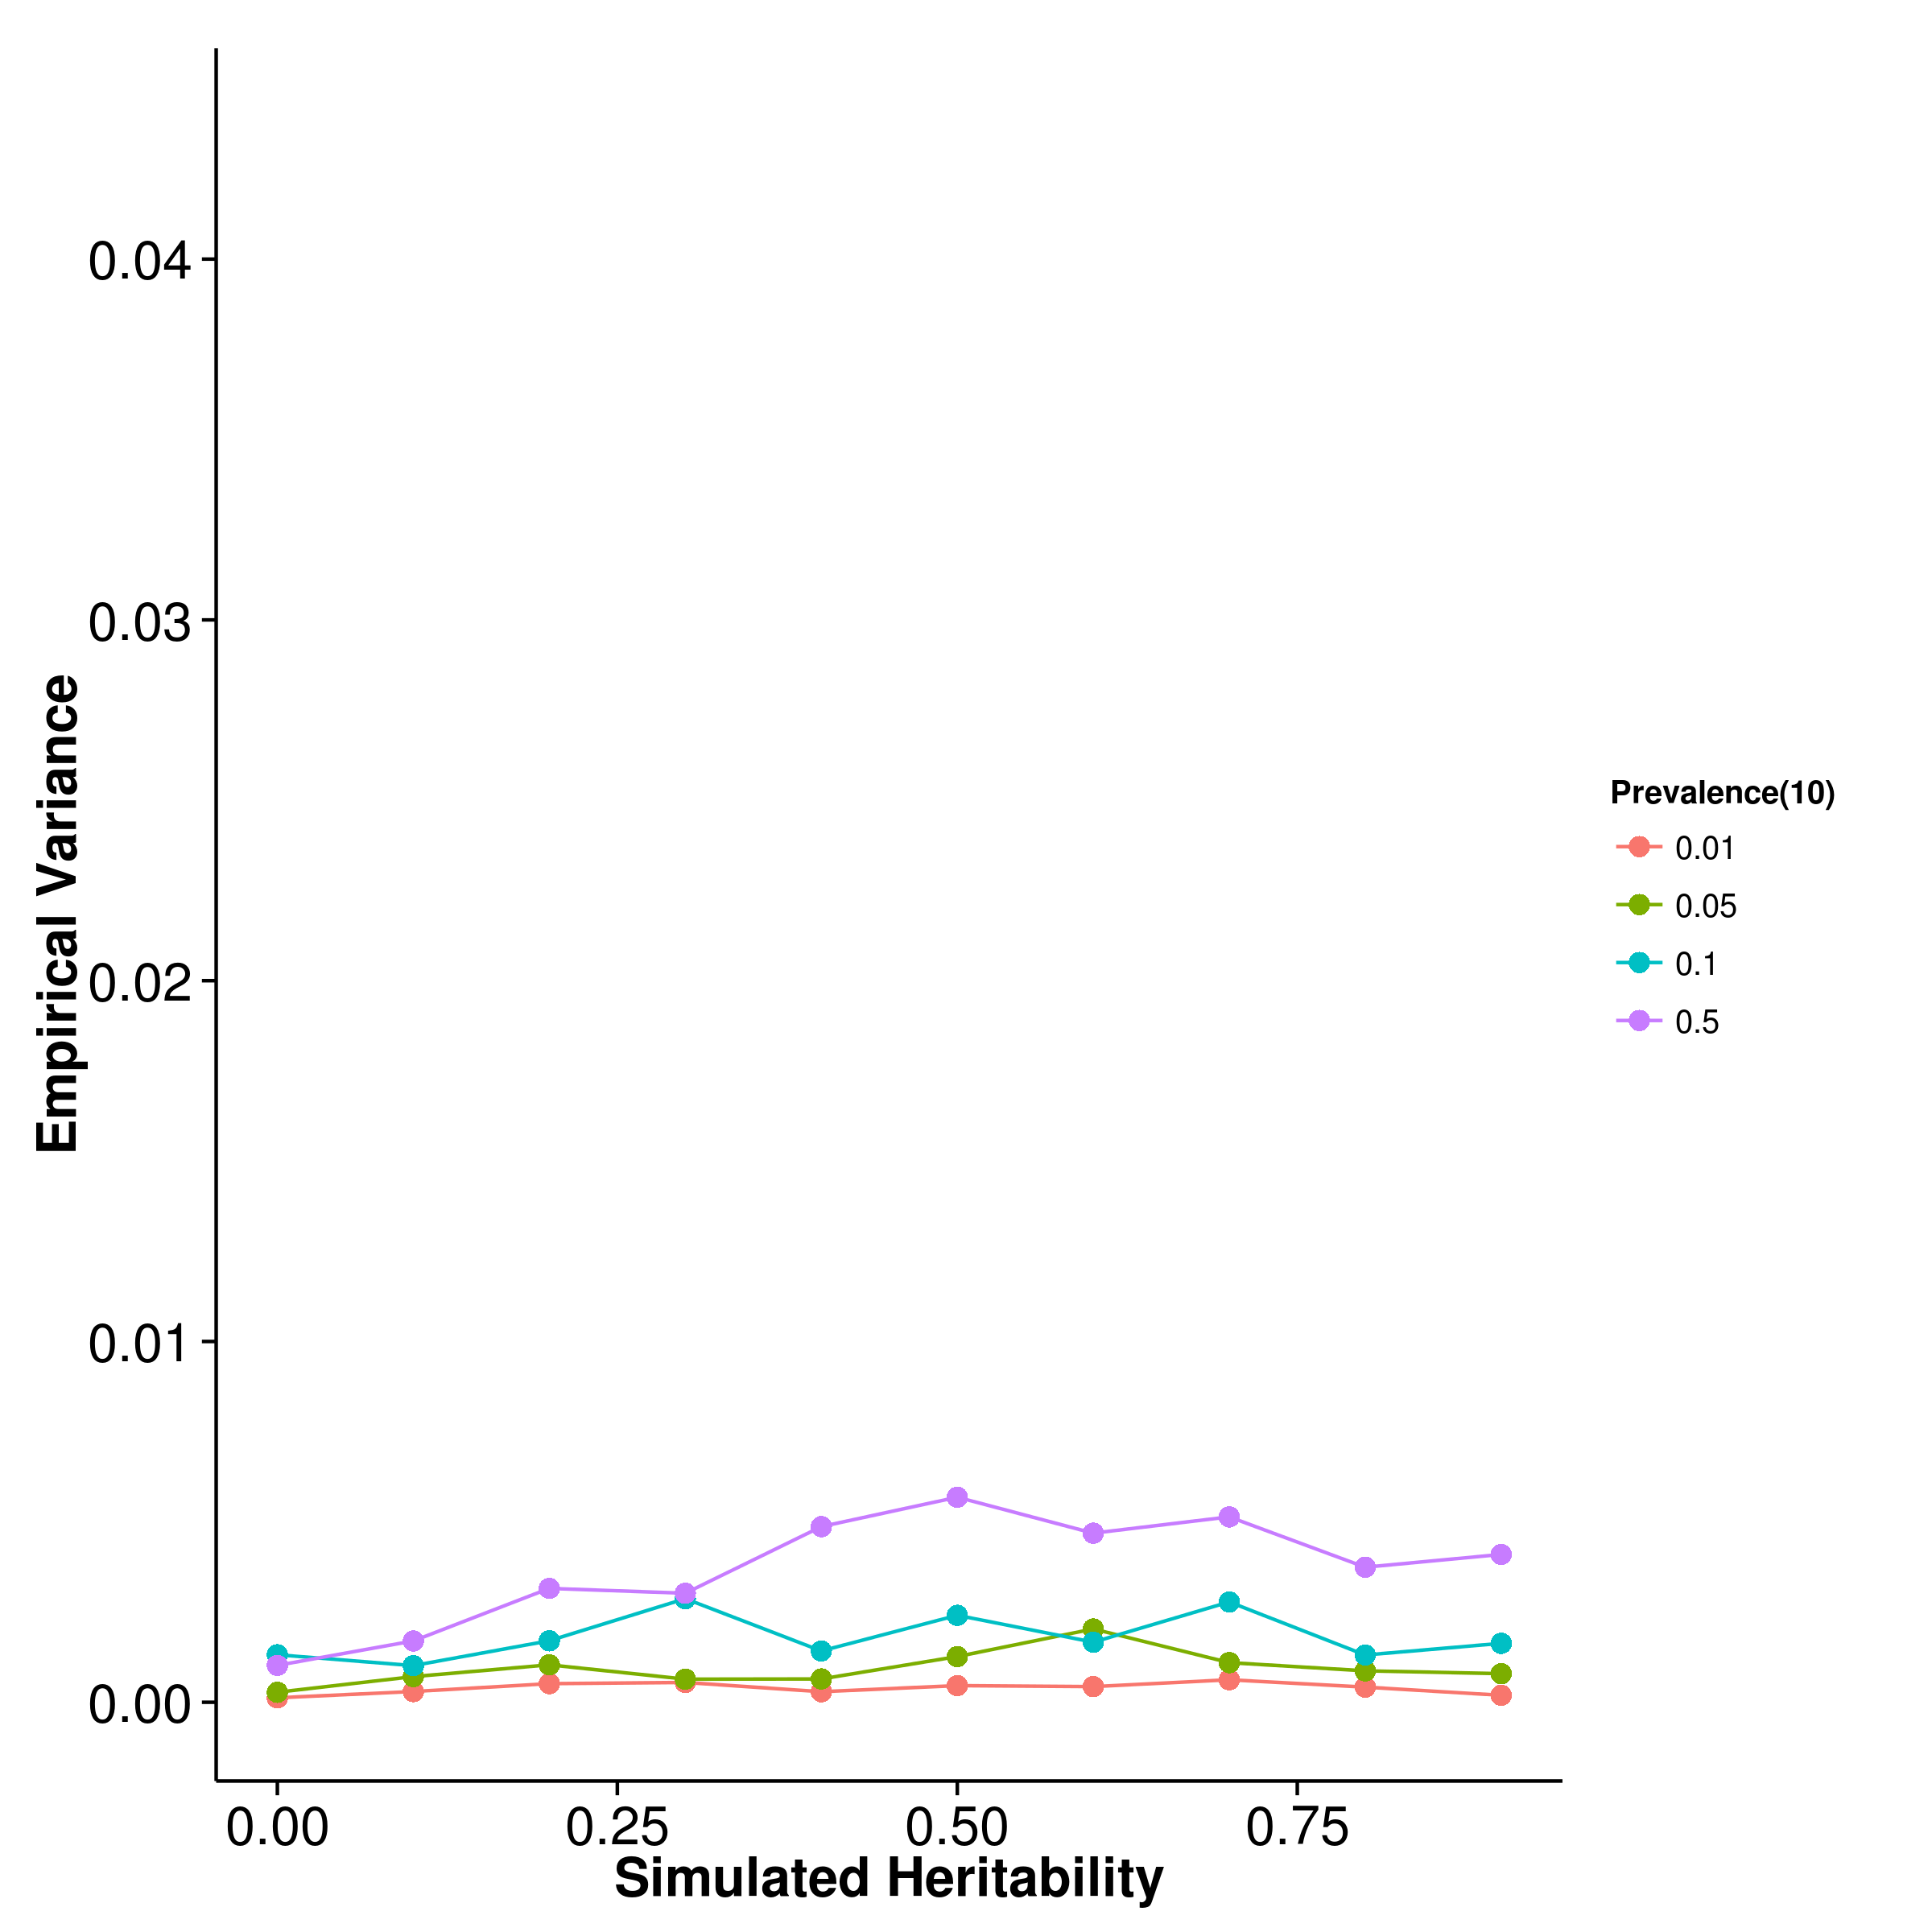
\includegraphics{figure/he_summary/cc_10c/gcta_CC_Rand_sd.png}}
				\label{fig:gctaCC10RandVar}
			}\\
			\subfloat[LDSC with fix intercept]{
				\scalebox{.4}{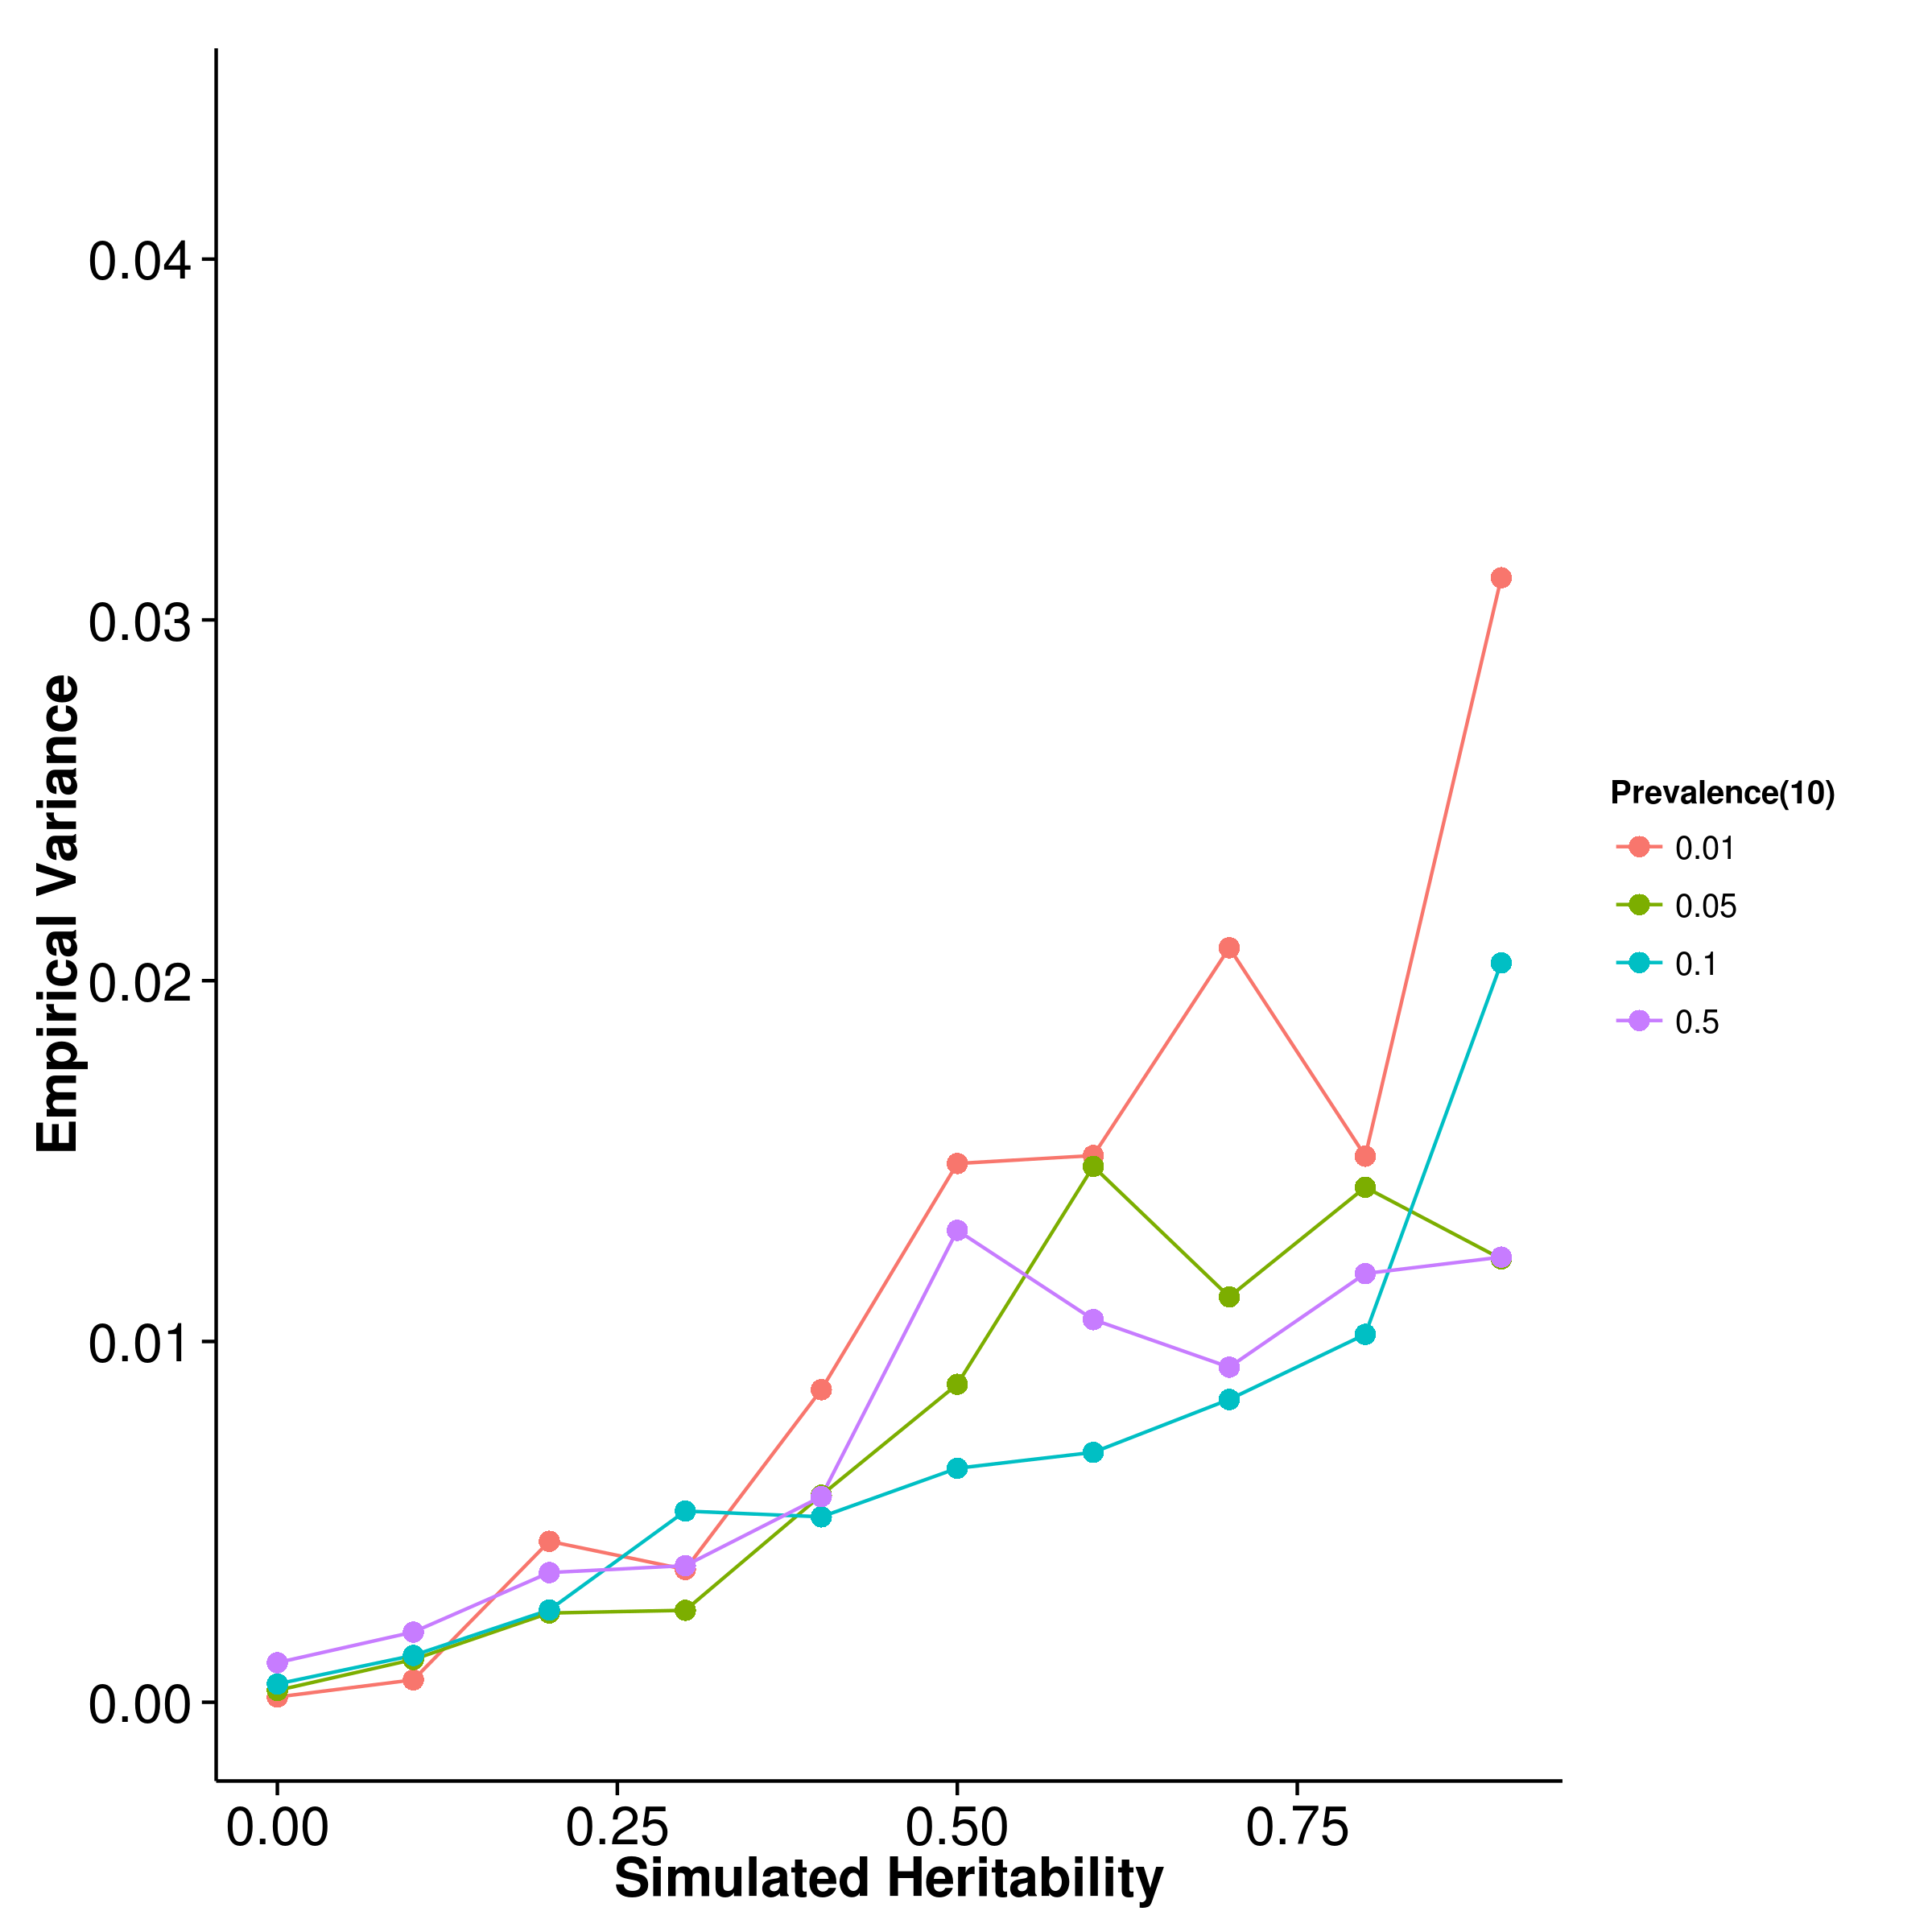
\includegraphics{figure/he_summary/cc_10c/ldsc_CC_Rand_sd.png}}
				\label{fig:ldscCC10RandVar}
			}
			\subfloat[LDSC with intercept estimation]{
				
				\scalebox{.4}{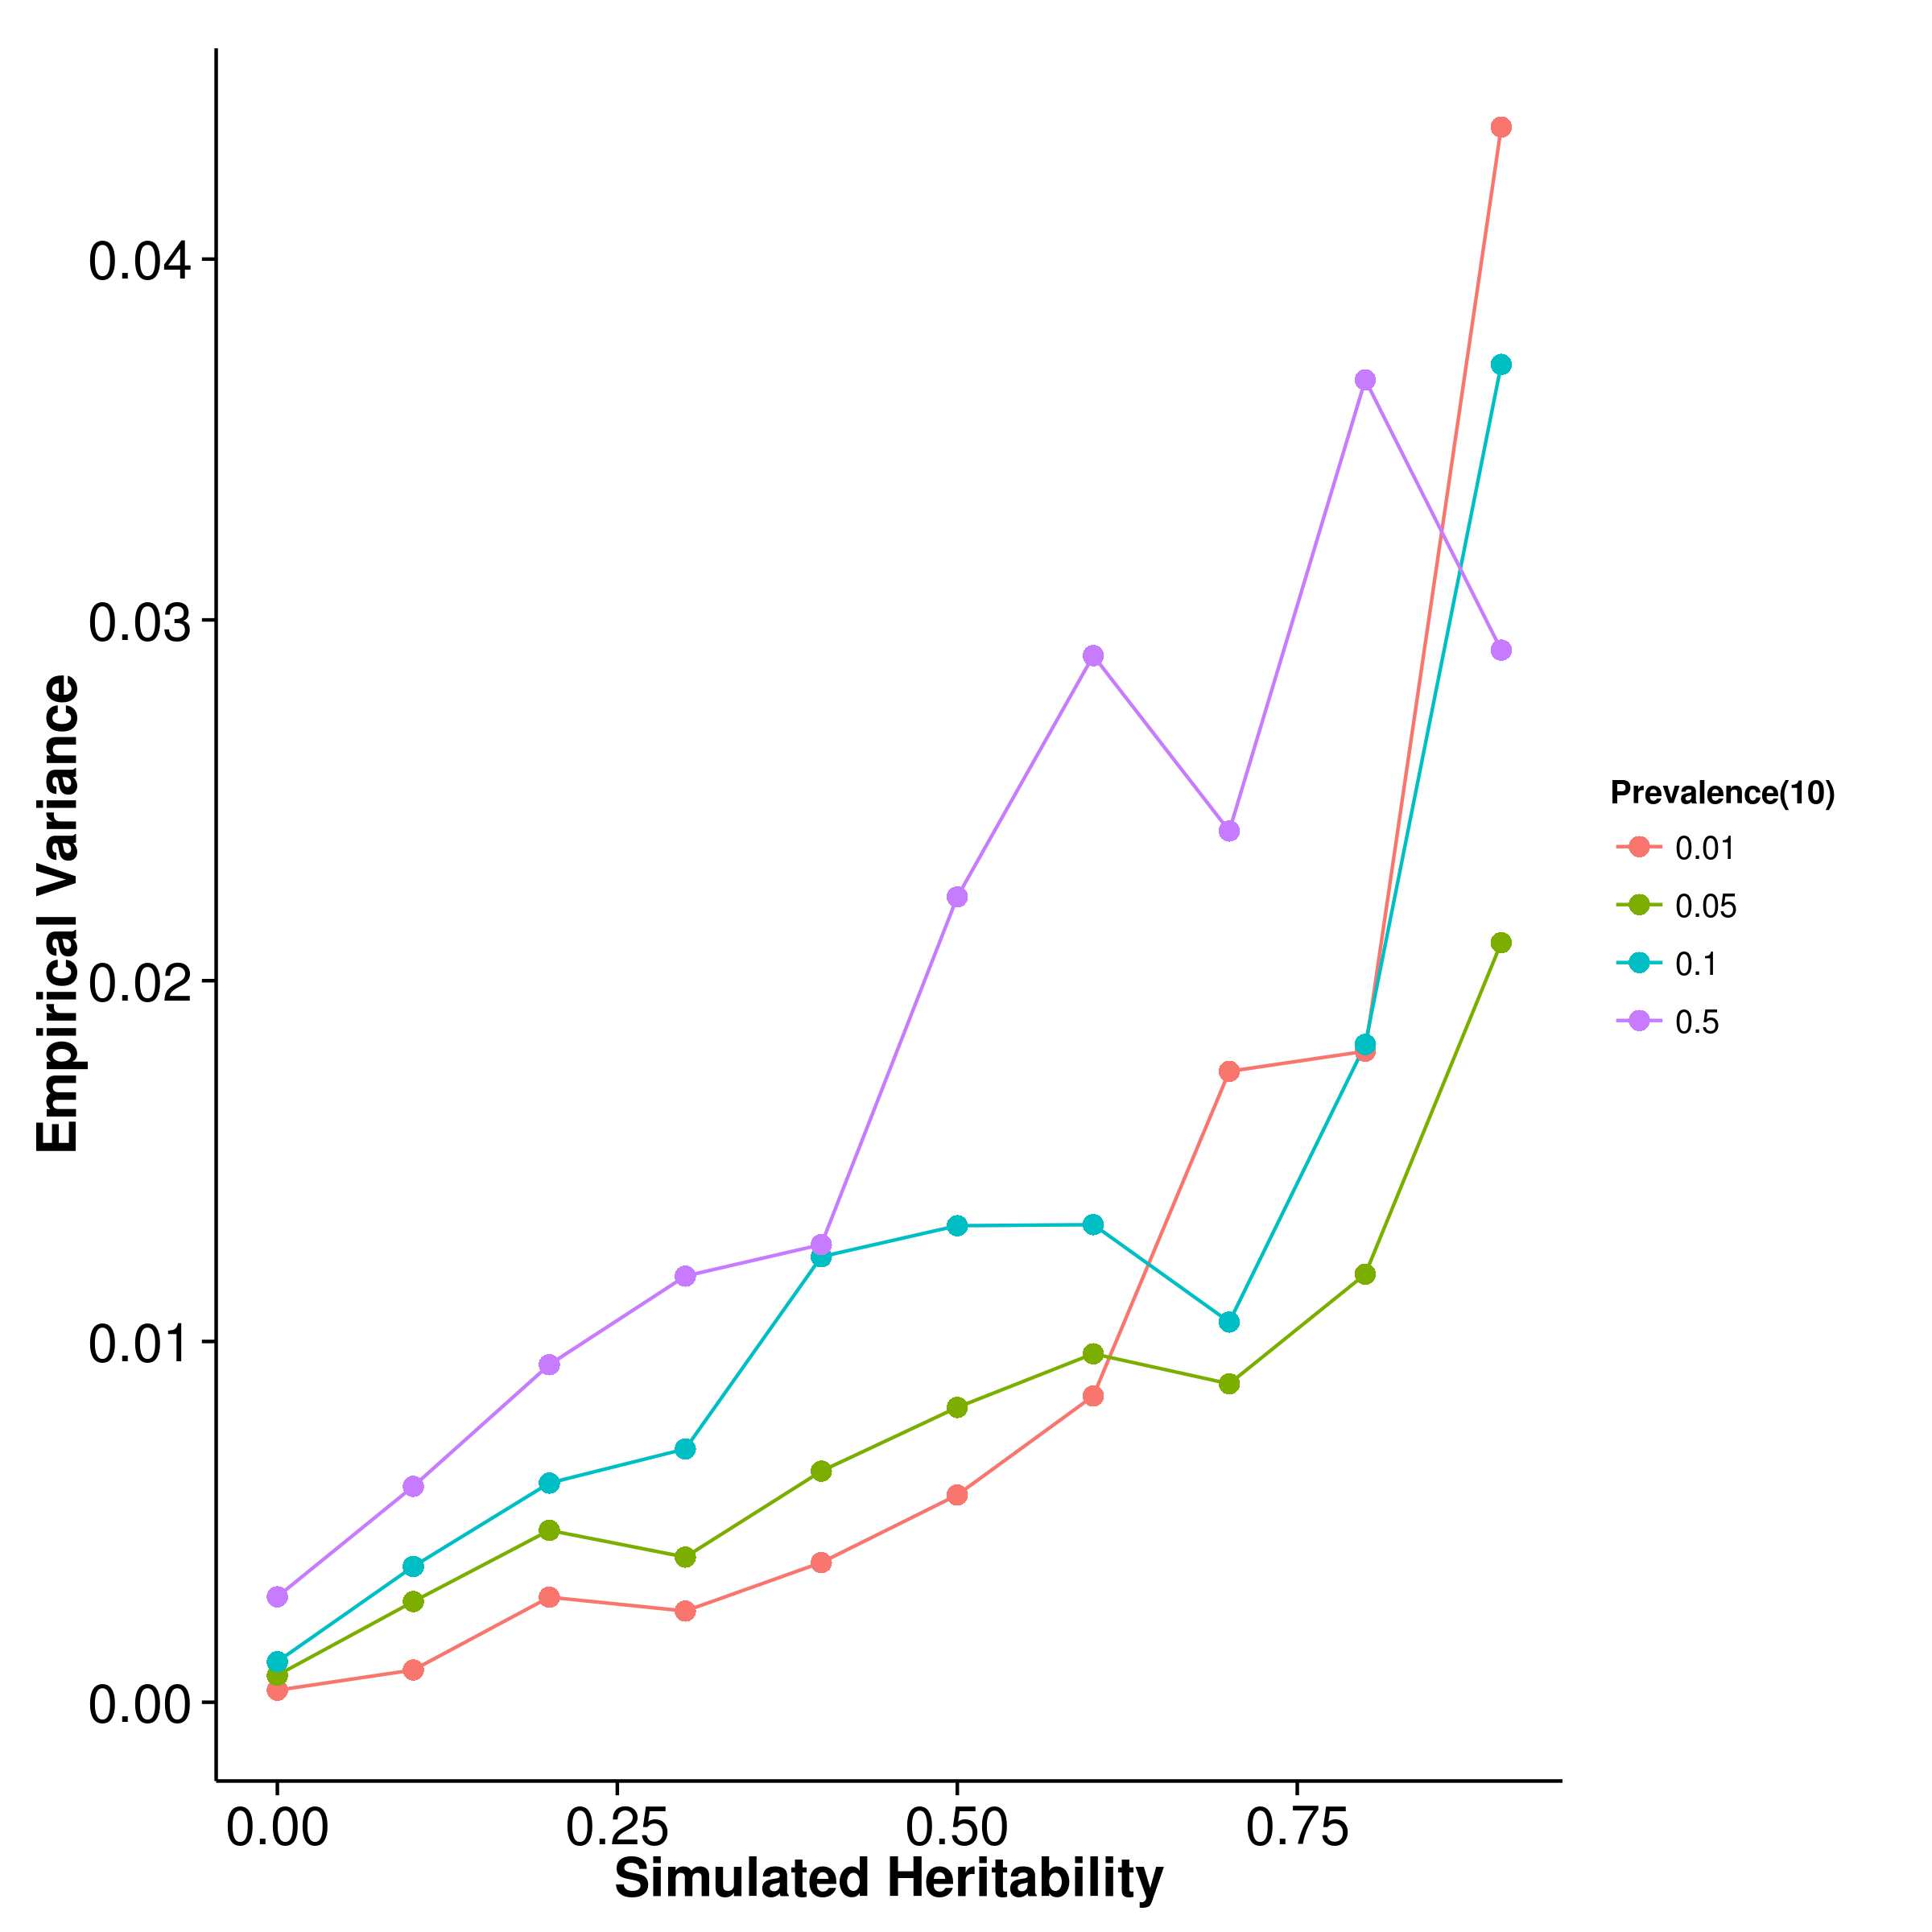
\includegraphics{figure/he_summary/cc_10c/ldscIn_CC_Rand_sd.png}}
				\label{fig:ldscInCC10RandVar}
			}
			\caption[Variance of Case Control Simulation Results (10 Causal)]
			{Variance of results from case control simulation with random effect size simulation with 10 causal \glspl{SNP}.
				There were no clear pattern as to how the prevalence affect the empirical variance of estimates from \gls{shrek} and \gls{ldsc}. 
				For \gls{gcta}, it seems like a larger prevalence tends to result in a larger empirical variance. 
				Again, \gls{gcta} has the lowest variance, follow by \gls{shrek} and \gls{ldsc} with fixed intercept.
				Nonetheless, it was important to remember that in case control simulation, a much smaller amount of \glspl{SNP} was used, thus the results was not directly comparable to results from the quantitative simulation.
			} 
			\label{fig:CC10RandVar}
		\end{figure}
		
		
		\begin{figure}
			\centering
			\subfloat[SHREK]{
				\scalebox{.4}{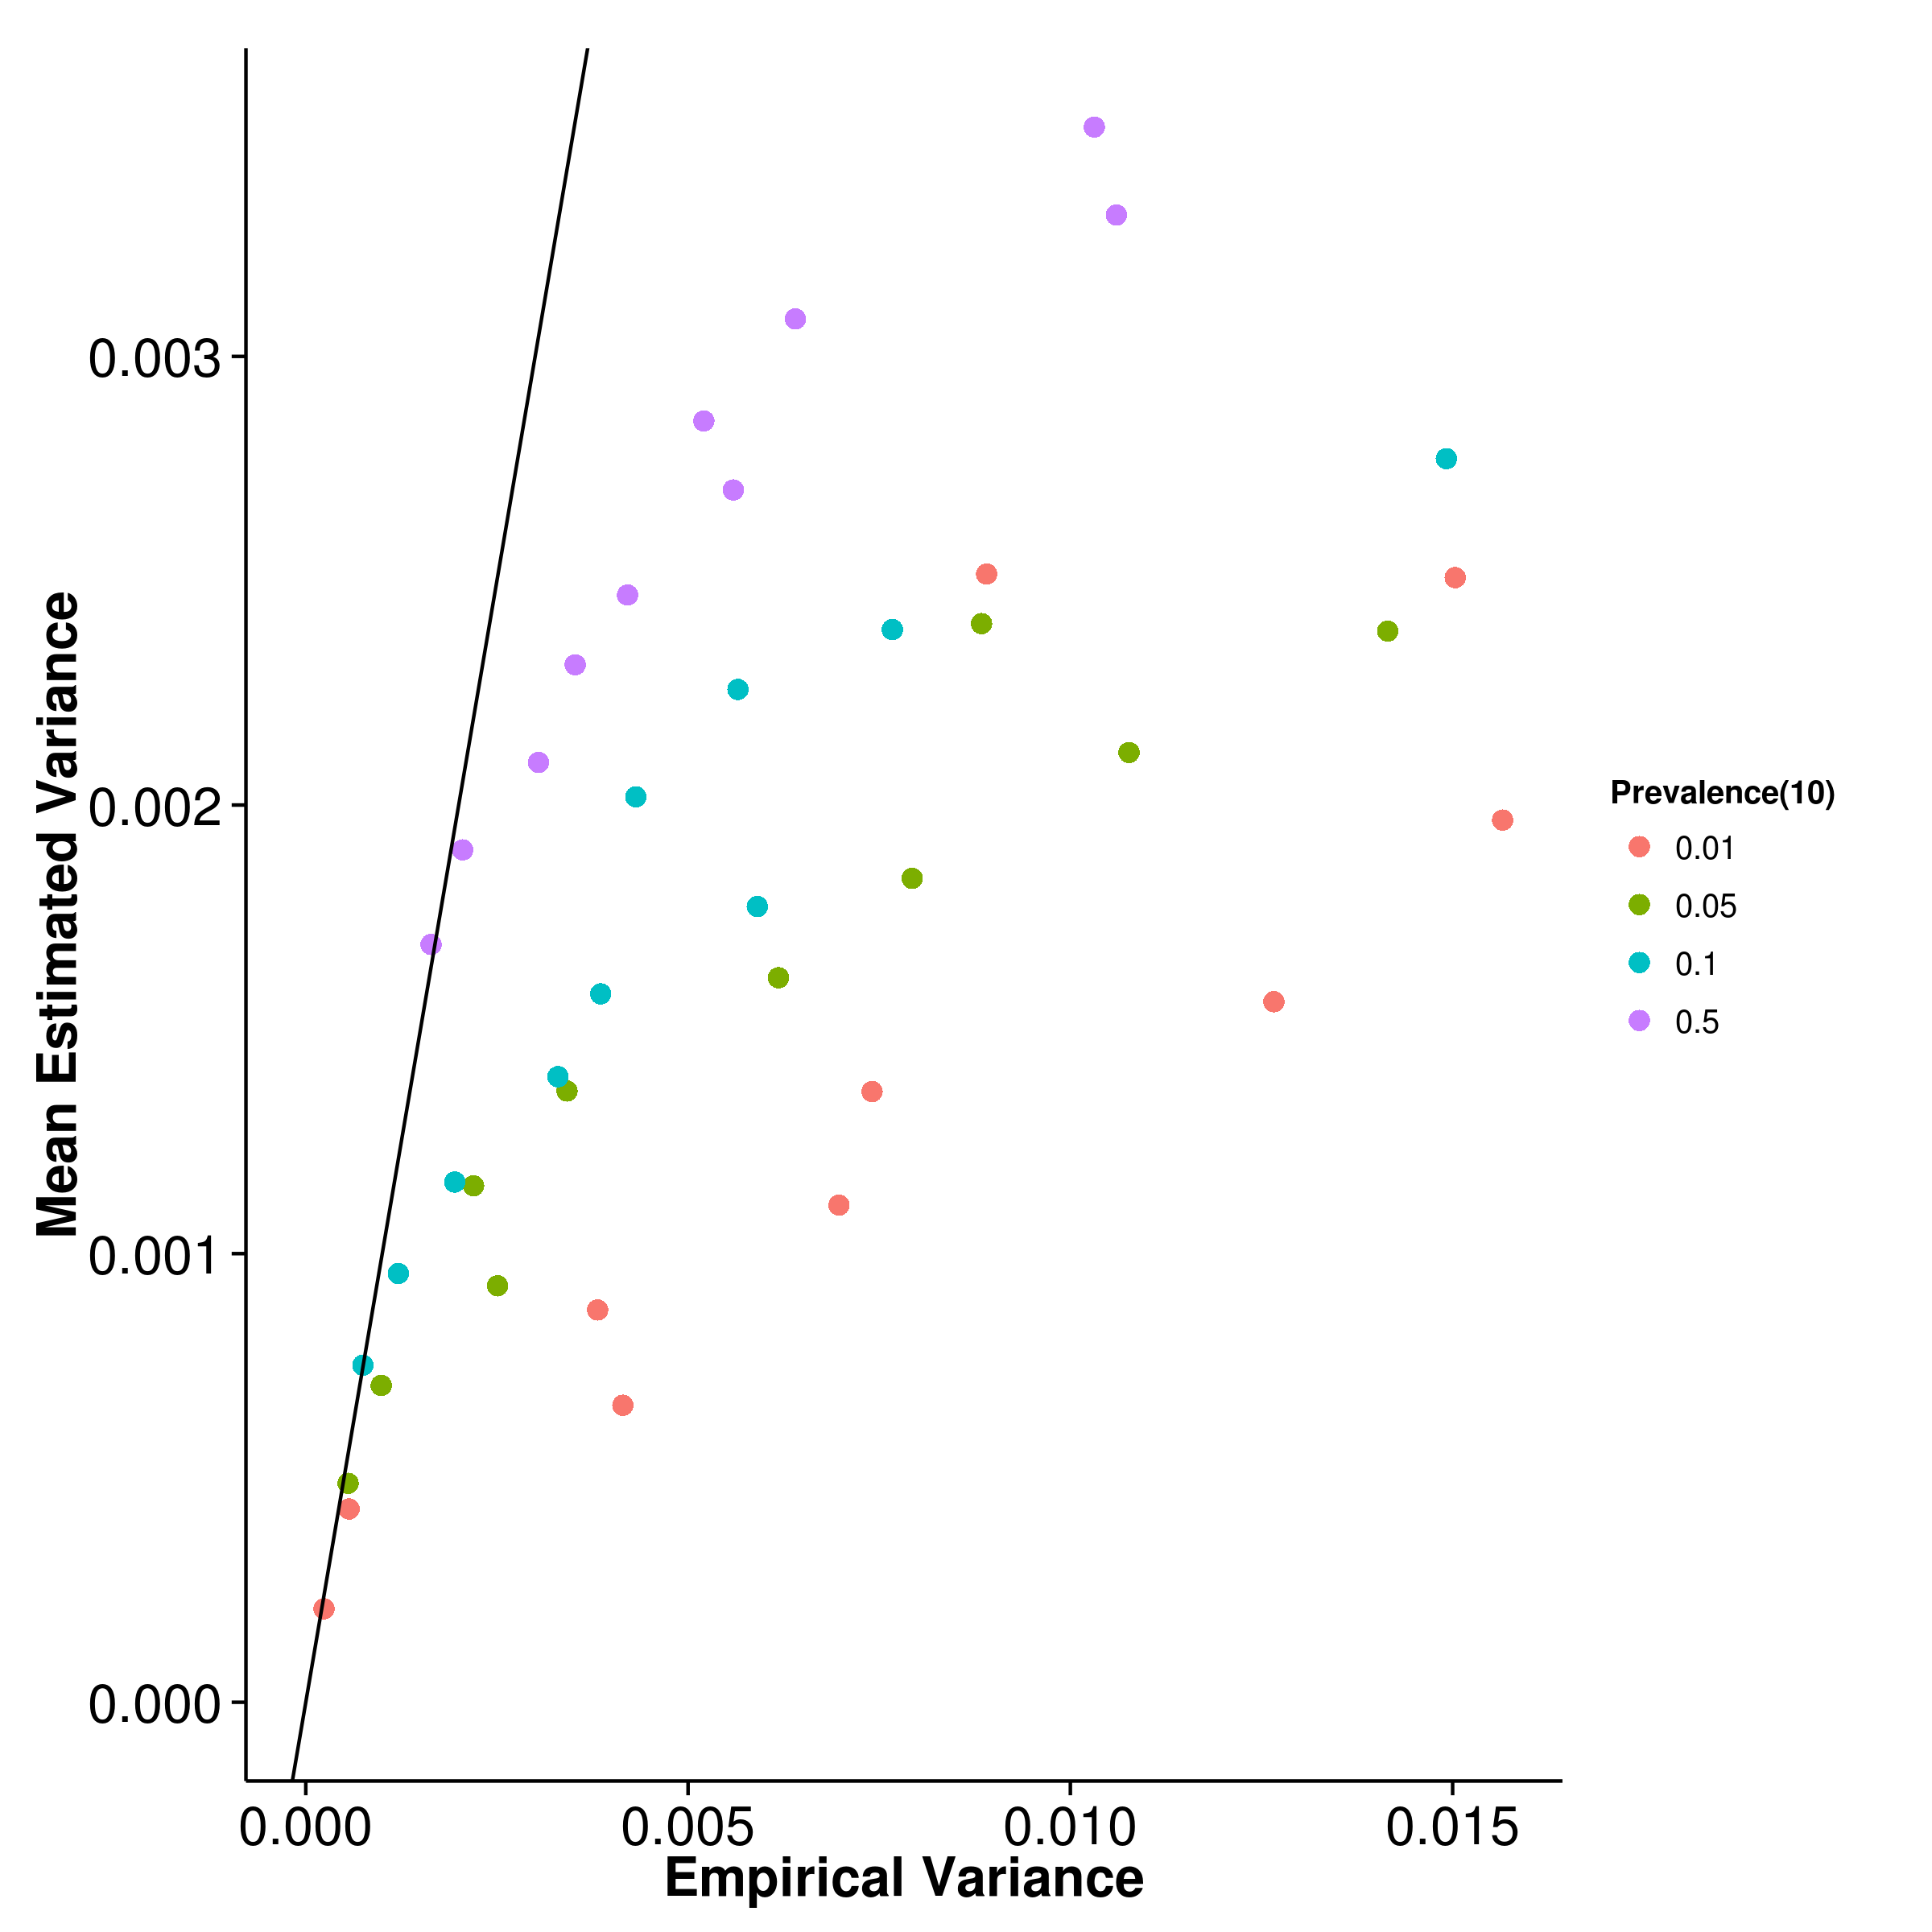
\includegraphics{figure/he_summary/cc_10c/shrek_CC_Rand_sdCom.png}}
				\label{fig:shrekCC10RandVarCom}
			}
			\subfloat[GCTA]{
				\scalebox{.4}{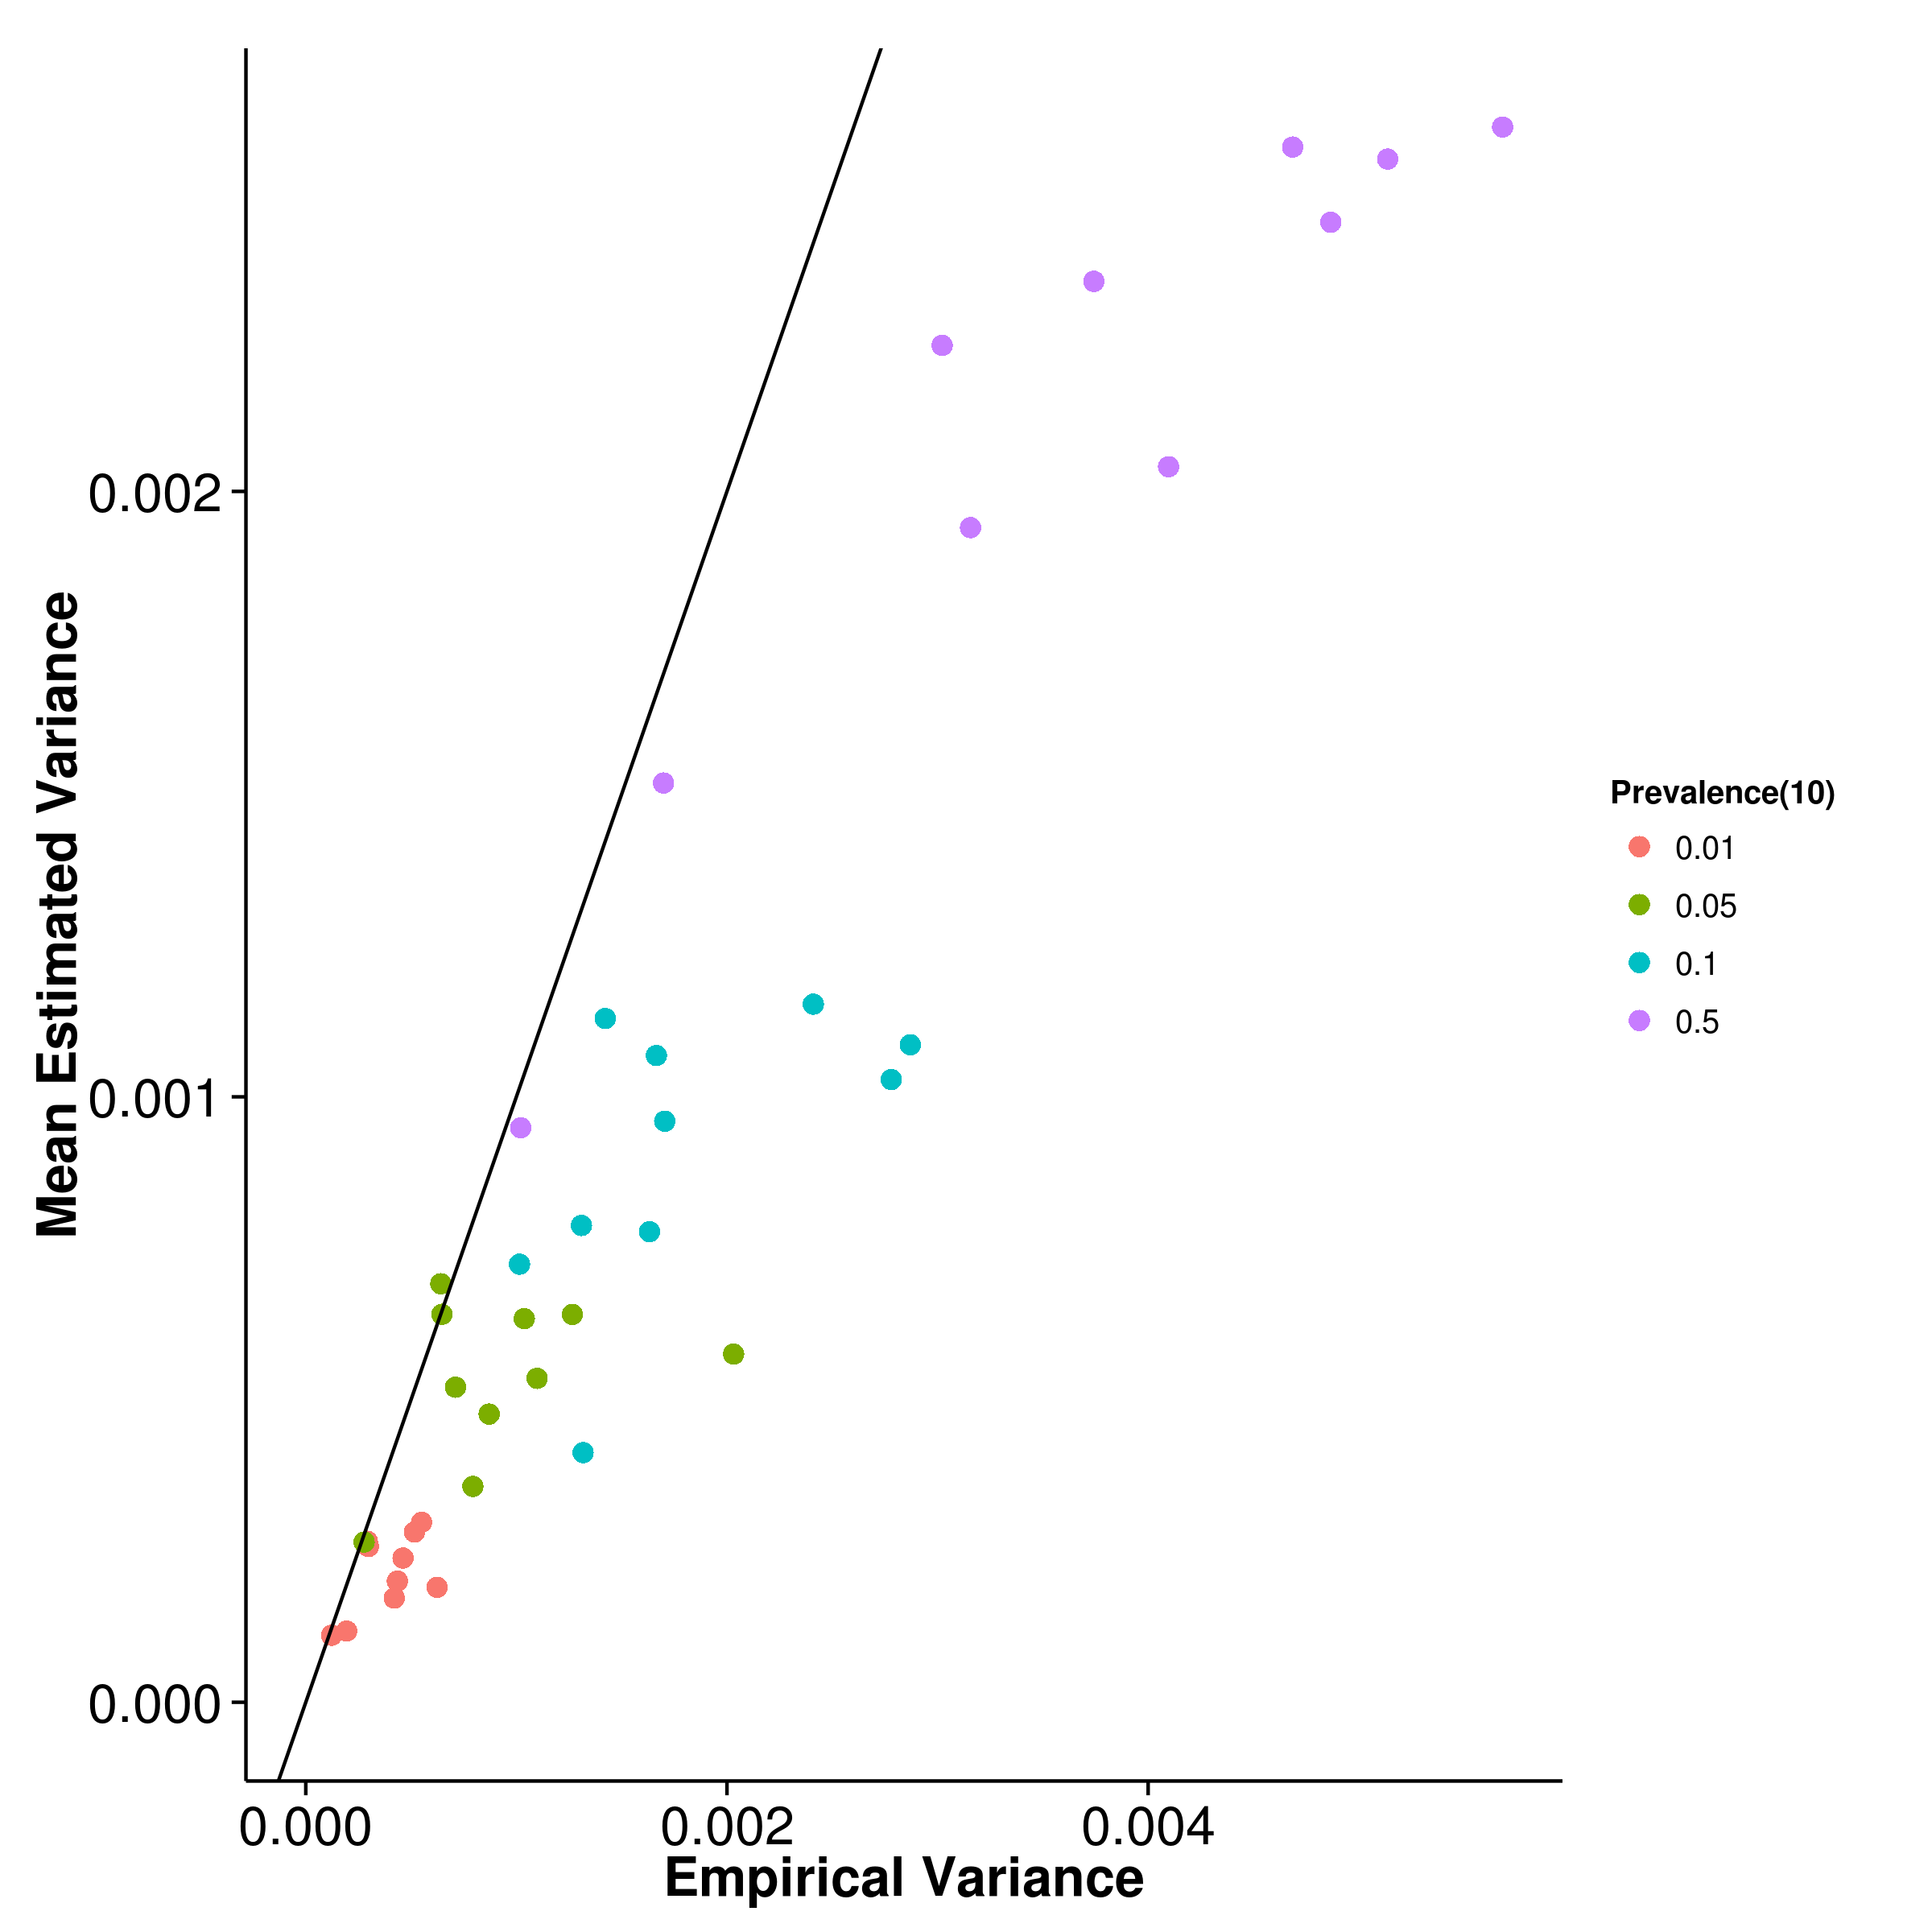
\includegraphics{figure/he_summary/cc_10c/gcta_CC_Rand_sdCom.png}}
				\label{fig:gctaCC10RandVarCom}
			}\\
			\subfloat[LDSC with fix intercept]{
				\scalebox{.4}{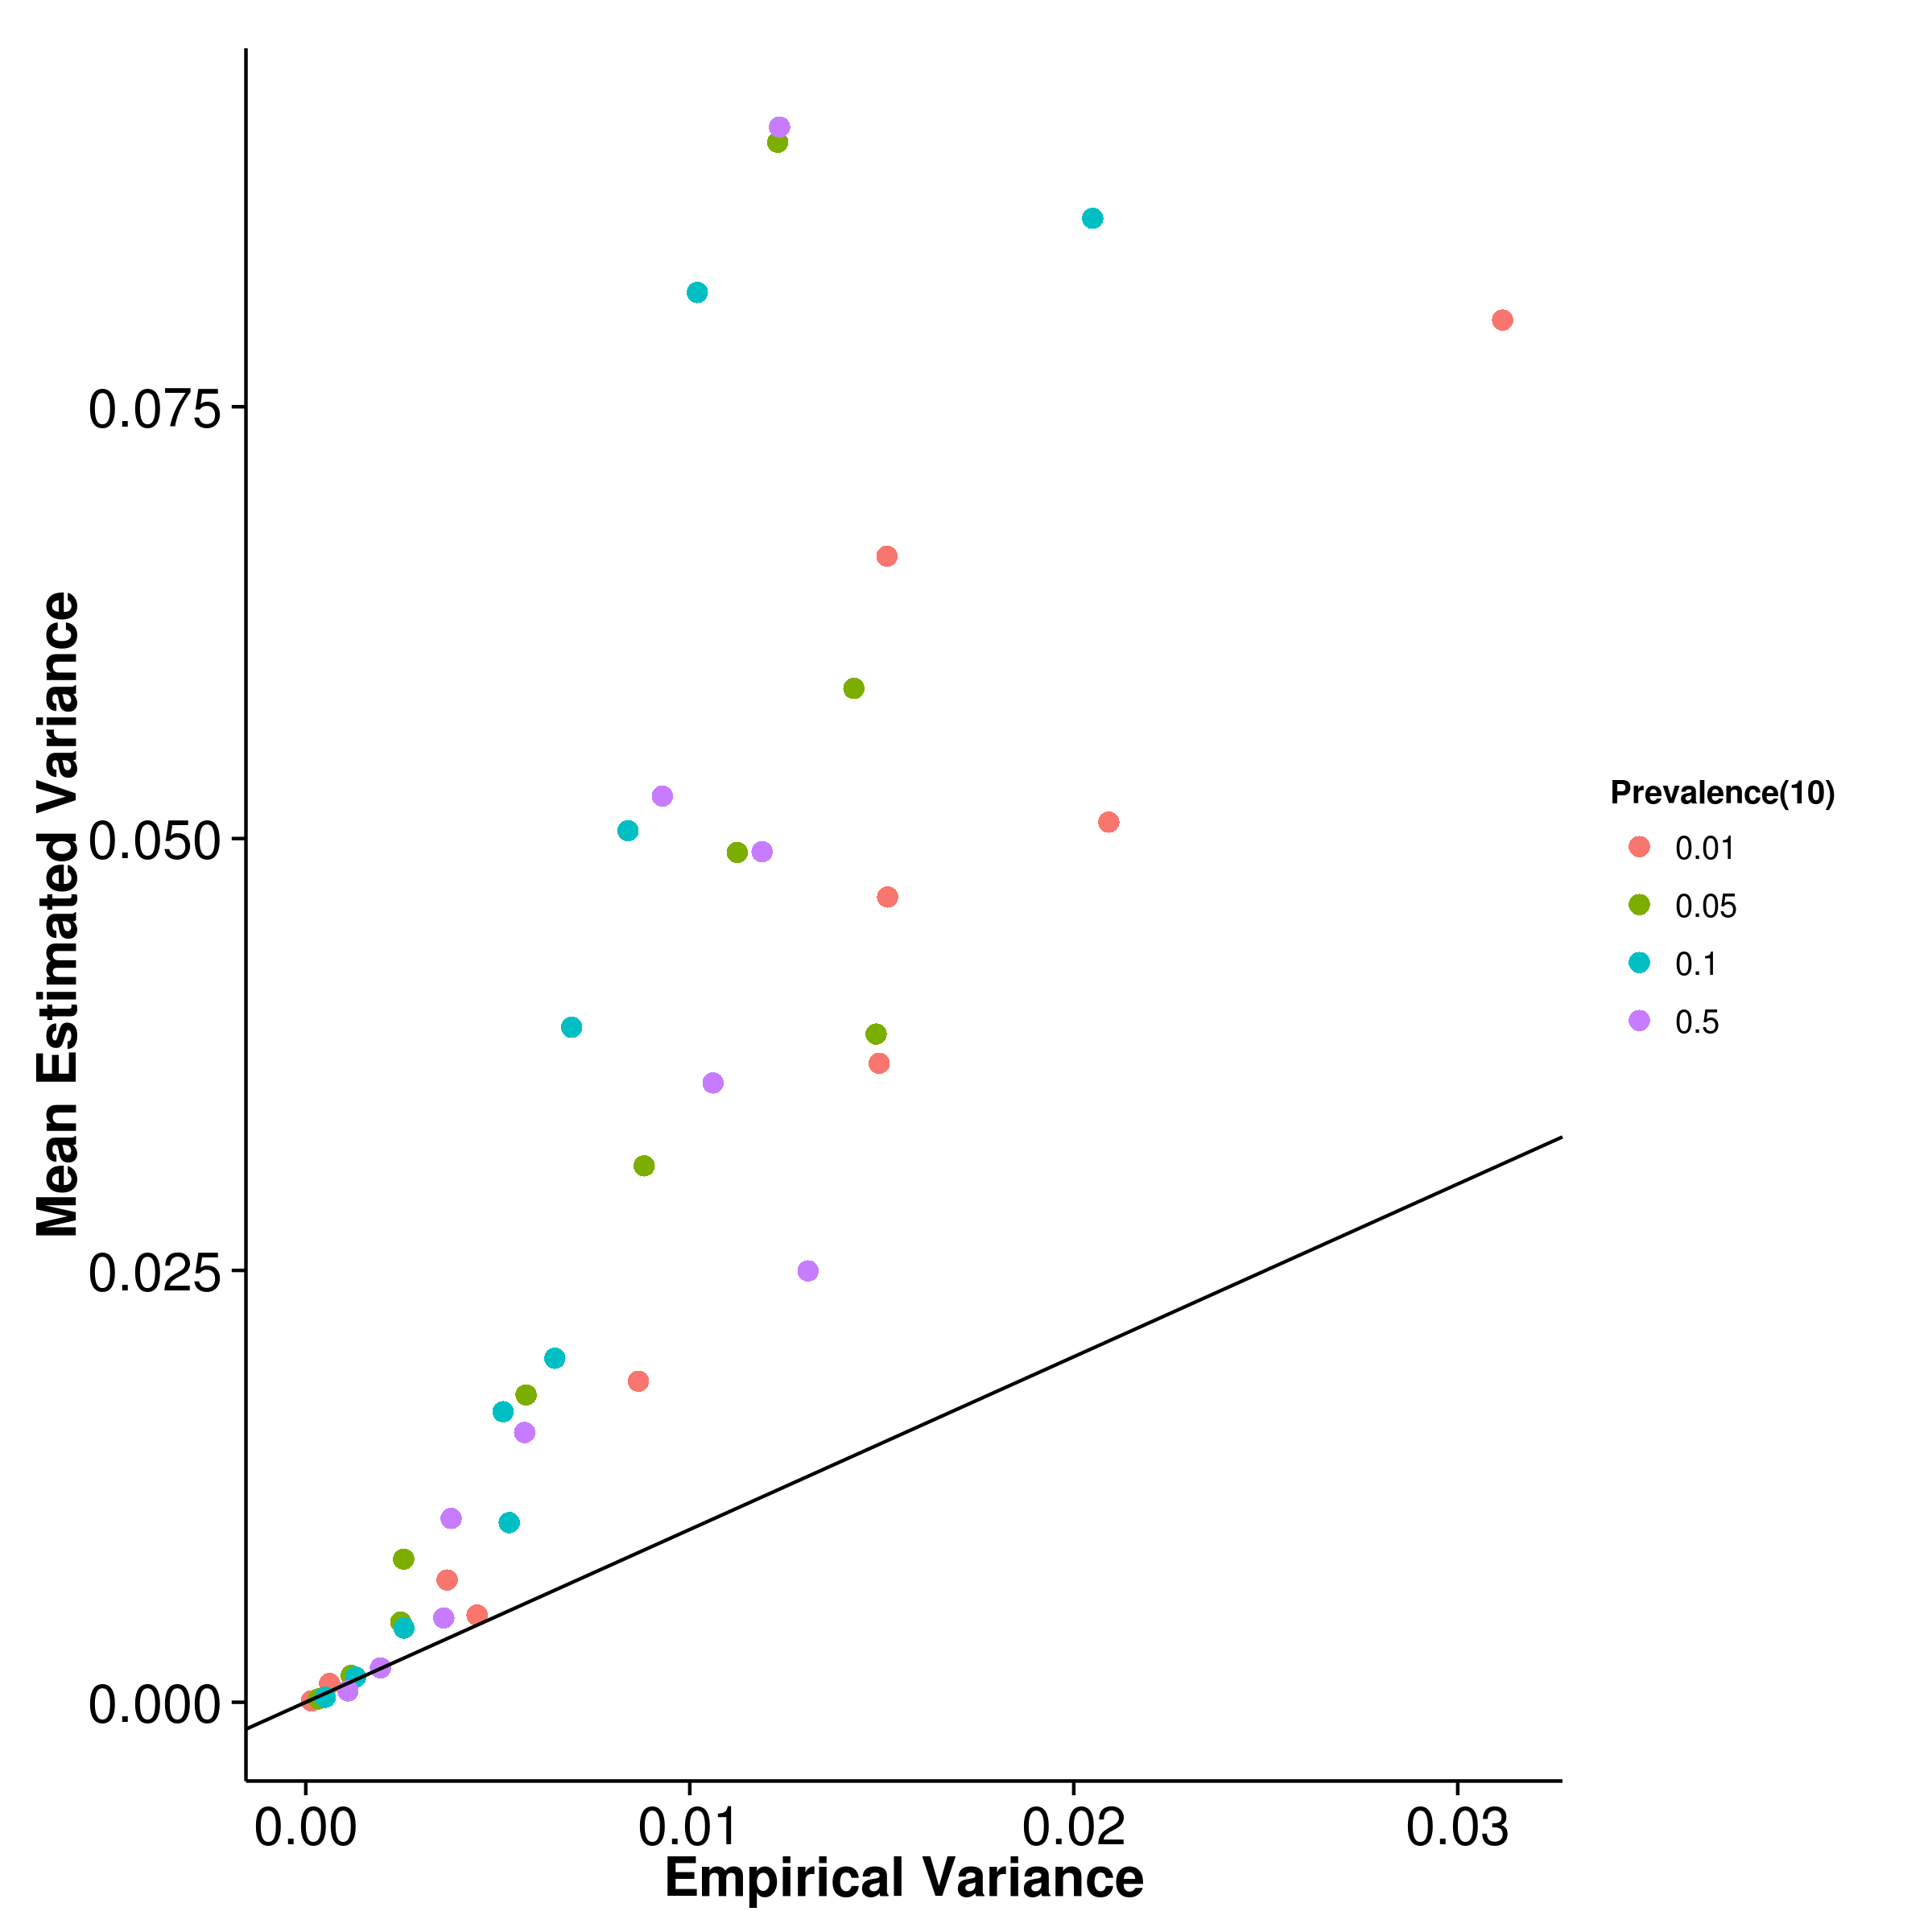
\includegraphics{figure/he_summary/cc_10c/ldsc_CC_Rand_sdCom.png}}
				\label{fig:ldscCC10RandVarCom}
			}
			\subfloat[LDSC with intercept estimation]{
				
				\scalebox{.4}{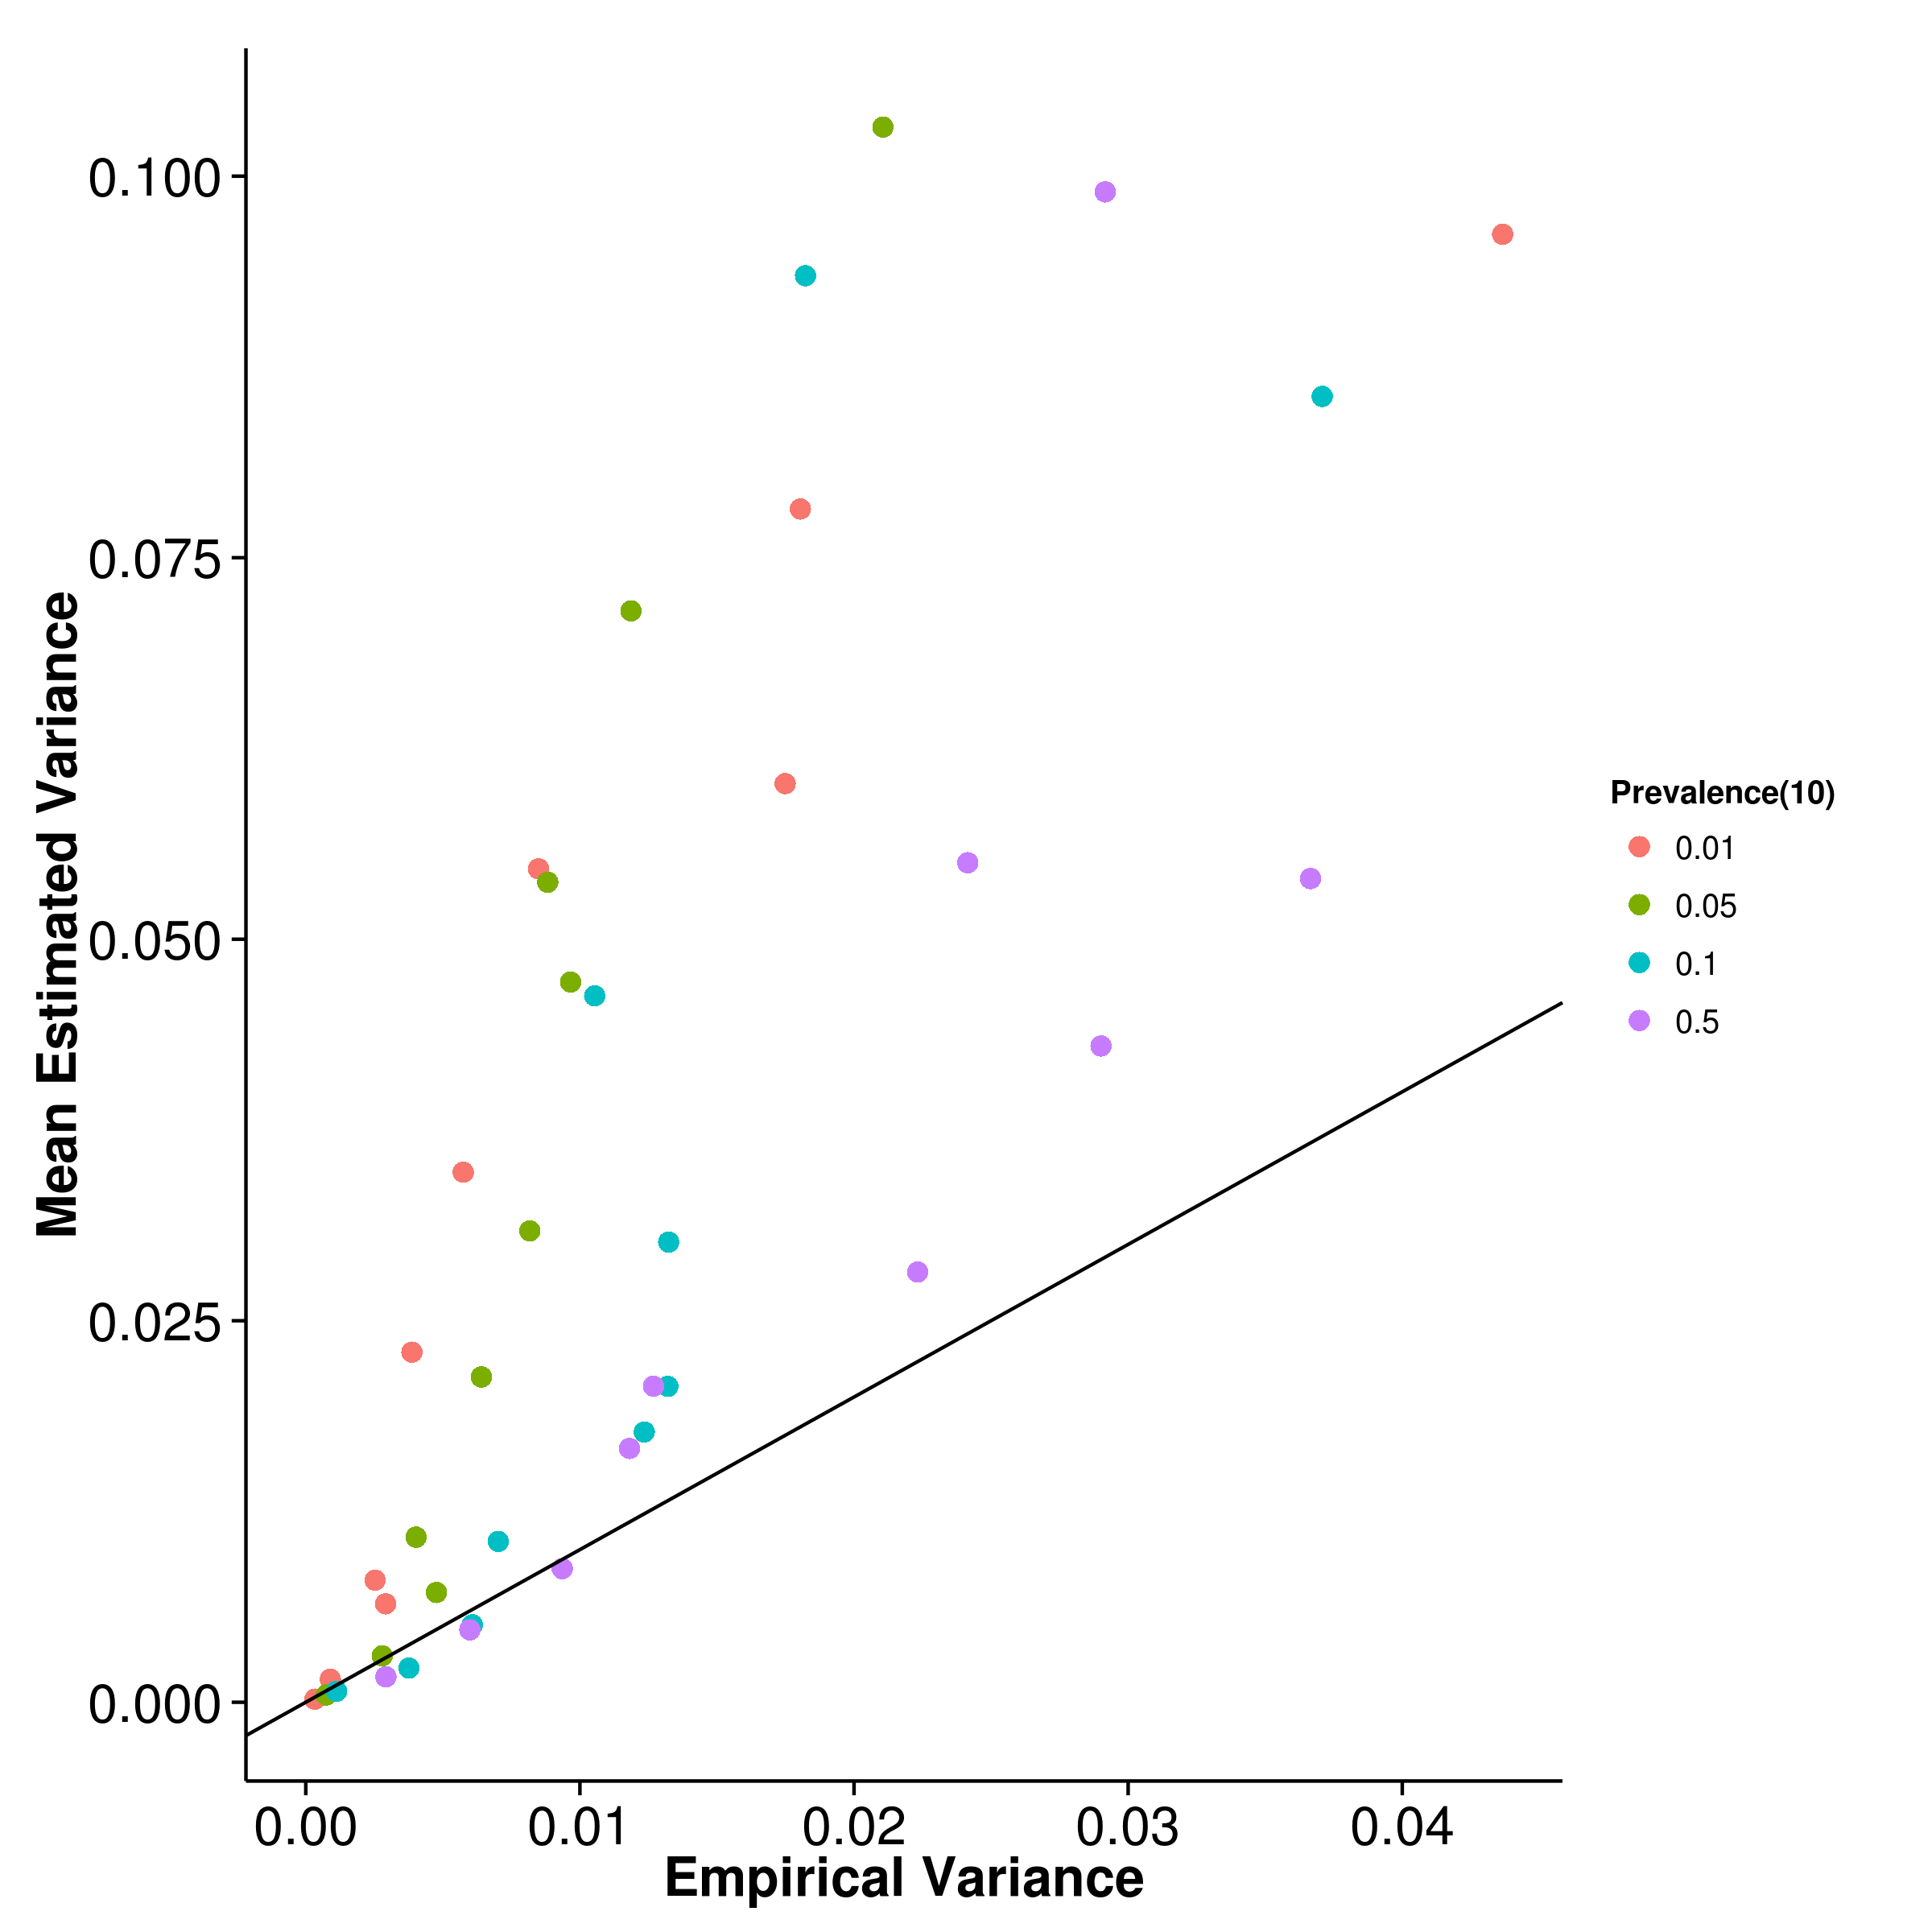
\includegraphics{figure/he_summary/cc_10c/ldscIn_CC_Rand_sdCom.png}}
				\label{fig:ldscInCC10RandVarCom}
			}
			\caption[Estimation of Variance in Case Control Simulation (10 Causal)]
			{Estimated variance of results from case control simulation with random effect size simulation when compared to empirical variance when 10 causal \glspl{SNP} was simulated.
				A general underestimation was observed for \gls{shrek} and \gls{gcta} whereas a larger upward bias was observed for \gls{ldsc}.} 
			\label{fig:CC10RandVarCom}
		\end{figure}
		

	\begin{figure}[H]
			\centering
			\subfloat[SHREK]{
				\scalebox{.4}{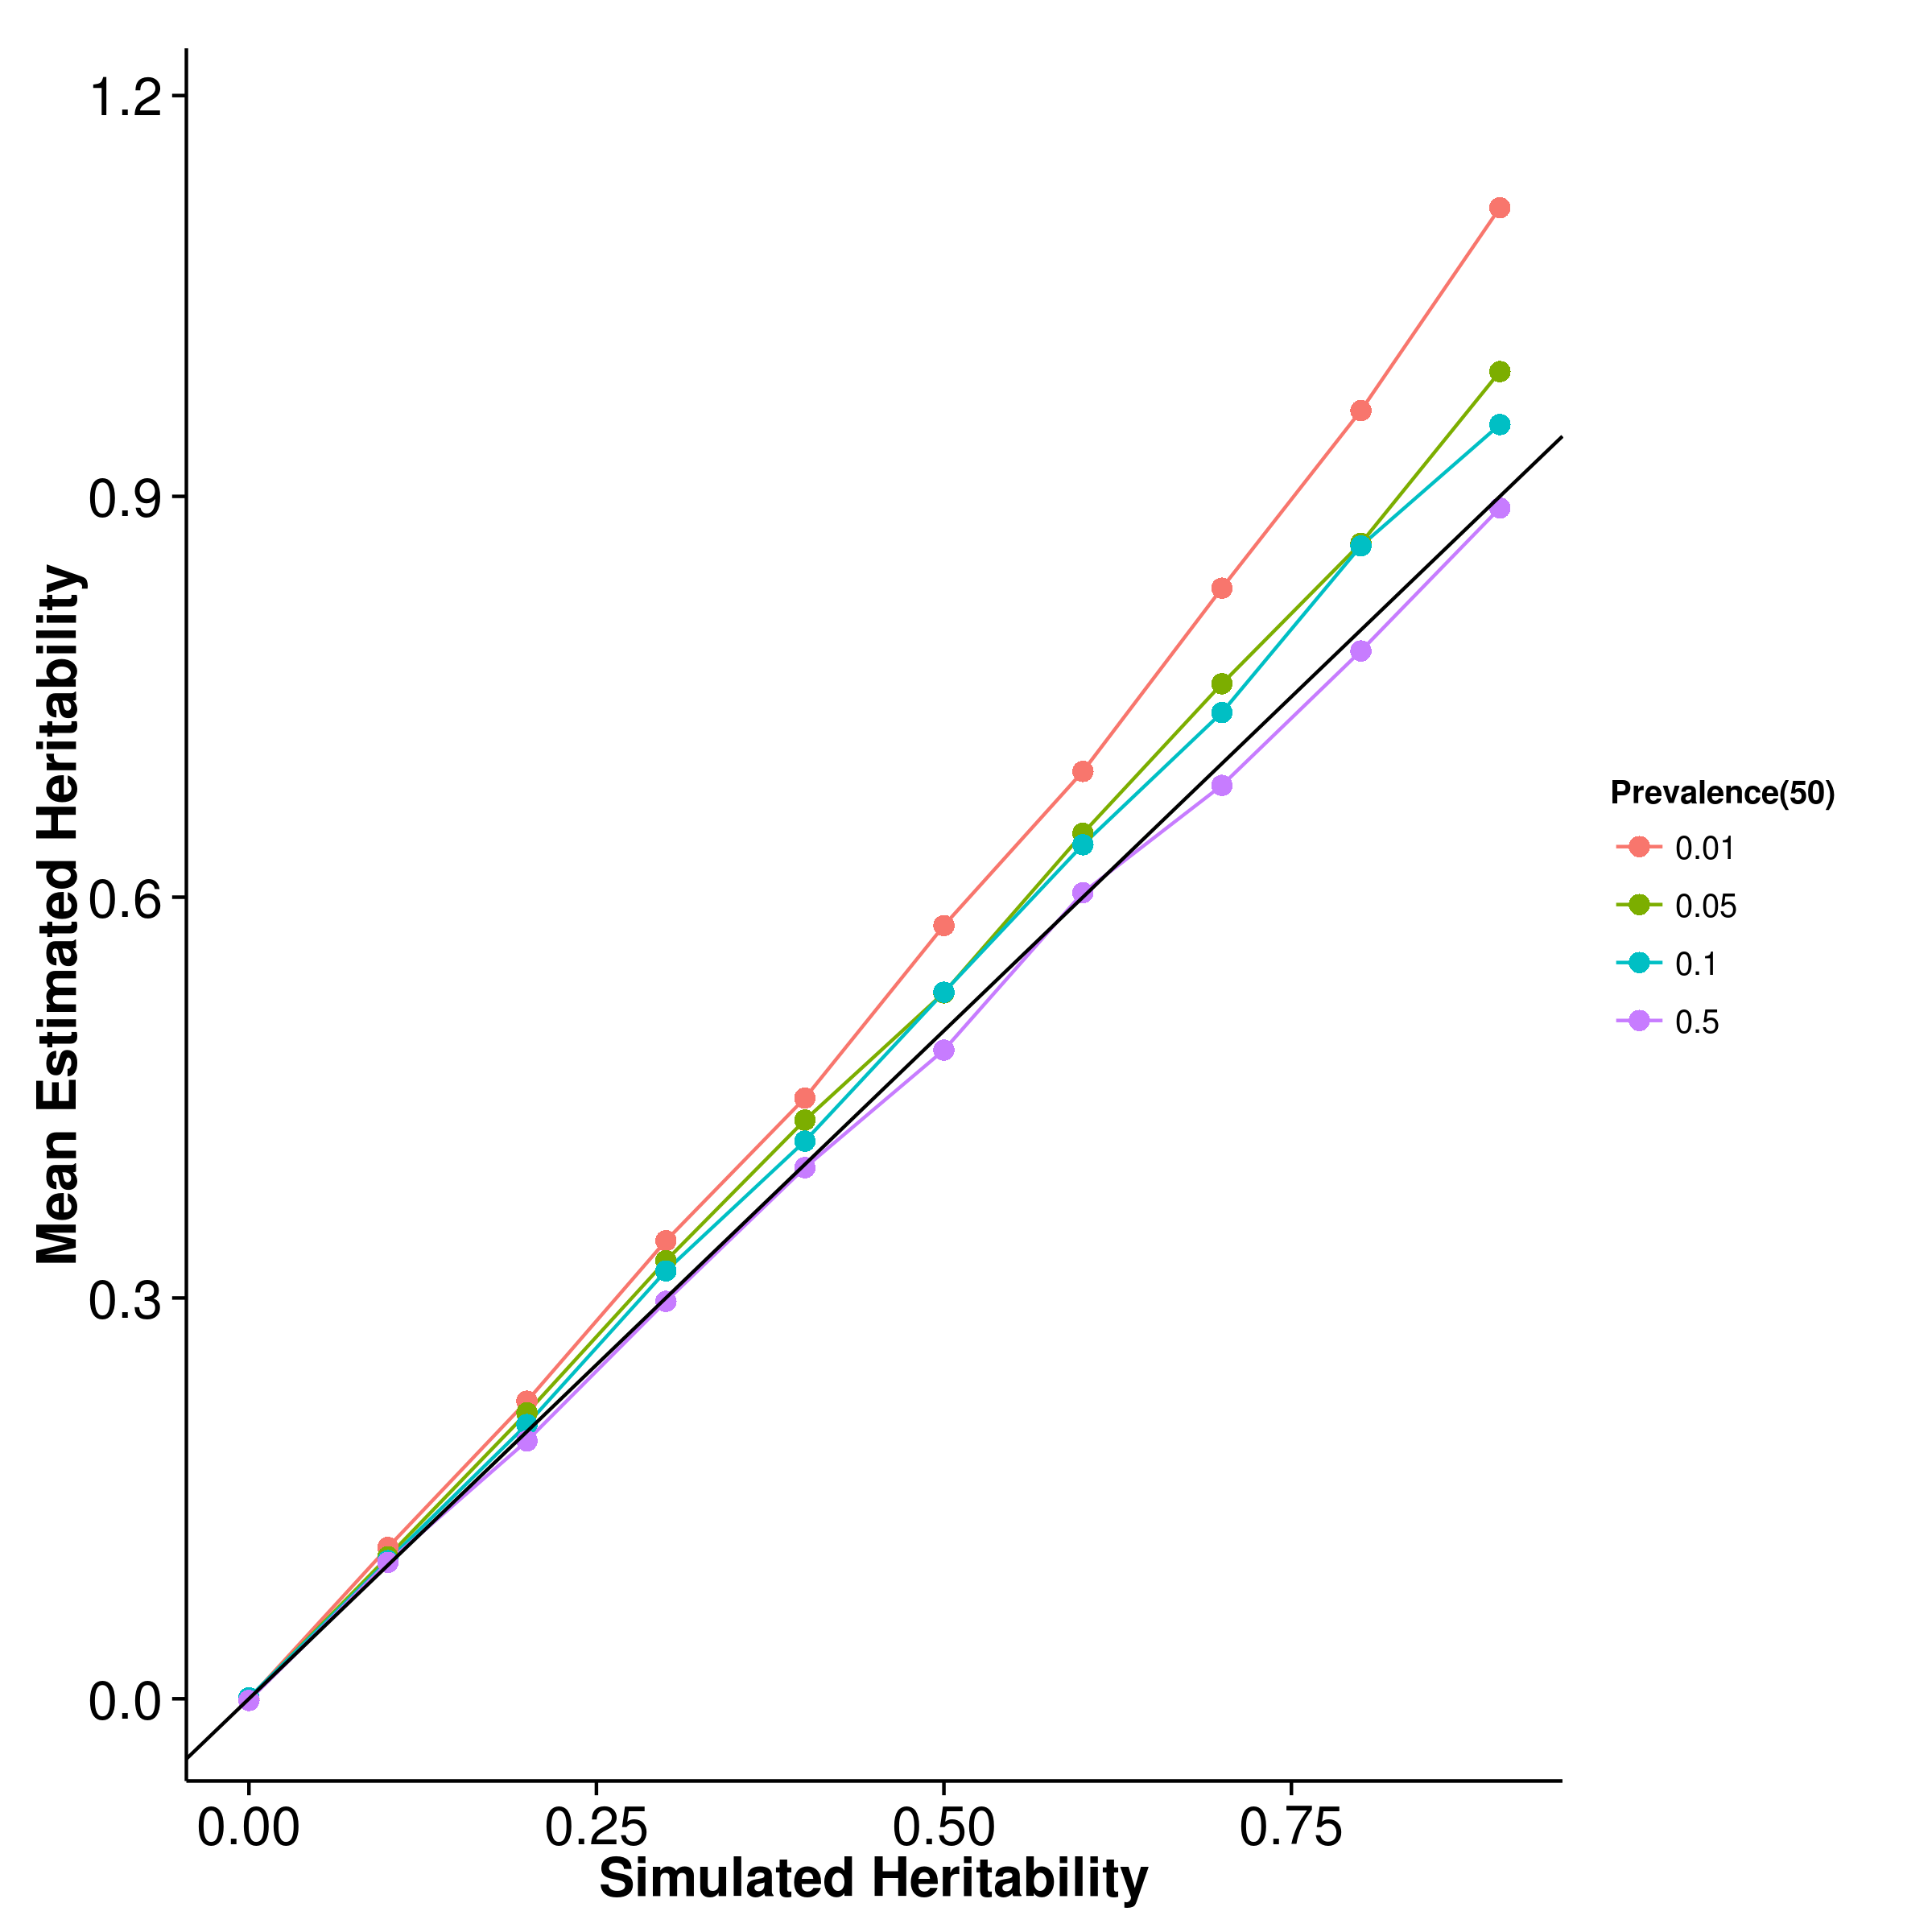
\includegraphics{figure/he_summary/cc_50c/shrek_CC_Rand_mean.png}}
				\label{fig:shrekCC50RandMean}
			}
			\subfloat[GCTA]{
				\scalebox{.4}{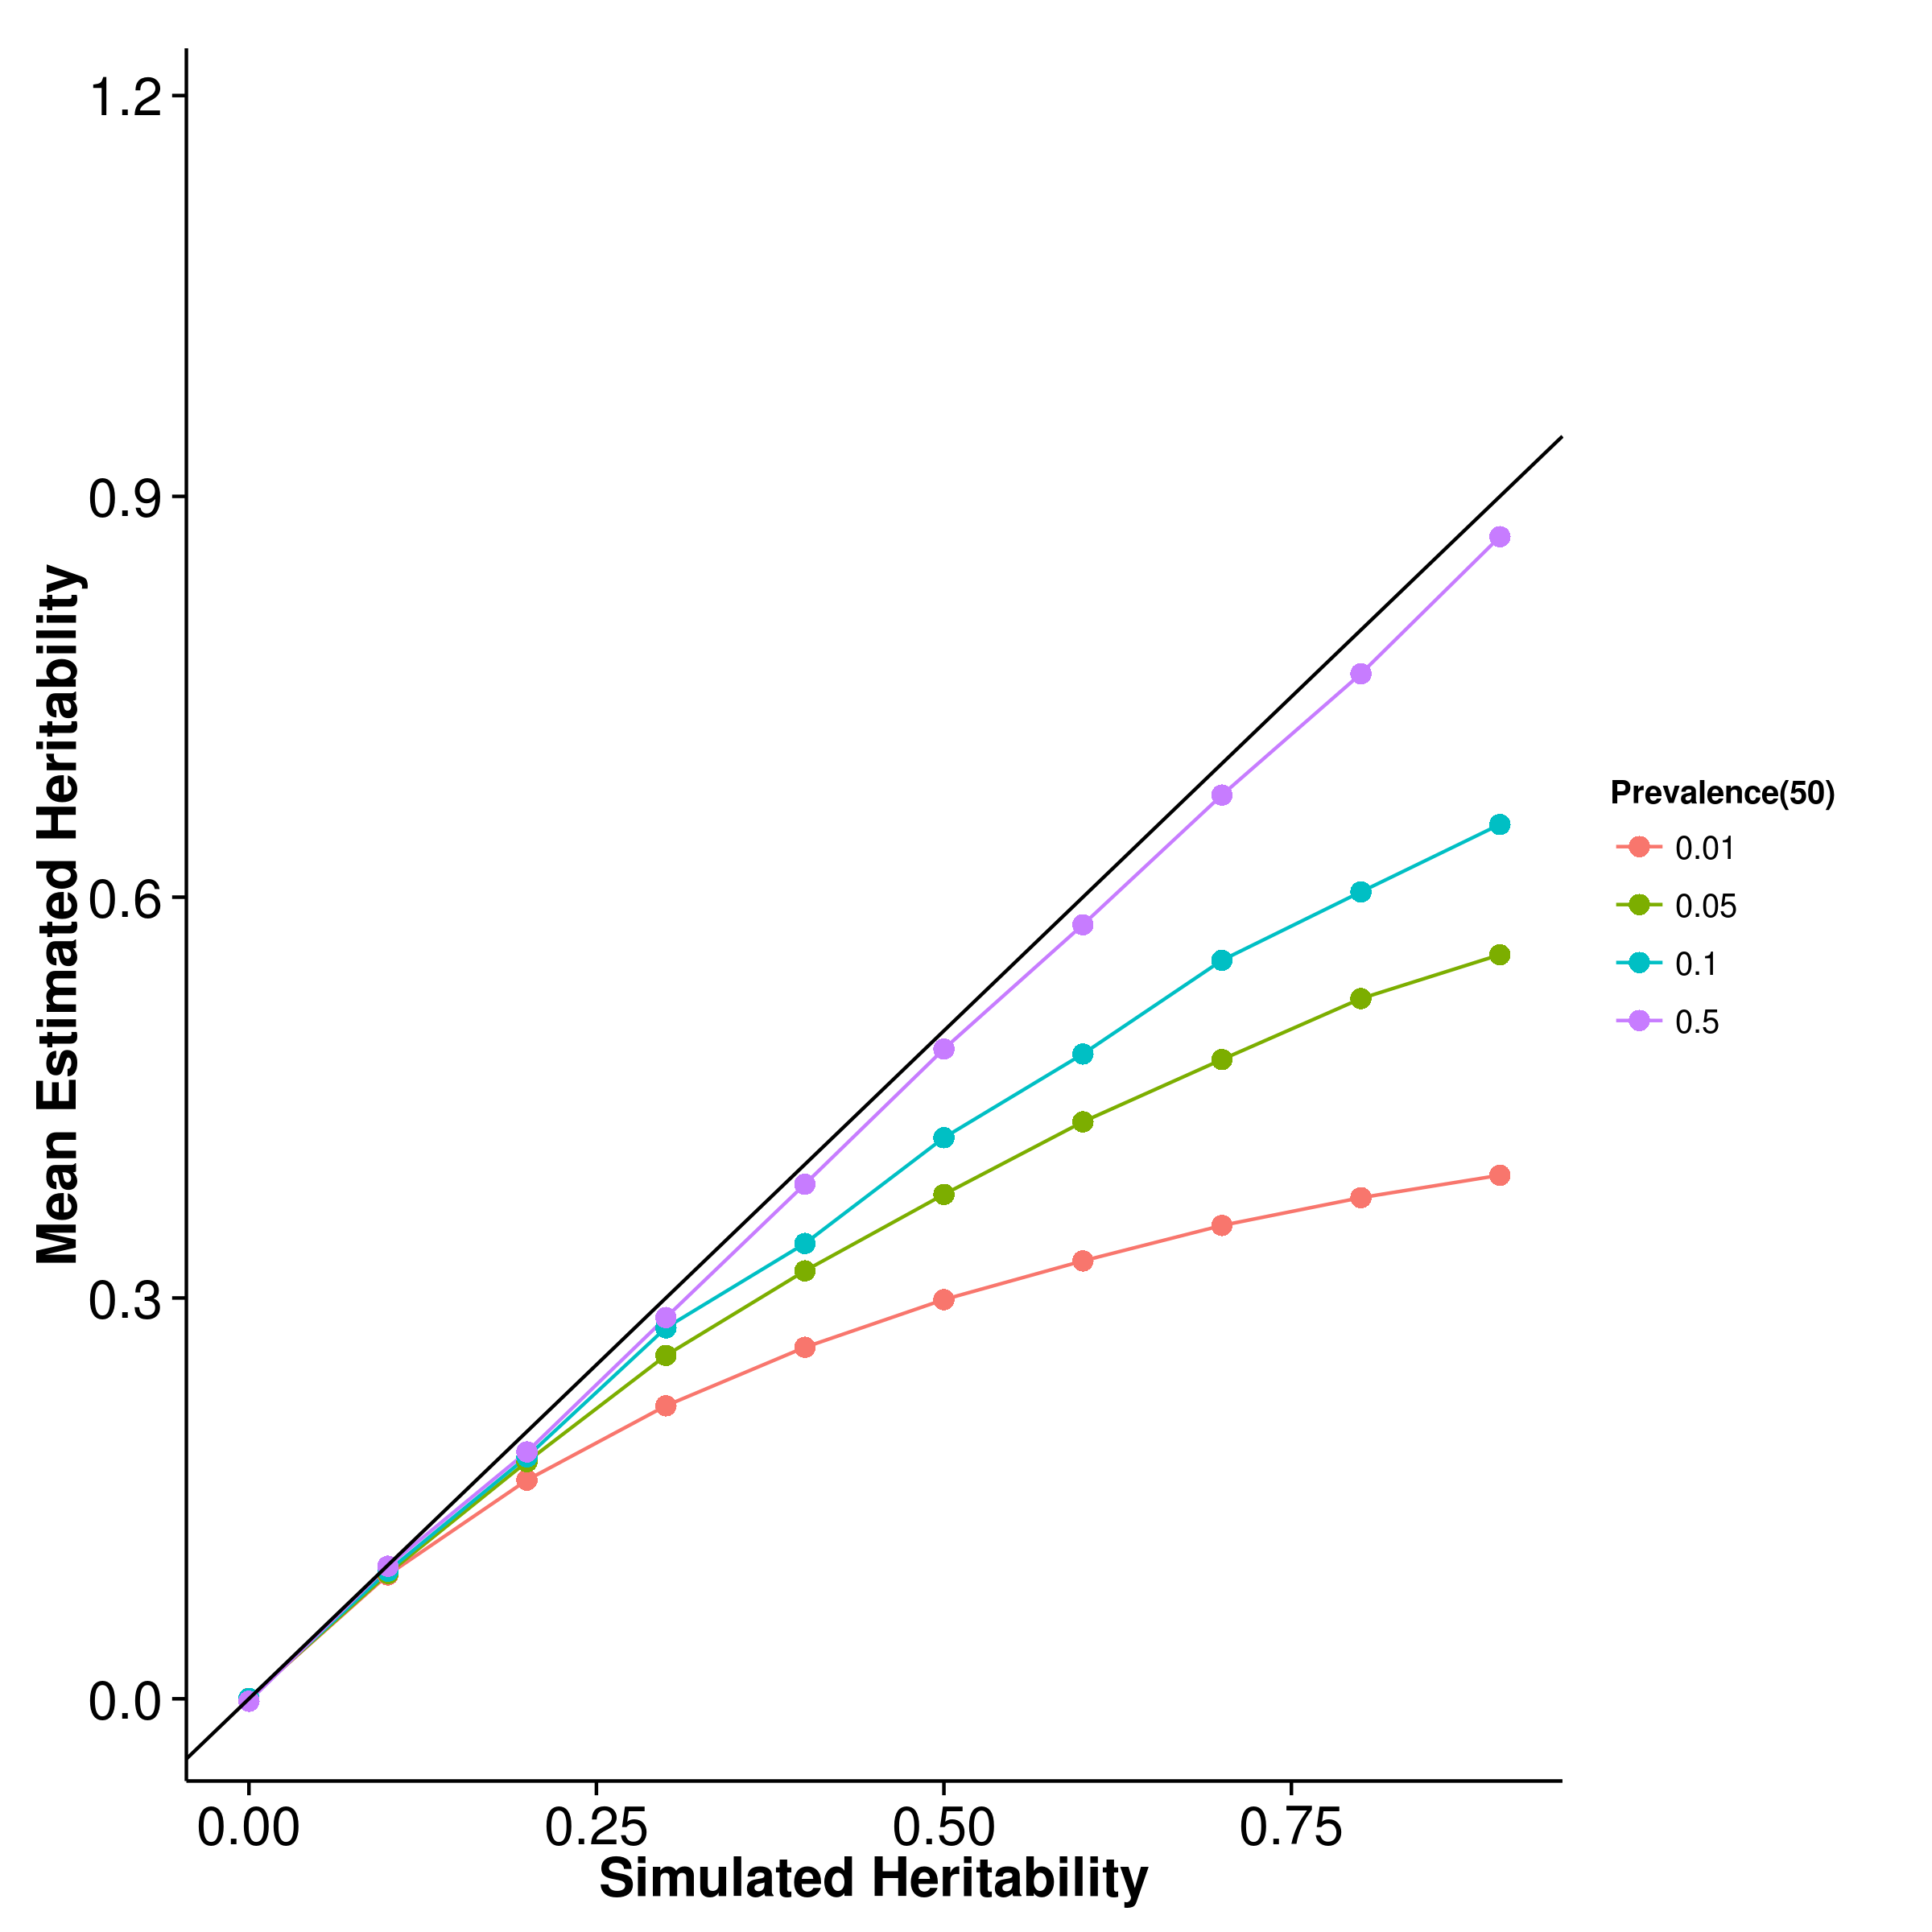
\includegraphics{figure/he_summary/cc_50c/gcta_CC_Rand_mean.png}}
				\label{fig:gctaCC50RandMean}
			}\\
			\subfloat[LDSC with fix intercept]{
				\scalebox{.4}{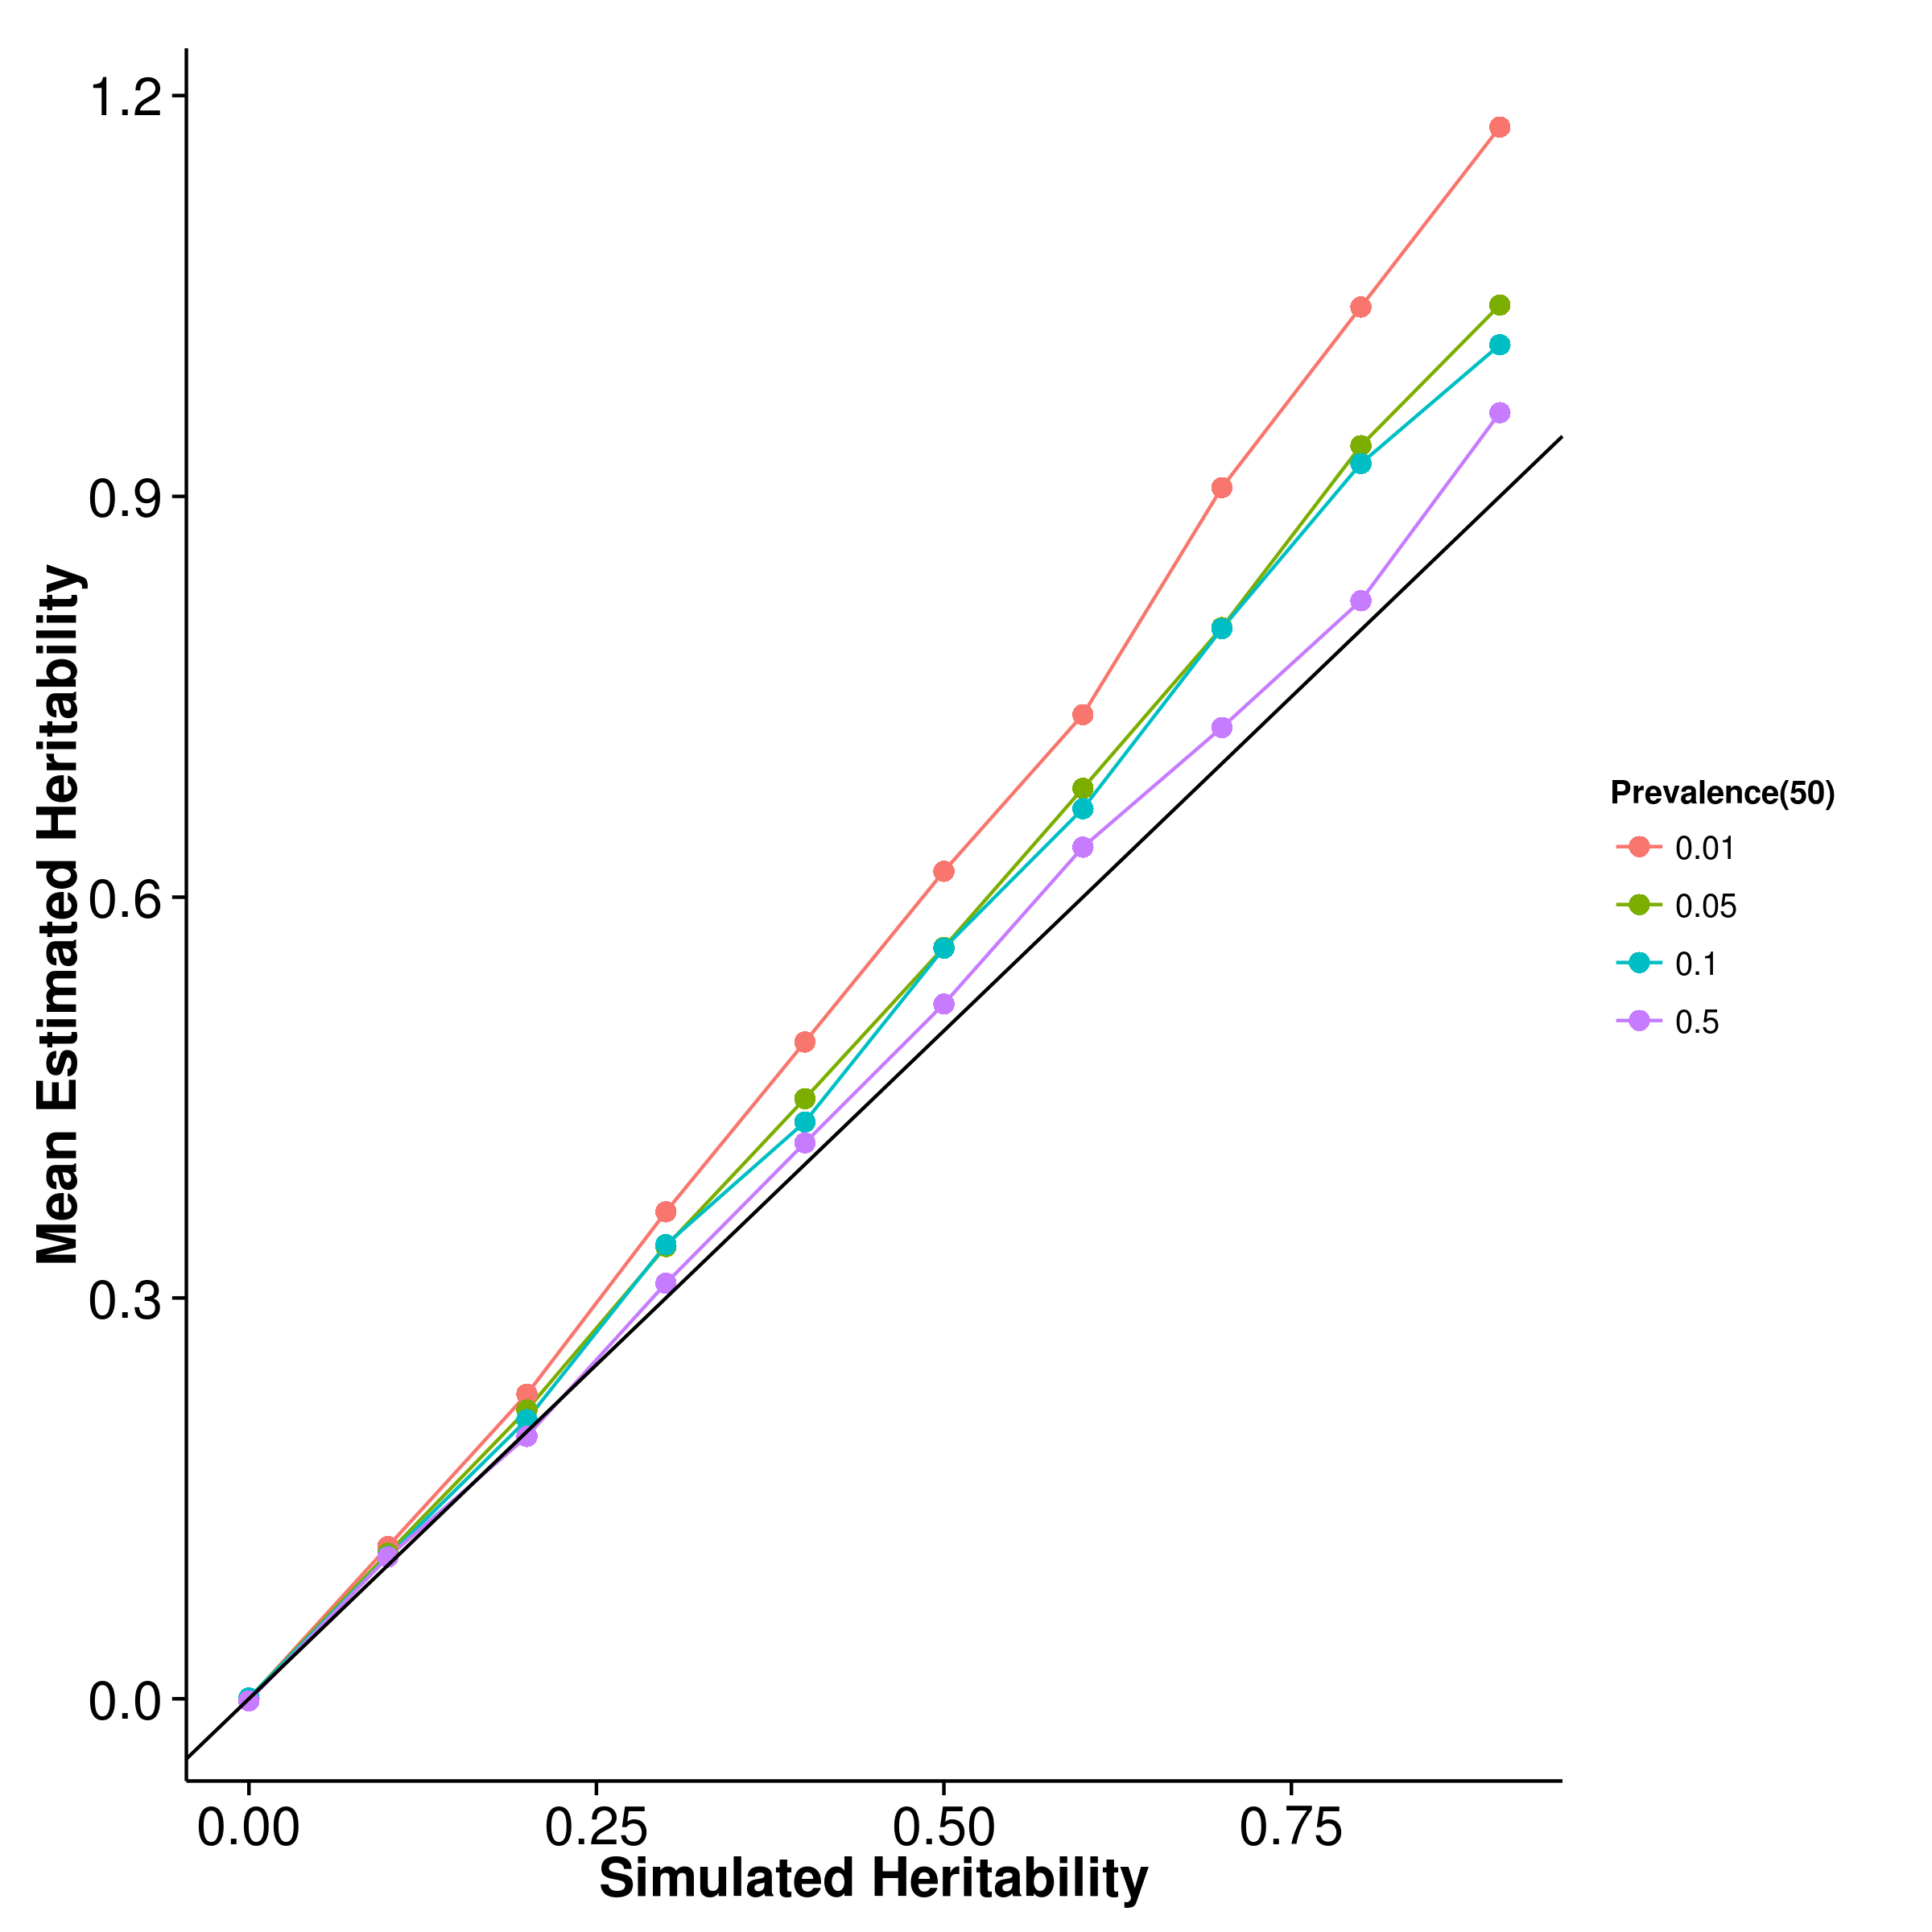
\includegraphics{figure/he_summary/cc_50c/ldsc_CC_Rand_mean.png}}
				\label{fig:ldscCC50RandMean}
			}
			\subfloat[LDSC with intercept estimation]{
				
				\scalebox{.4}{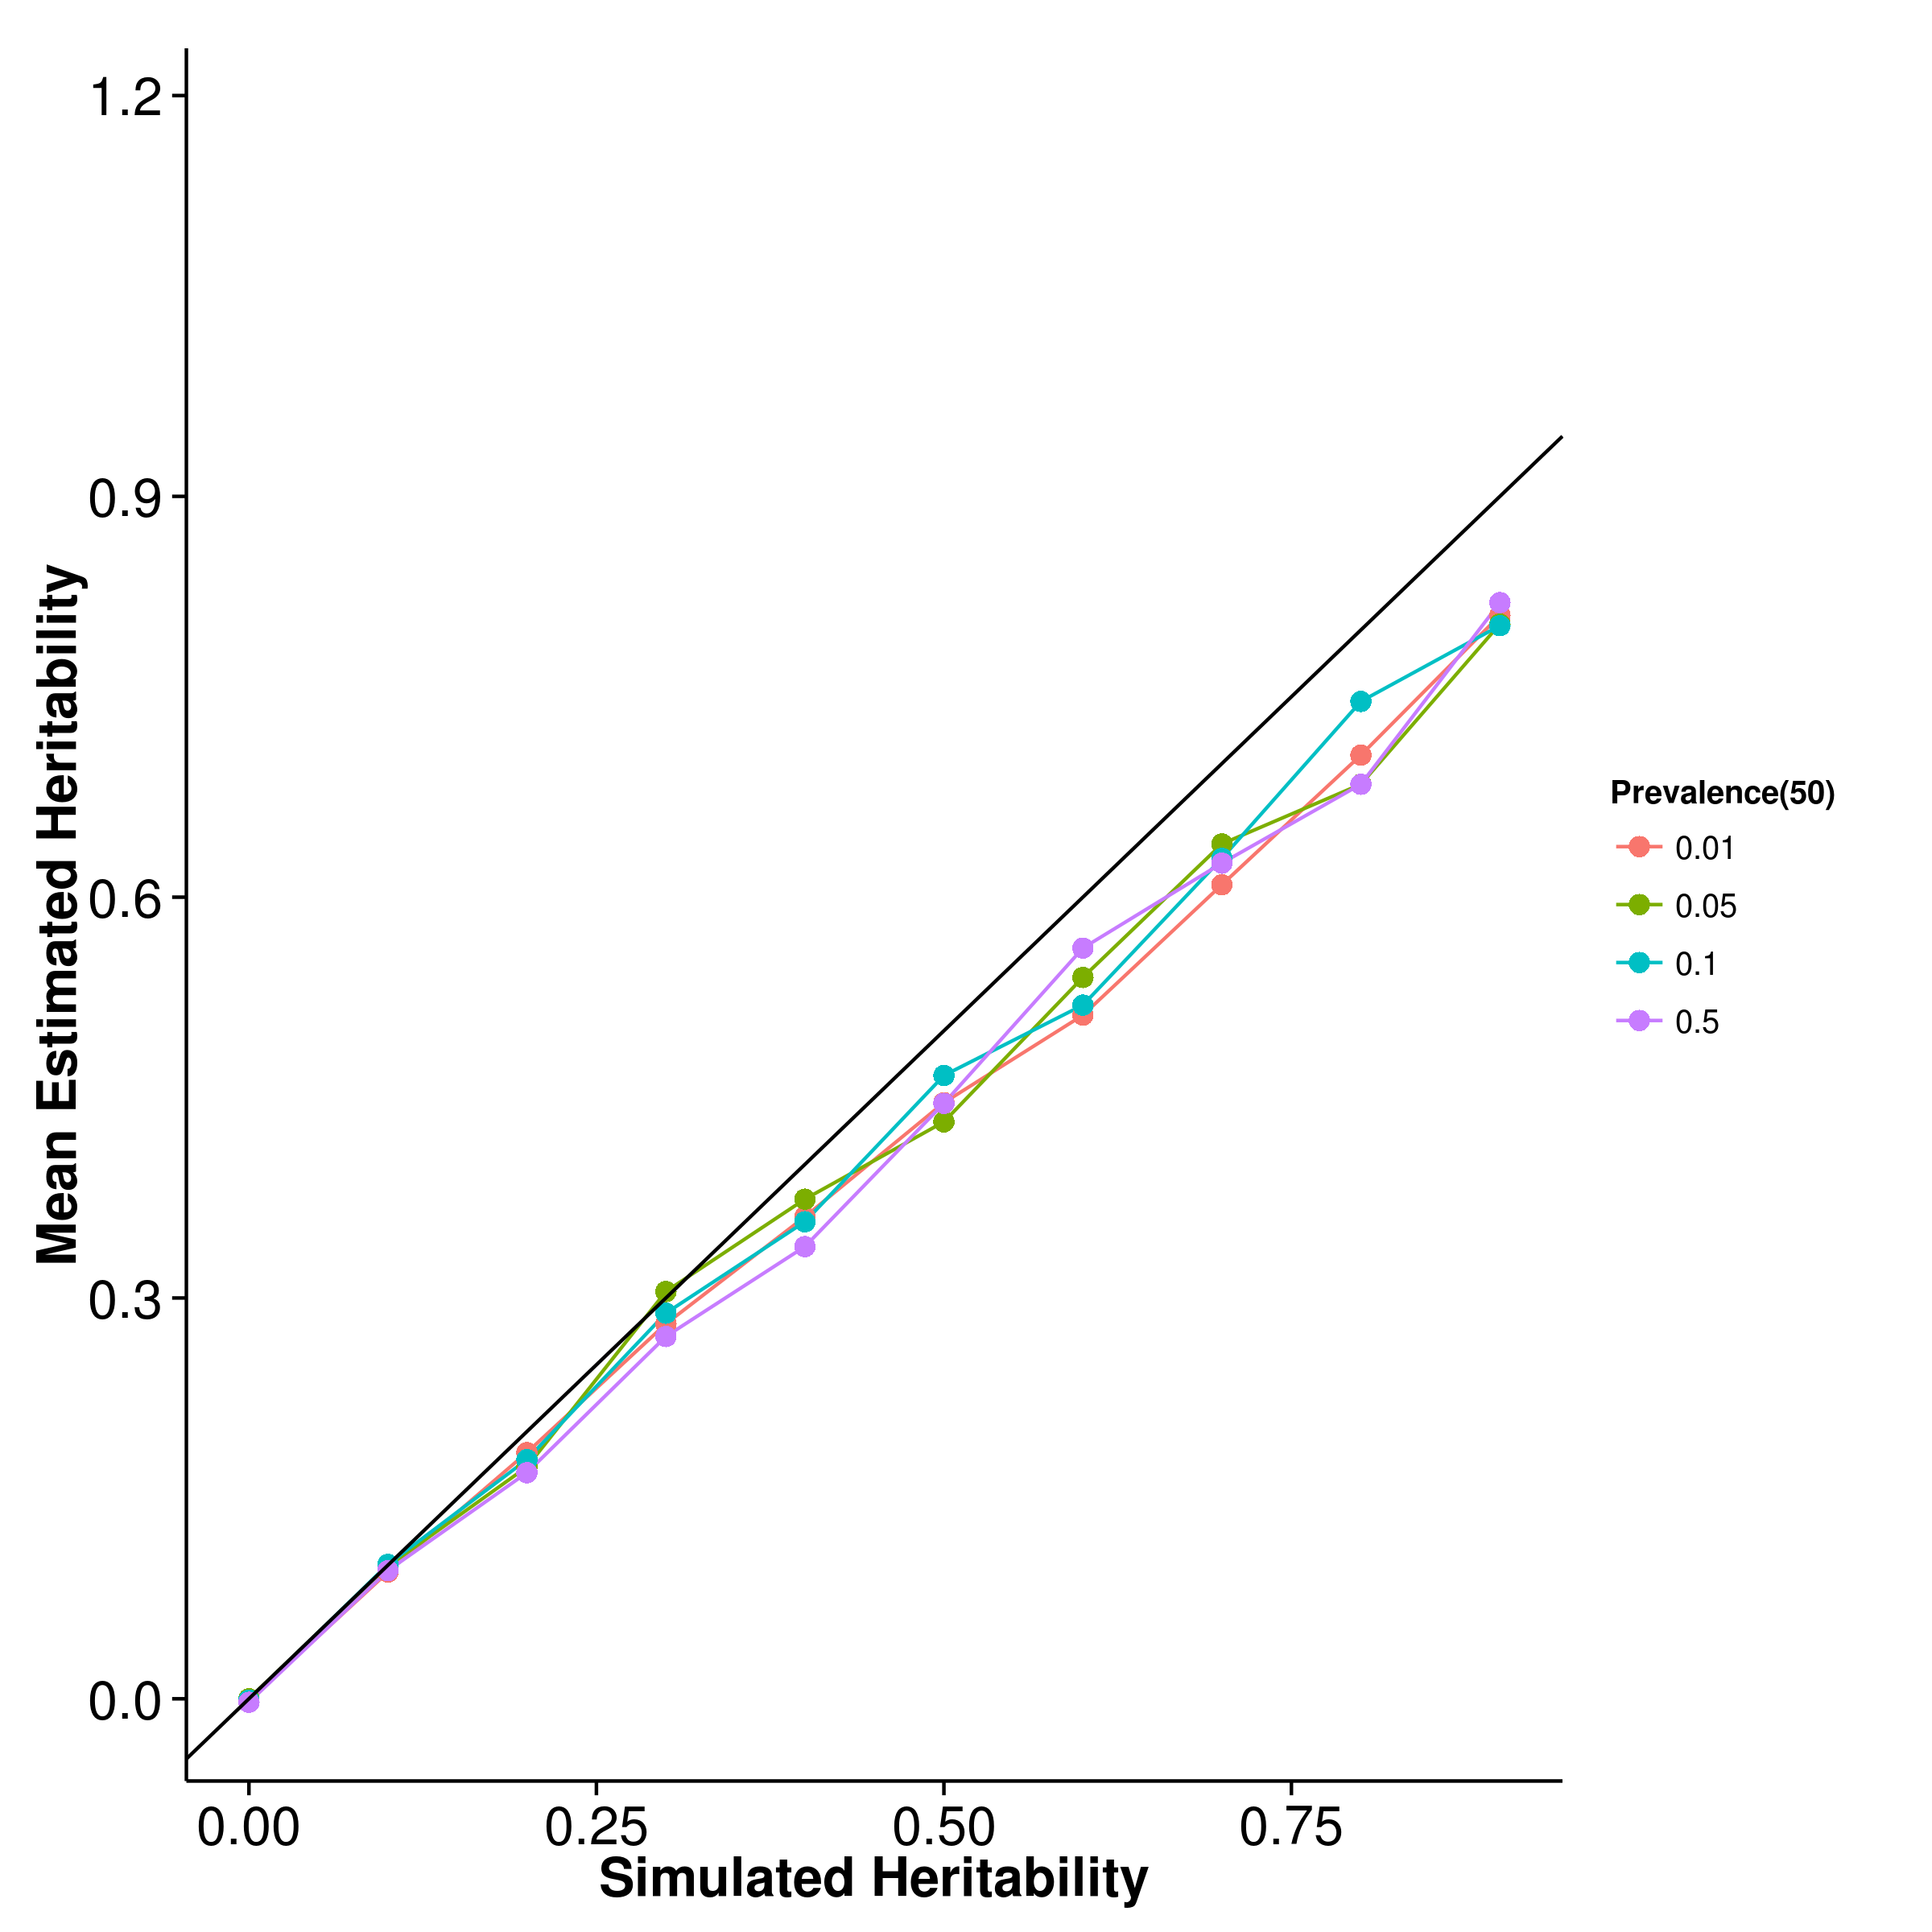
\includegraphics{figure/he_summary/cc_50c/ldscIn_CC_Rand_mean.png}}
				\label{fig:ldscInCC50RandMean}
			}
			\caption[Mean of Case Control Simulation Results (50 Causal)]
			{Mean of results from case control simulation with random effect size simulation with 50 causal \glspl{SNP}.
				In general, the results were similar to the scenario with 10 causal \glspl{SNP} with the only exception that the estimates from \gls{ldsc} with intercept estimates seems to be less affected by the change in prevalence of the trait.
				} 
			\label{fig:CC50RandMean}
		\end{figure}
		
		\begin{figure}
			\centering
			\subfloat[SHREK]{
				\scalebox{.4}{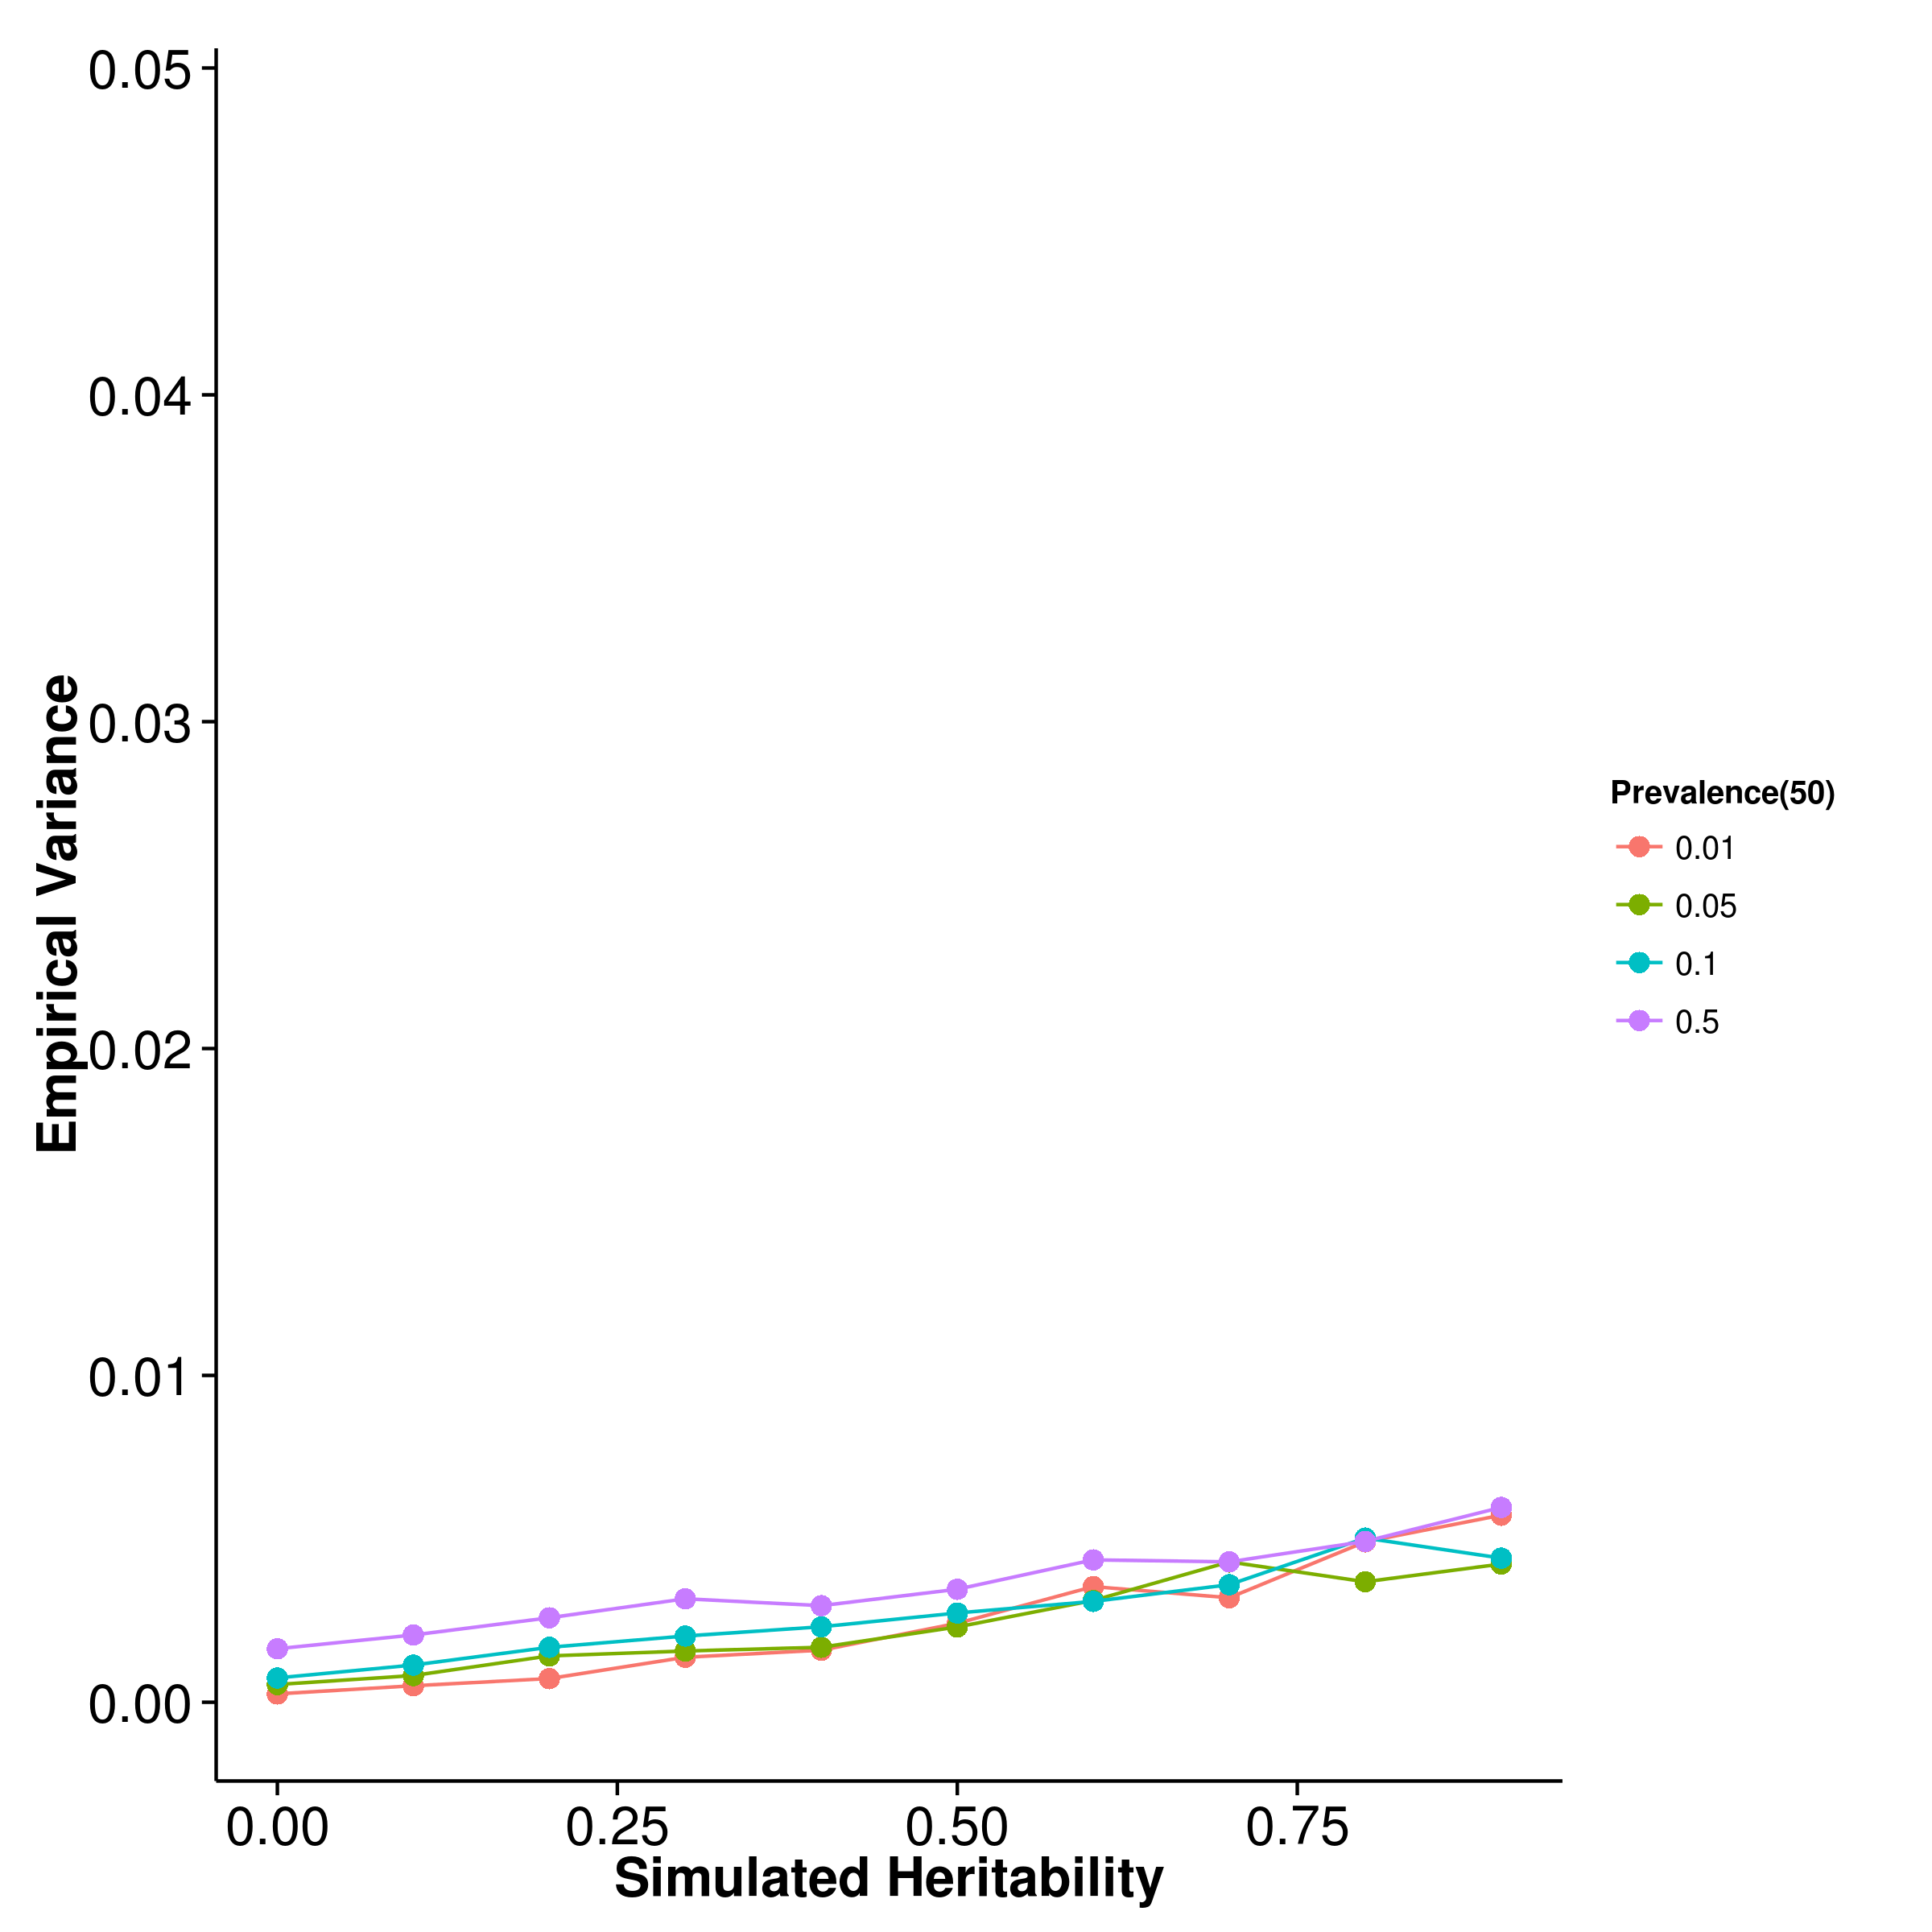
\includegraphics{figure/he_summary/cc_50c/shrek_CC_Rand_sd.png}}
				\label{fig:shrekCC50RandVar}
			}
			\subfloat[GCTA]{
				\scalebox{.4}{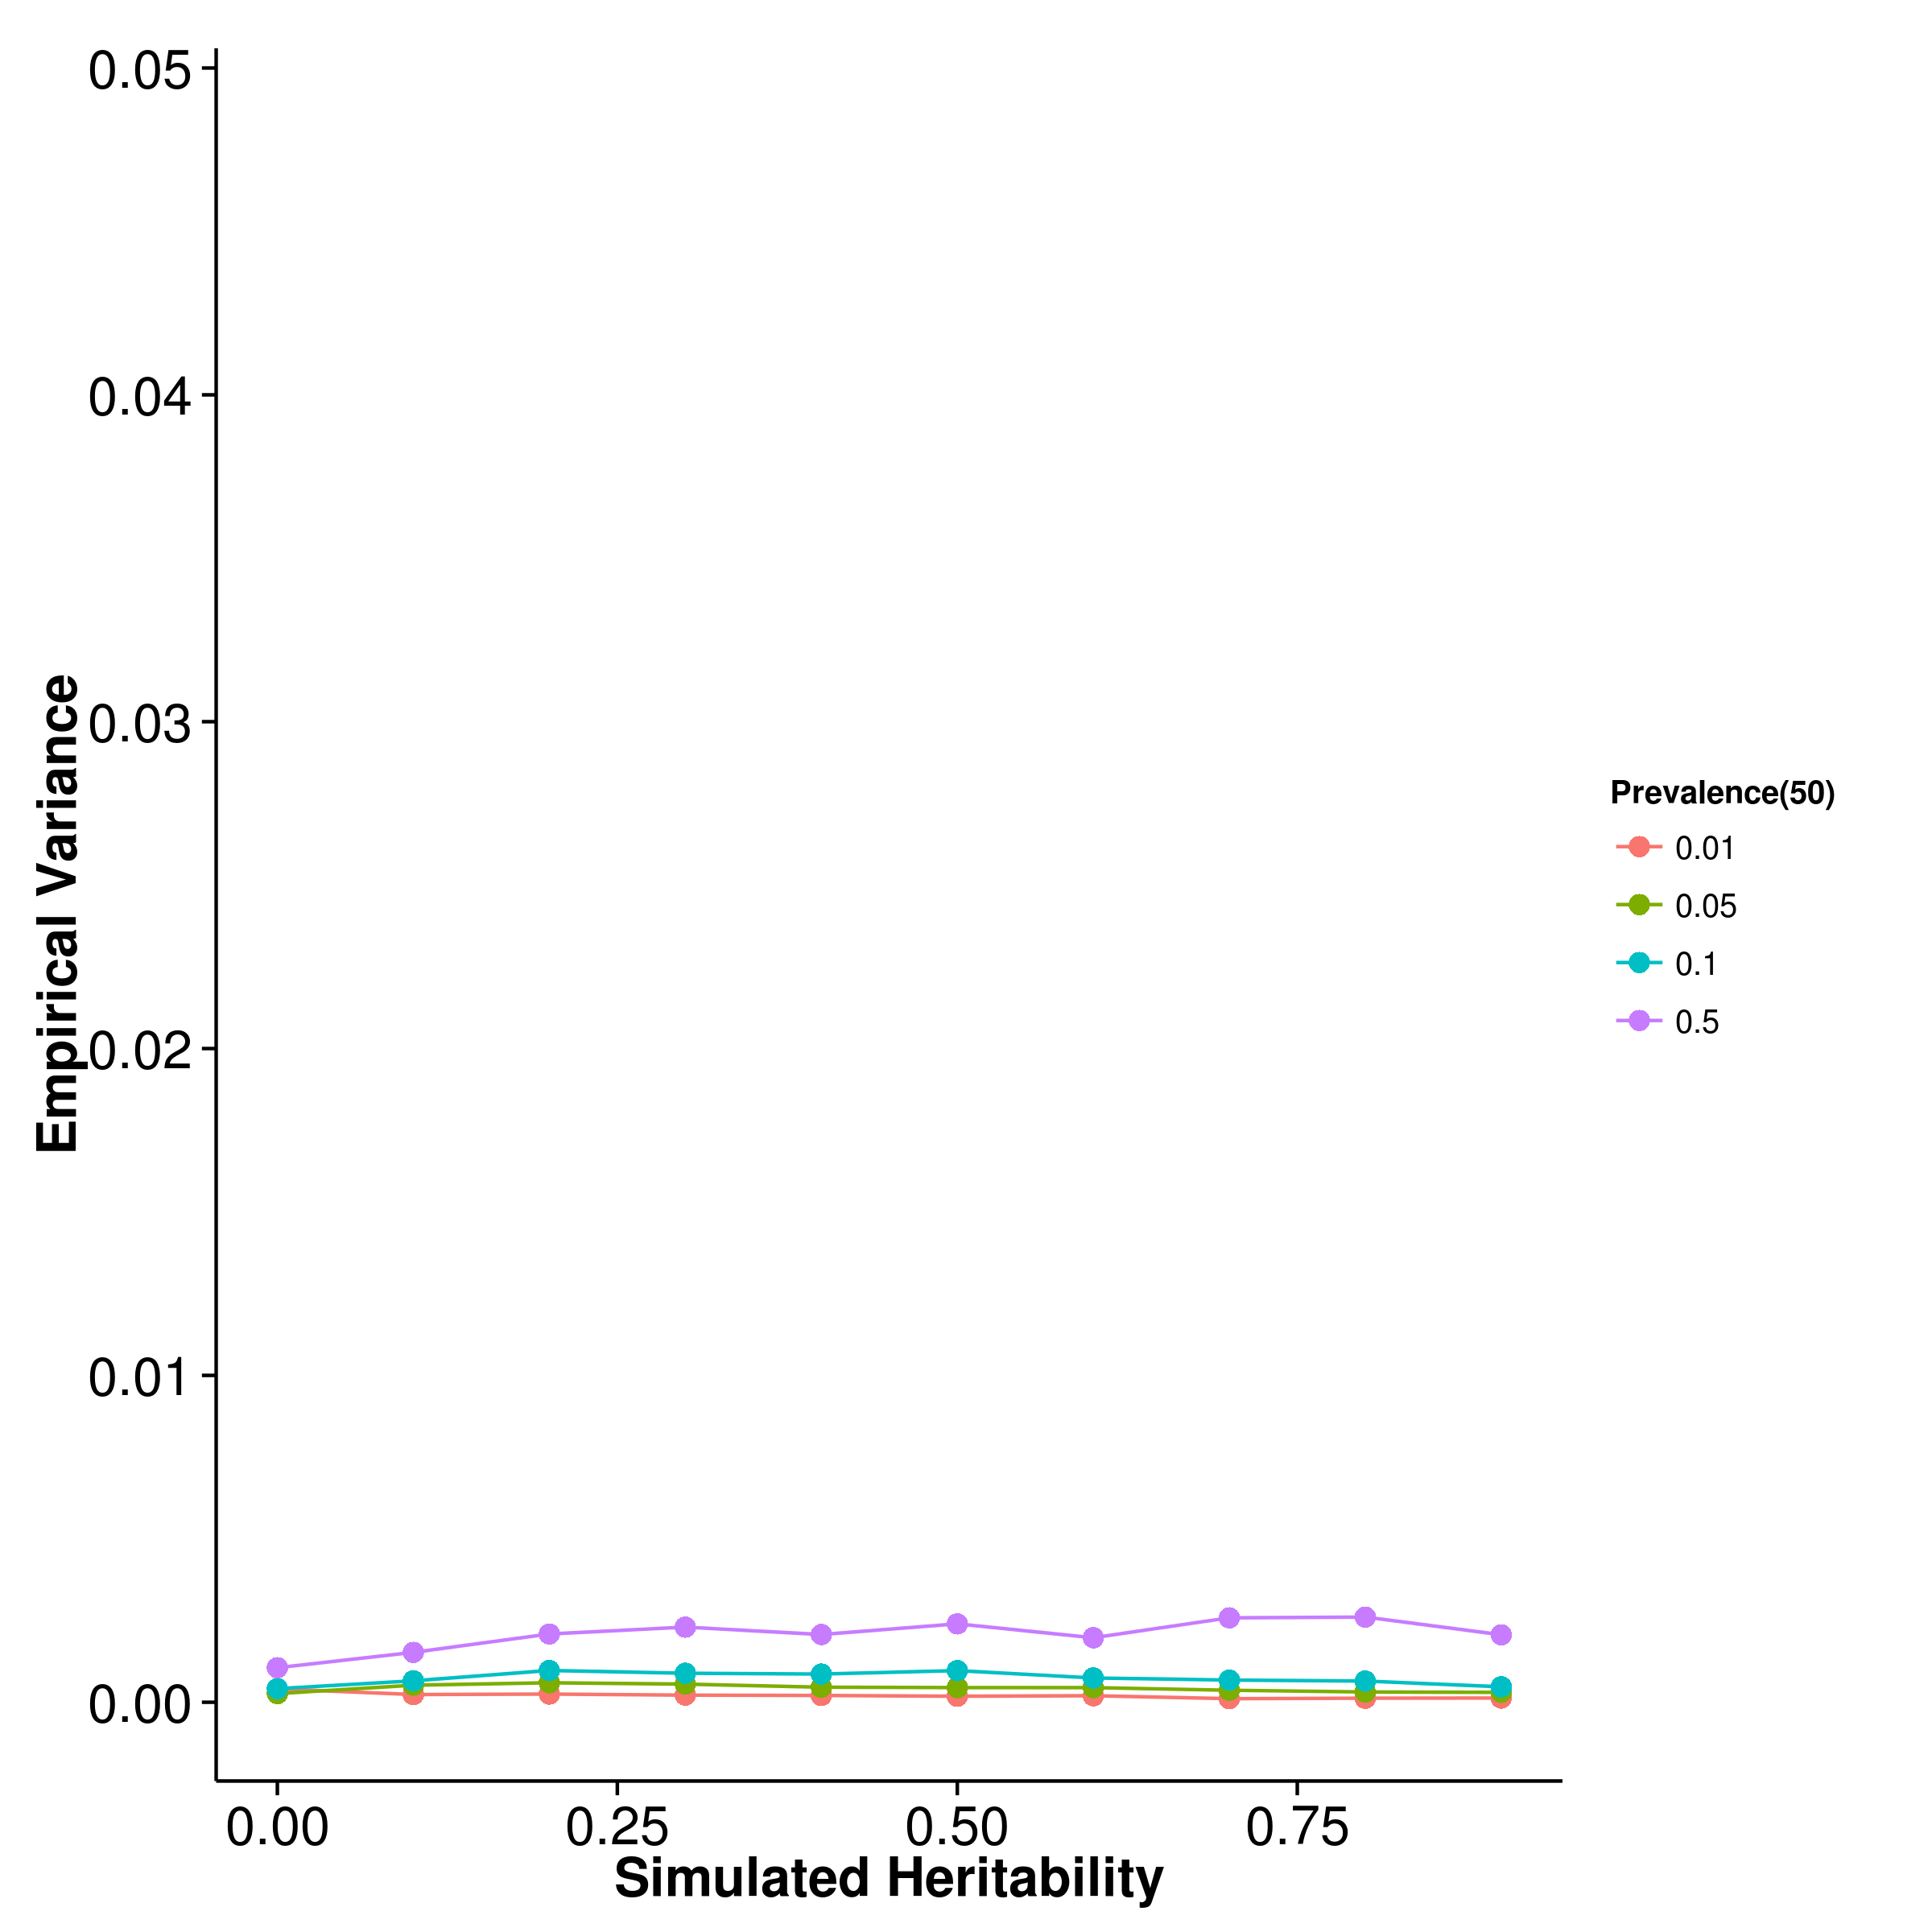
\includegraphics{figure/he_summary/cc_50c/gcta_CC_Rand_sd.png}}
				\label{fig:gctaCC50RandVar}
			}\\
			\subfloat[LDSC with fix intercept]{
				\scalebox{.4}{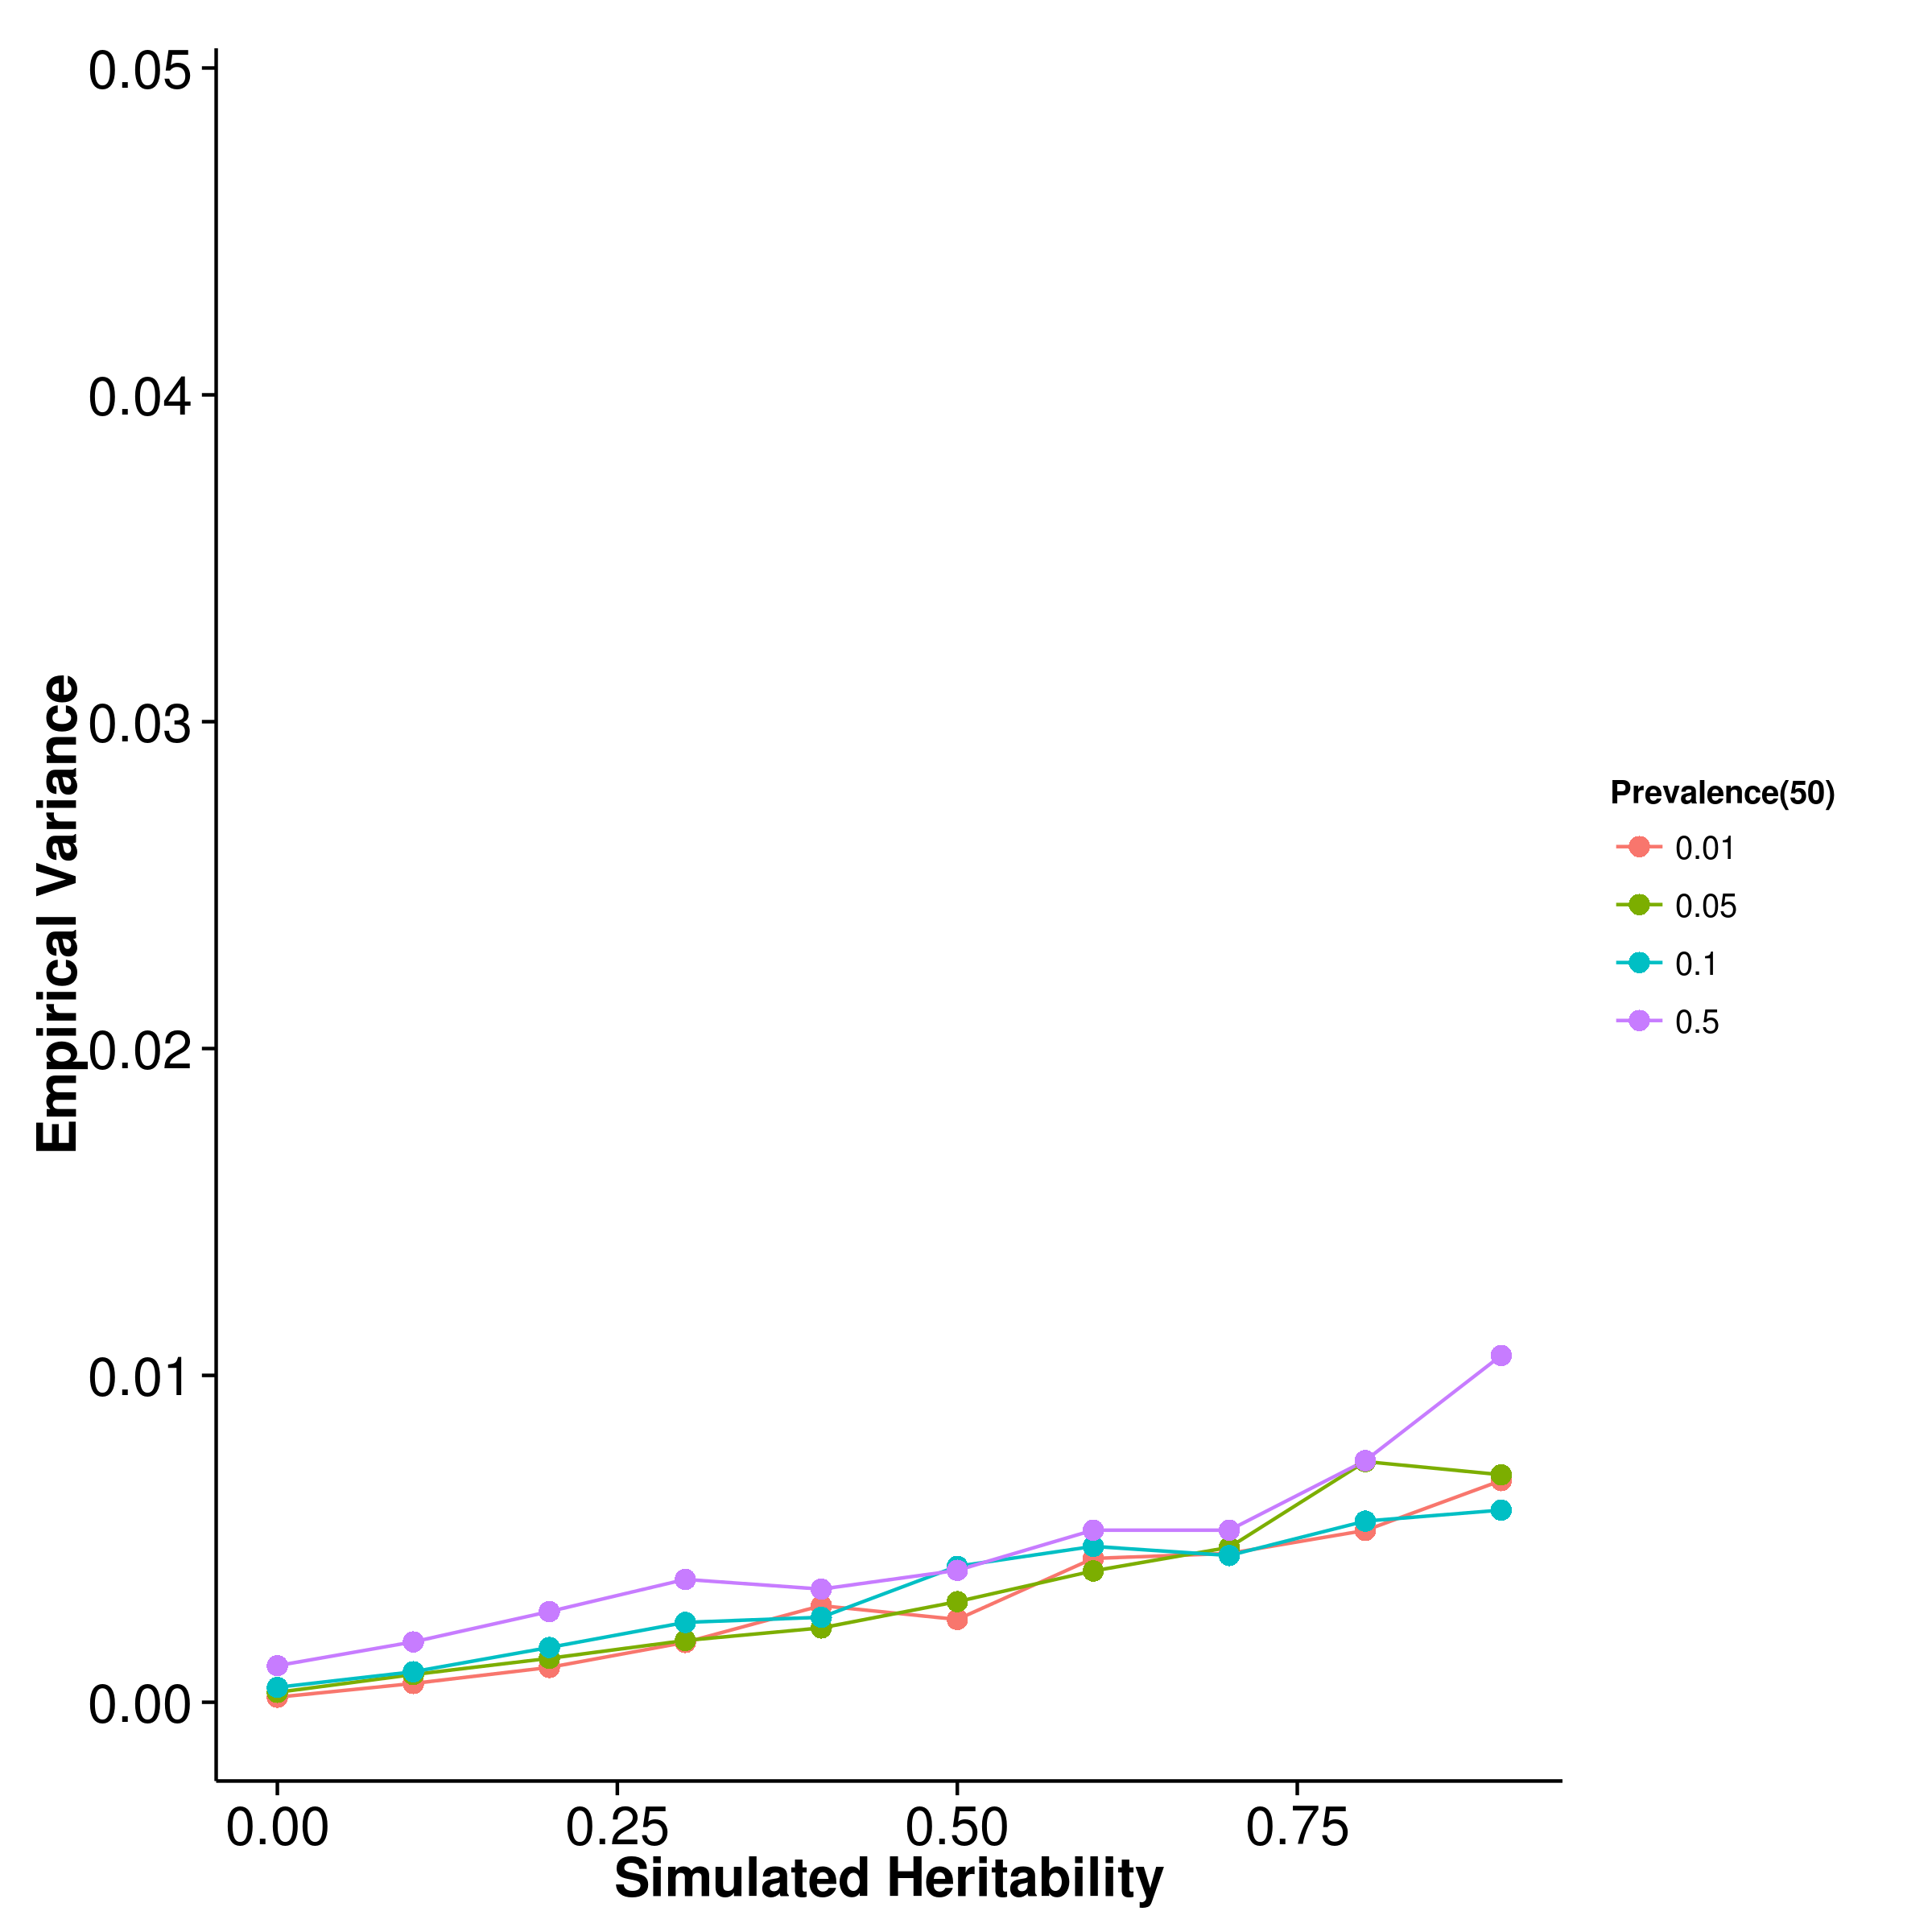
\includegraphics{figure/he_summary/cc_50c/ldsc_CC_Rand_sd.png}}
				\label{fig:ldscCC50RandVar}
			}
			\subfloat[LDSC with intercept estimation]{
				
				\scalebox{.4}{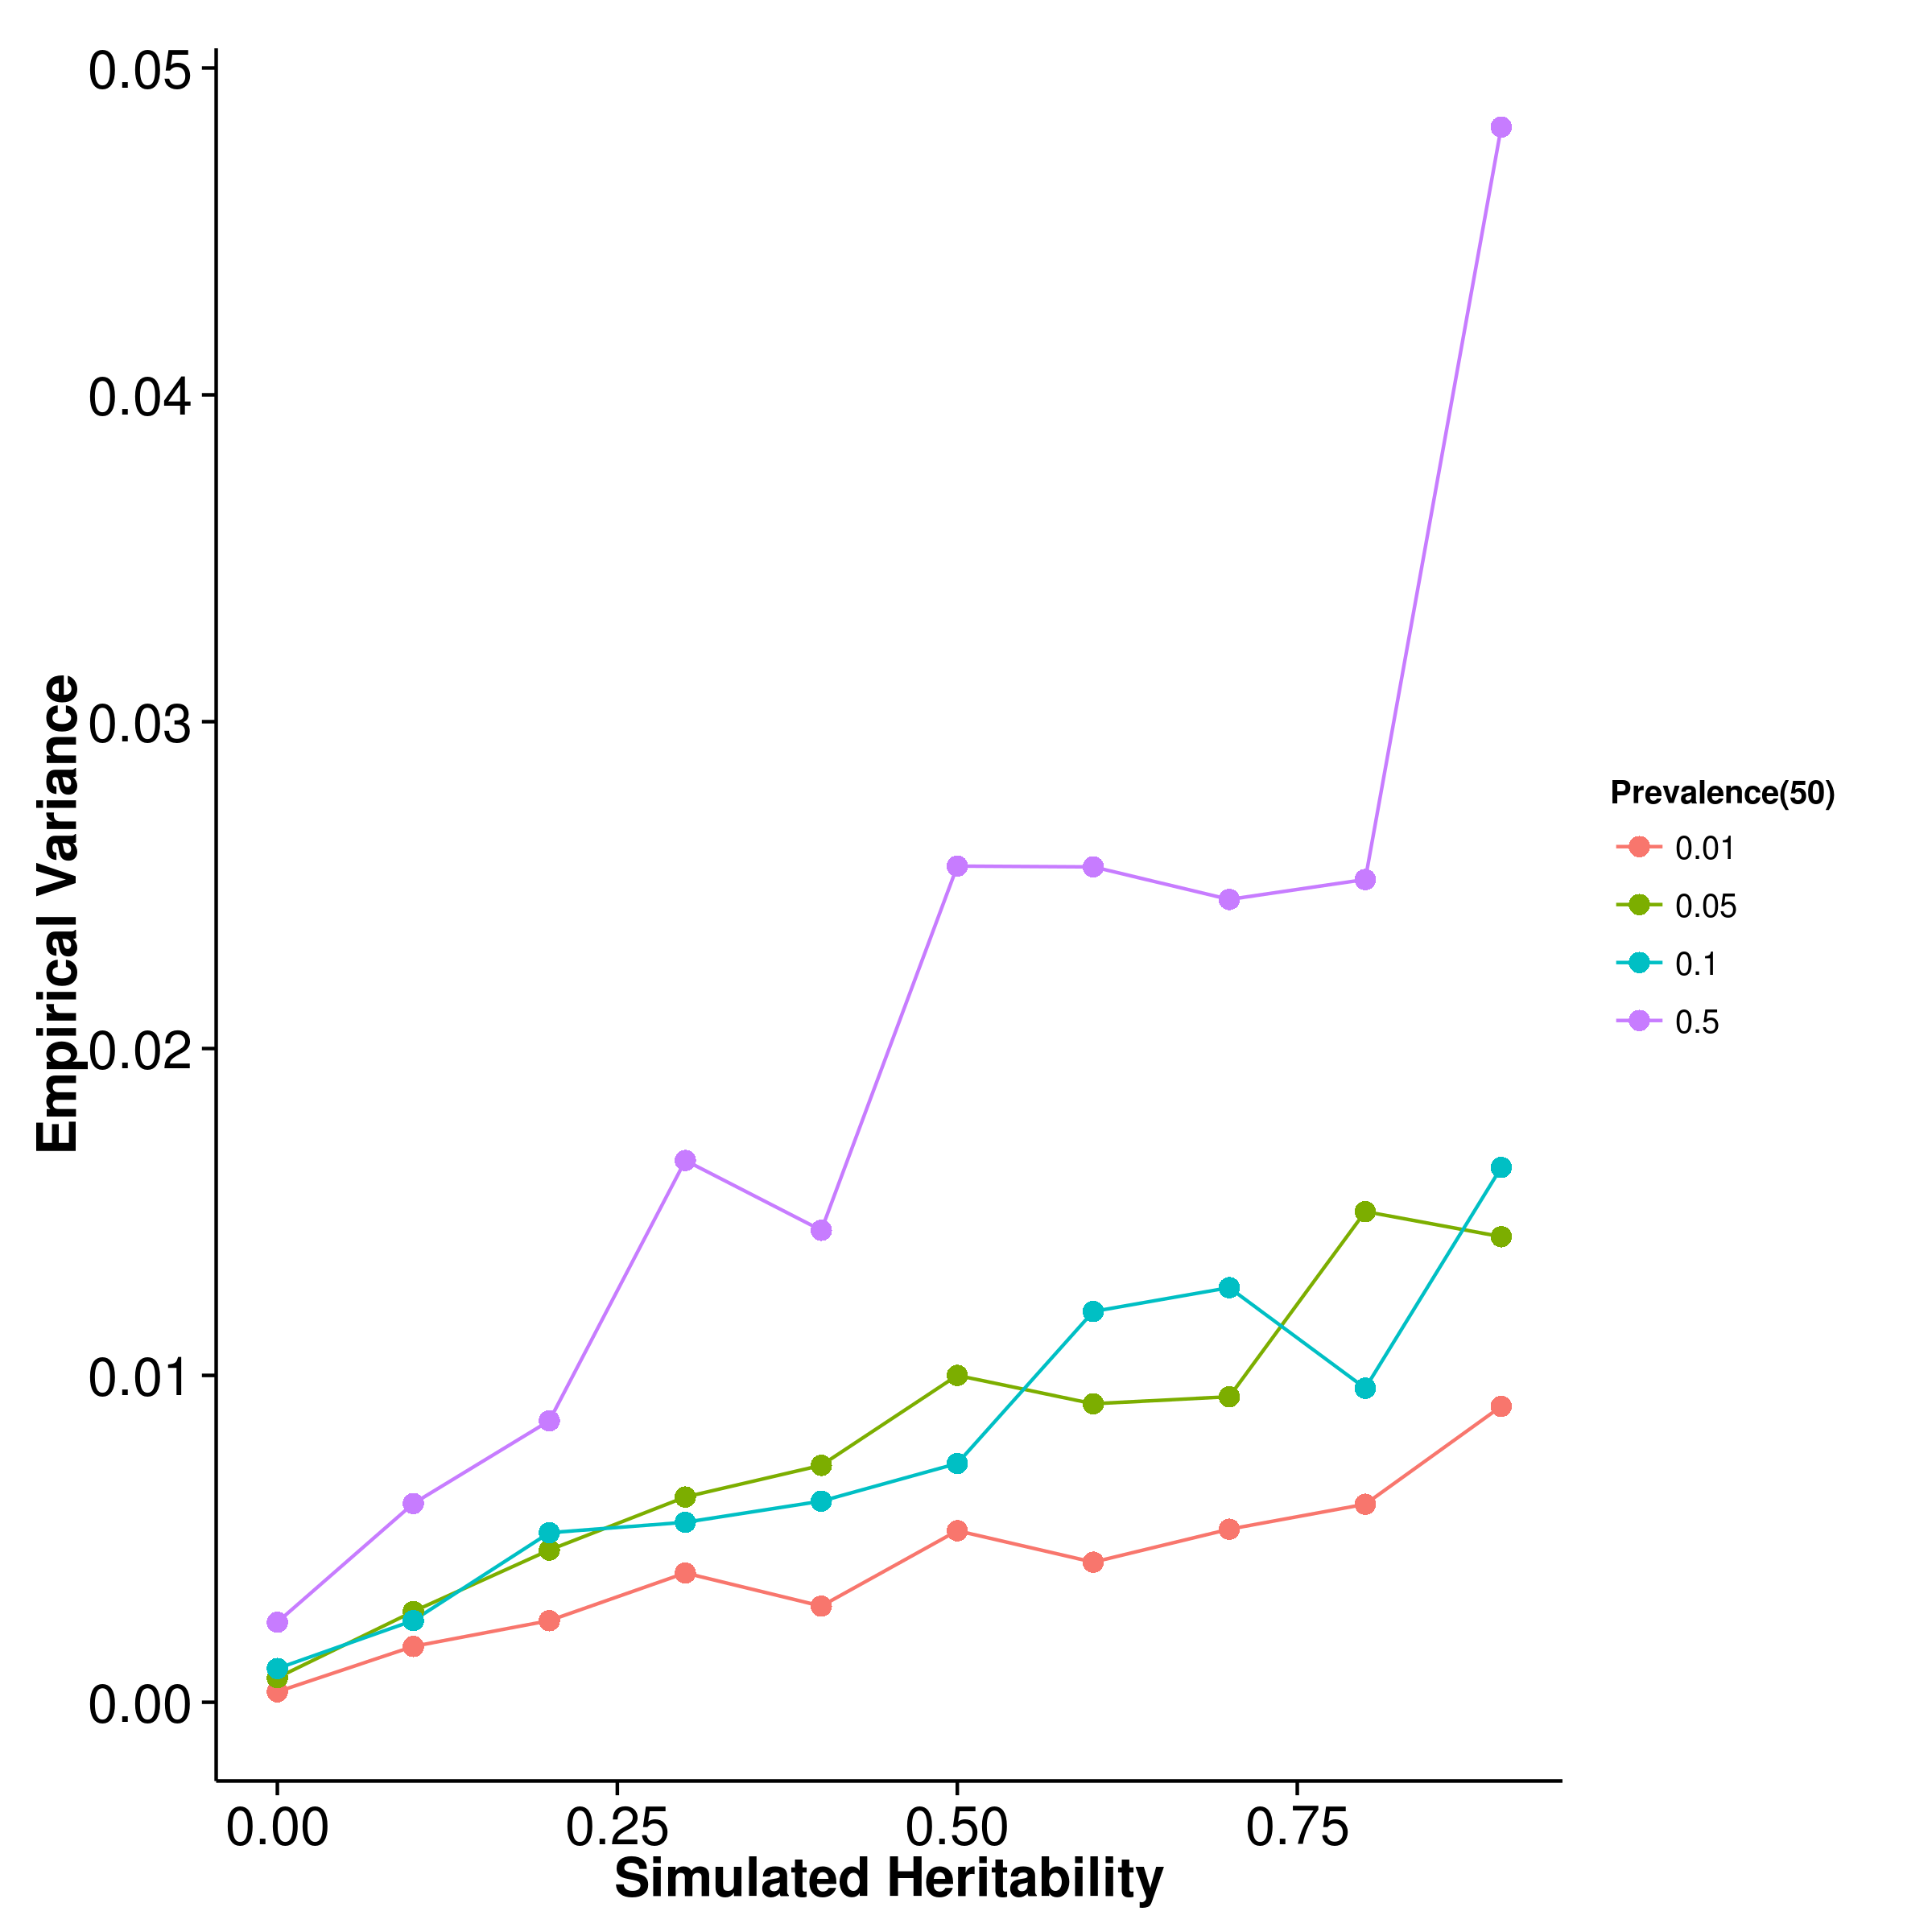
\includegraphics{figure/he_summary/cc_50c/ldscIn_CC_Rand_sd.png}}
				\label{fig:ldscInCC50RandVar}
			}
			\caption[Variance of Case Control Simulation Results (50 Causal)]
			{Variance of results from case control simulation with random effect size simulation with 50 causal \glspl{SNP}.
				For most algorithm except that of \gls{ldsc} with fixed intercept, the empirical variance of the estimates increases as the population prevalence of the trait increases, with the estimations from \gls{ldsc} with intercept estimation display the largest variance.
			} 
			\label{fig:CC50RandVar}
		\end{figure}
		
		
		\begin{figure}
			\centering
			\subfloat[SHREK]{
				\scalebox{.4}{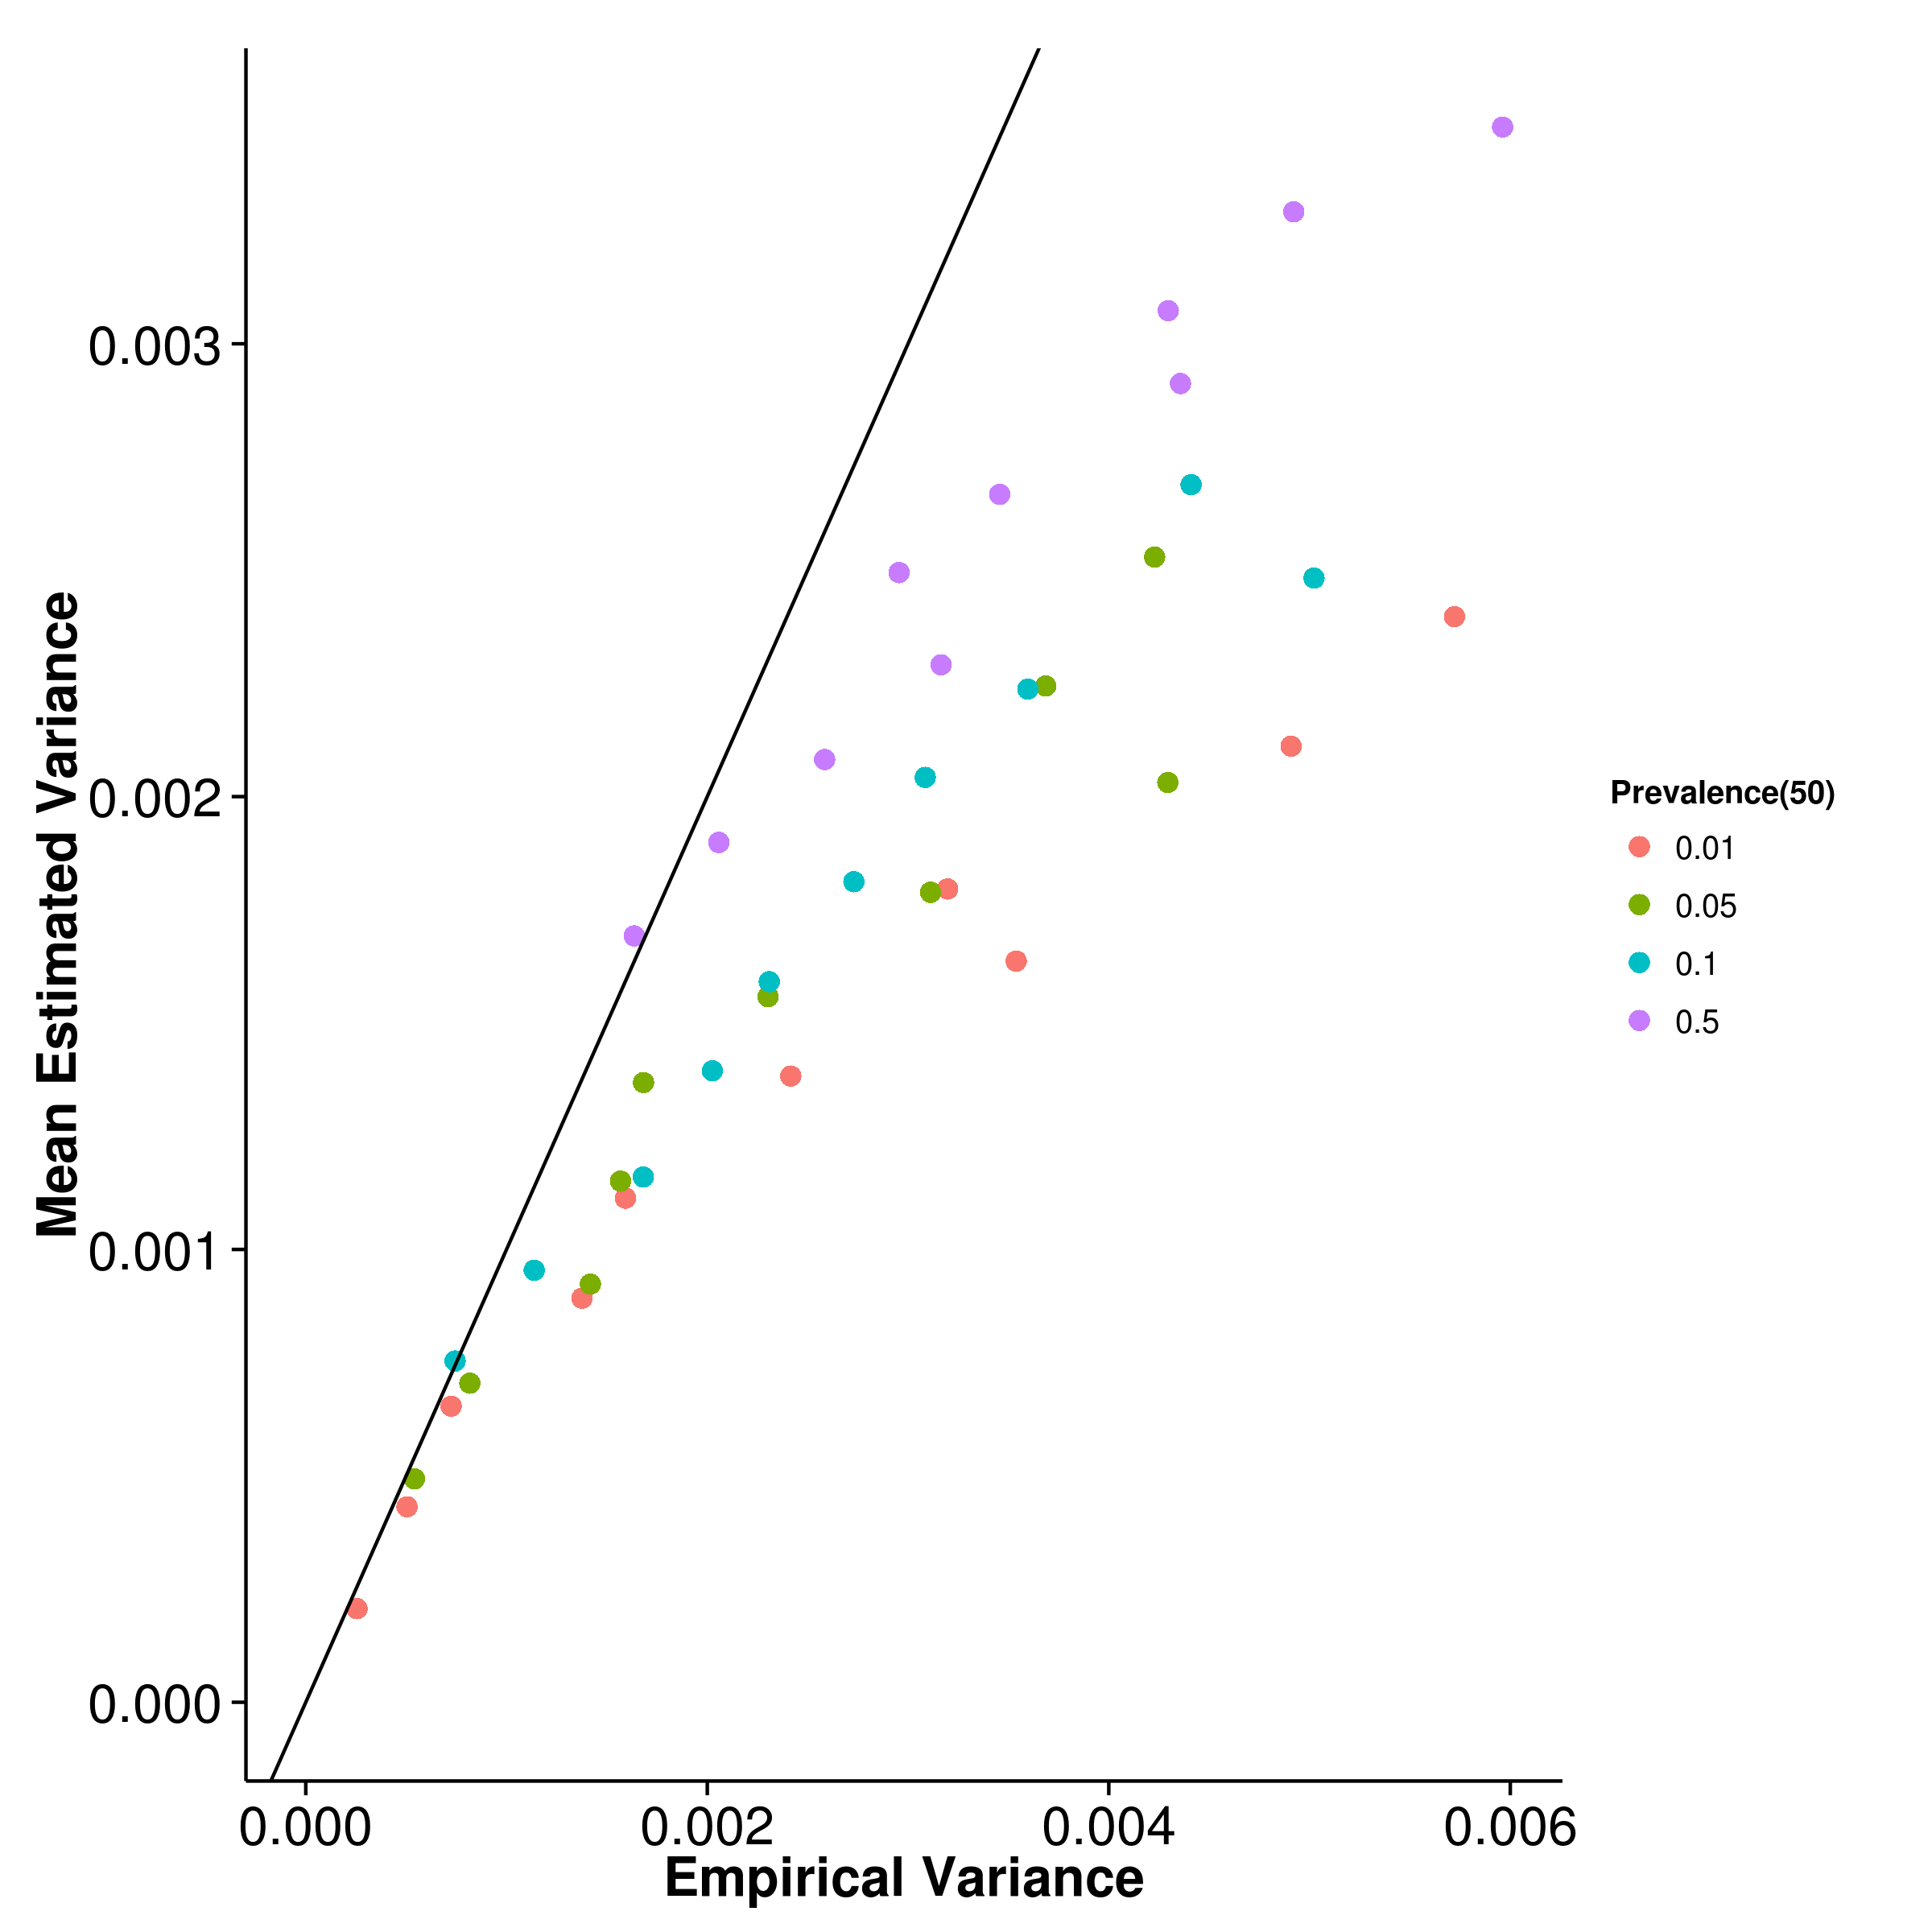
\includegraphics{figure/he_summary/cc_50c/shrek_CC_Rand_sdCom.png}}
				\label{fig:shrekCC50RandVarCom}
			}
			\subfloat[GCTA]{
				\scalebox{.4}{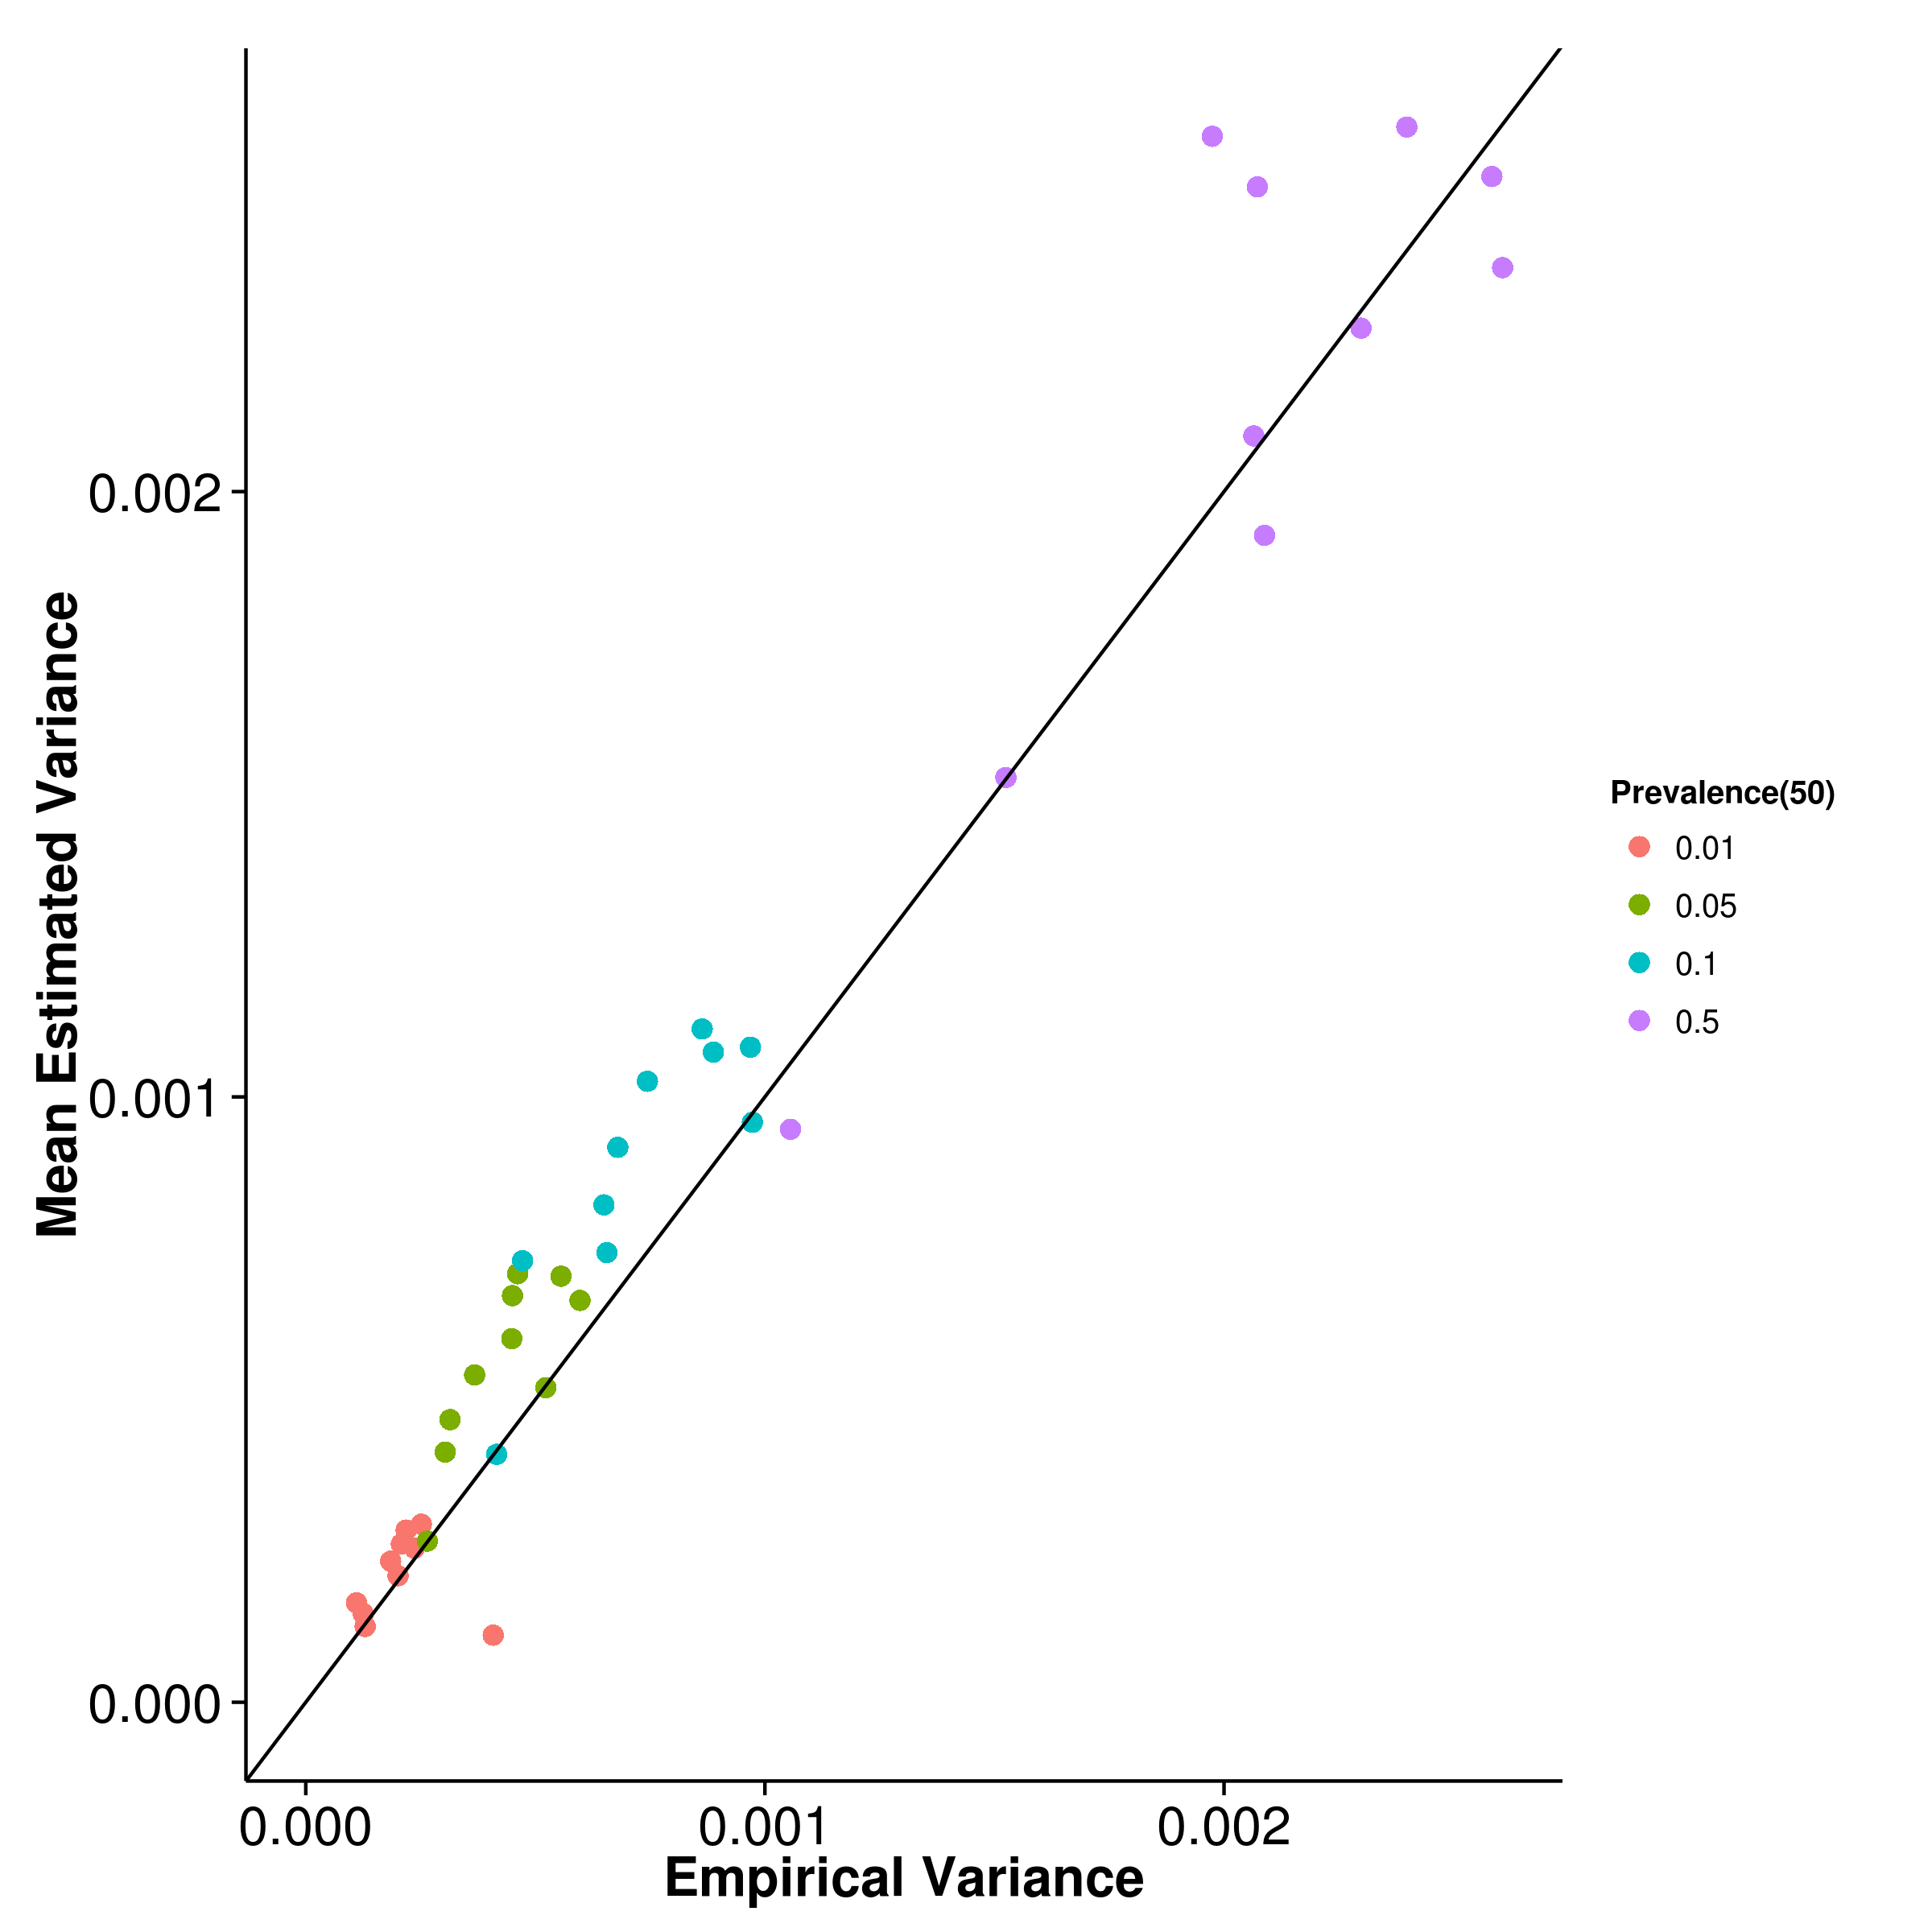
\includegraphics{figure/he_summary/cc_50c/gcta_CC_Rand_sdCom.png}}
				\label{fig:gctaCC50RandVarCom}
			}\\
			\subfloat[LDSC with fix intercept]{
				\scalebox{.4}{\includegraphics{figure/he_summary/cc_50c/ldsc_CC_Rand_sdCom.png}}
				\label{fig:ldscCC50RandVarCom}
			}
			\subfloat[LDSC with intercept estimation]{
				
				\scalebox{.4}{\includegraphics{figure/he_summary/cc_50c/ldscIn_CC_Rand_sdCom.png}}
				\label{fig:ldscInCC50RandVarCom}
			}
			\caption[Estimation of Variance in Case Control Simulation (50 Causal)]
			{Estimated variance of results from case control simulation with random effect size simulation when compared to empirical variance when 50 causal \glspl{SNP} was simulated.
				Again, the estimation of variance from \gls{shrek} tends to be downwardly biased and \gls{ldsc} with fixed intercept tends to be upwardly biased. 
				However, when intercept estimation was performed, the estimation of variance of \gls{ldsc} improved.
			} 
			\label{fig:CC50RandVarCom}
		\end{figure}
		\begin{figure}
			\centering
			\subfloat[SHREK]{
				\scalebox{.4}{\includegraphics{figure/he_summary/cc_100c/shrek_CC_Random_mean.png}}
				\label{fig:shrekCCRandMean}
			}
			\subfloat[GCTA]{
				\scalebox{.4}{\includegraphics{figure/he_summary/cc_100c/gcta_CC_Random_mean.png}}
				\label{fig:gctaCCRandMean}
			}\\
			\subfloat[LDSC with fix intercept]{
				\scalebox{.4}{\includegraphics{figure/he_summary/cc_100c/ldsc_CC_Random_mean.png}}
				\label{fig:ldscCCRandMean}
			}
			\subfloat[LDSC with intercept estimation]{
				
				\scalebox{.4}{\includegraphics{figure/he_summary/cc_100c/ldscIn_CC_Random_mean.png}}
				\label{fig:ldscInCCRandMean}
			}
			\caption[Case Control with Random Effect Size Simulation Result(Mean)]
			{Mean of results from case control simulation with random effect size simulation.
				The performance of \gls{gcta} was as suggested by \citet{Golan2014} where there was an underestimation as prevalence decreases.
				On the other hand, \gls{ldsc} were upwardly biased when a fixed intercept was used and this bias was corrected when an estimation of intercept was allowed.
				\gls{shrek} does not seems to as sensitive to change in prevalence and the estimation were relatively robust.
				} 
			\label{fig:CCRandMean}
		\end{figure}
		
		\begin{figure}
			\centering
			\subfloat[SHREK]{
				\scalebox{.4}{\includegraphics{figure/he_summary/cc_100c/shrek_CC_Random_sd.png}}
				\label{fig:shrekCCRandVar}
			}
			\subfloat[GCTA]{
				\scalebox{.4}{\includegraphics{figure/he_summary/cc_100c/gcta_CC_Random_sd.png}}
				\label{fig:gctaCCRandVar}
			}\\
			\subfloat[LDSC with fix intercept]{
				\scalebox{.4}{\includegraphics{figure/he_summary/cc_100c/ldsc_CC_Random_sd.png}}
				\label{fig:ldscCCRandVar}
			}
			\subfloat[LDSC with intercept estimation]{
				
				\scalebox{.4}{\includegraphics{figure/he_summary/cc_100c/ldscIn_CC_Random_sd.png}}
				\label{fig:ldscInCCRandVar}
			}
			\caption[Case Control with Random Effect Size Simulation Result(Variance)]
			{Variance of results from case control simulation with random effect size simulation.
				It was clear that the prevalence affects the variance of estimation where a larger variance tends to increase the variance of estimation.
				Again, \gls{gcta} has the lowest variance, however, unlike in the quantitative trait simulation, \gls{shrek} has a lower average variance when compared to \gls{ldsc} with fixed intercept.
				Nonetheless, it was important to remember that in case control simulation, a much smaller amount of \glspl{SNP} was used, thus the results was not directly comparable to results from the quantitative simulation.
			} 
			\label{fig:CCRandVar}
		\end{figure}
		
		
		\begin{figure}
			\centering
			\subfloat[SHREK]{
				\scalebox{.4}{\includegraphics{figure/he_summary/cc_100c/shrek_CC_Random_sdCom.png}}
				\label{fig:shrekCCRandVarCom}
			}
			\subfloat[GCTA]{
				\scalebox{.4}{\includegraphics{figure/he_summary/cc_100c/gcta_CC_Random_sdCom.png}}
				\label{fig:gctaCCRandVarCom}
			}\\
			\subfloat[LDSC with fix intercept]{
				\scalebox{.4}{\includegraphics{figure/he_summary/cc_100c/ldsc_CC_Random_sdCom.png}}
				\label{fig:ldscCCRandVarCom}
			}
			\subfloat[LDSC with intercept estimation]{
				
				\scalebox{.4}{\includegraphics{figure/he_summary/cc_100c/ldscIn_CC_Random_sdCom.png}}
				\label{fig:ldscInCCRandVarCom}
			}
			\caption[Case Control with Random Effect Size Simulation Result(Estimated Variance)]
			{Estimated variance of results from case control simulation with random effect size simulation when compared to empirical variance.
				From the quantitative trait simulation with random effect size(\cref{fig:QtRandVarCom}), it was observed that the variance estimation of \gls{shrek} and \gls{gcta} were rater accurate.
				Similarly, in the case control simulation with 100 causal \glspl{SNP}, it was observed that the variance estimation of \gls{shrek} and \gls{gcta} were close to the empirical variance with slight bias.
				A large up-ward bias was observed for \gls{ldsc} with fixed intercept estimation but the bias was less when \gls{ldsc} was allowed to estimate the intercept.s
			} 
			\label{fig:CCRandVarCom}
		\end{figure}
			\begin{figure}
			\centering
			\subfloat[SHREK]{
				\scalebox{.4}{\includegraphics{figure/he_summary/cc_500c/shrek_CC_Rand_mean.png}}
				\label{fig:shrekCC500RandMean}
			}
			\subfloat[GCTA]{
				\scalebox{.4}{\includegraphics{figure/he_summary/cc_500c/gcta_CC_Rand_mean.png}}
				\label{fig:gctaCC500RandMean}
			}\\
			\subfloat[LDSC with fix intercept]{
				\scalebox{.4}{\includegraphics{figure/he_summary/cc_500c/ldsc_CC_Rand_mean.png}}
				\label{fig:ldscCC500RandMean}
			}
			\subfloat[LDSC with intercept estimation]{
				
				\scalebox{.4}{\includegraphics{figure/he_summary/cc_500c/ldscIn_CC_Rand_mean.png}}
				\label{fig:ldscInCC500RandMean}
			}
			\caption[Mean of Case Control Simulation Results (500 Causal)]
			{Mean of results from case control simulation with random effect size simulation with 500 causal \glspl{SNP}.
				Again, a clear pattern of underestimation was observed for \gls{gcta} and \gls{ldsc} with intercept estimation whereas estimations from \gls{shrek} and \gls{ldsc} with fixed intercepts tends to be upwardly biased, with the magnitude of bias increases as the population prevalence decreases.
				} 
			\label{fig:CC500RandMean}
		\end{figure}
		
		\begin{figure}
			\centering
			\subfloat[SHREK]{
				\scalebox{.4}{\includegraphics{figure/he_summary/cc_500c/shrek_CC_Rand_sd.png}}
				\label{fig:shrekCC500RandVar}
			}
			\subfloat[GCTA]{
				\scalebox{.4}{\includegraphics{figure/he_summary/cc_500c/gcta_CC_Rand_sd.png}}
				\label{fig:gctaCC500RandVar}
			}\\
			\subfloat[LDSC with fix intercept]{
				\scalebox{.4}{\includegraphics{figure/he_summary/cc_500c/ldsc_CC_Rand_sd.png}}
				\label{fig:ldscCC500RandVar}
			}
			\subfloat[LDSC with intercept estimation]{
				
				\scalebox{.4}{\includegraphics{figure/he_summary/cc_500c/ldscIn_CC_Rand_sd.png}}
				\label{fig:ldscInCC500RandVar}
			}
			\caption[Variance of Case Control Simulation Results (500 Causal)]
			{Variance of results from case control simulation with random effect size simulation with 500 causal \glspl{SNP}.
				As the number of causal \glspl{SNP} increased to 500, the empirical variance of \gls{shrek} and \gls{ldsc} with fixed intercept converges. 
				However, the empirical variance of \gls{ldsc} with intercept estimations remains high. 
			} 
			\label{fig:CC500RandVar}
		\end{figure}
		
		
		\begin{figure}
			\centering
			\subfloat[SHREK]{
				\scalebox{.4}{\includegraphics{figure/he_summary/cc_500c/shrek_CC_Rand_sdCom.png}}
				\label{fig:shrekCC500RandVarCom}
			}
			\subfloat[GCTA]{
				\scalebox{.4}{\includegraphics{figure/he_summary/cc_500c/gcta_CC_Rand_sdCom.png}}
				\label{fig:gctaCC500RandVarCom}
			}\\
			\subfloat[LDSC with fix intercept]{
				\scalebox{.4}{\includegraphics{figure/he_summary/cc_500c/ldsc_CC_Rand_sdCom.png}}
				\label{fig:ldscCC500RandVarCom}
			}
			\subfloat[LDSC with intercept estimation]{
				
				\scalebox{.4}{\includegraphics{figure/he_summary/cc_500c/ldscIn_CC_Rand_sdCom.png}}
				\label{fig:ldscInCC500RandVarCom}
			}
			\caption[Estimation of Variance in Case Control Simulation (500 Causal)]
			{Estimated variance of results from case control simulation with random effect size simulation when compared to empirical variance when 500 causal \glspl{SNP} was simulated.
				When the trait contains 500 causal \glspl{SNP}, \gls{ldsc} begins to provide a good estimation of its own empirical variance both with and without intercept estimation. 
				On the other hand, \gls{shrek}'s estimation of its own empirical variance remains consistently lower than the true empirical variance.
			} 
			\label{fig:CC500RandVarCom}
		\end{figure}
		Finally, for the case control simulation, we simulated 
		
		\subsection{Extreme Phenotype Simulation}
		%TODO compare the result to that of the quantitative simulation, there is no increase in power though...
		
	\section{Discussion}

	
	%Put these graphs in supplementary instead